\graphicspath{{./Figs/}}

\chapter{Results and Discussion} 

\section{Wind Tunnel Results}
This chapter outlines the final wind tunnel results for all three main configurations; tractor, pusher and no propeller. It outlines the main trends in the stability coefficients Cl, Cn, and Cm corresponding to the MAV model's roll, yaw and pitch. These results are analysed with critical observations and trends identified. A validation of the wind tunnel results is also conducted with VAP 3.5 to compare the accuracy of the results obtained with any discrepancies explained.

\todo{Table of variables/geometry which defines the MAV}


\subsection{Aerodynamic Coefficient of Lift}
\Cref{fig:Cl_10ms_6000} and \Cref{fig:Cl_10ms_11000} show that as the motor speed increases from 6000RPM to 11000RPM the coefficient of lift increases slightly for both the tractor and pusher configurations. As typically seen in aircraft\todo{add citation}, the lift curve also does not drop off. The tractor configuration sees an increase in the lift coefficient beyond the stall point, while the pusher configuration has a linear decrease in the lift coefficient beyond the stall point. Increasing the airspeed to 20m$s^{-1}$ at the higher 11000RPM speed delays the MAV model's stall as the angle of attack increases in all configurations. Increasing the airspeed when the motor is at 6000RPM increases the max coefficient of lift seen for the pusher configuration \todo{ADD VALUES} and delays stall. The tractor configuration has a deeper stall beyond the stall point when airspeed is at 20m$s^{-1}$, and leads to a more unrecoverable aircraft if stall were to occur as the MAV would experience extremely high angles of attack. It also gives little room for error or warning in order to correct the MAVs position in order to avoid a stall. These trends due to airspeed are shown between \Cref{fig:Cl_10ms_6000} and \Cref{fig:Cl_20ms_6000} as well as between \Cref{fig:Cl_10ms_11000} and \Cref{fig:Cl_20ms_11000}.

\begin{figure}[H]
    \centering
    \begin{subfigure}[b]{0.467\textwidth}
        \centering
        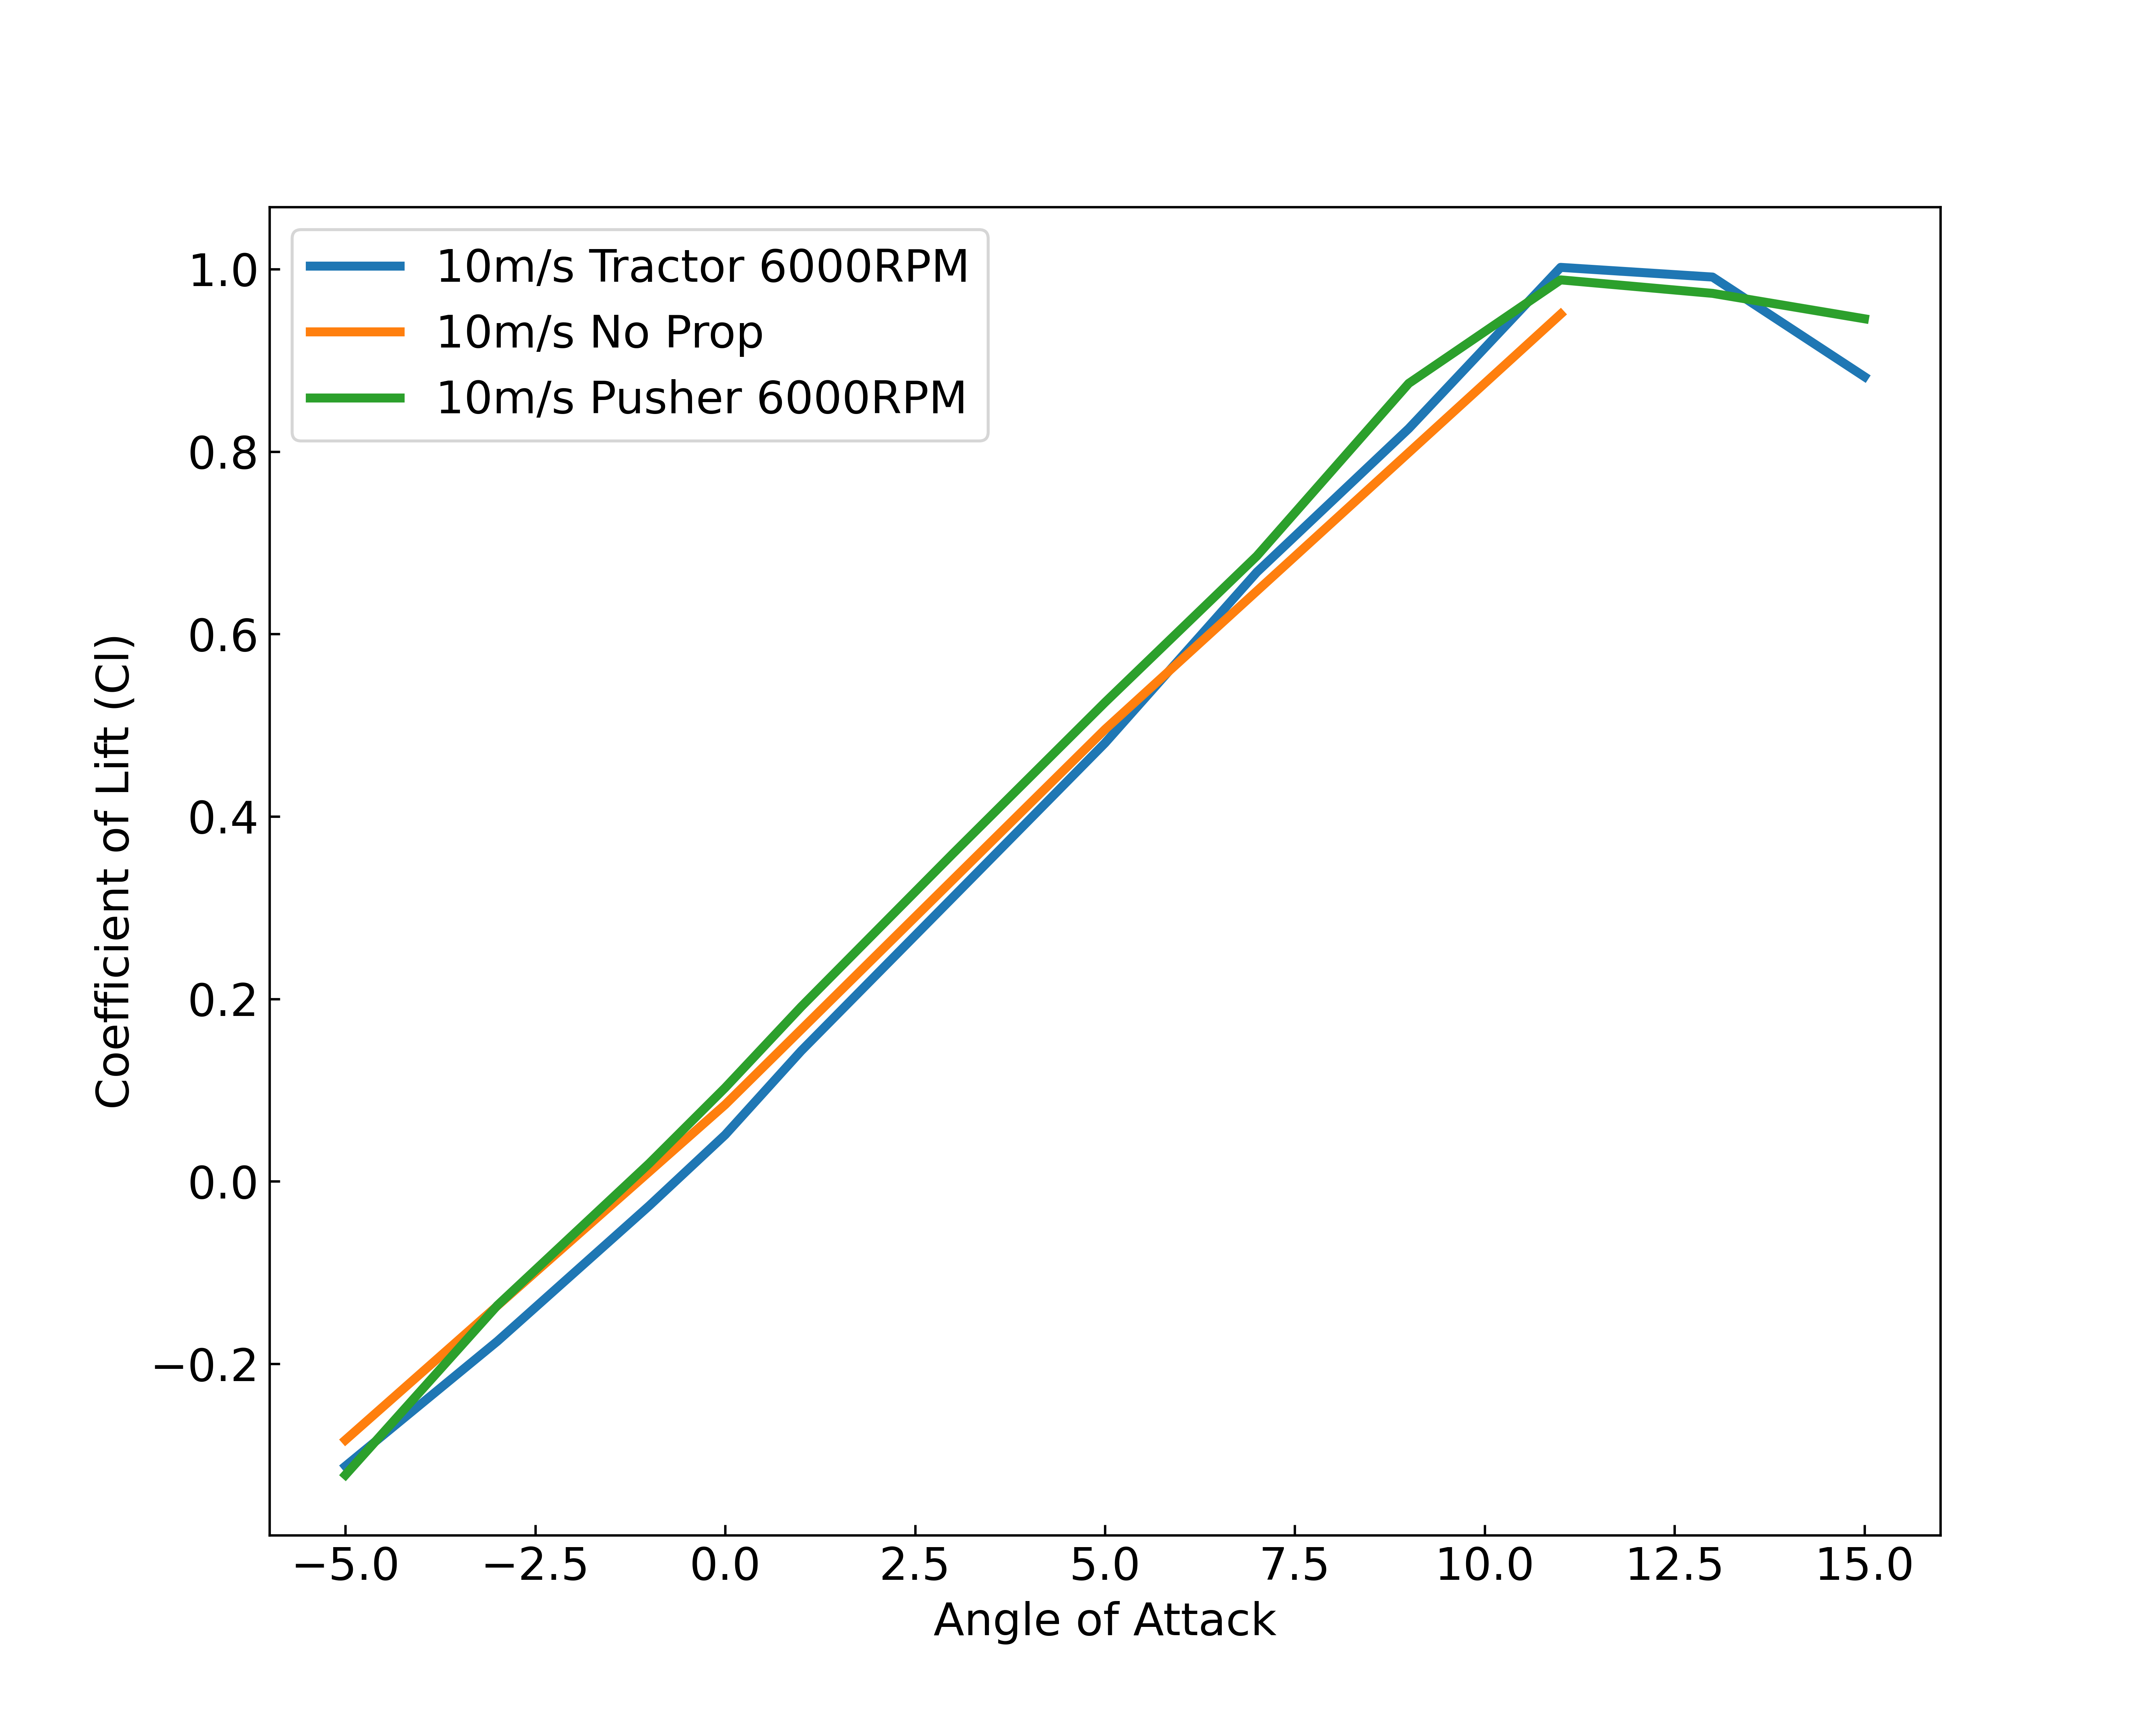
\includegraphics[width=\textwidth]{05_Results/Figs/Cl/10ms_6000RPM_Cl.png}
        \caption{Coefficient of lift at 10m/s airspeed and 6000RPM motor speed}
        \label{fig:Cl_10ms_6000}
    \end{subfigure}
    \begin{subfigure}[b]{0.467\textwidth}
        \centering
        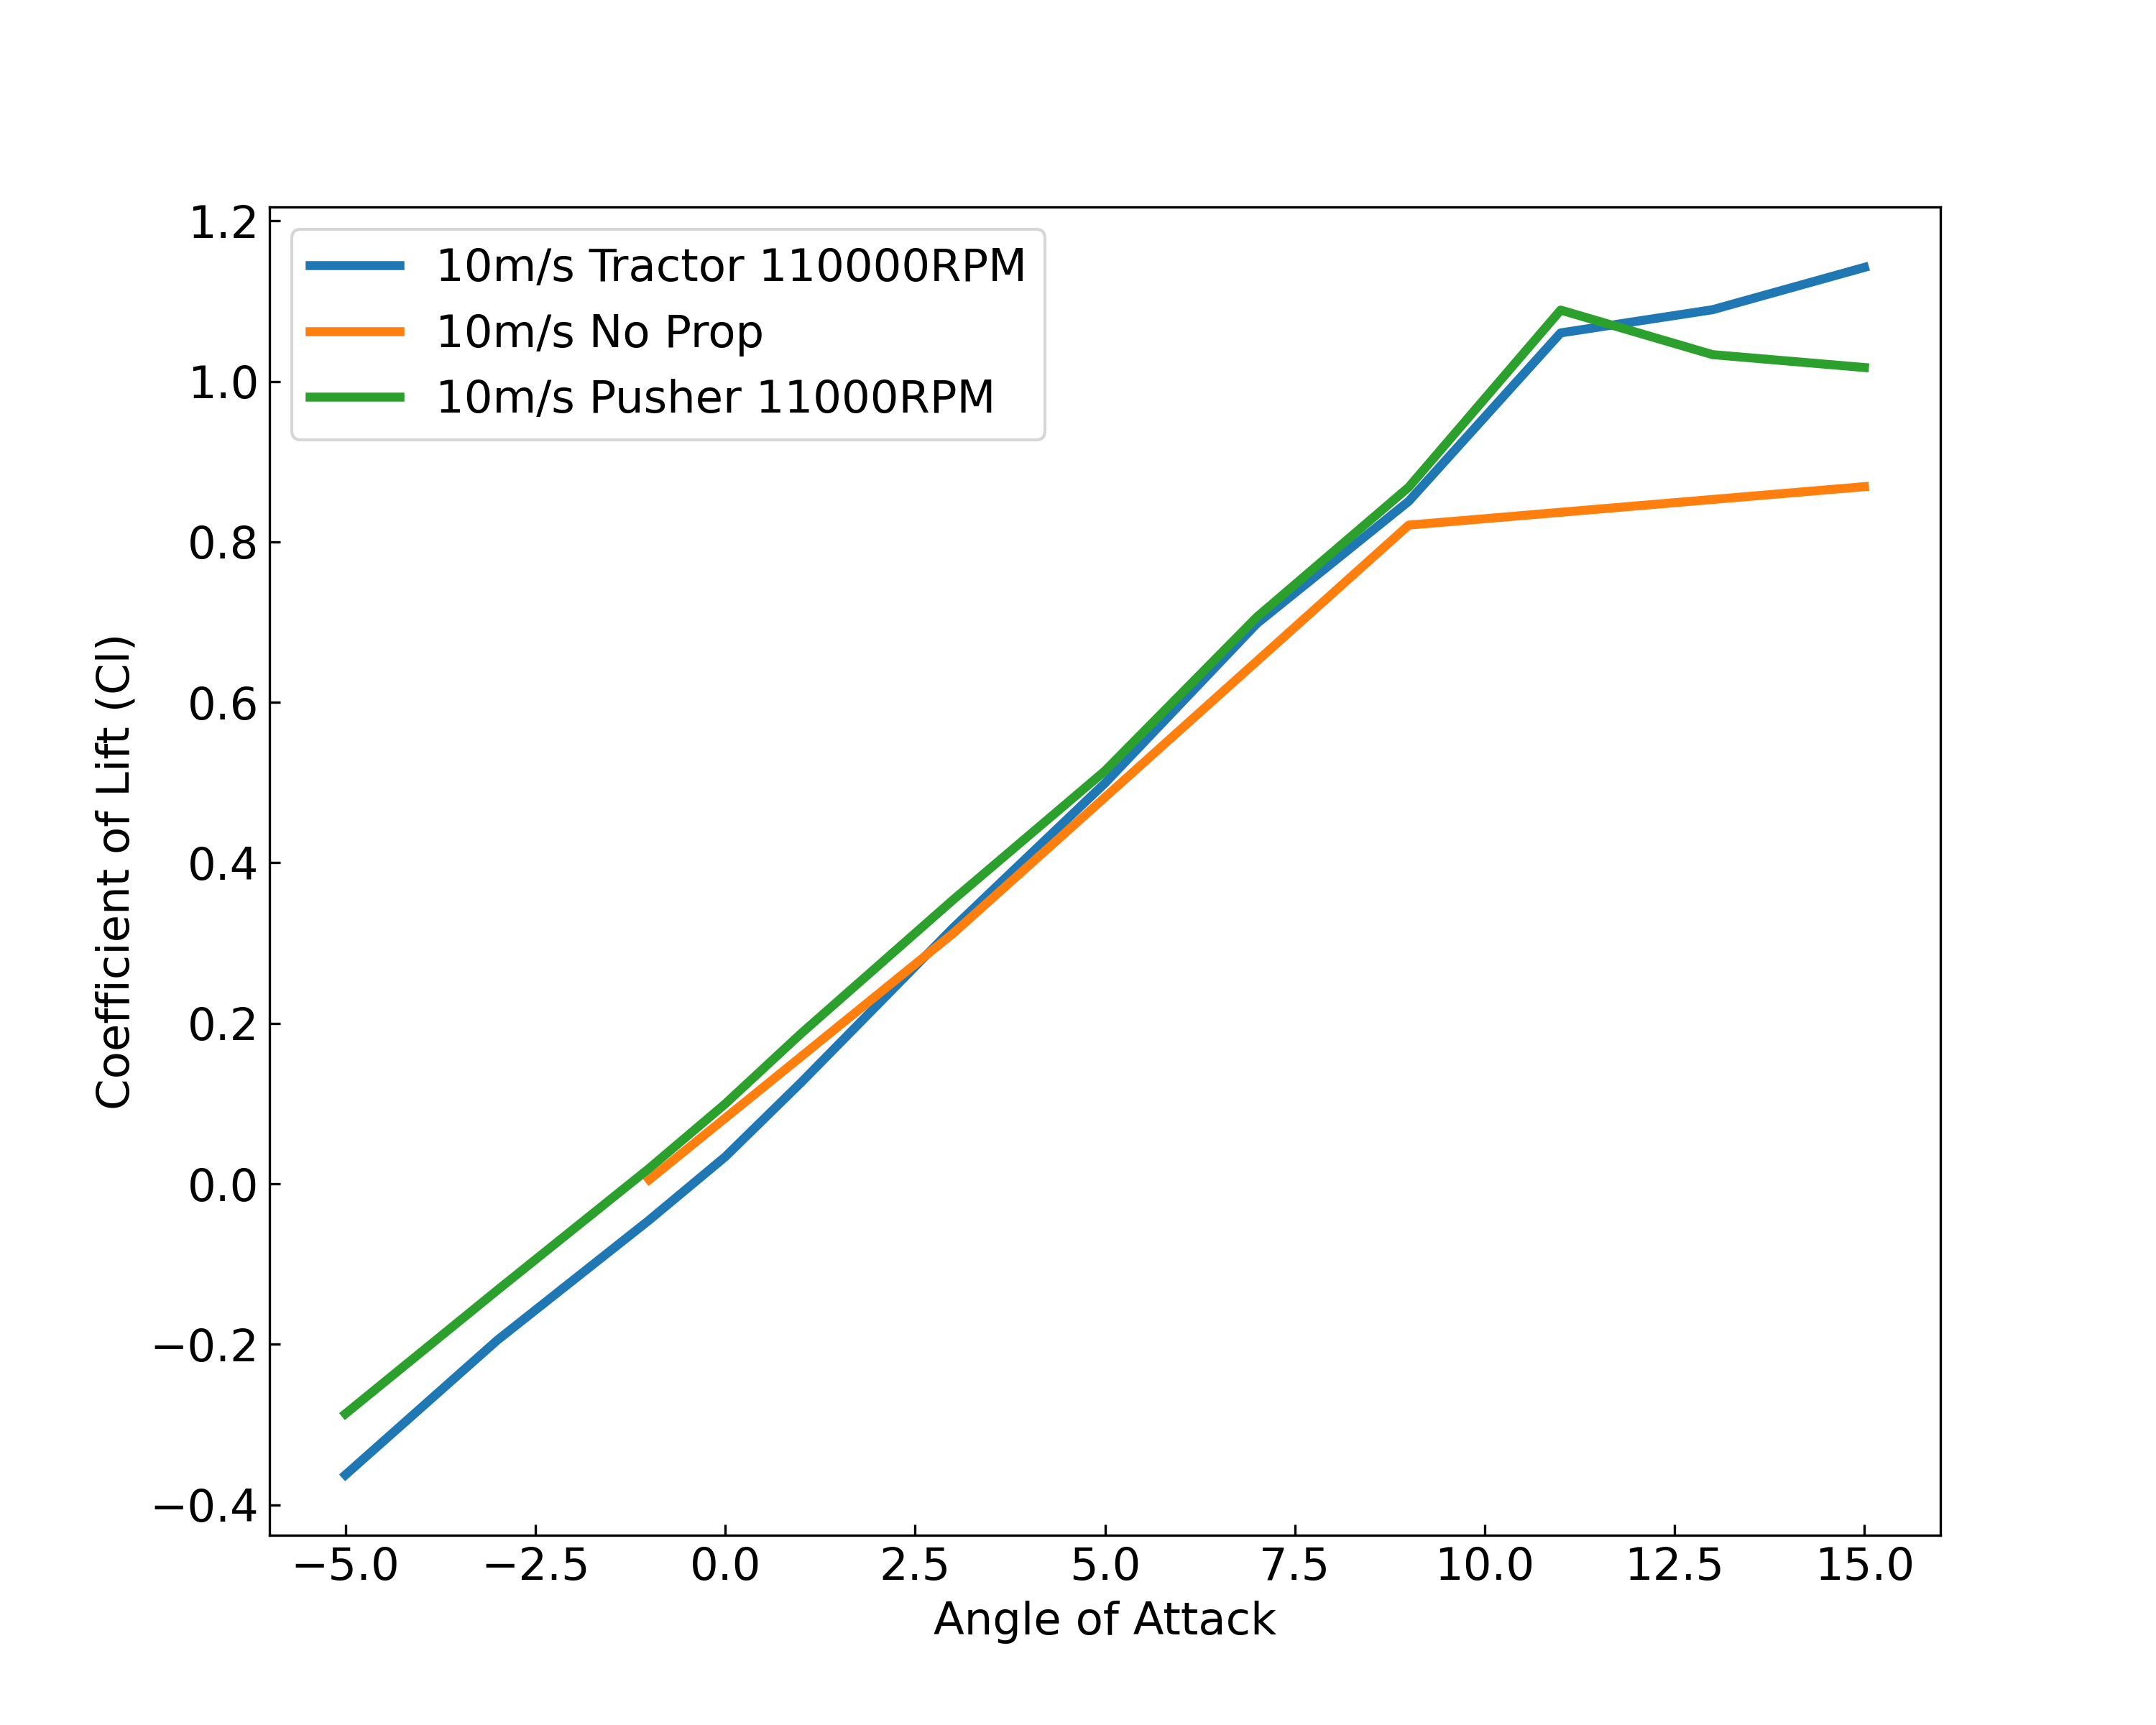
\includegraphics[width=\textwidth]{05_Results/Figs/Cl/10ms_110000RPM_Cl.png}
        \caption{Coefficient of lift at 10m/s airspeed and 11000RPM motor speed}
        \label{fig:Cl_10ms_11000}
    \end{subfigure}
    \begin{subfigure}[b]{0.467\textwidth}
        \centering
        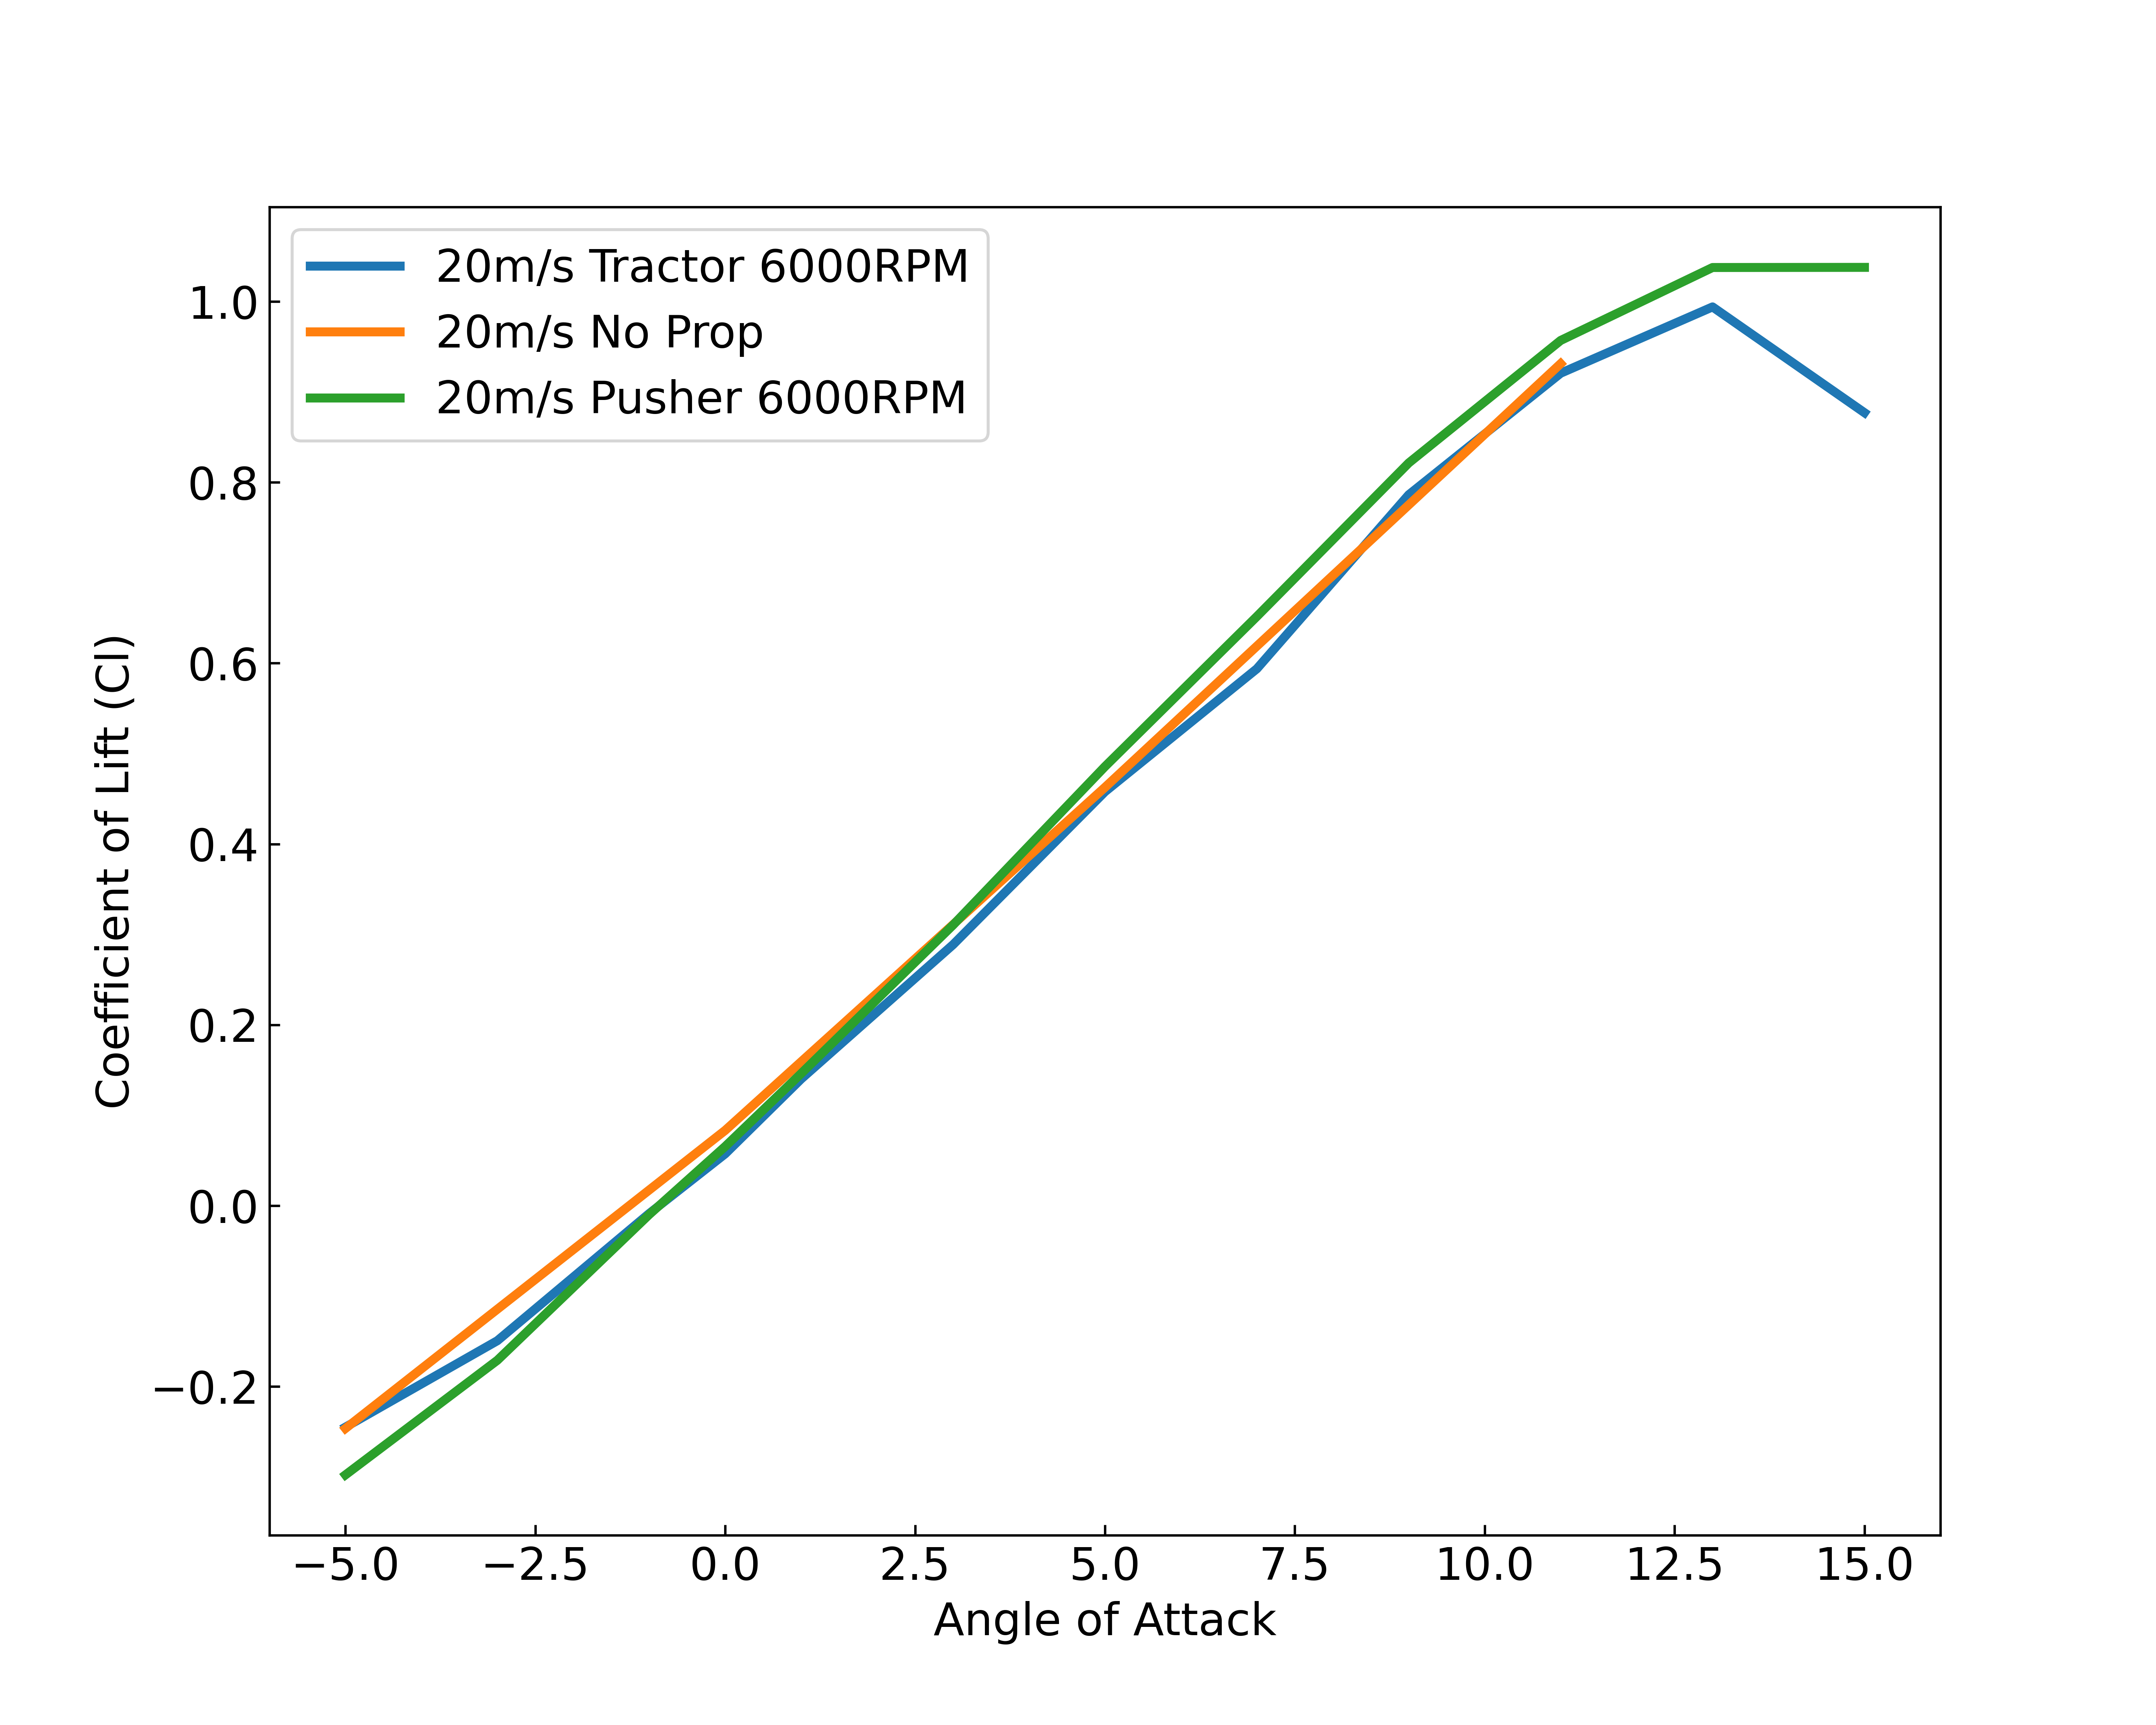
\includegraphics[width=\textwidth]{05_Results/Figs/Cl/20ms_6000RPM_Cl.png}
        \caption{Coefficient of lift at 20m/s airspeed and 6000RPM motor speed}
        \label{fig:Cl_20ms_6000}
    \end{subfigure}
    \begin{subfigure}[b]{0.467\textwidth}
        \centering
        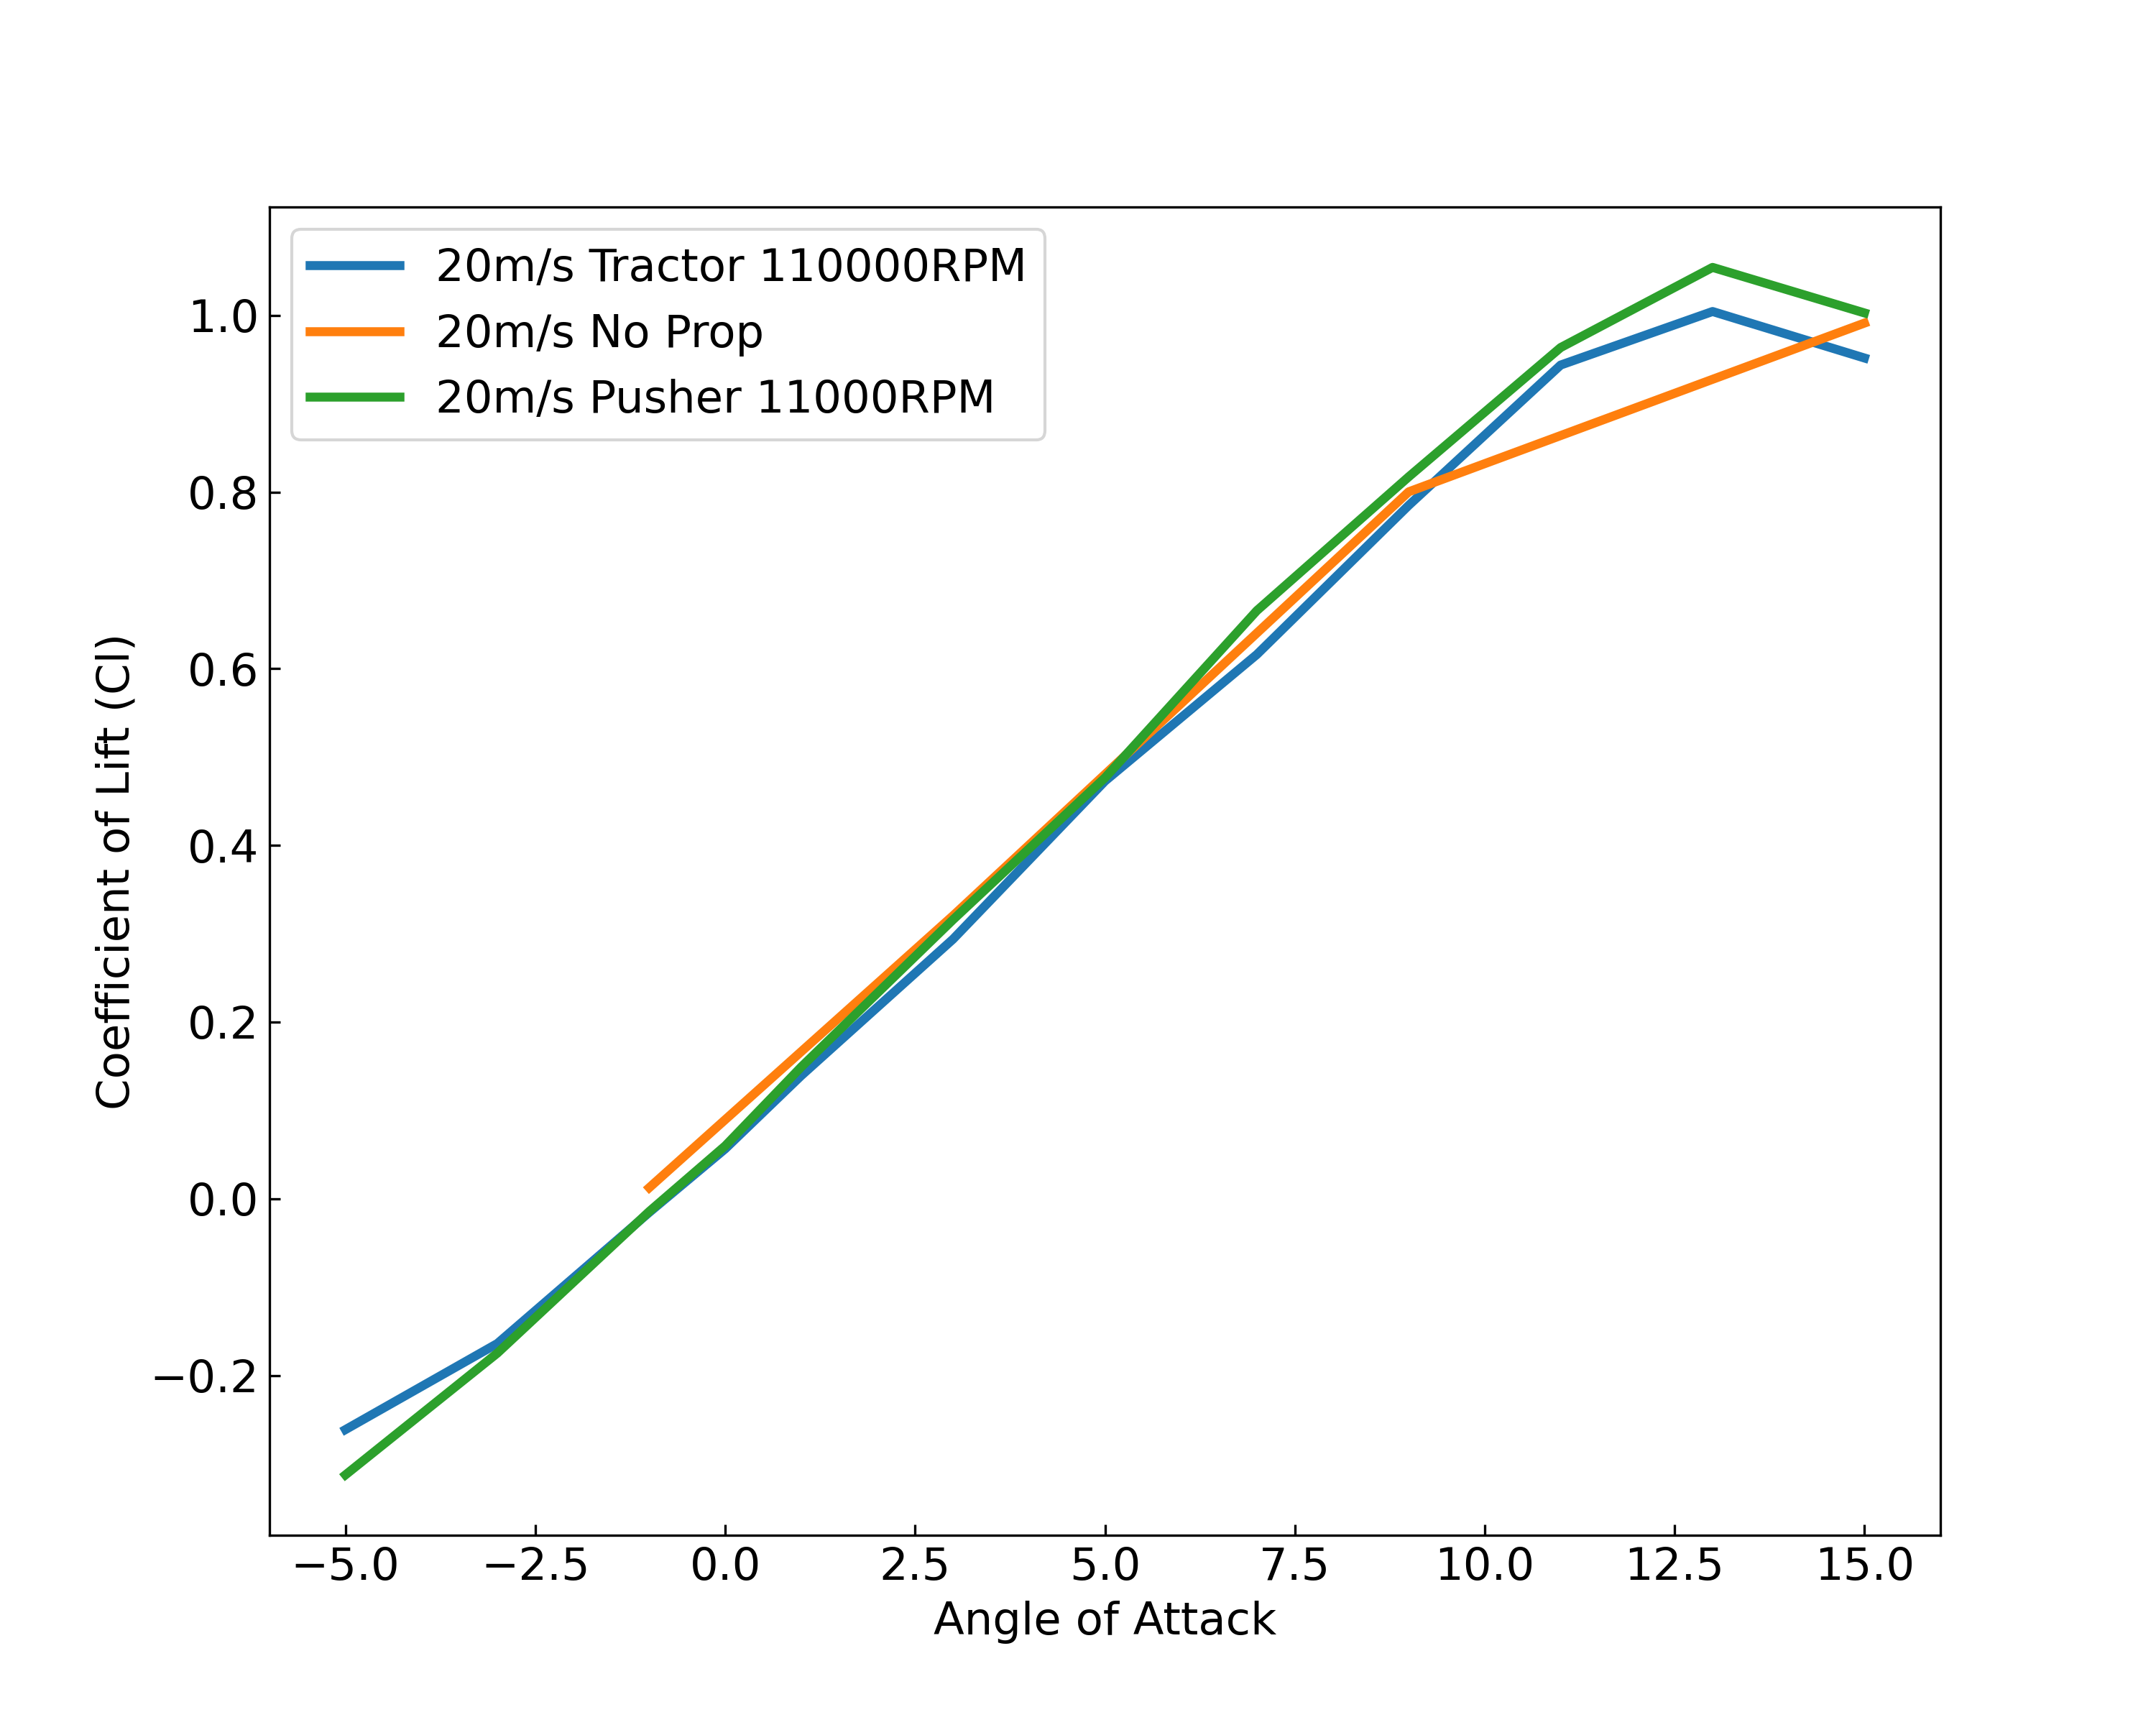
\includegraphics[width=\textwidth]{05_Results/Figs/Cl/20ms_110000RPM_Cl.png}
        \caption{Coefficient of lift at 20m/s airspeed and 11000RPM motor speed}
        \label{fig:Cl_20ms_11000}
    \end{subfigure}
    \caption{Coefficient of lift variation with various conditions for the pusher, tractor and no propeller configurations }
\end{figure}

\subsection{Aerodynamic Coefficient of Drag}
Figure \ref{fig:Cd_11000RPM} shows that as the wind tunnel airspeed increased, the drag coefficient shifted upwards for both the pusher and tractor configuration. The drag for both the tractor and puller configuration at 10m$s^{-1}$ airspeed is negative and shifts to positive value as the airspeed increases to 20m$s^{-1}$. This is due to the thrust produced by the propeller decreasing as the airspeed increases for both the tractor and puller configurations. The drag curve shifts into negative values for the tractor and puller configurations due to the thrust produced by the propeller. As the overall drag is a measure of the thrust minus drag, the overall drag becomes negative, shifting the coefficient of drag curve into negative values. As the airspeed increases, the drag coefficient is also seen to increase for the pusher and tractor configuration due to an increase in drag for the overall model with increasing airspeed. This shifts the coefficient of drag curves upwards as the airspeed increases. The highest drag coefficient occurred when no propeller operated on the MAV model. Ananda concluded that for tractor configuration propeller-wing set up in a low-speed wind tunnel, the flow transitions to turbulent flow earlier. This reduces the drag and increases the lift-to-drag ratio \cite{Ananda2018}. This shows a discrepancy with the results seen in this study. However, Ananda's setup involved a motor being mounted in front of the wing with no direct attachment; hence, the forces are not directly applied to the wing \cite{Ananda2018}. When no propeller is added, no significant changes are seen in airspeed for the drag coefficient. The tractor configuration, in general, produces less drag than the pusher configuration; hence, the drag coefficient is lower for the tractor configuration. This is most clearly seen at 20m$s^{-1}$ in Figure \ref{fig:Cd_11000RPM}. 




\begin{figure}[H]
    \centering
    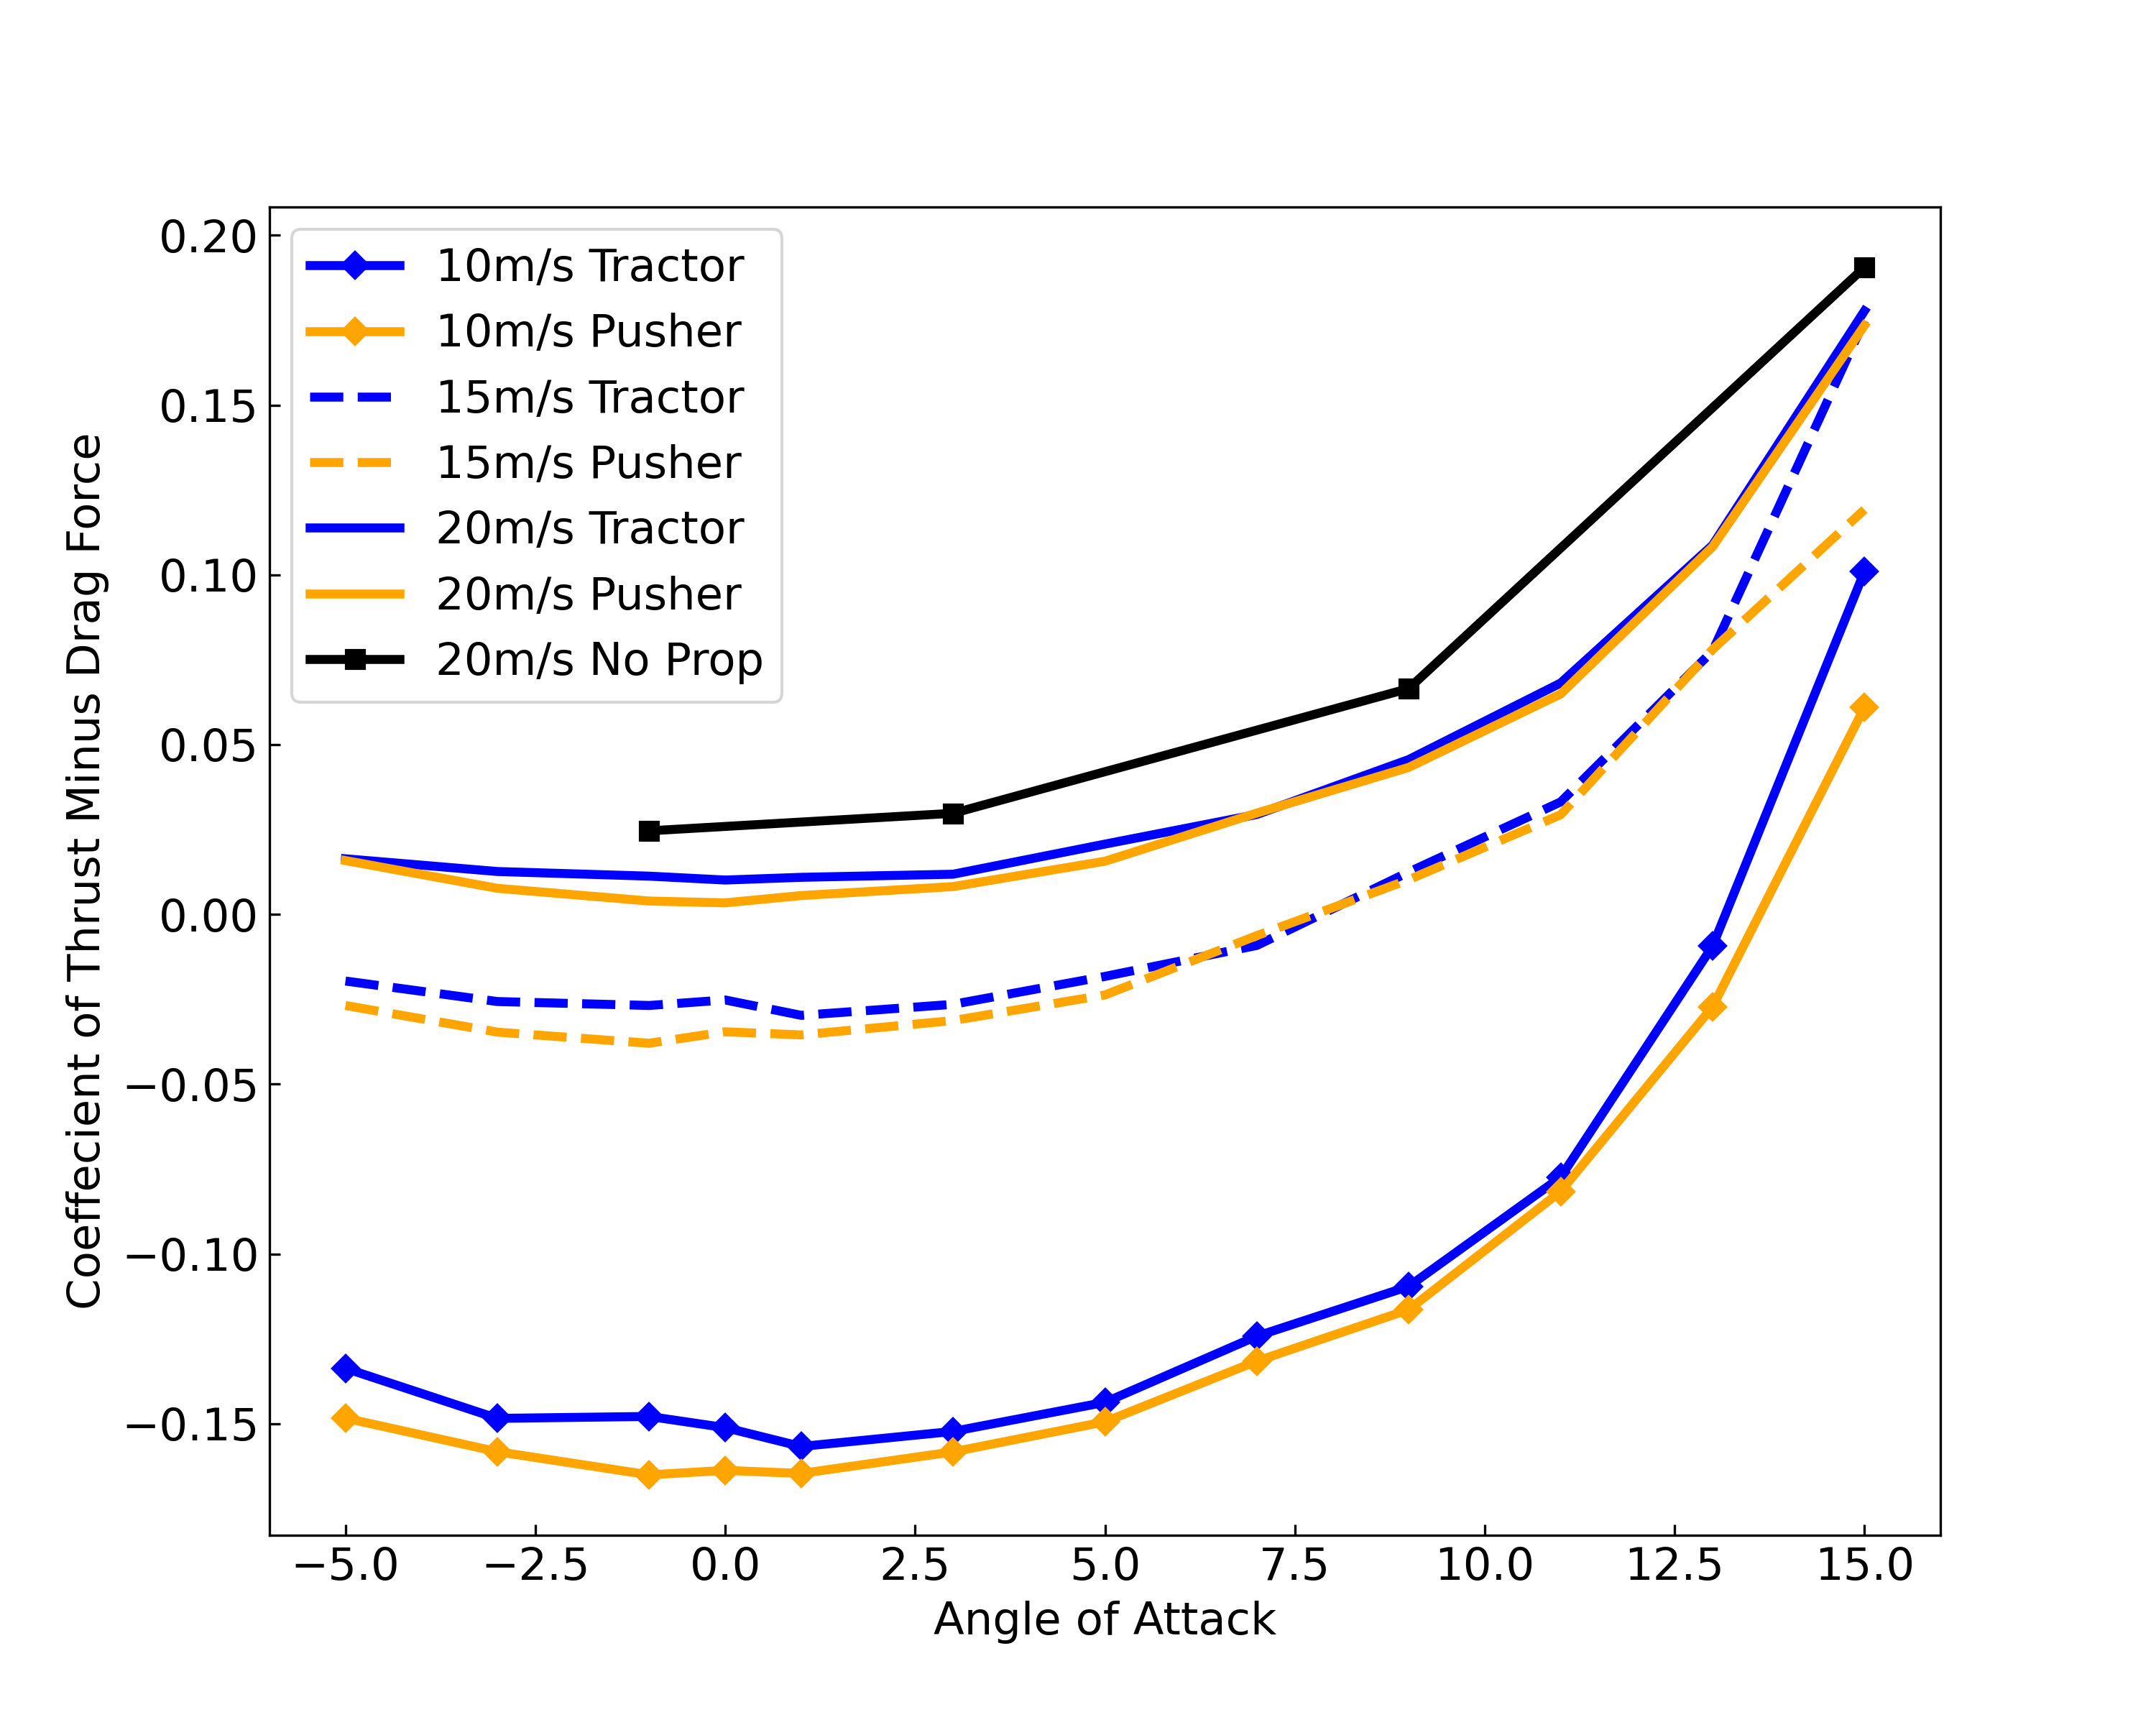
\includegraphics[scale = 0.7]{05_Results/Figs/Cd/110000RPM_Cd.png}
    \caption{Coefficient of drag variation at 11000RPM motor speed for the tractor, pusher and no propeller configurations}
    \label{fig:Cd_11000RPM}
\end{figure}

Figure \ref{fig:Cd_20ms} shows minimal differences between the pusher and tractor configurations. The addition of the propeller increases the drag coefficient at 6000RPM and shows that the propellers do not produce enough thrust to overcome the drag at 20m$s^{-1}$. As the motor speed increases to 11000RPM, there is a significant drop in the drag coefficient for both the tractor and pusher configuration, showing that the thrust produced can overcome drag at 11000RPM. 


\begin{figure}[H]
    \centering
    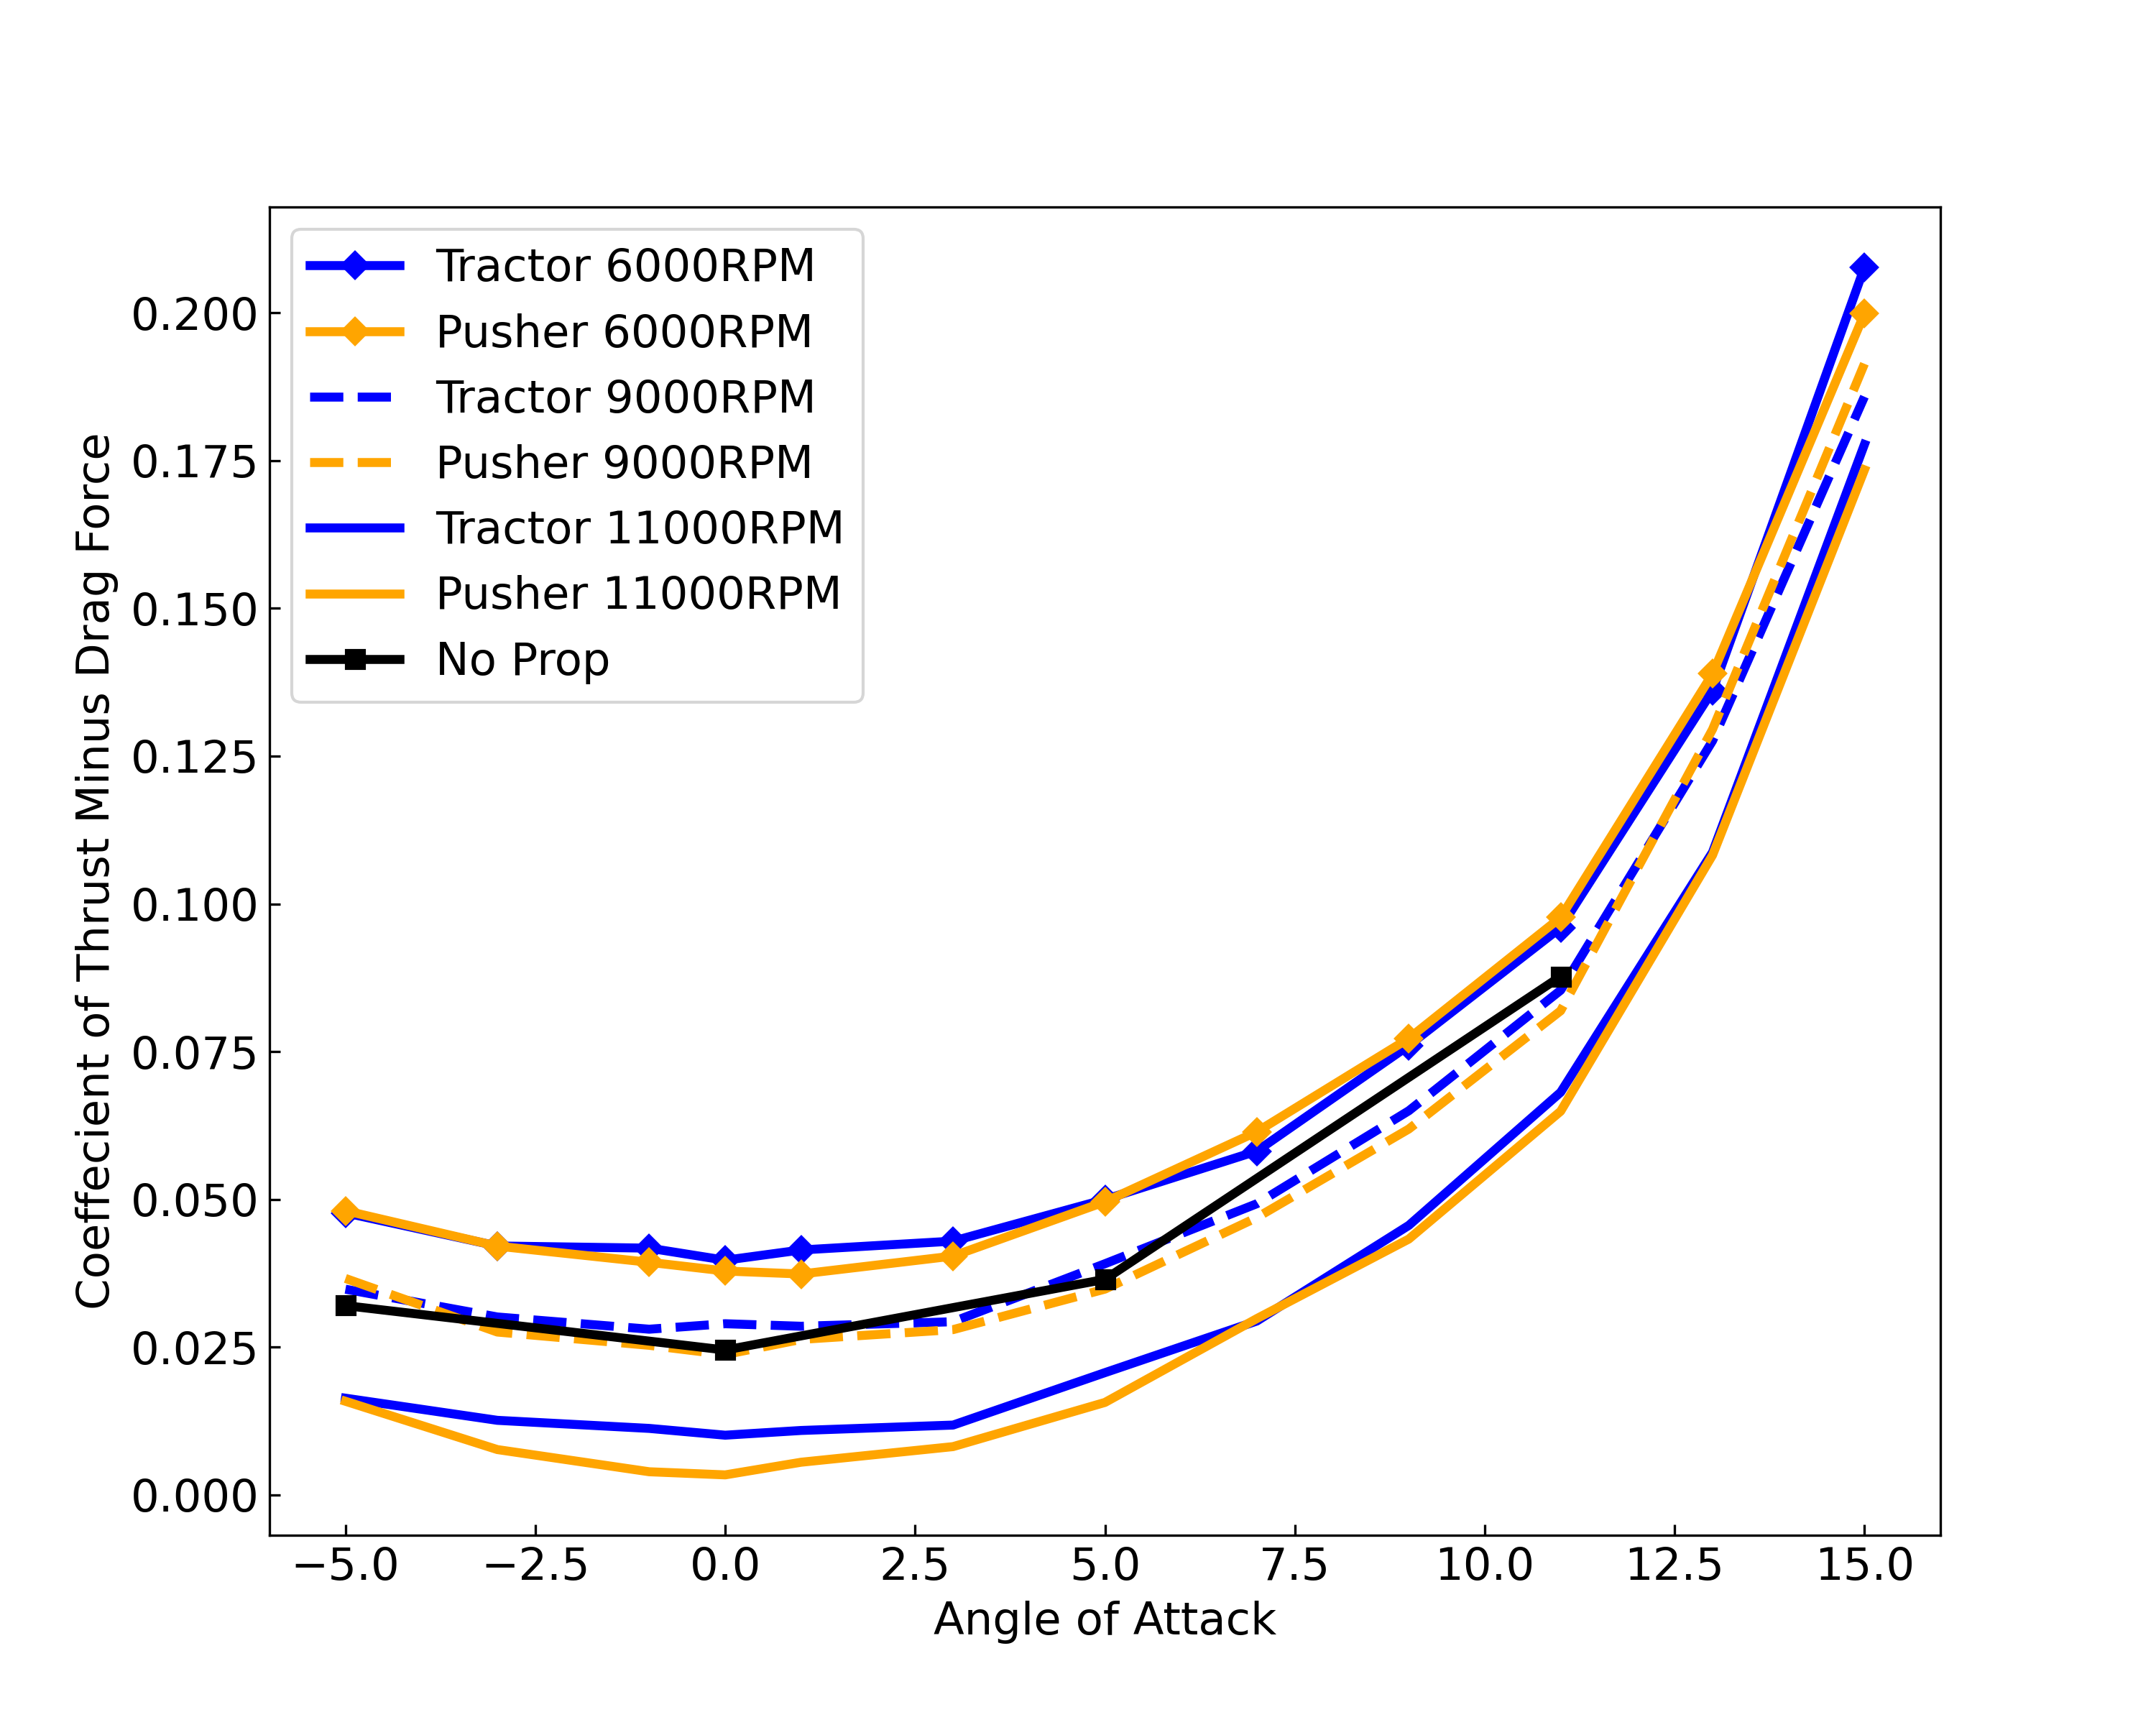
\includegraphics[scale = 0.7]{05_Results/Figs/Cd/20ms_Cd.png}
    \caption{Coefficient of drag variation at 20ms airspeed for the tractor, pusher and no propeller configuration}
    \label{fig:Cd_20ms}
\end{figure}



\subsection{Pitching Moment Coefficient}

Figures \Cref{fig:Cm_10ms_6000} to \Cref{fig:Cm_20ms_11000} show that for all cases, the pitching moment of the MAV model decreases as the angle of attack increases. This leads to a stable MAV in all cases as the longitudinal stability is maintained due to the pitching down motion of the MAV as the \acrshort{AoA} increases. Figures \Cref{fig:Cm_10ms_6000} to \Cref{fig:Cm_20ms_11000} also show that as the motor speed increases from 6000RPM to 11000RPM, the tractor configuration experienced a decrease in pitching coefficient compared with the no propeller model up until stall at approximately 12$^\circ$ AoA. The pusher configuration experienced an increase in the pitching moment compared with the no-propeller model. This shows that as the airspeed and propeller speed increase, the tractor configuration becomes less stable, while the pusher configuration becomes more stable. Increasing the airspeed decreased the pitching moment for all motor speeds.

\begin{figure}[H]
    \centering
    \begin{subfigure}[b]{0.467\textwidth}
        \centering
        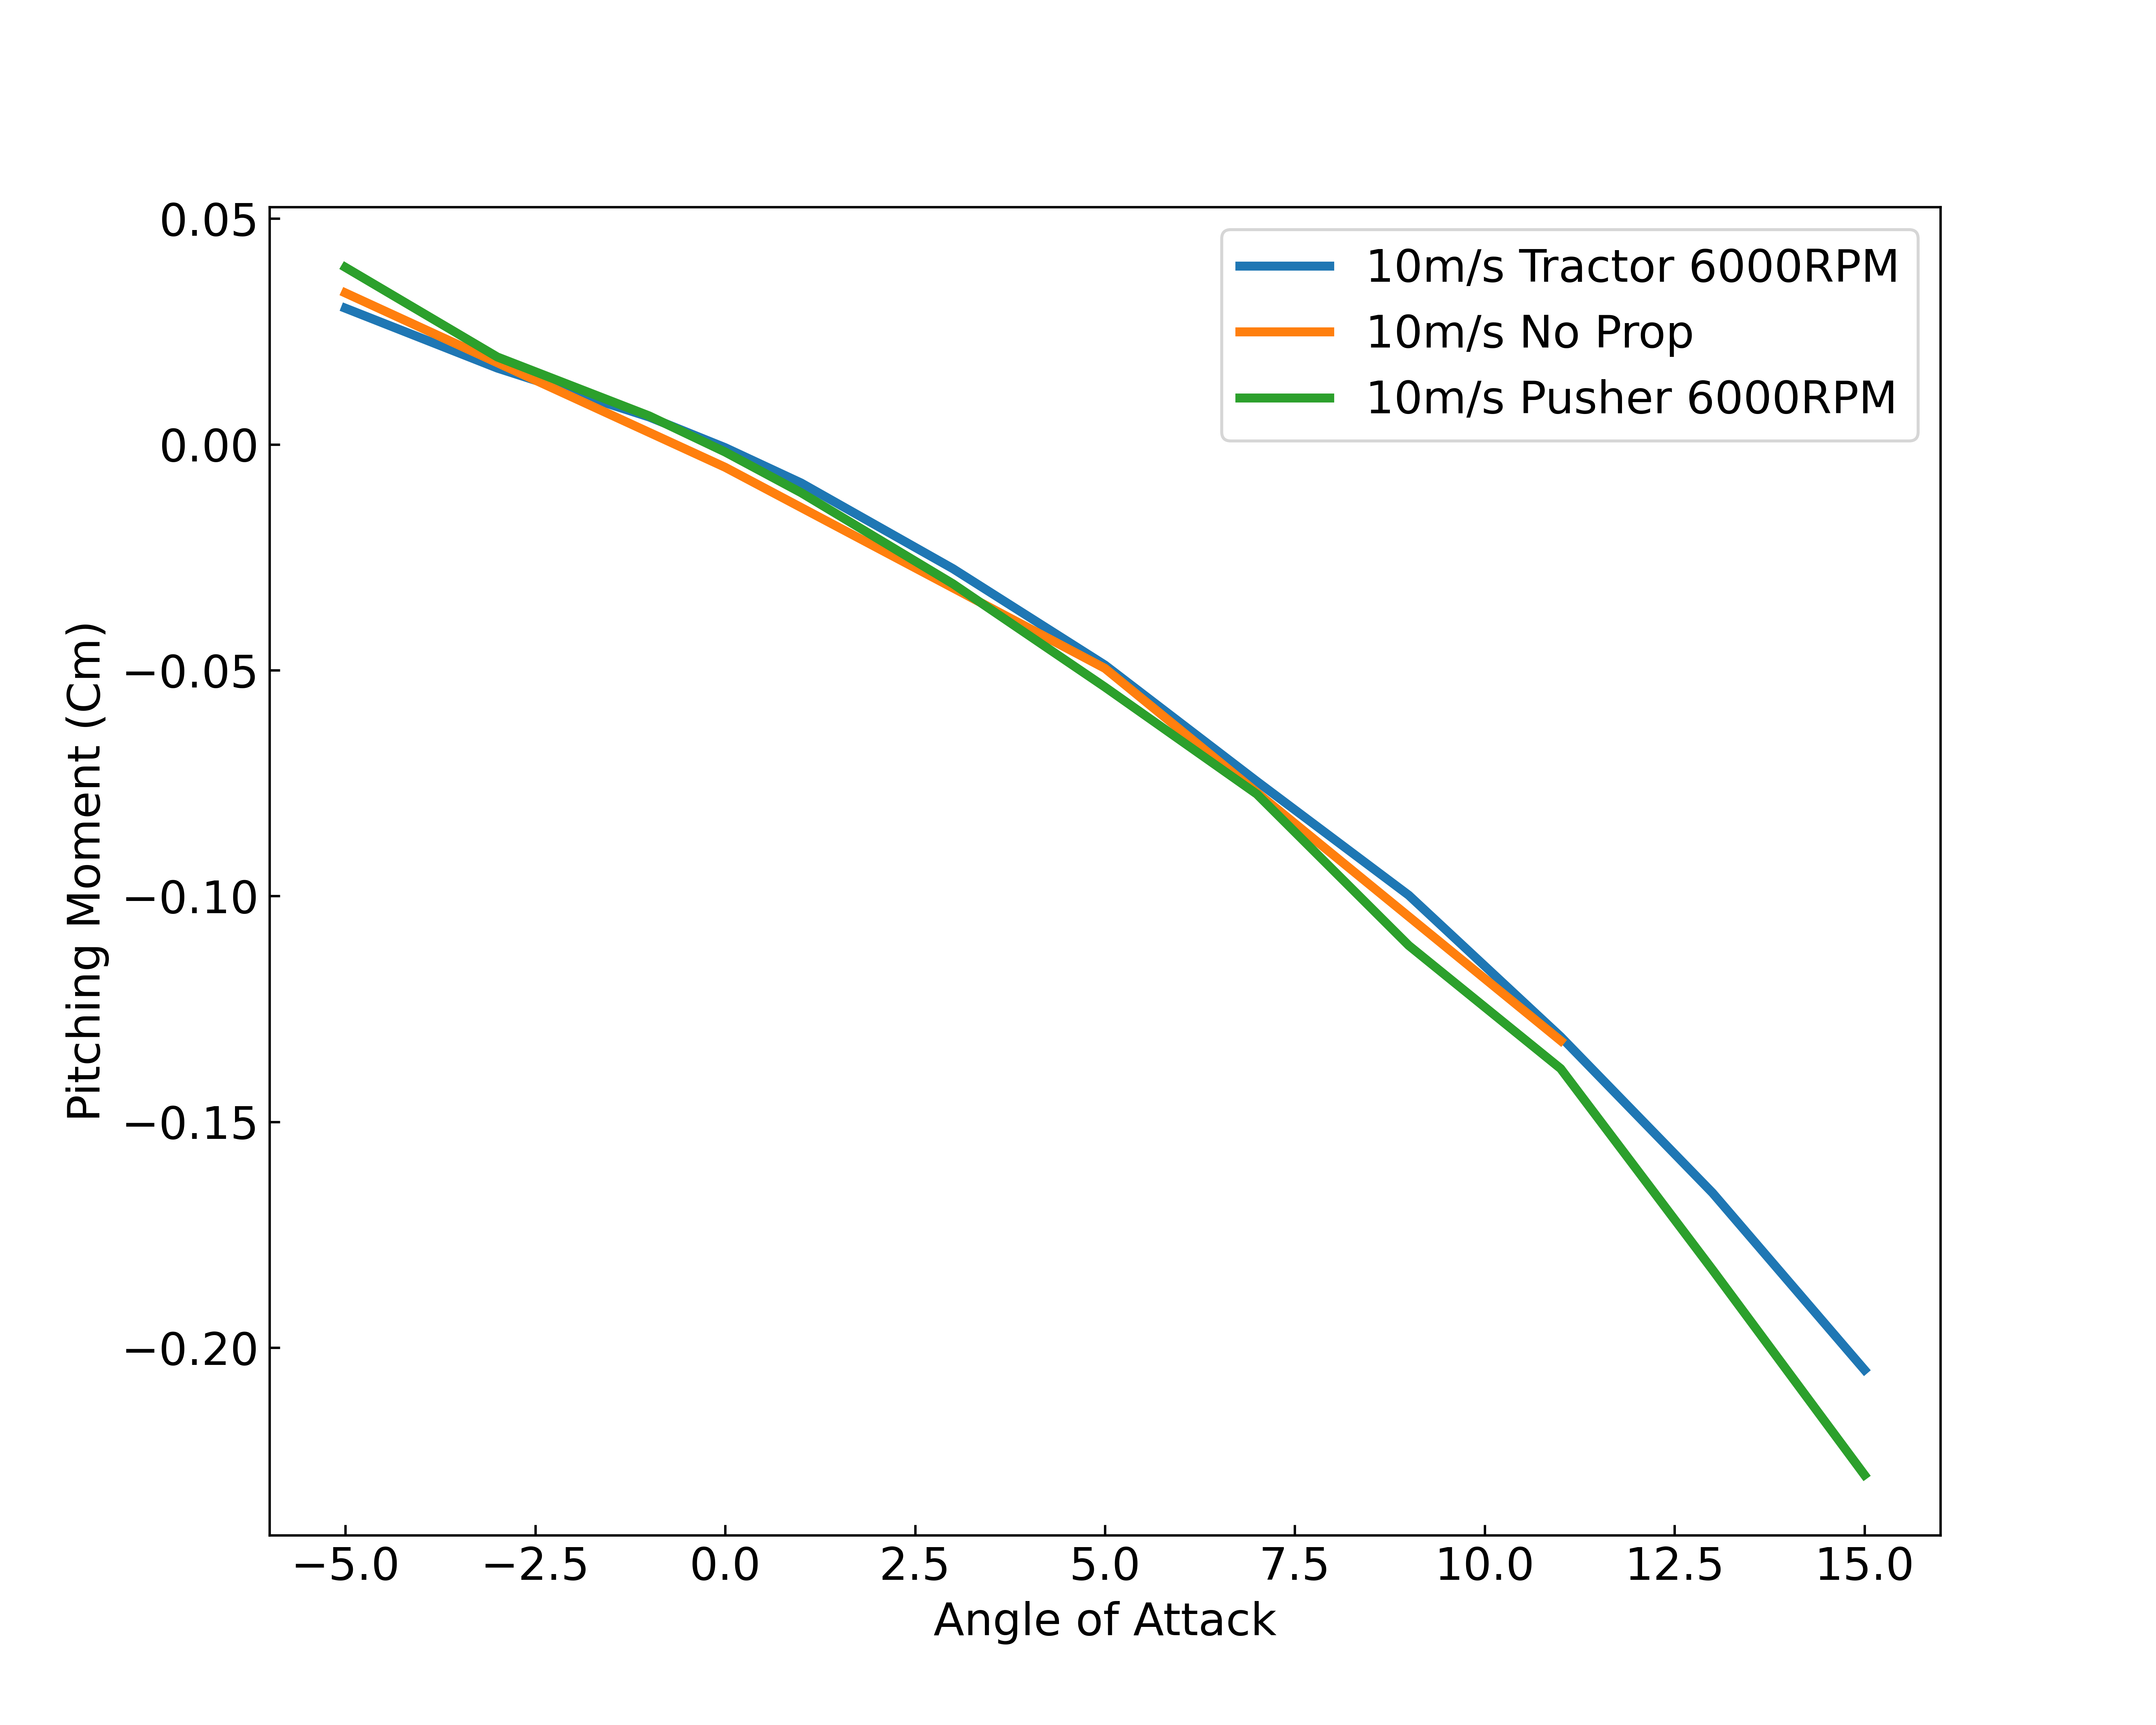
\includegraphics[width=\textwidth]{05_Results/Figs/Cm/10ms_6000RPM_Cm.png}
        \caption{Pitching Moment Coefficient at 10m/s airspeed and 6000RPM motor speed}
        \label{fig:Cm_10ms_6000}
    \end{subfigure}
    \begin{subfigure}[b]{0.467\textwidth}
        \centering
        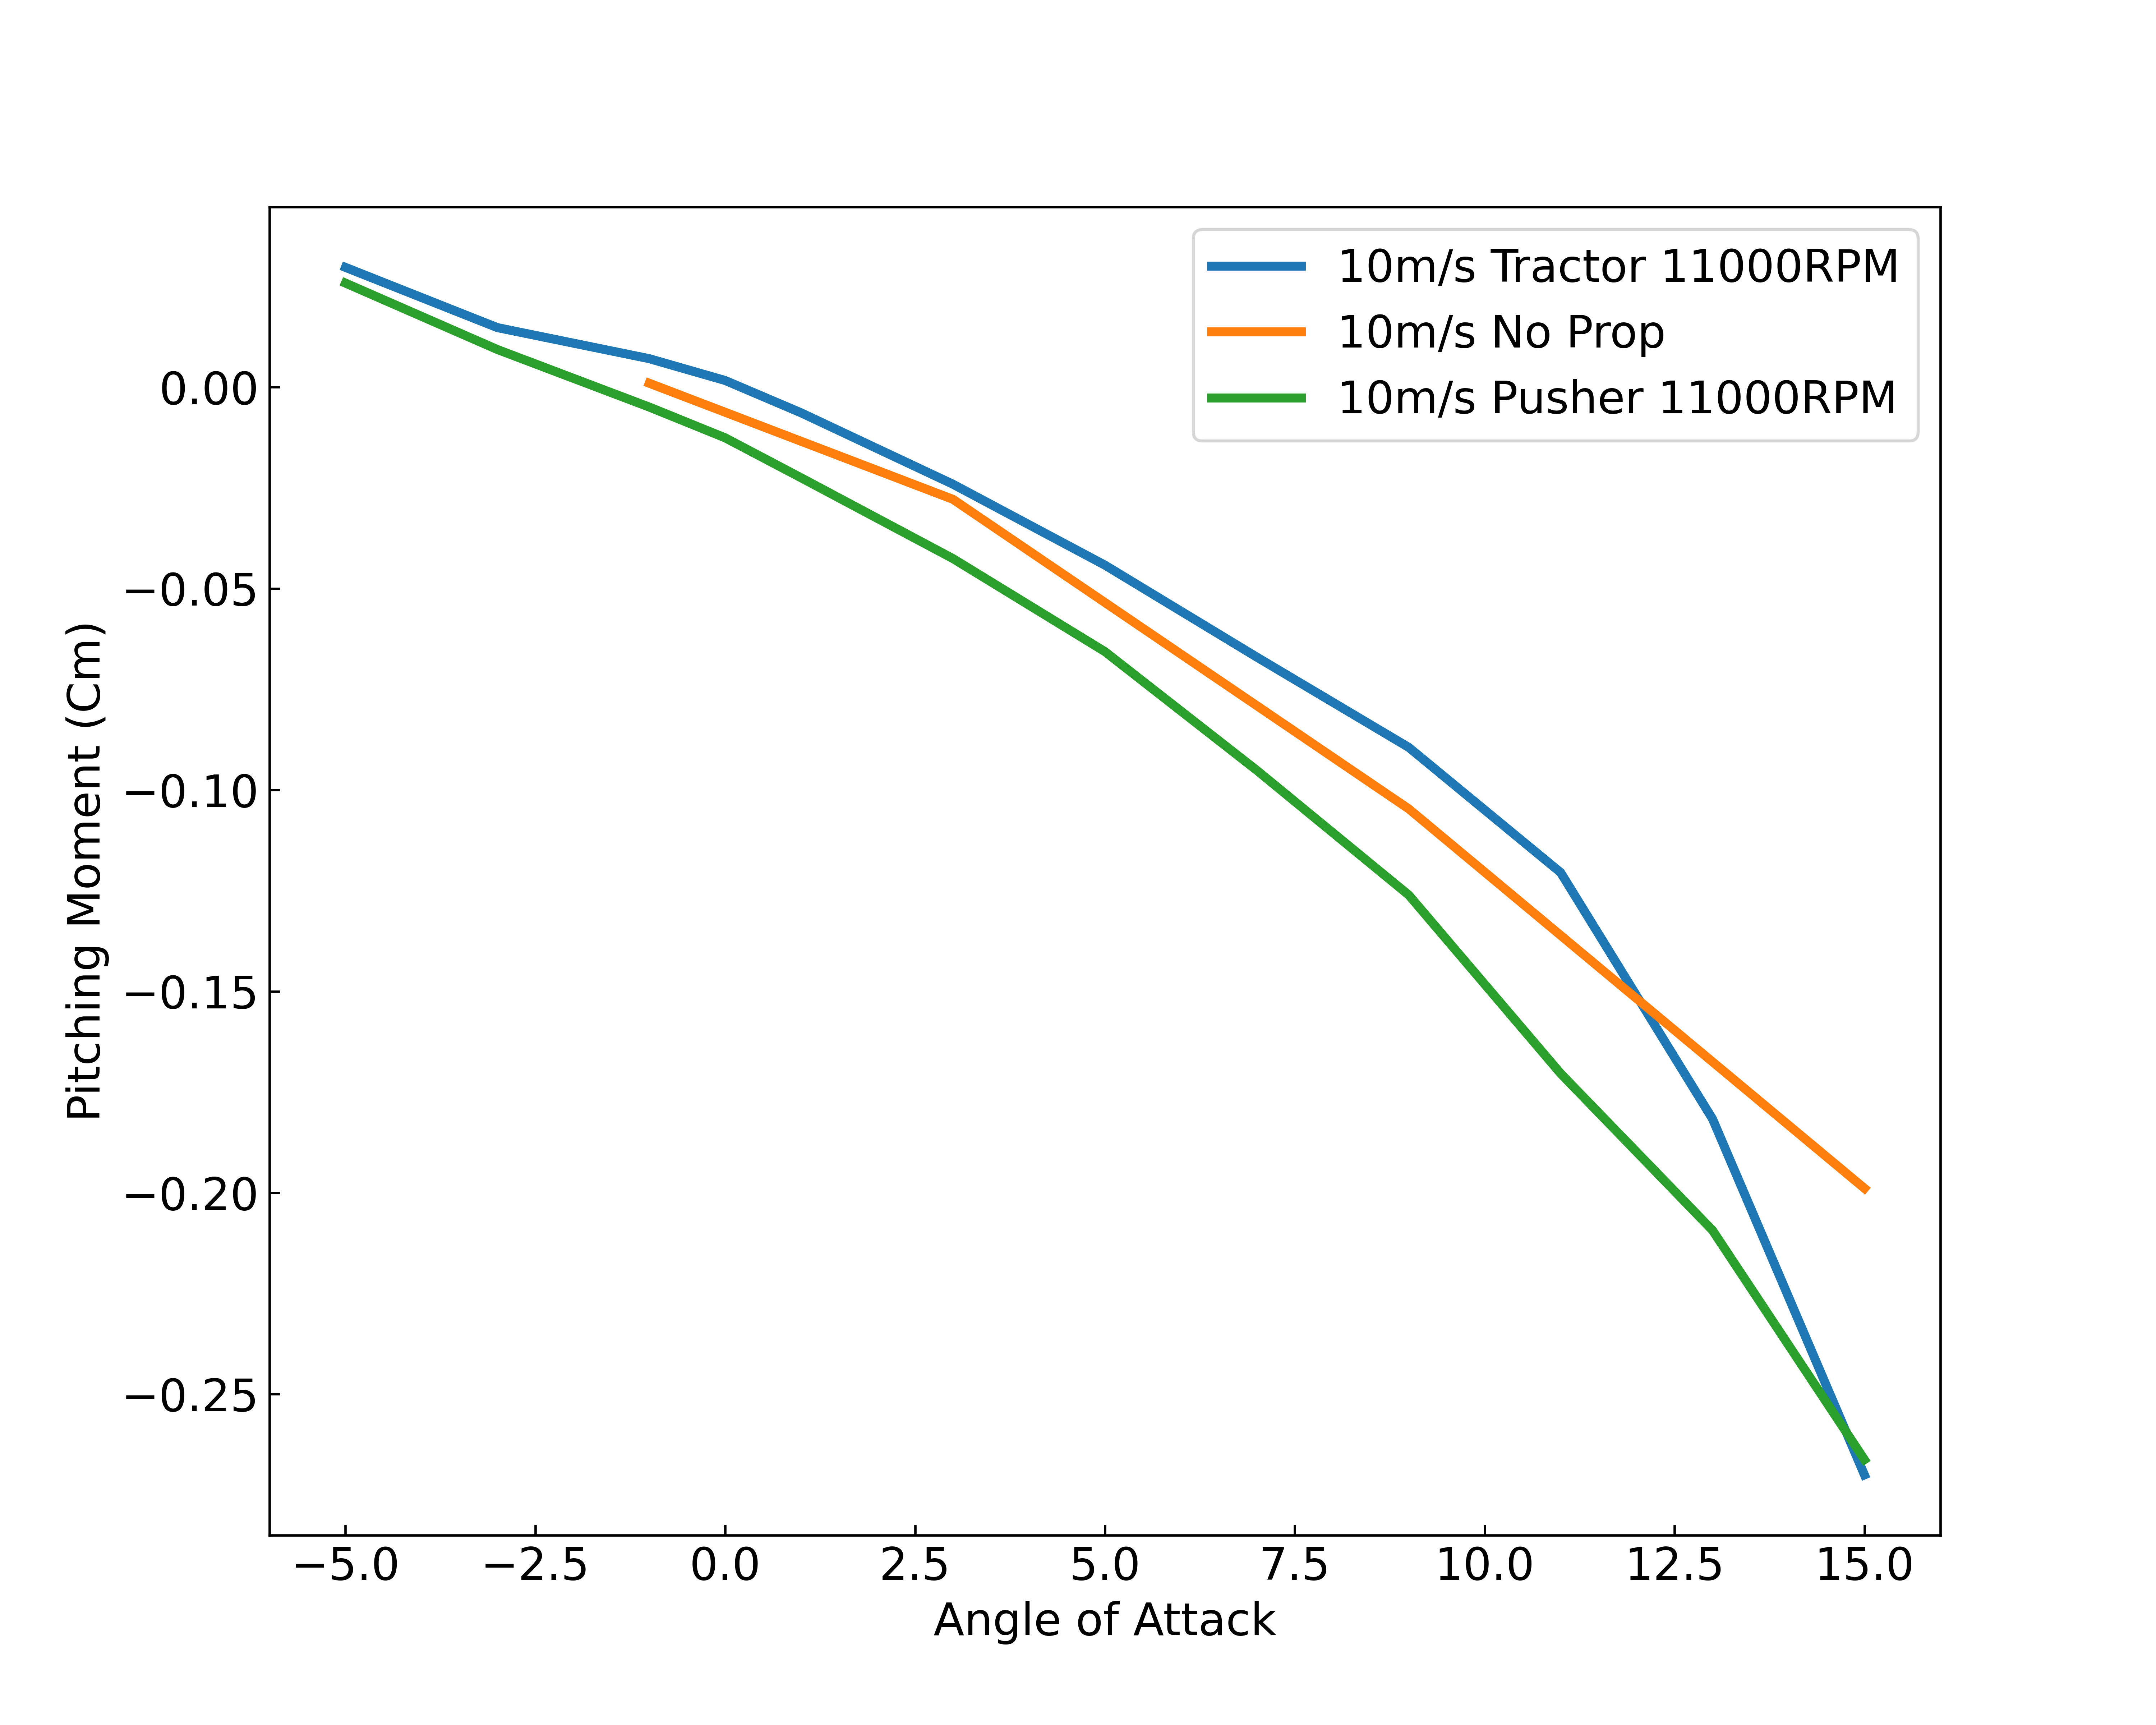
\includegraphics[width=\textwidth]{05_Results/Figs/Cm/10ms_11000RPM_Cm.png}
        \caption{Pitching Moment Coefficient at 10m/s airspeed and 11000RPM motor speed}
        \label{fig:Cm_10ms_11000}
    \end{subfigure}
    \begin{subfigure}[b]{0.467\textwidth}
        \centering
        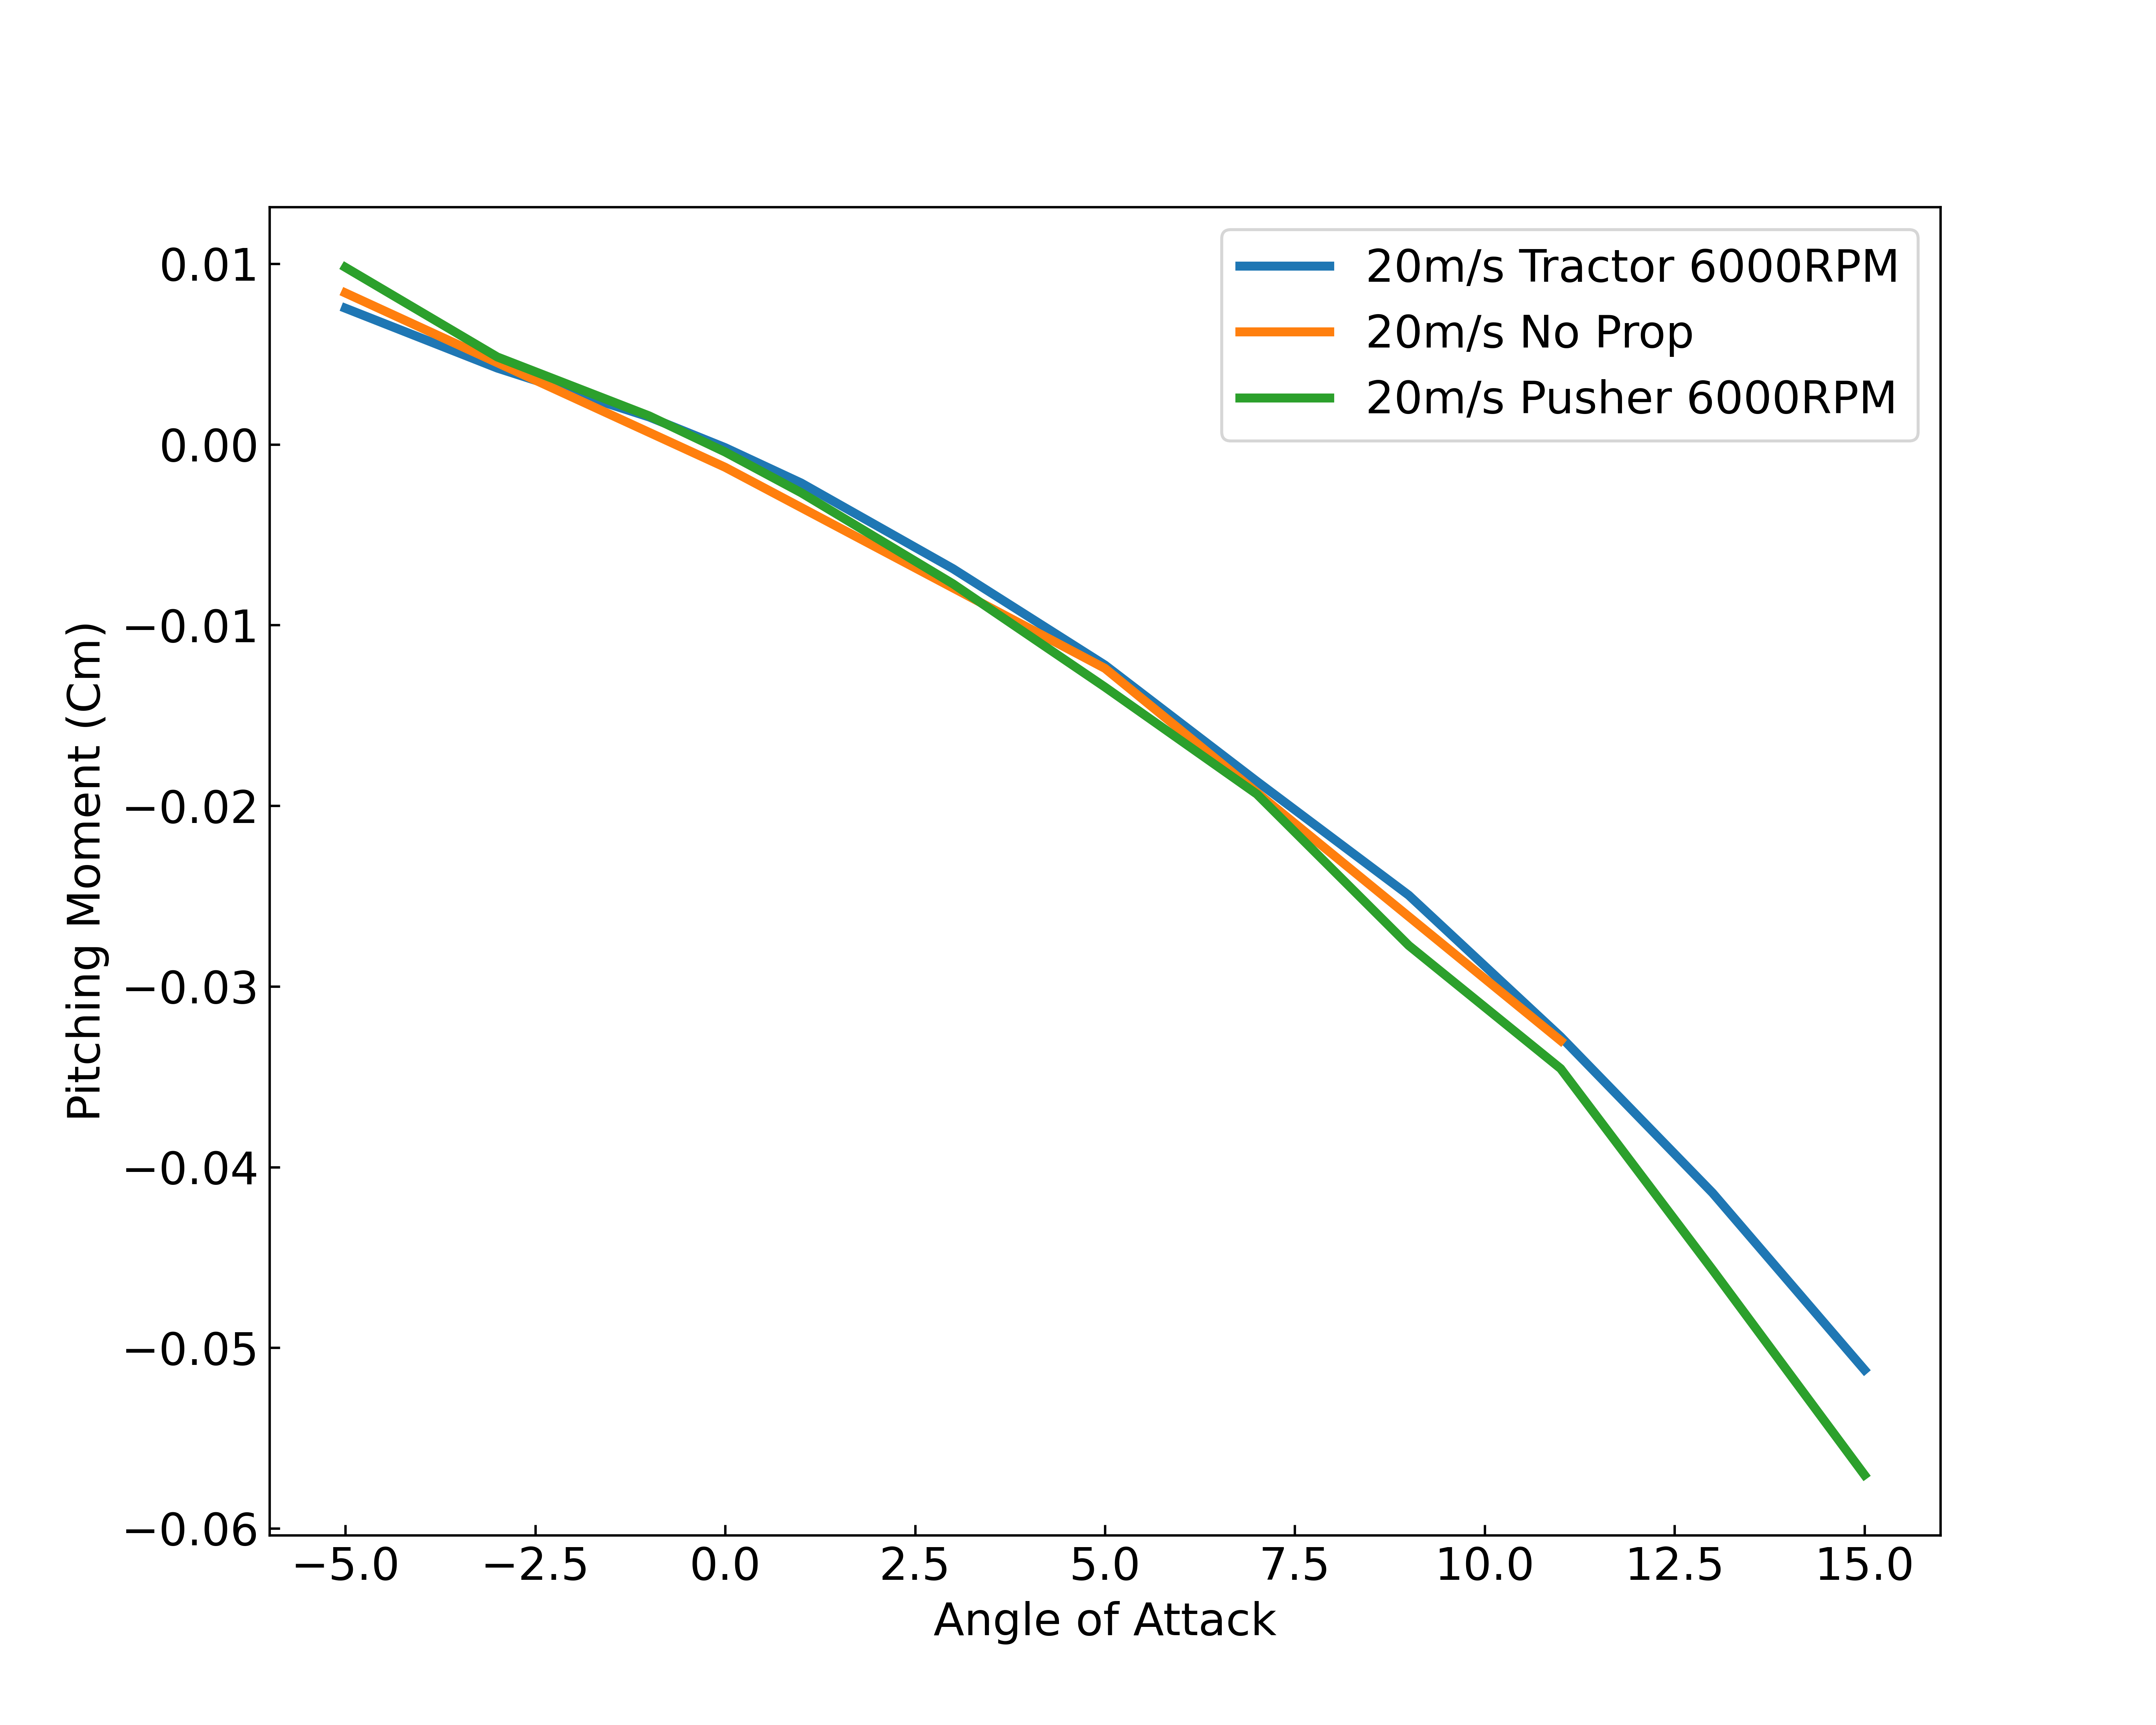
\includegraphics[width=\textwidth]{05_Results/Figs/Cm/20ms_6000RPM_Cm.png}
        \caption{Pitching Moment Coefficient at 20m/s airspeed and 6000RPM motor speed}
        \label{fig:Cm_20ms_6000}
    \end{subfigure}
    \begin{subfigure}[b]{0.467\textwidth}
        \centering
        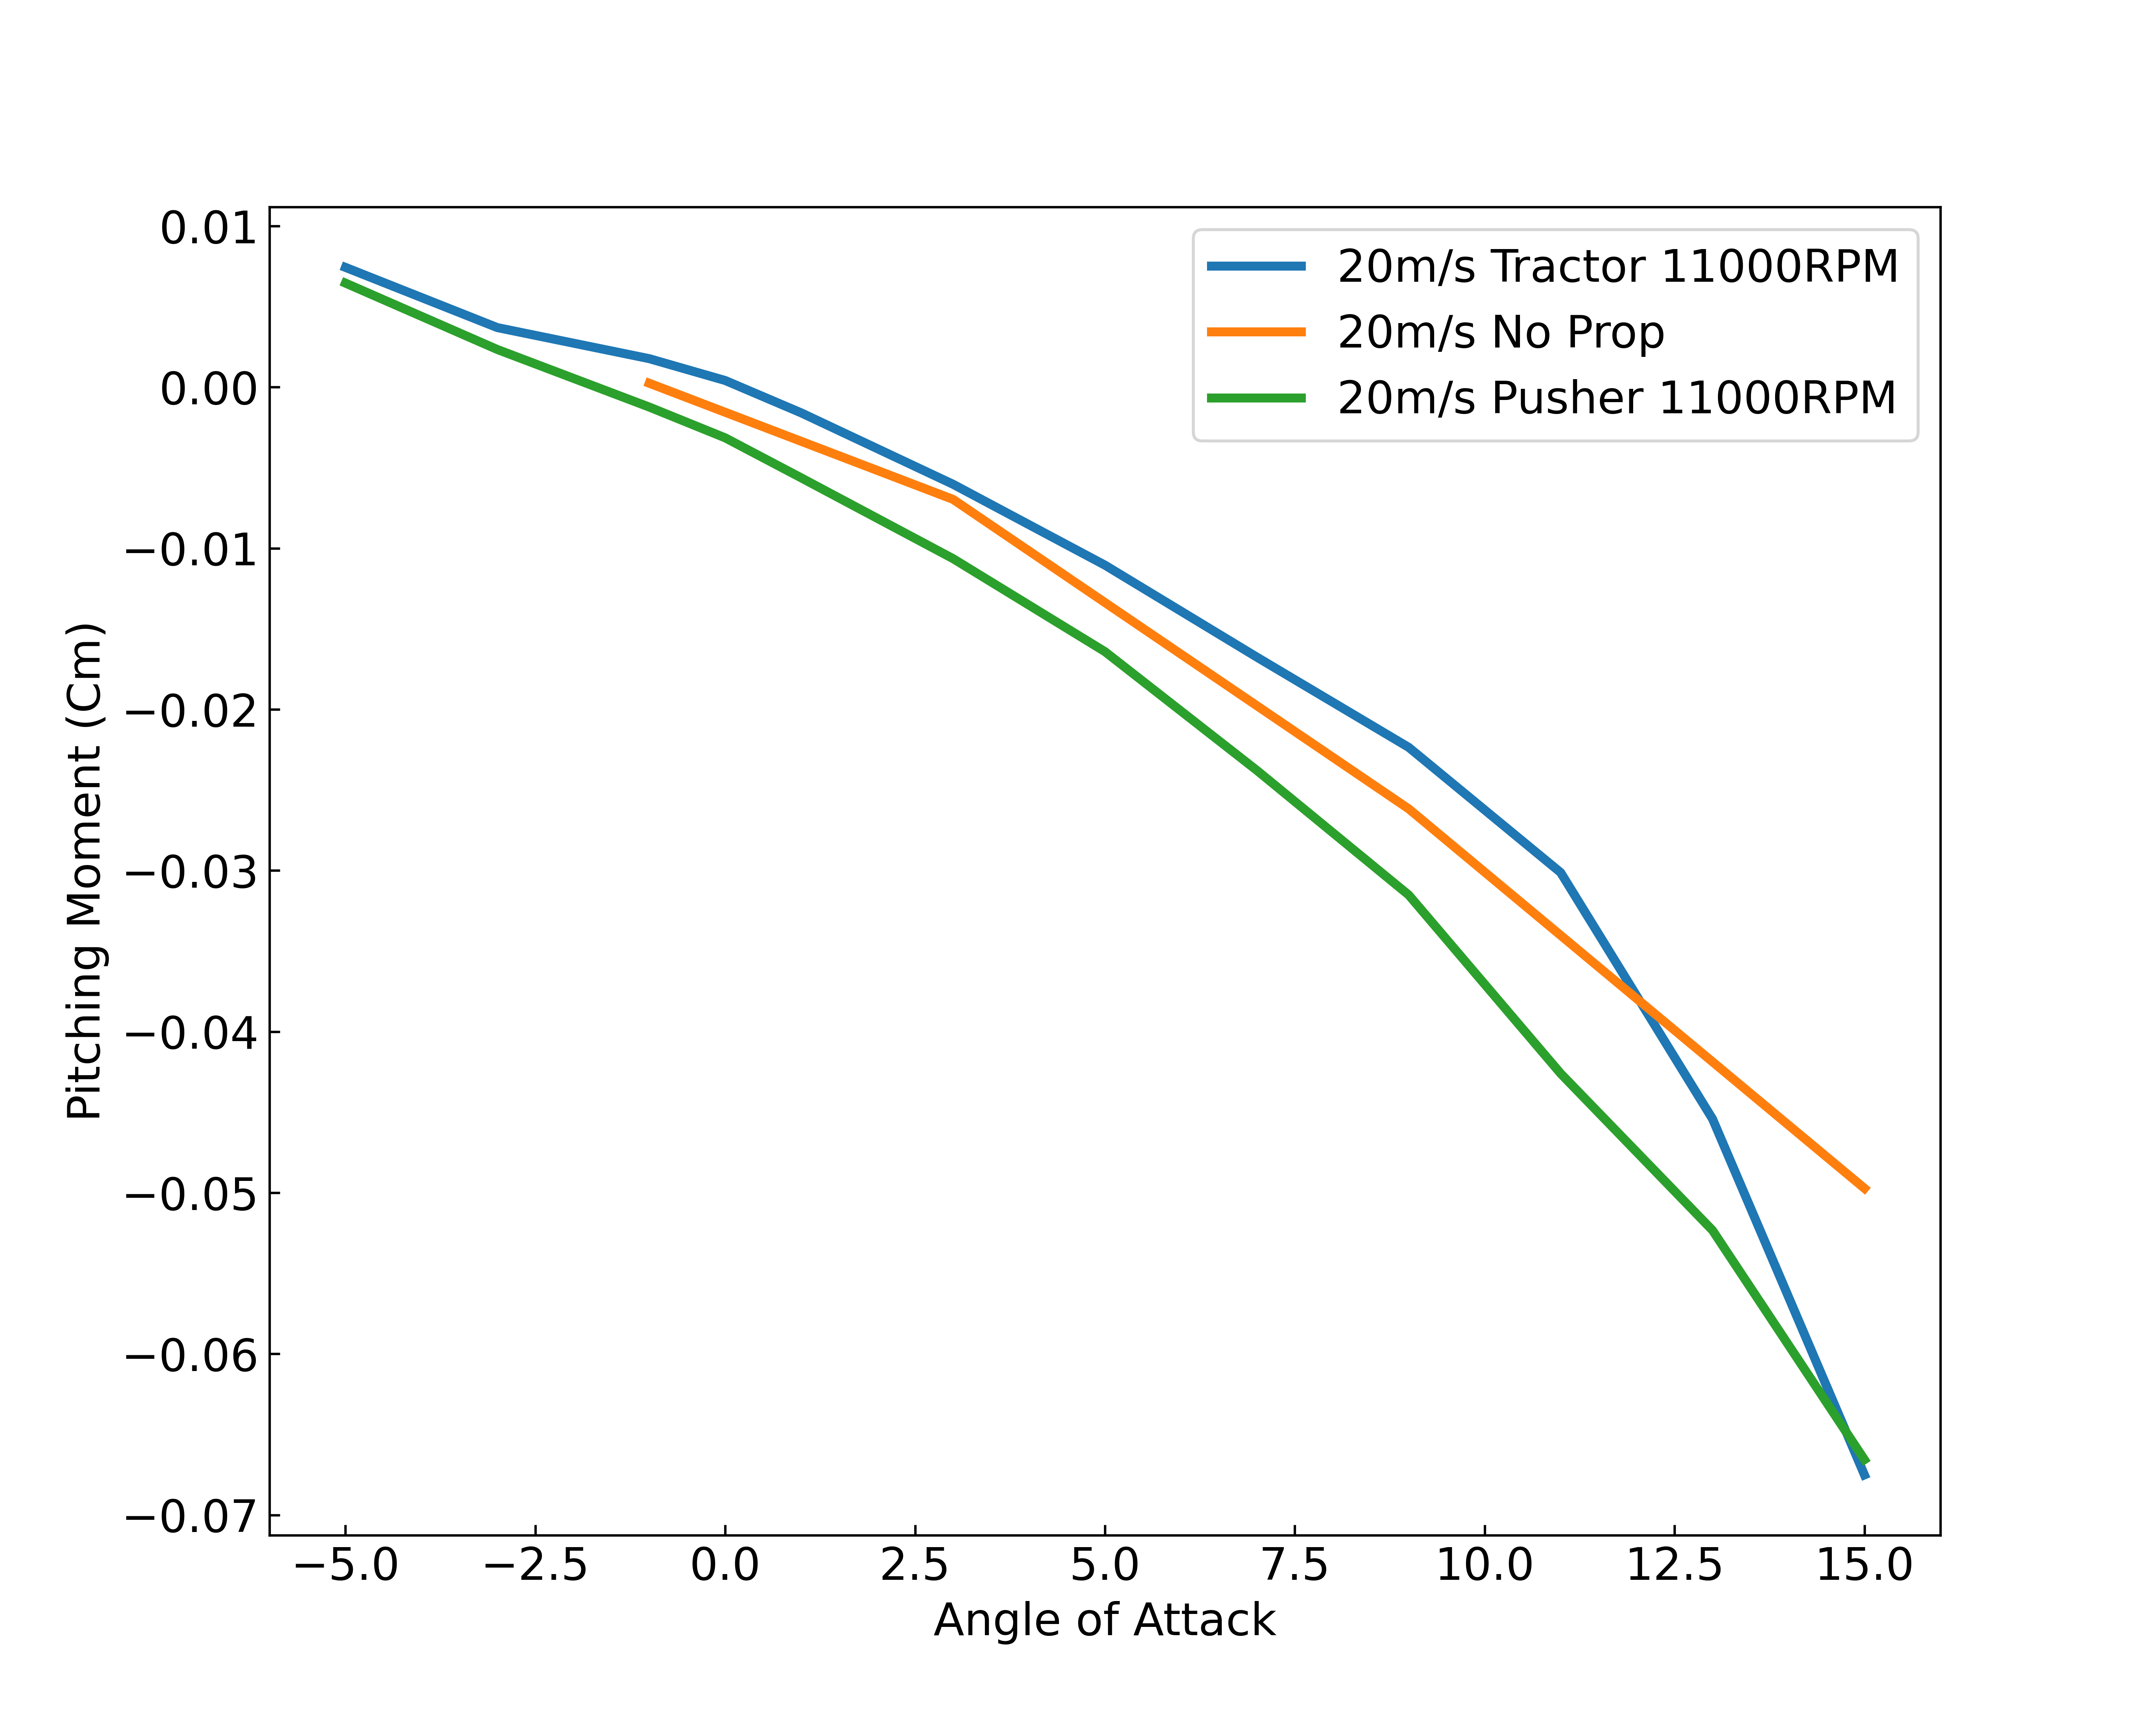
\includegraphics[width=\textwidth]{05_Results/Figs/Cm/20ms_11000RPM_Cm.png}
        \caption{Pitching Moment Coefficient at 20m/s airspeed and 11000RPM motor speed}
        \label{fig:Cm_20ms_11000}
    \end{subfigure}
    
\end{figure}

\subsection{Rolling Moment Coefficient}

The rolling coefficient for the tractor configuration when the propeller is run at 6000RPM was shifted downwards compared to both the pusher and no propeller configurations, leading to a decrease in the rolling moment for all speeds. When the propeller speed increased to 11000RPM, the tractor configuration did not show a significant shift downwards until a sharp drop, seen at $\approx$12.5$^{\circ}$ \acrshort{AoA}. However, the pusher configuration shows a shift upwards and an increase in the rolling coefficient for all airspeeds and propeller speeds. The rolling moment is largely due to the propeller torque effect in which an asymmetric roll is produced due to the propeller wing interaction, previously described in Section \ref{sec:propellerWingInteraction}. The tractor configuration also experiences a flow distribution change over the wings and fuselage due to the propeller's upwash and downwash effect, as described in Section \ref{sec:propellerWingInteraction}. These propeller effects affect the lift distribution across the wings' surface, shifting the roll moment coefficient upwards as one wing is in the upwash of the propeller blades and the other in the downwash airstream. As the angle of attack increases, this rolling moment increases until sharply dropping off in Figures \Cref{fig:Cl_roll_10ms_6000} to \Cref{fig:Cl_roll_20ms_11000} as the right wing of the MAV stalled first, creating a lift force imbalance as the left wing continues to produce a lift force. At the same time, the right-wing experiences flow separation due to stalling. The rolling moment Sharply raises as the left wing also stalls and the flow over the left wing separates. The pusher configuration shifts the rolling moment to a larger extent due to having a larger moment arm from the position of the propeller to the aerodynamic centre of the MAV model than the tractor configuration. The pusher configuration also shows a bump at 0$^{\circ}$ \acrshort{AoA} for all airspeeds, while the tractor configuration shows this only when the propeller is running at 11000RPM. The rolling moment also decreases after 2.5$^{\circ}$ \acrshort{AoA} for the tractor configuration when the propeller runs at 11000RPM. \todo{explaination??} The increases in roll moment at 0$^{\circ}$ \acrshort{AoA} is likely due to an interaction with the wing and/or the wings wake. However, more investigation needs to validate this.  

\begin{figure}[H]
    \centering
    \begin{subfigure}[b]{0.467\textwidth}
        \centering
        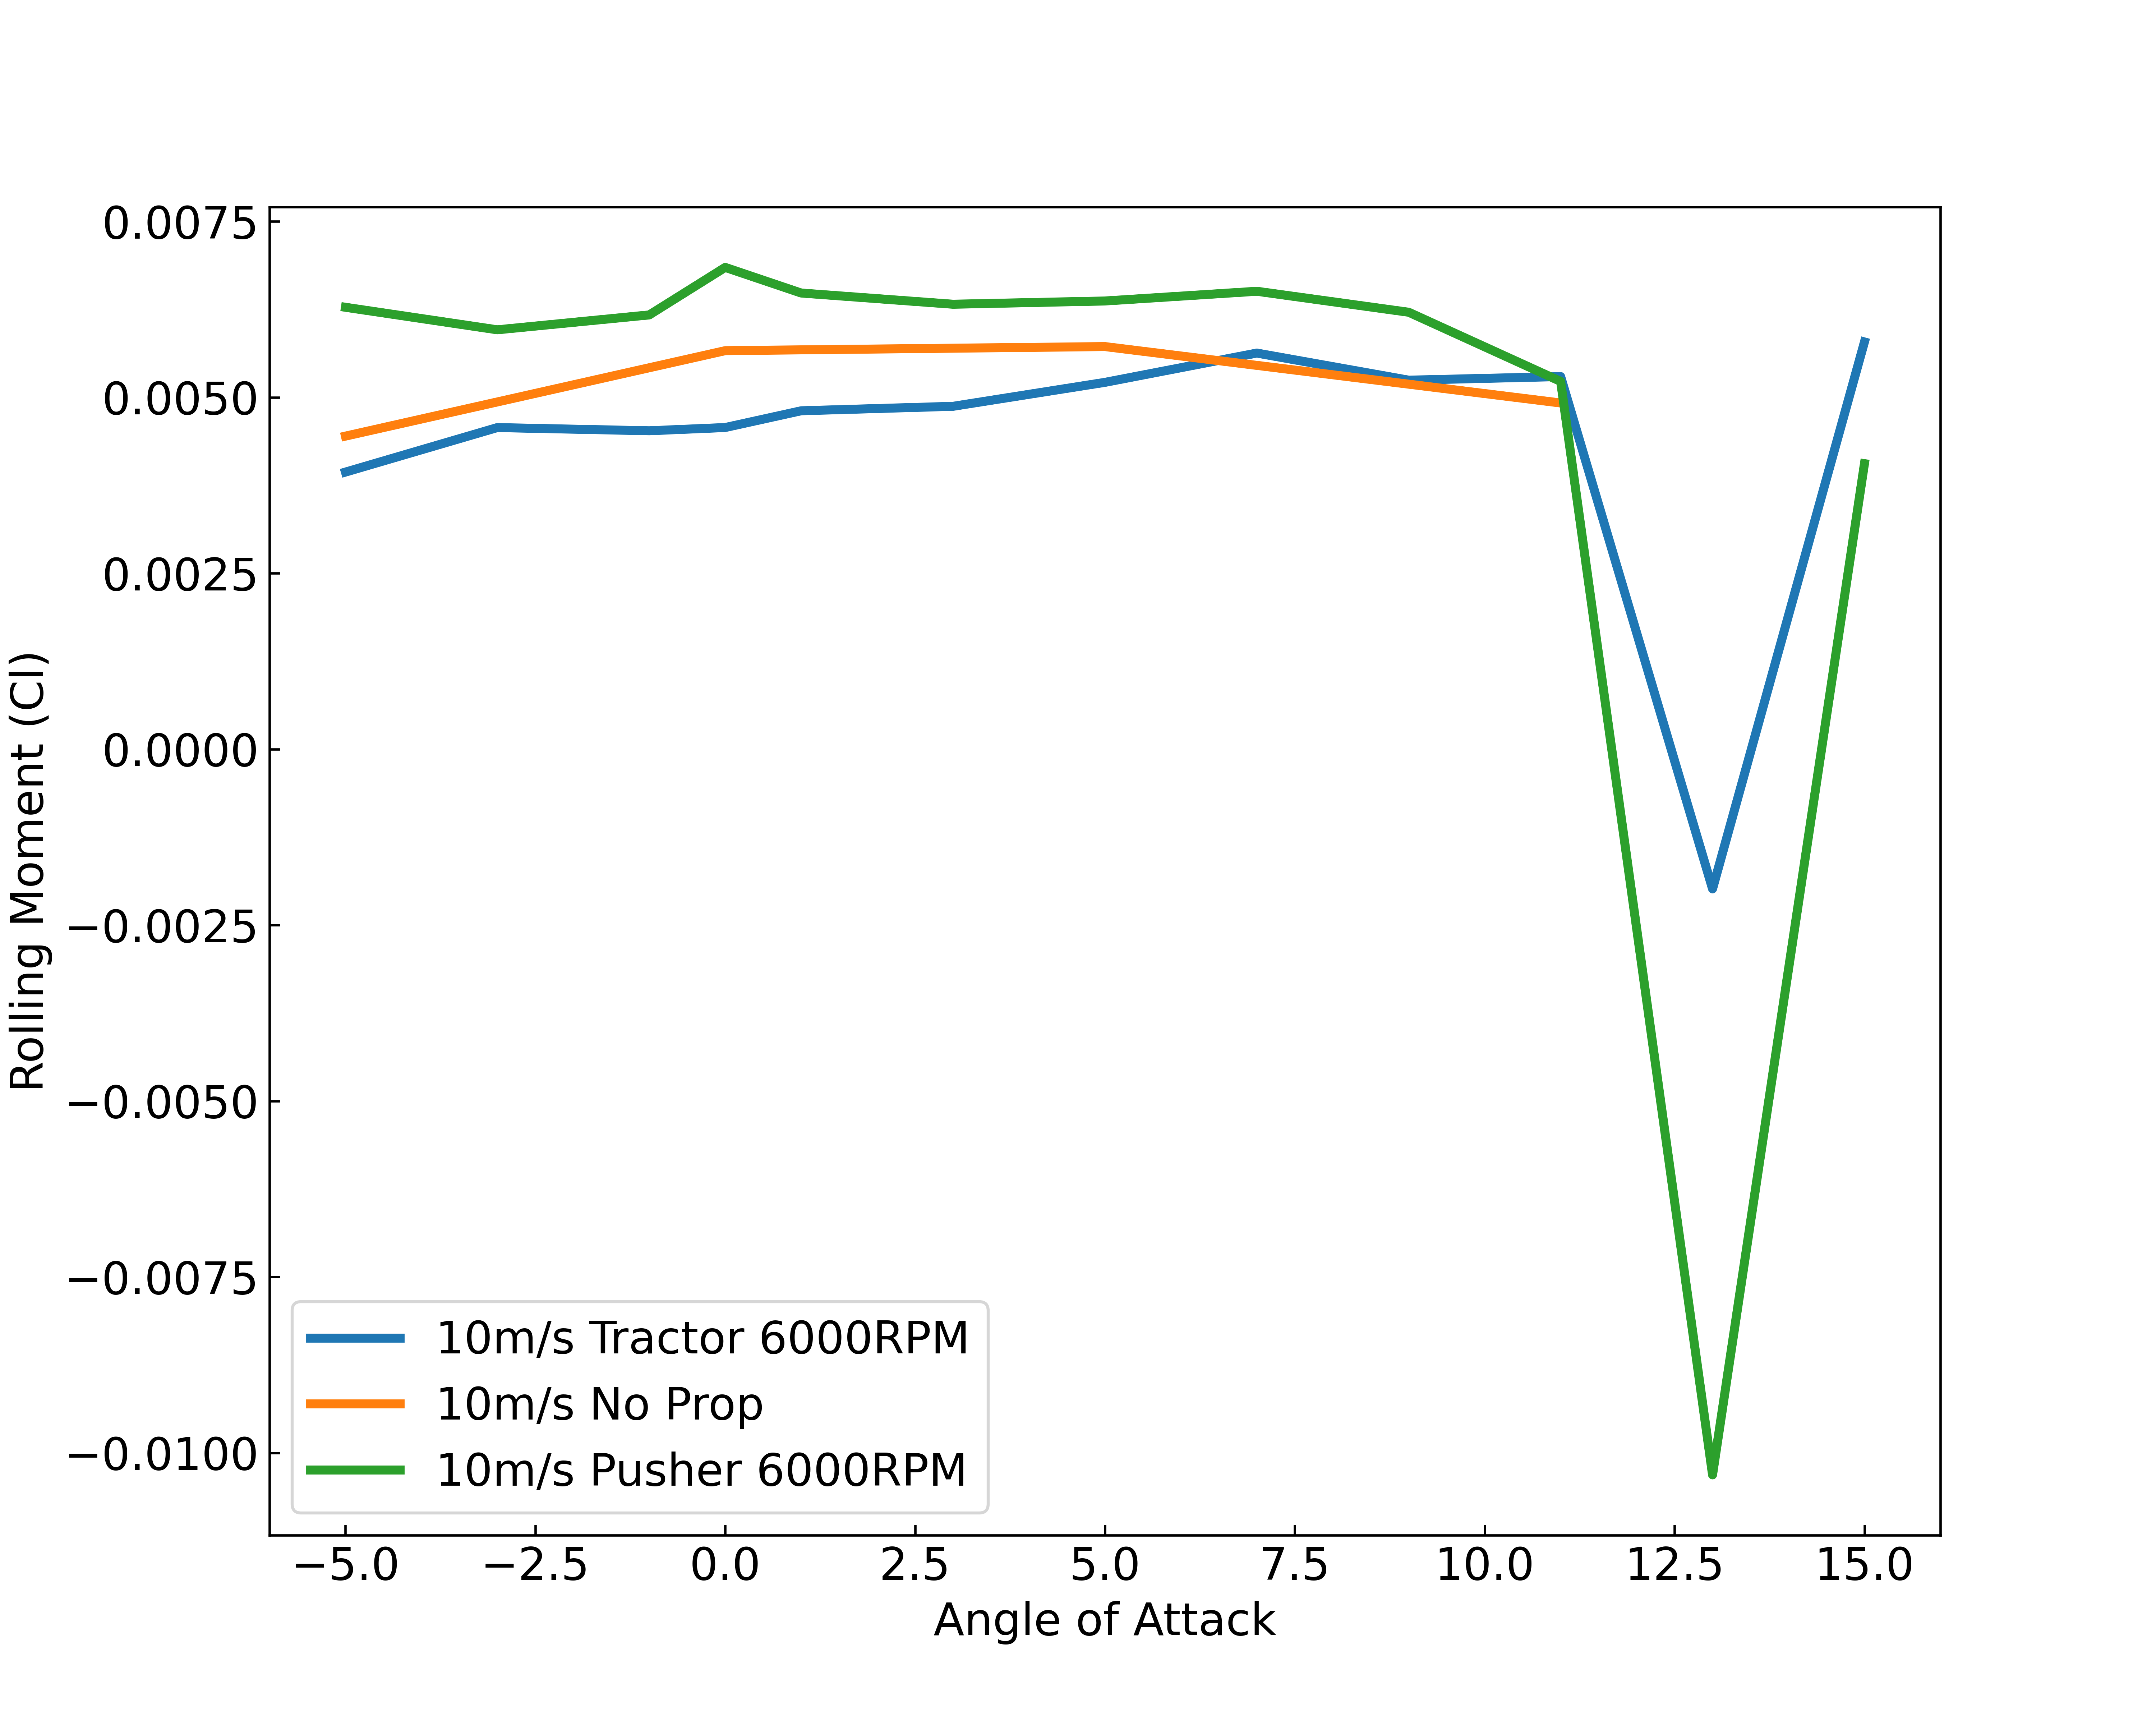
\includegraphics[width=\textwidth]{05_Results/Figs/Cl_roll/10ms_6000RPM_Cl_roll.png}
        \caption{Rolling Moment Coefficient at 10m/s airspeed and 6000RPM motor speed}
        \label{fig:Cl_roll_10ms_6000}
    \end{subfigure}
    \begin{subfigure}[b]{0.467\textwidth}
        \centering
        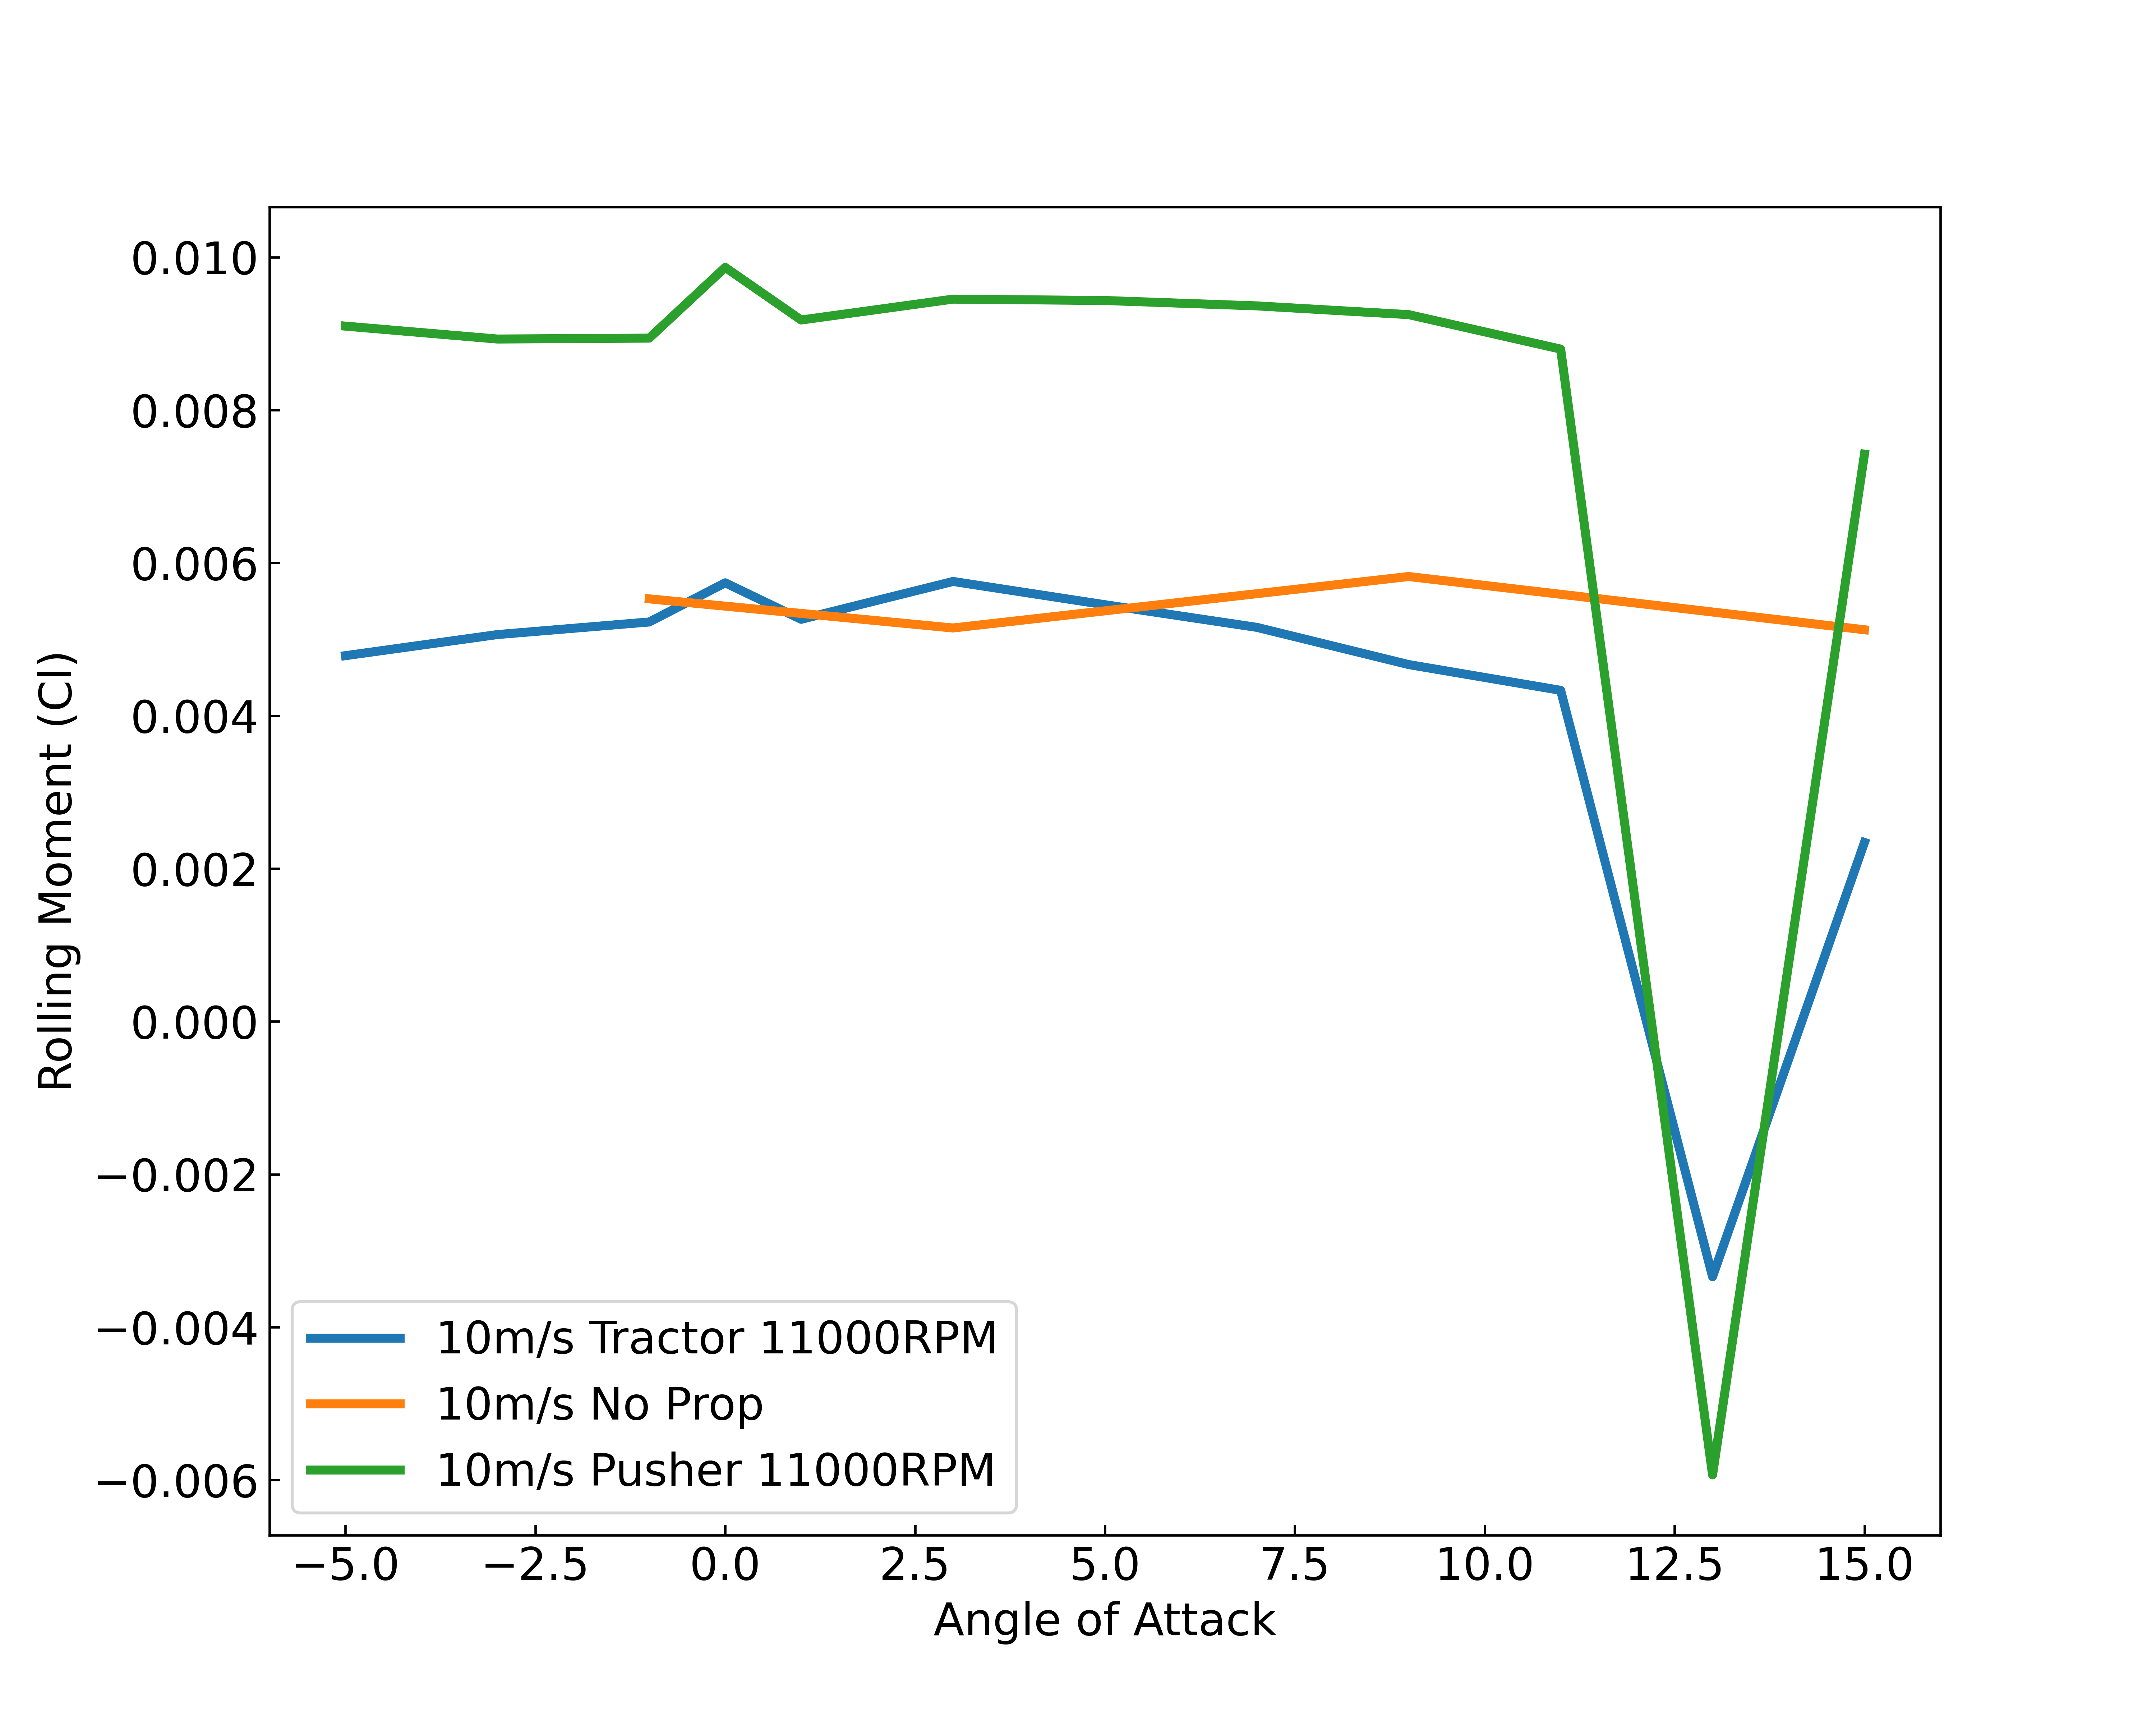
\includegraphics[width=\textwidth]{05_Results/Figs/Cl_roll/10ms_11000RPM_Cl.png}
        \caption{Rolling Moment Coefficient at 10m/s airspeed and 11000RPM motor speed}
        \label{fig:Cl_roll_10ms_11000}
    \end{subfigure}
    \begin{subfigure}[b]{0.467\textwidth}
        \centering
        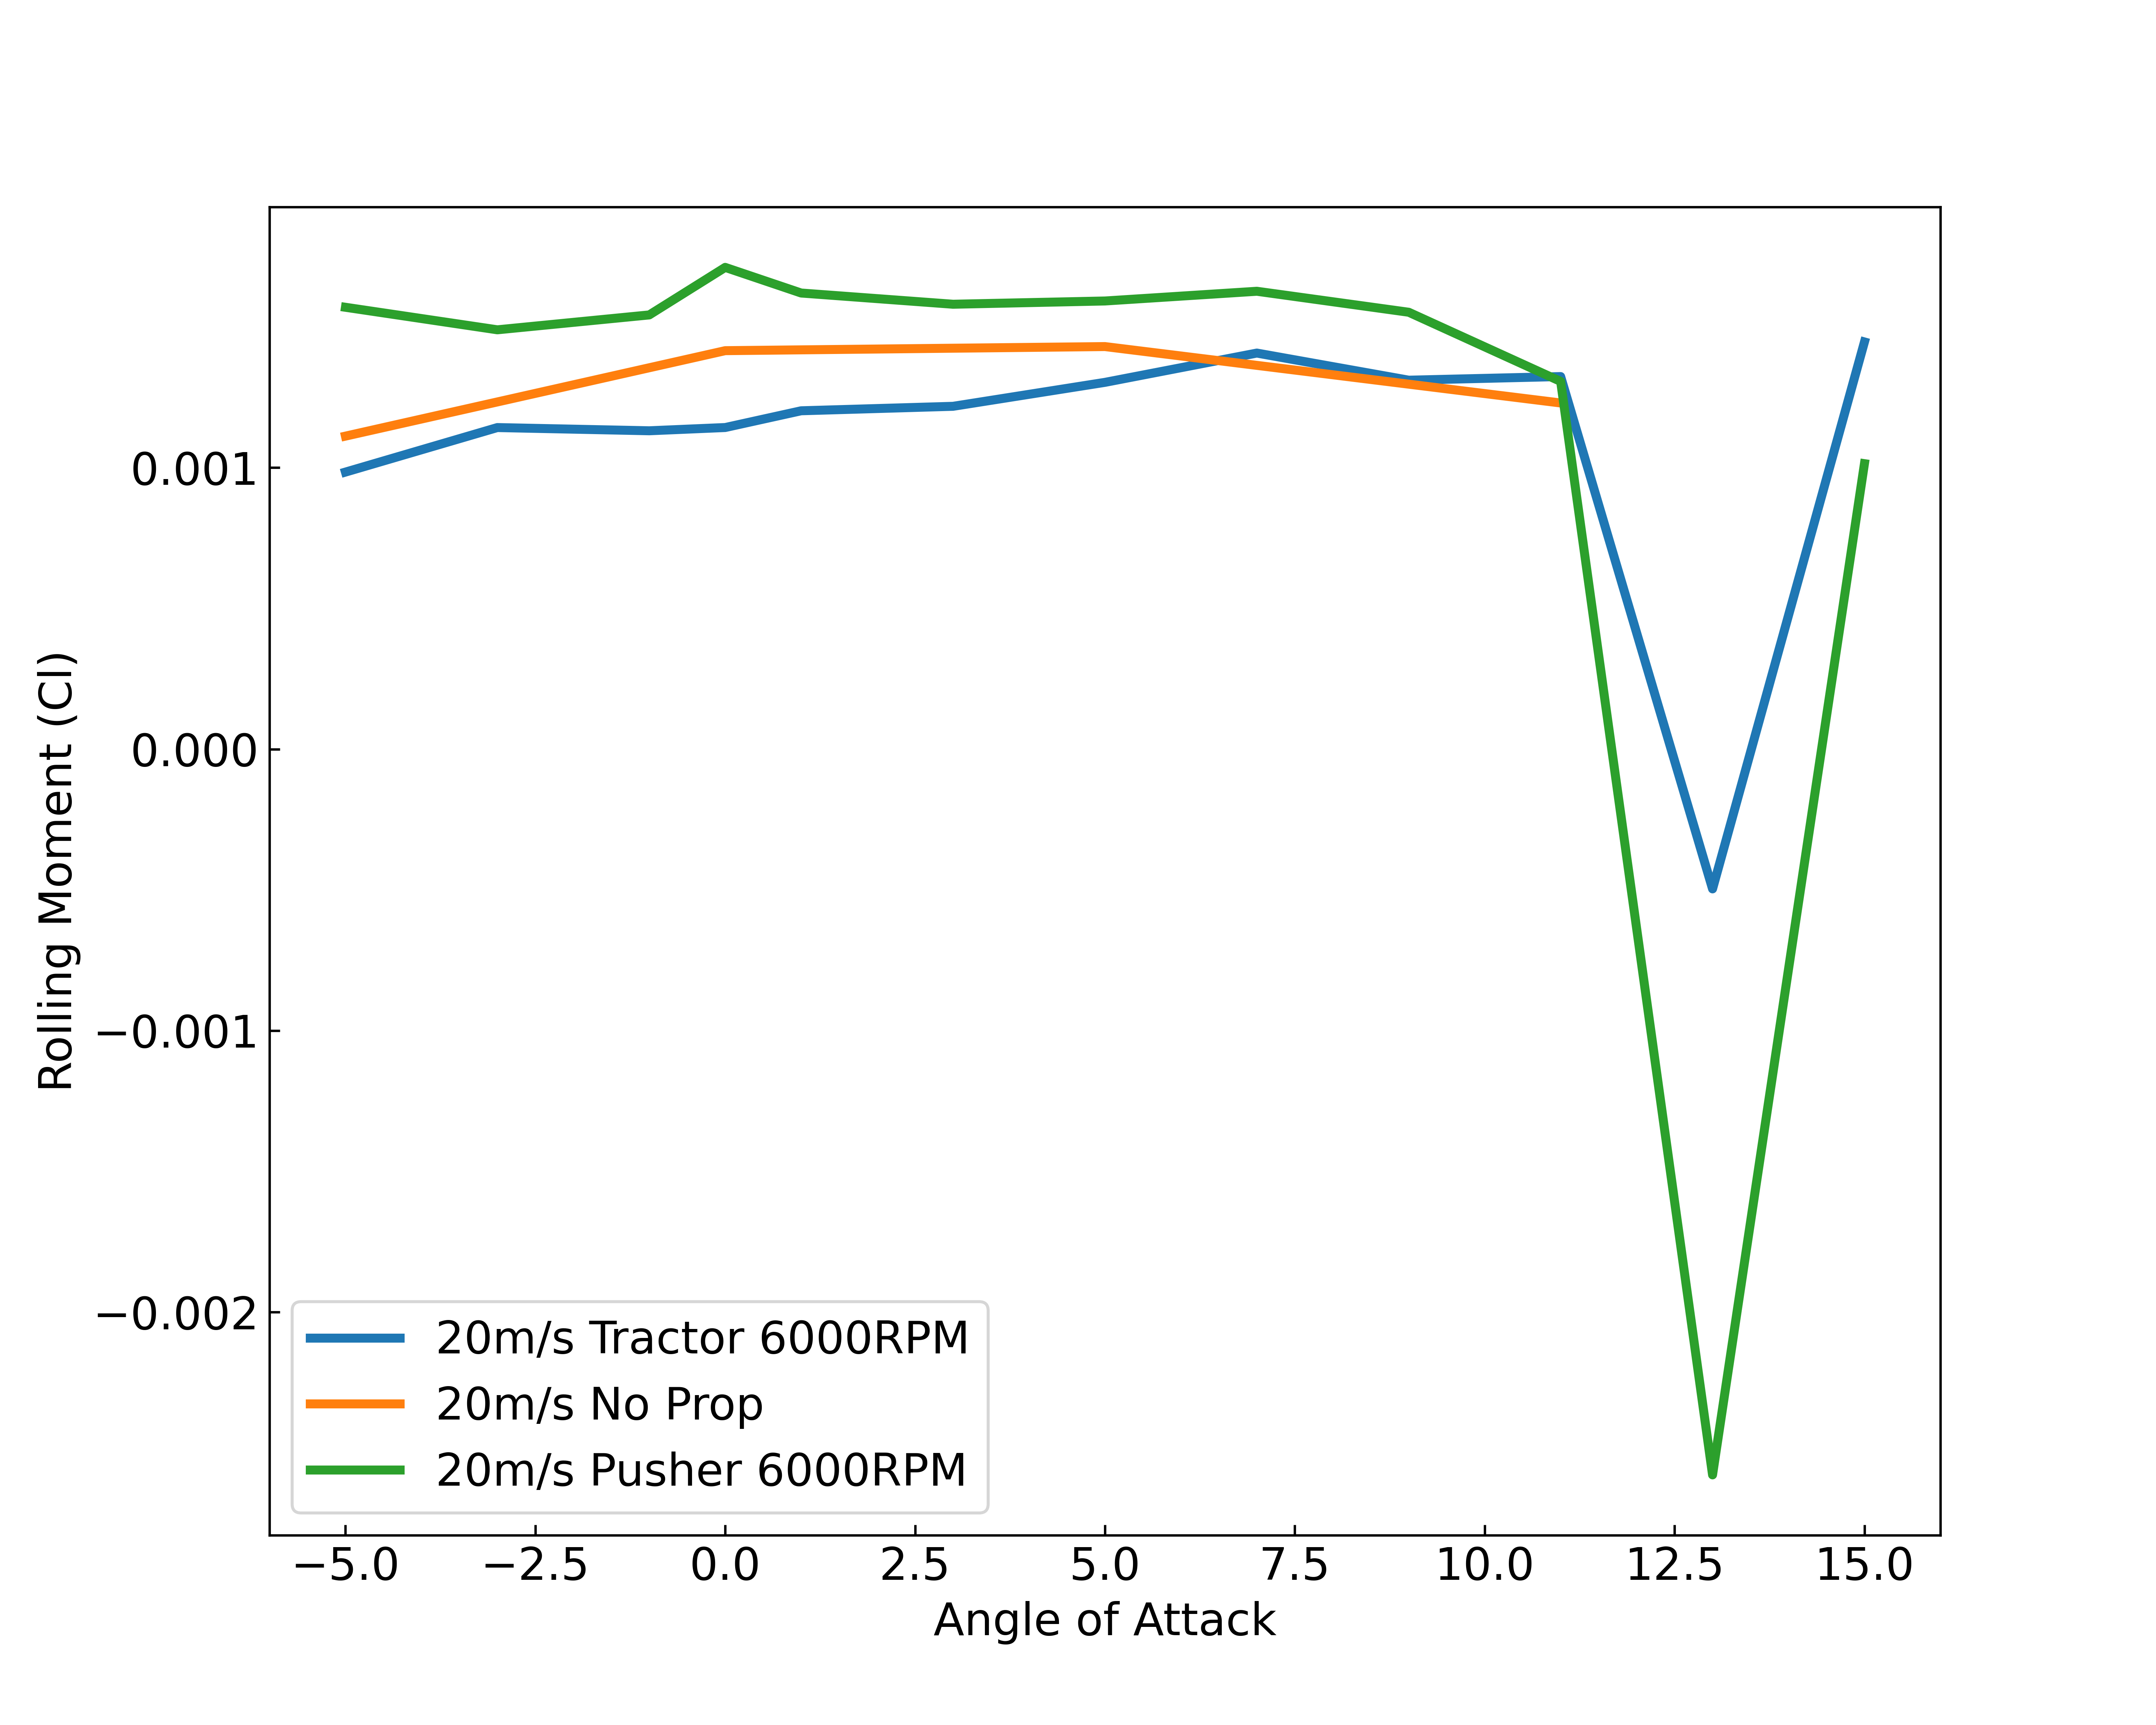
\includegraphics[width=\textwidth]{05_Results/Figs/Cl_roll/20ms_6000RPM_Cl_roll.png}
        \caption{Rolling Moment Coefficient at 20m/s airspeed and 6000RPM motor speed}
        \label{fig:Cl_roll_20ms_6000}
    \end{subfigure}
    \begin{subfigure}[b]{0.467\textwidth}
        \centering
        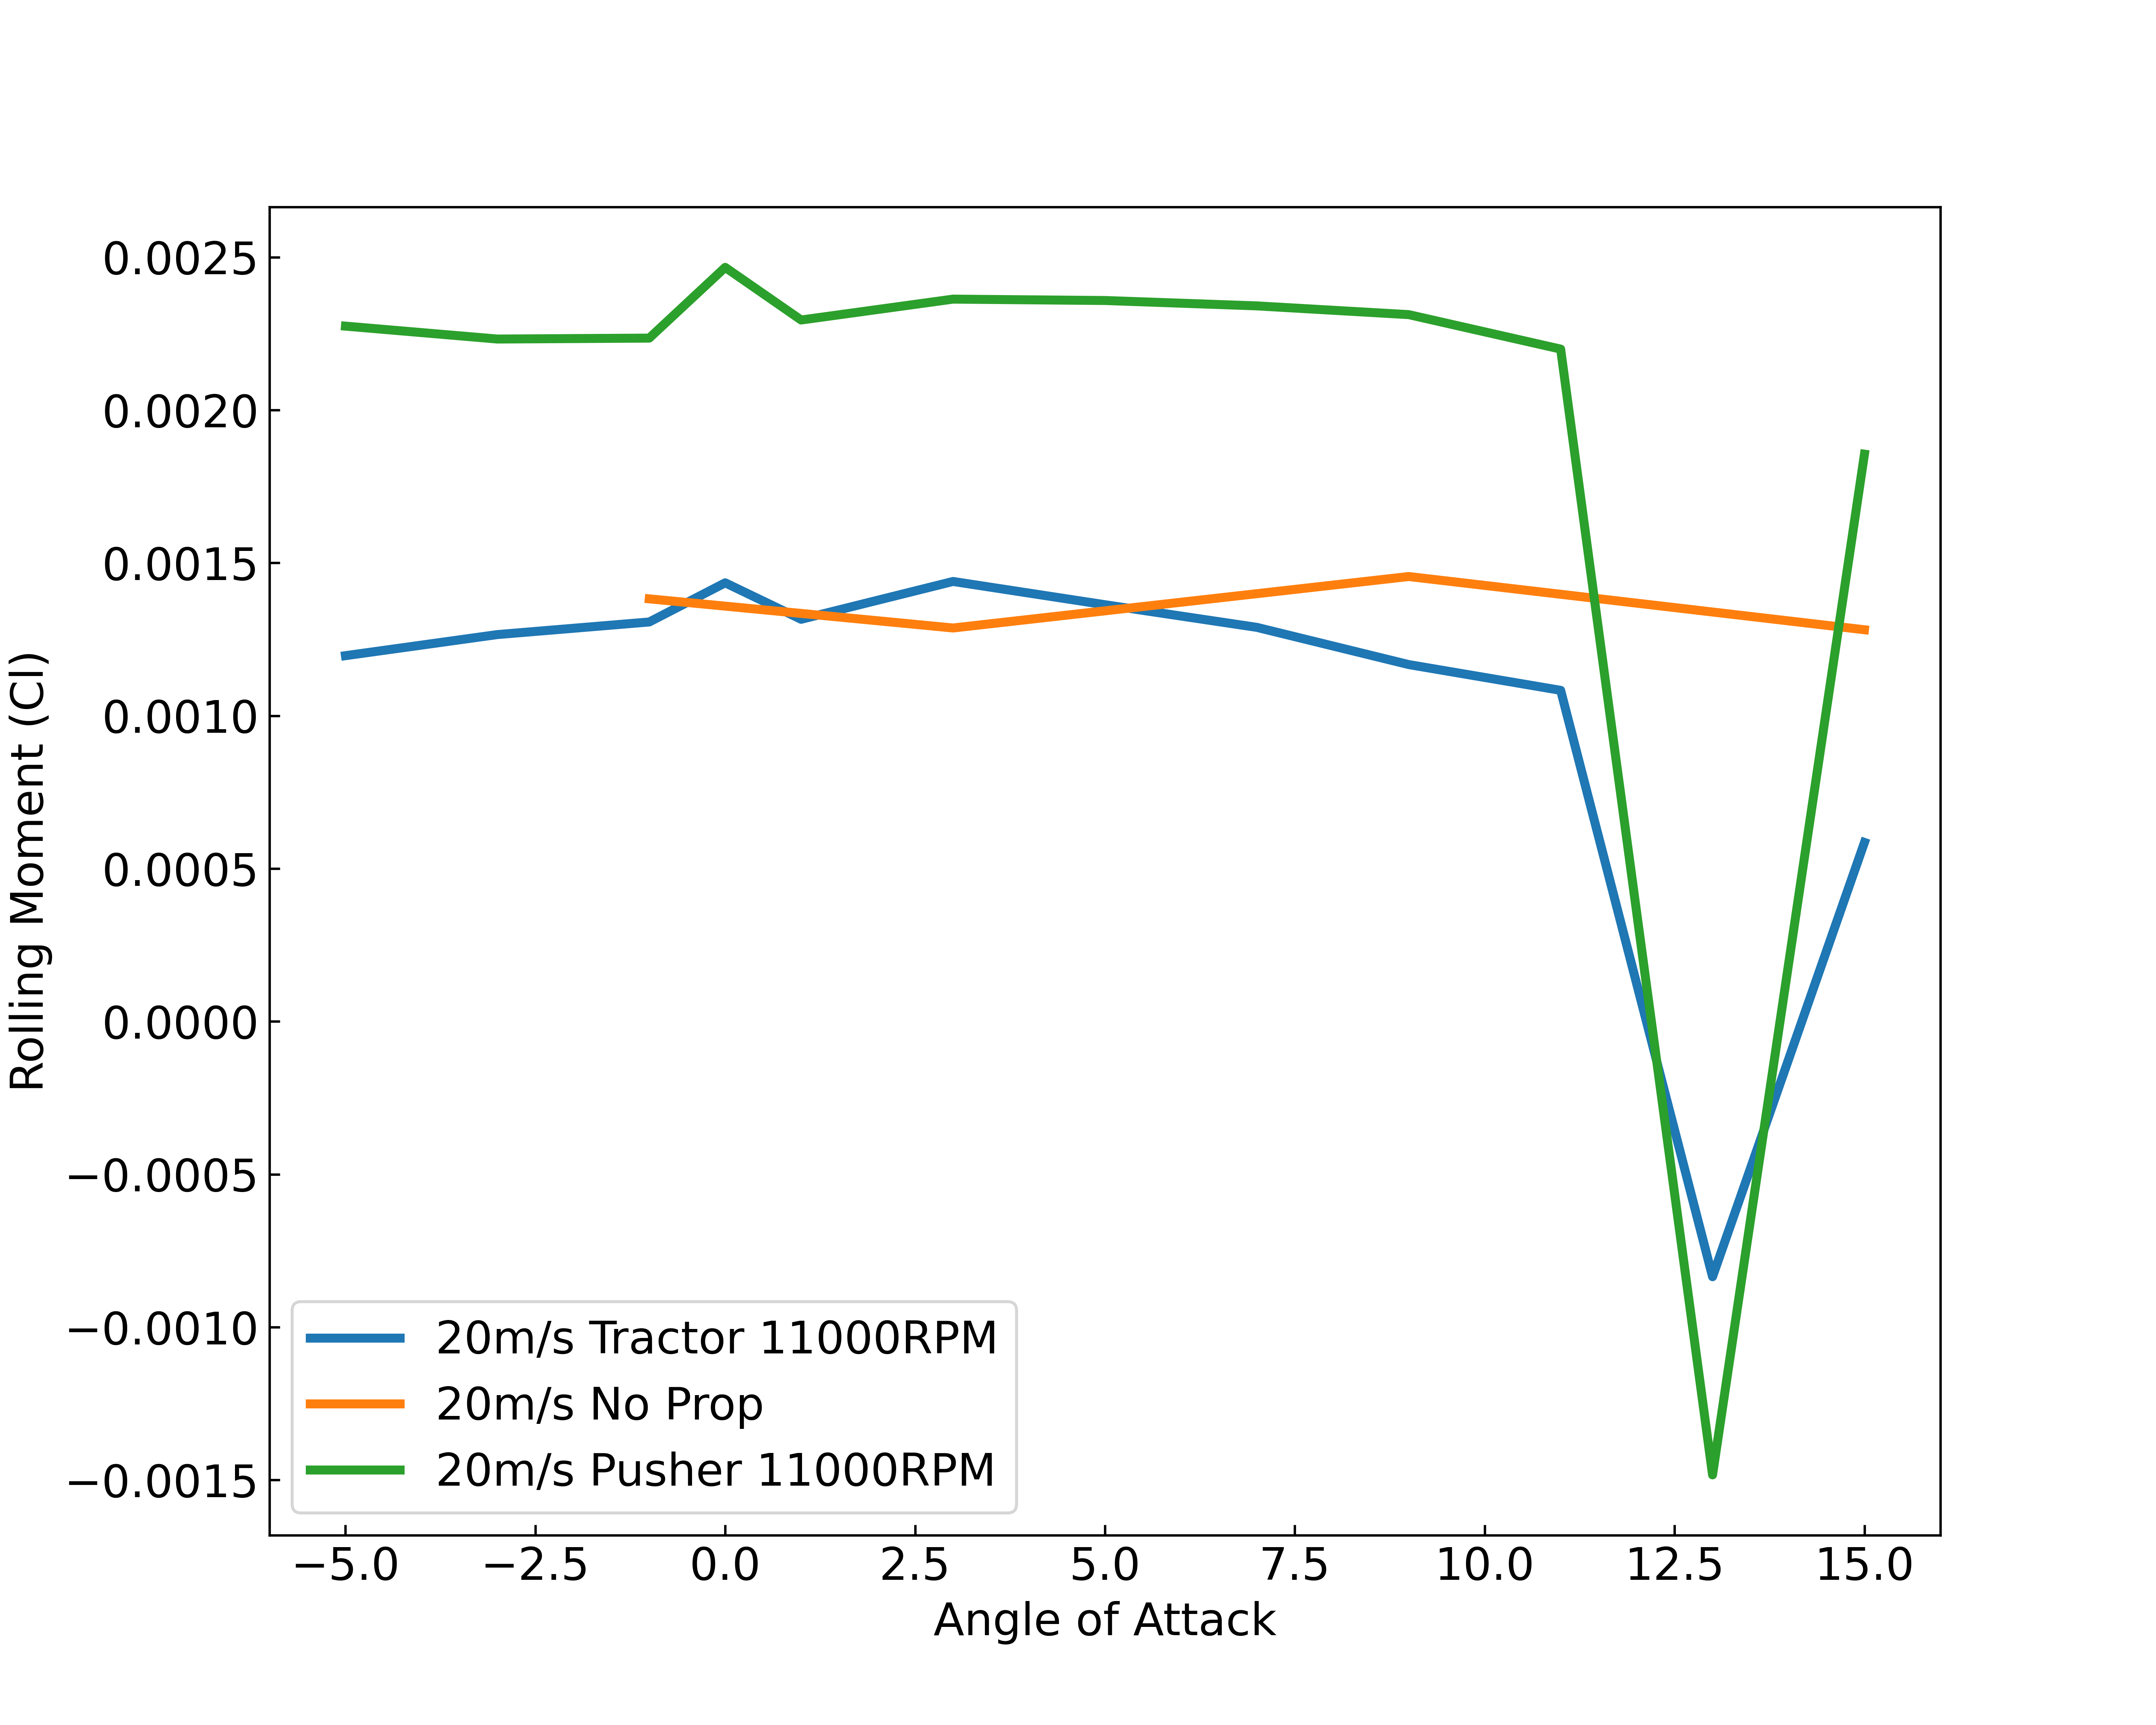
\includegraphics[width=\textwidth]{05_Results/Figs/Cl_roll/20ms_11000RPM_Cl.png}
        \caption{Rolling Moment Coefficient at 20m/s airspeed and 11000RPM motor speed}
        \label{fig:Cl_roll_20ms_11000}
    \end{subfigure}
\end{figure}


\subsection{Yawing Moment Coefficient}
 The yawing coefficient for the tractor configuration was shifted upwards compared to both the pusher and no propeller configurations. The yawing moment is also produced as a consequence of the roll moment produced. The aircraft roll moment remains relatively constant until the stall of the right wing at $\approx$12.5$^{\circ}$ \acrshort{AoA}. Hence the increase in the yawing moment as the aircraft \acrshort{AoA} increases is likely due to the effects of the roll being magnified as flow separation occurs. The roll moment causes an adverse yaw effect where the MAV naturally tends to yaw in the opposite direction of the roll \todo{cite}. This is due to the different lift and drag acting on each wing. As the angle of attack increases, the difference between the two wings in lift and drag increases, leading to an increase in the yaw moment for all configurations, airspeeds and propeller speeds except for the no propeller configuration when run at 20m$s^{-1}$. As the angle of attack increases, the yaw moment increases until sharply dropping off in Figures \Cref{fig:Cl_roll_10ms_6000} to \Cref{fig:Cl_roll_20ms_11000}. This is also due to the stall of the right-wing, creating a lift force imbalance as the left wing continues to produce a lift force while the right-wing experiences flow separation due to the increase in \acrshort{AoA}. The yawing moment also sharply raises as the flow over the left wing also separates and stalls beyond $\approx$12.5$^{\circ}$ \acrshort{AoA}. Several kinks are seen in Figures \Cref{fig:Cl_roll_10ms_6000} to \Cref{fig:Cl_roll_20ms_11000}, the most notable being the changes in gradient seen for the pusher configuration with a propeller speed of 6000RPM in Figures \Cref{fig:Cl_roll_10ms_6000} and \Cref{fig:Cl_roll_20ms_6000} at $\approx$0$^{\circ}$, $\approx$2.5$^{\circ}$ and $\approx$7.5$^{\circ}$\acrshort{AoA}. These changes can be partially attributed to the roll moment changes seen in Figures 
 \Cref{fig:Cl_roll_10ms_6000} to \Cref{fig:Cl_roll_20ms_11000}, which creates an adverse yaw effect that acts opposite to the roll. 

\begin{figure}[H]
    \centering
    \begin{subfigure}[b]{0.467\textwidth}
        \centering
        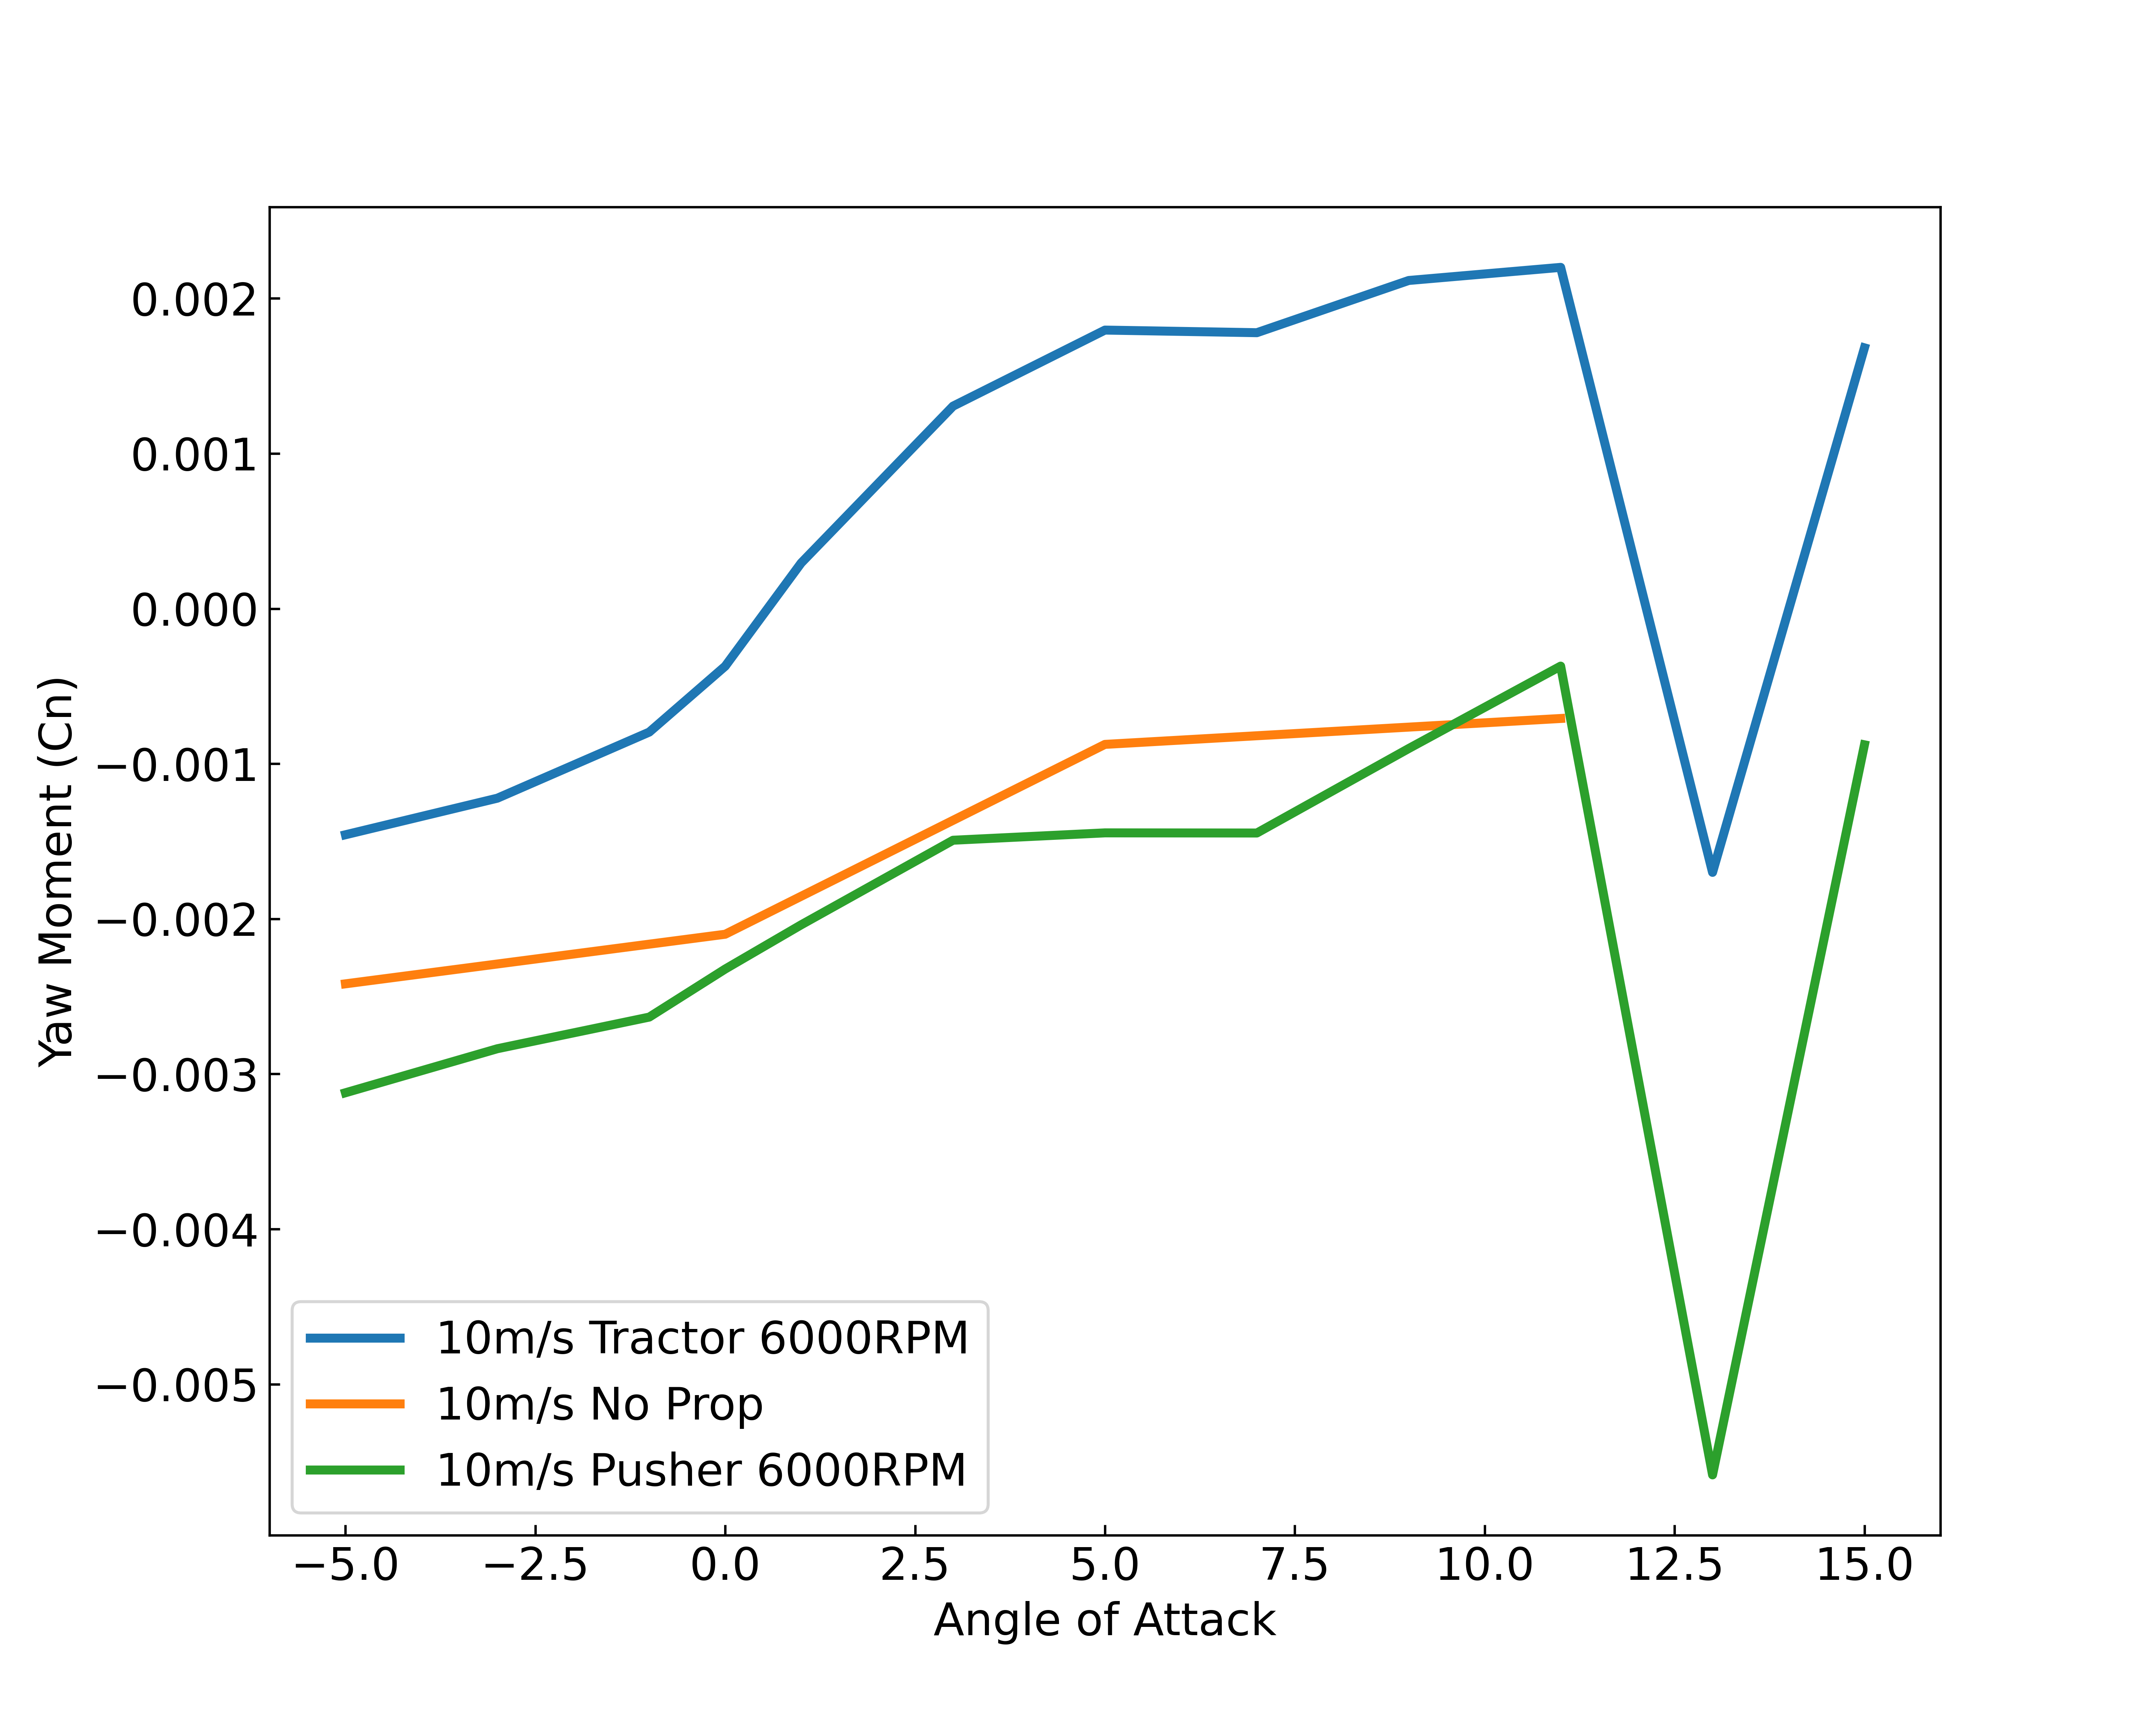
\includegraphics[width=\textwidth]{05_Results/Figs/Cn/10ms_6000RPM_Cn.png}
        \caption{Yawing Moment Coefficient at 10m/s airspeed and 6000RPM motor speed}
        \label{fig:Cn_10ms_6000}
    \end{subfigure}
    \begin{subfigure}[b]{0.467\textwidth}
        \centering
        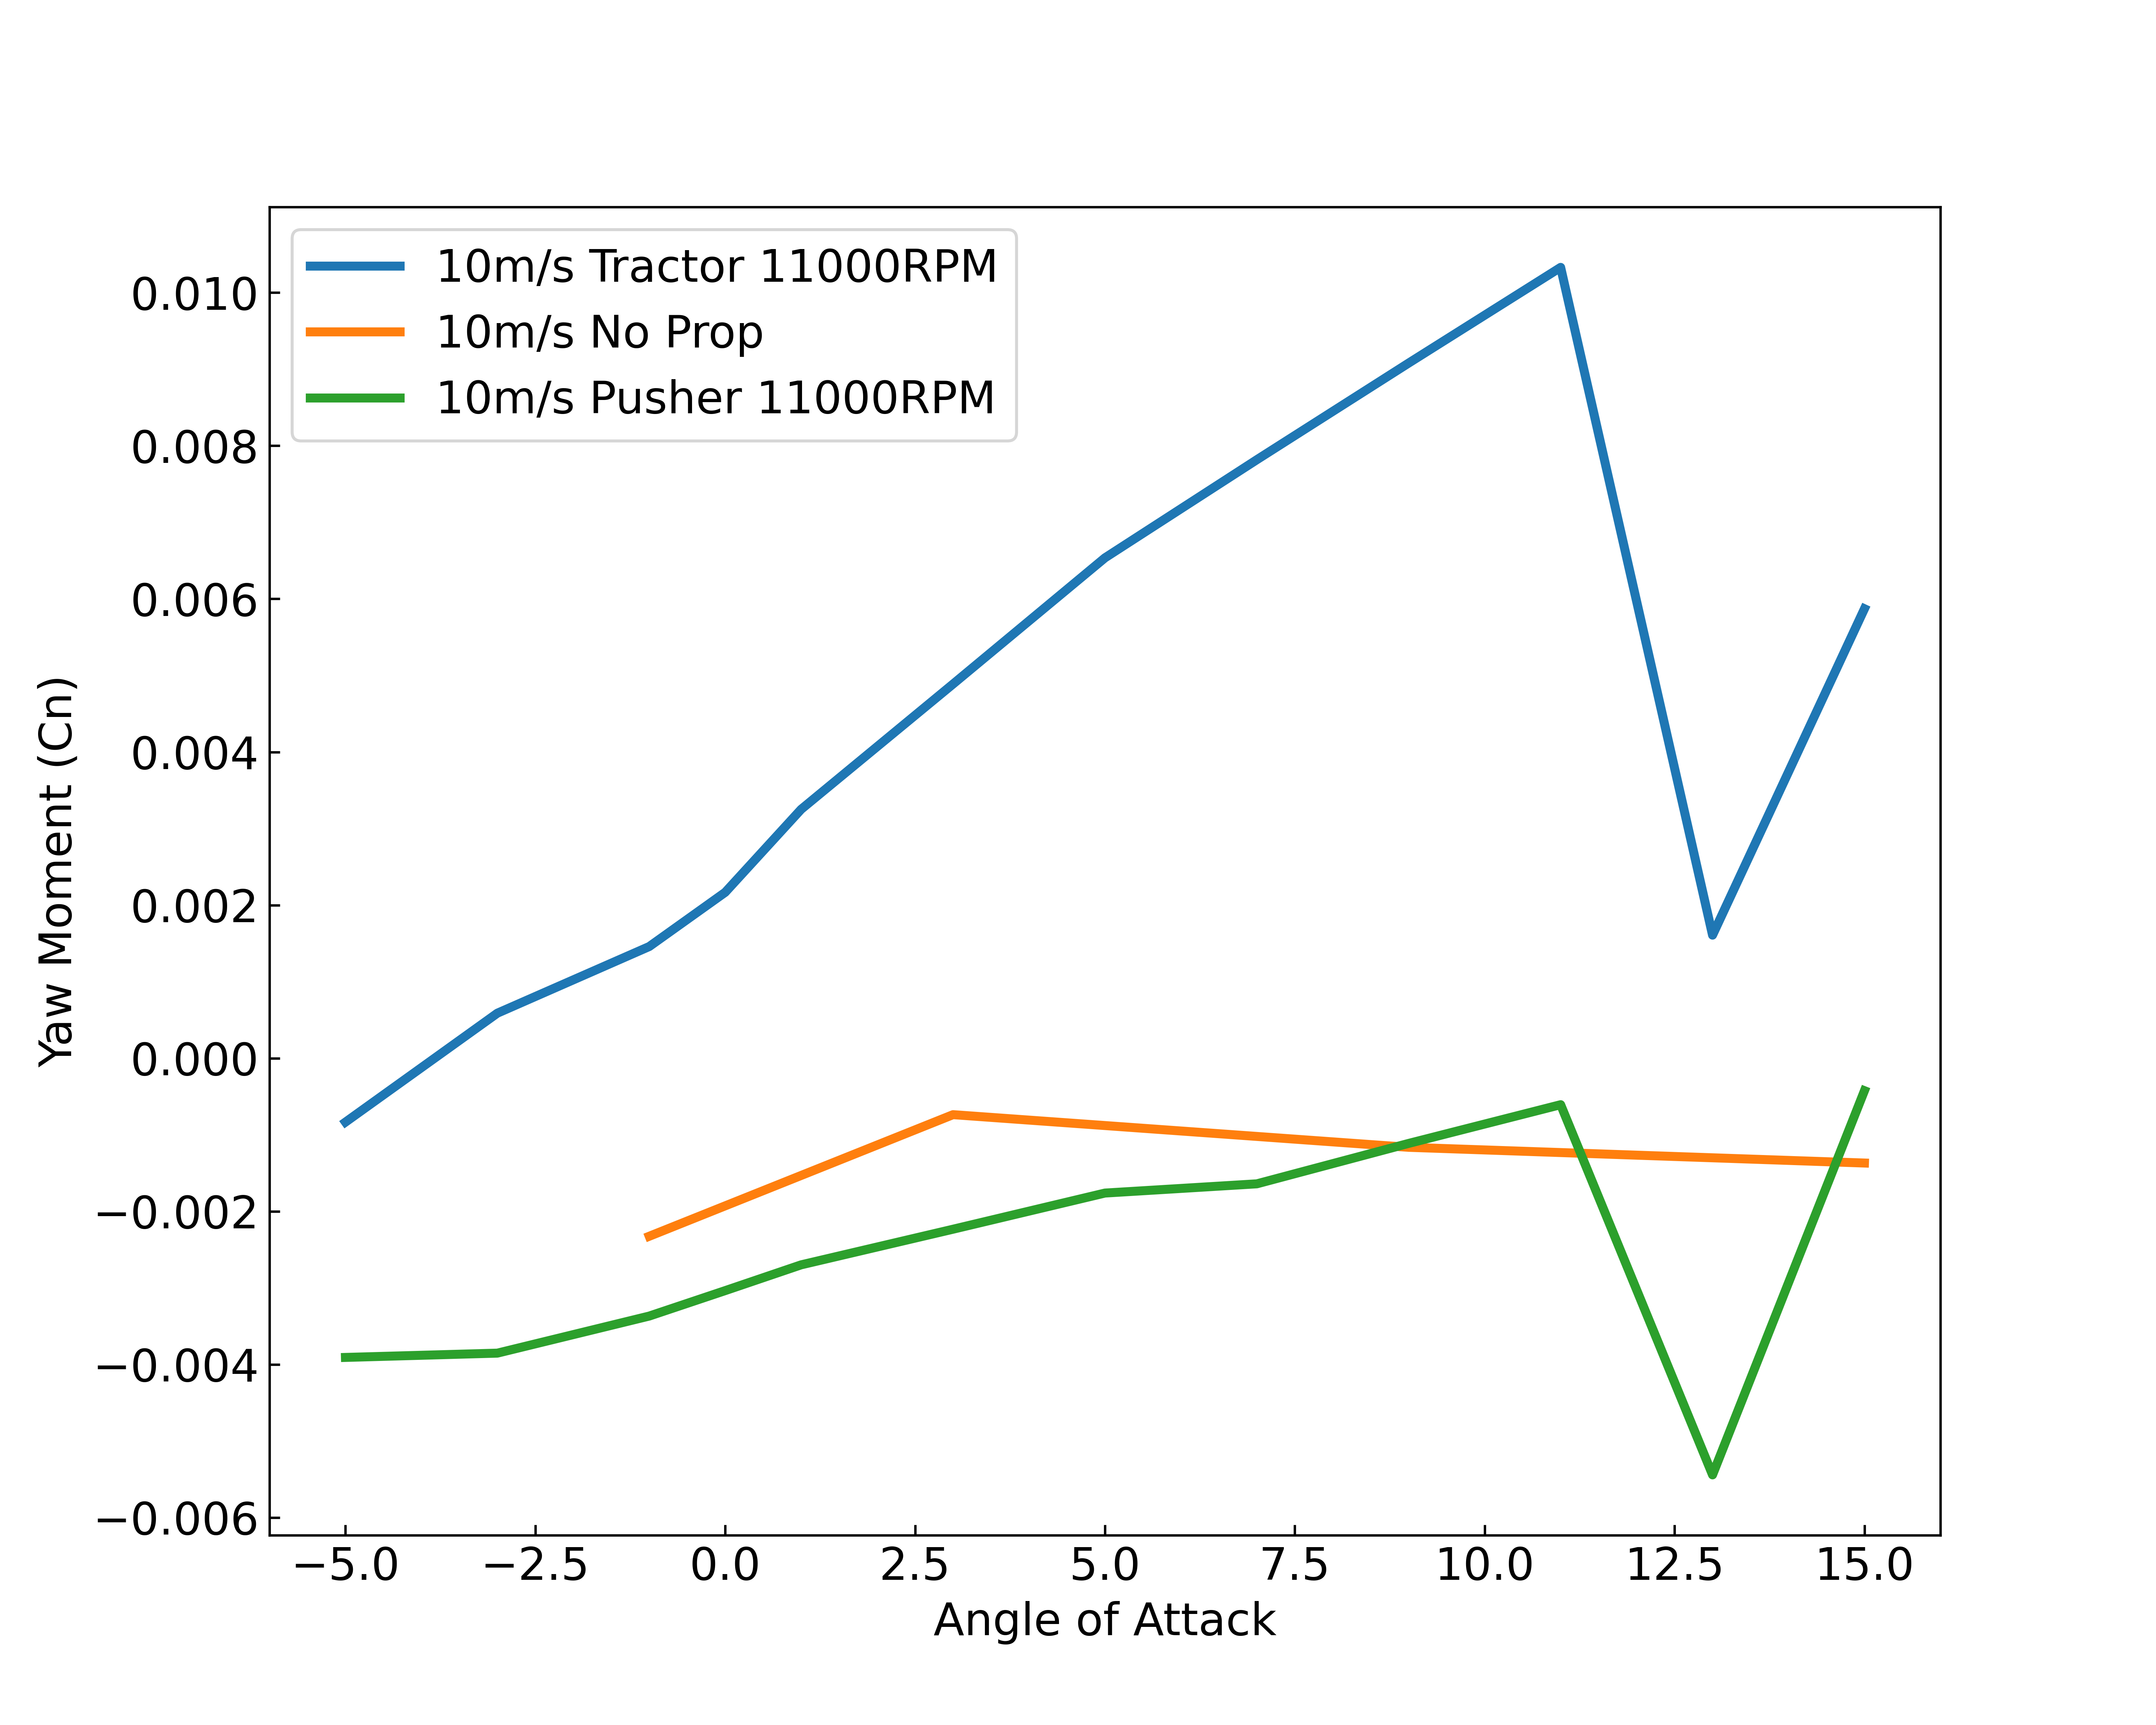
\includegraphics[width=\textwidth]{05_Results/Figs/Cn/10ms_11000RPM_Cn.png}
        \caption{Yawing Moment Coefficient at 10m/s airspeed and 11000RPM motor speed}
        \label{fig:Cn_10ms_11000}
    \end{subfigure}
    \begin{subfigure}[b]{0.467\textwidth}
        \centering
        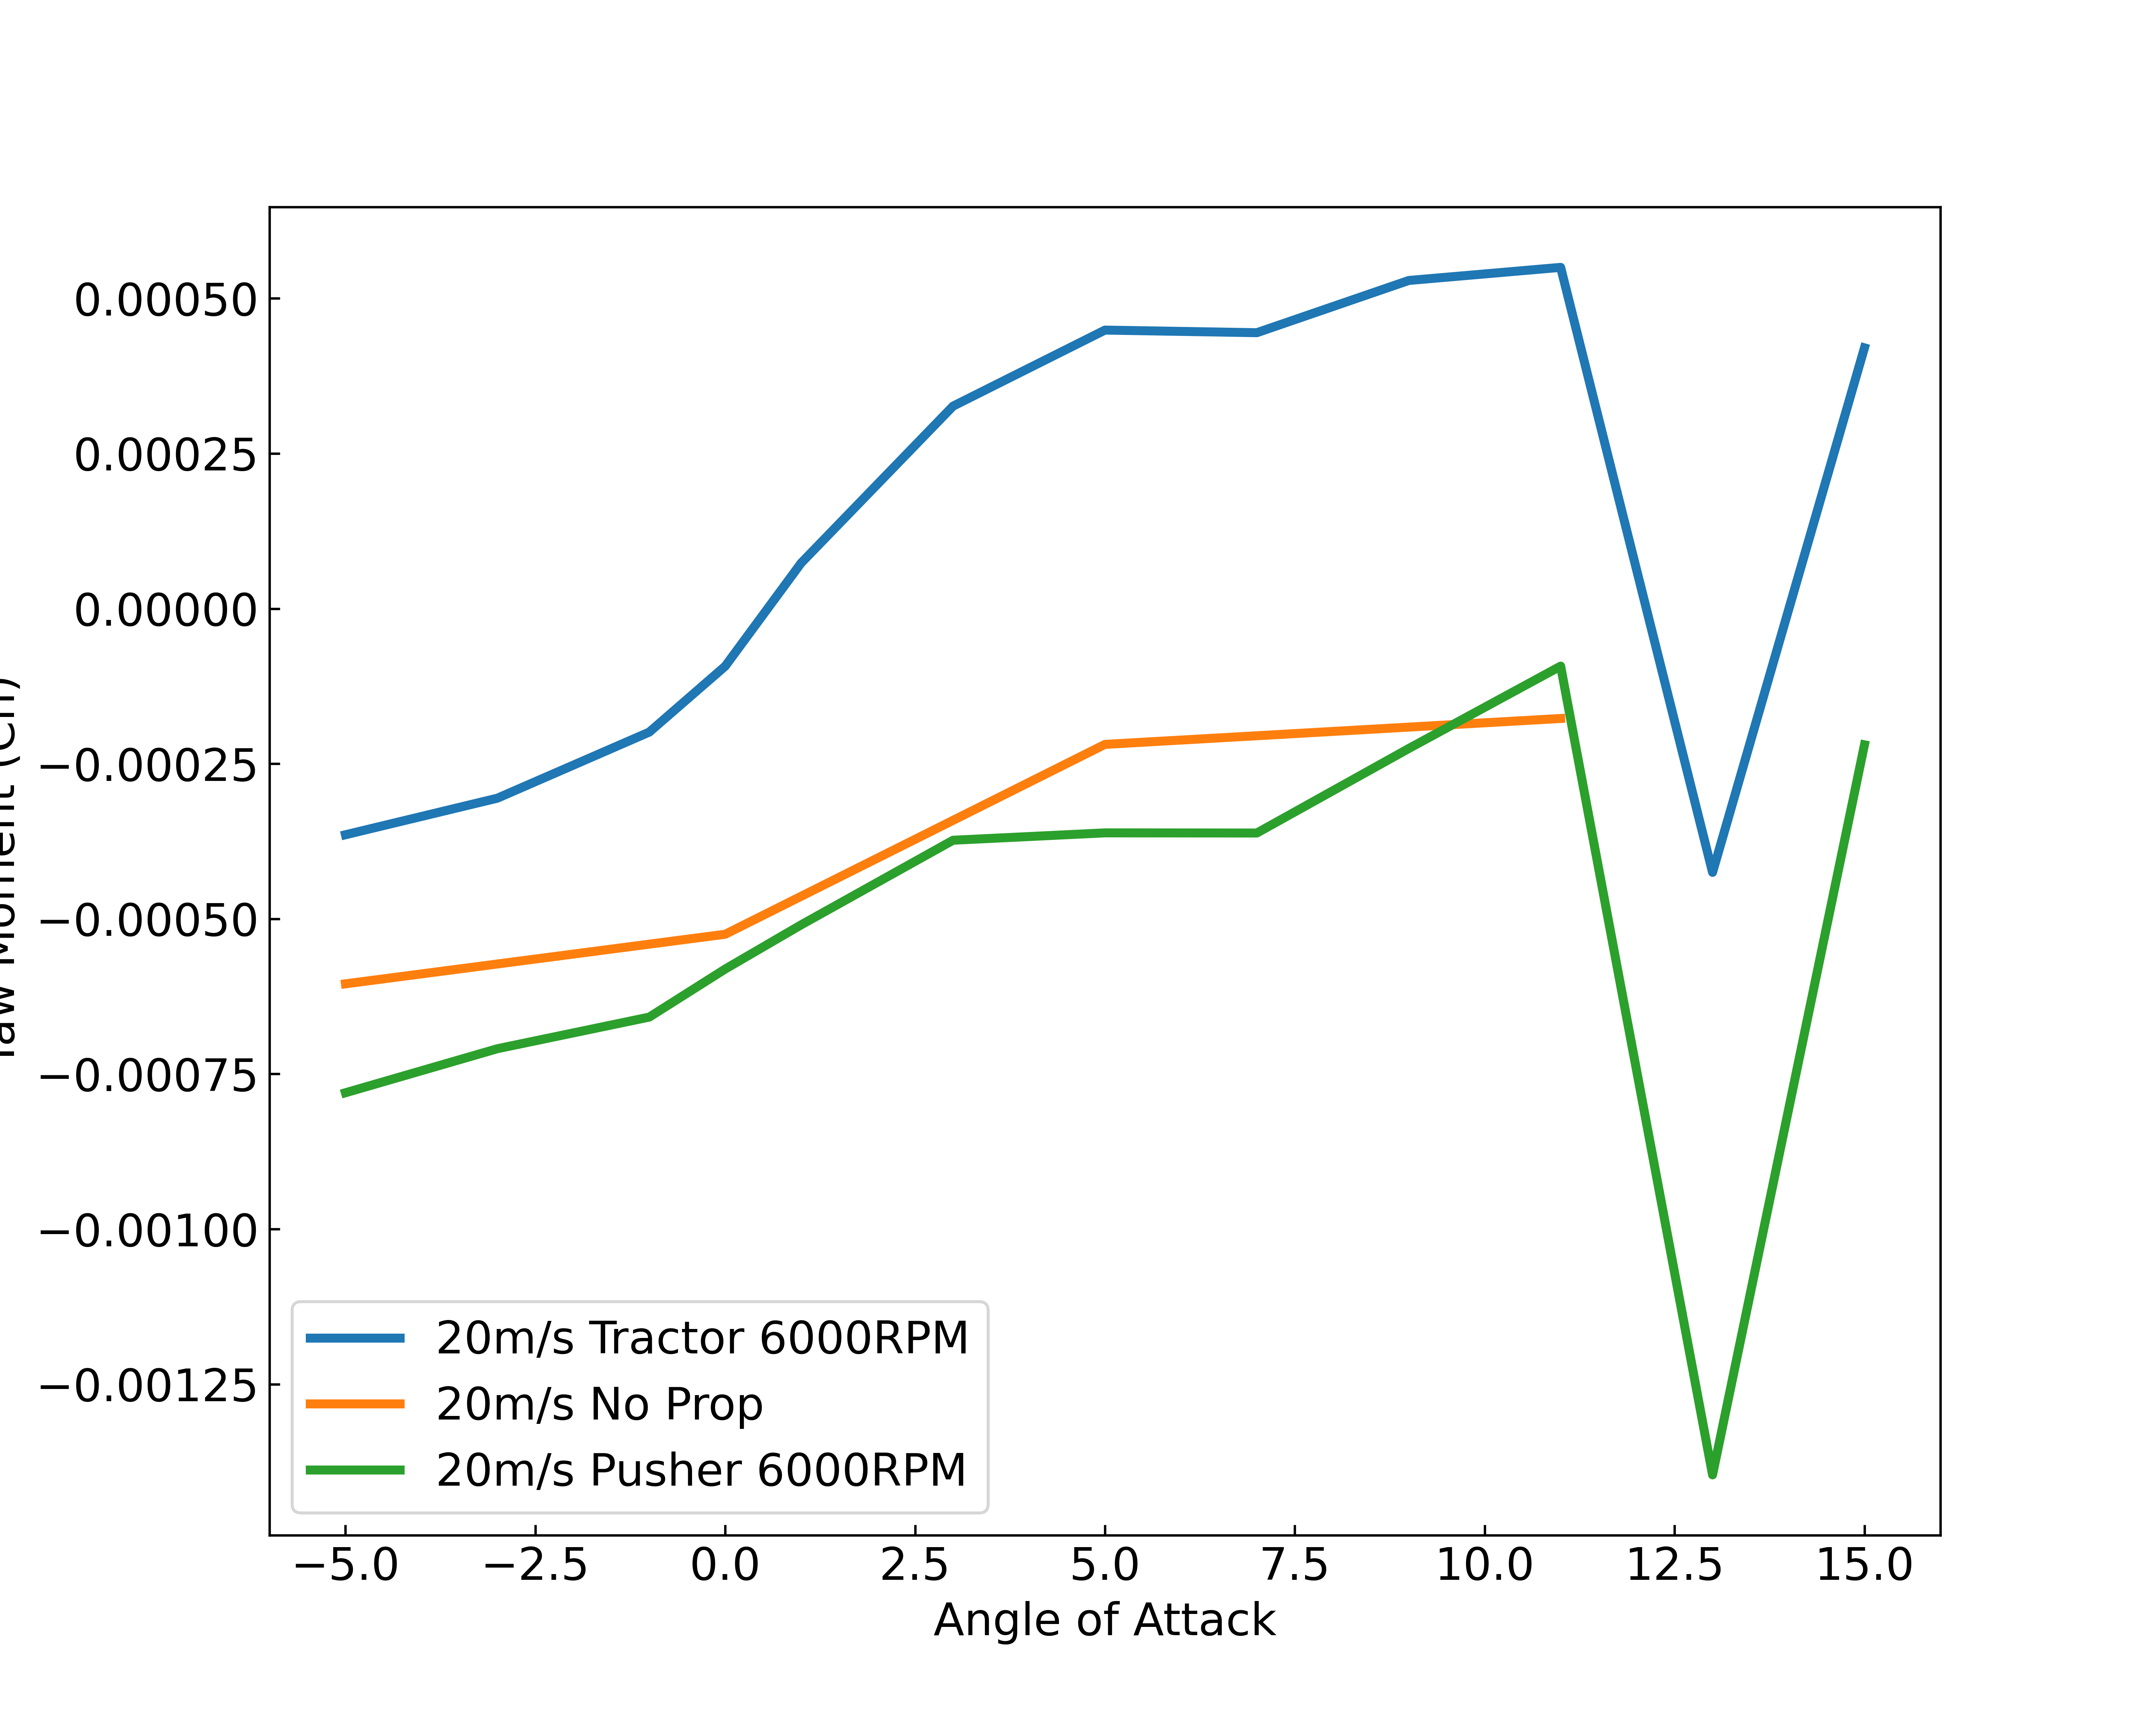
\includegraphics[width=\textwidth]{05_Results/Figs/Cn/20ms_6000RPM_Cn.png}
        \caption{Yawing Moment Coefficient at 20m/s airspeed and 6000RPM motor speed}
        \label{fig:Cn_20ms_6000}
    \end{subfigure}
    \begin{subfigure}[b]{0.467\textwidth}
        \centering
        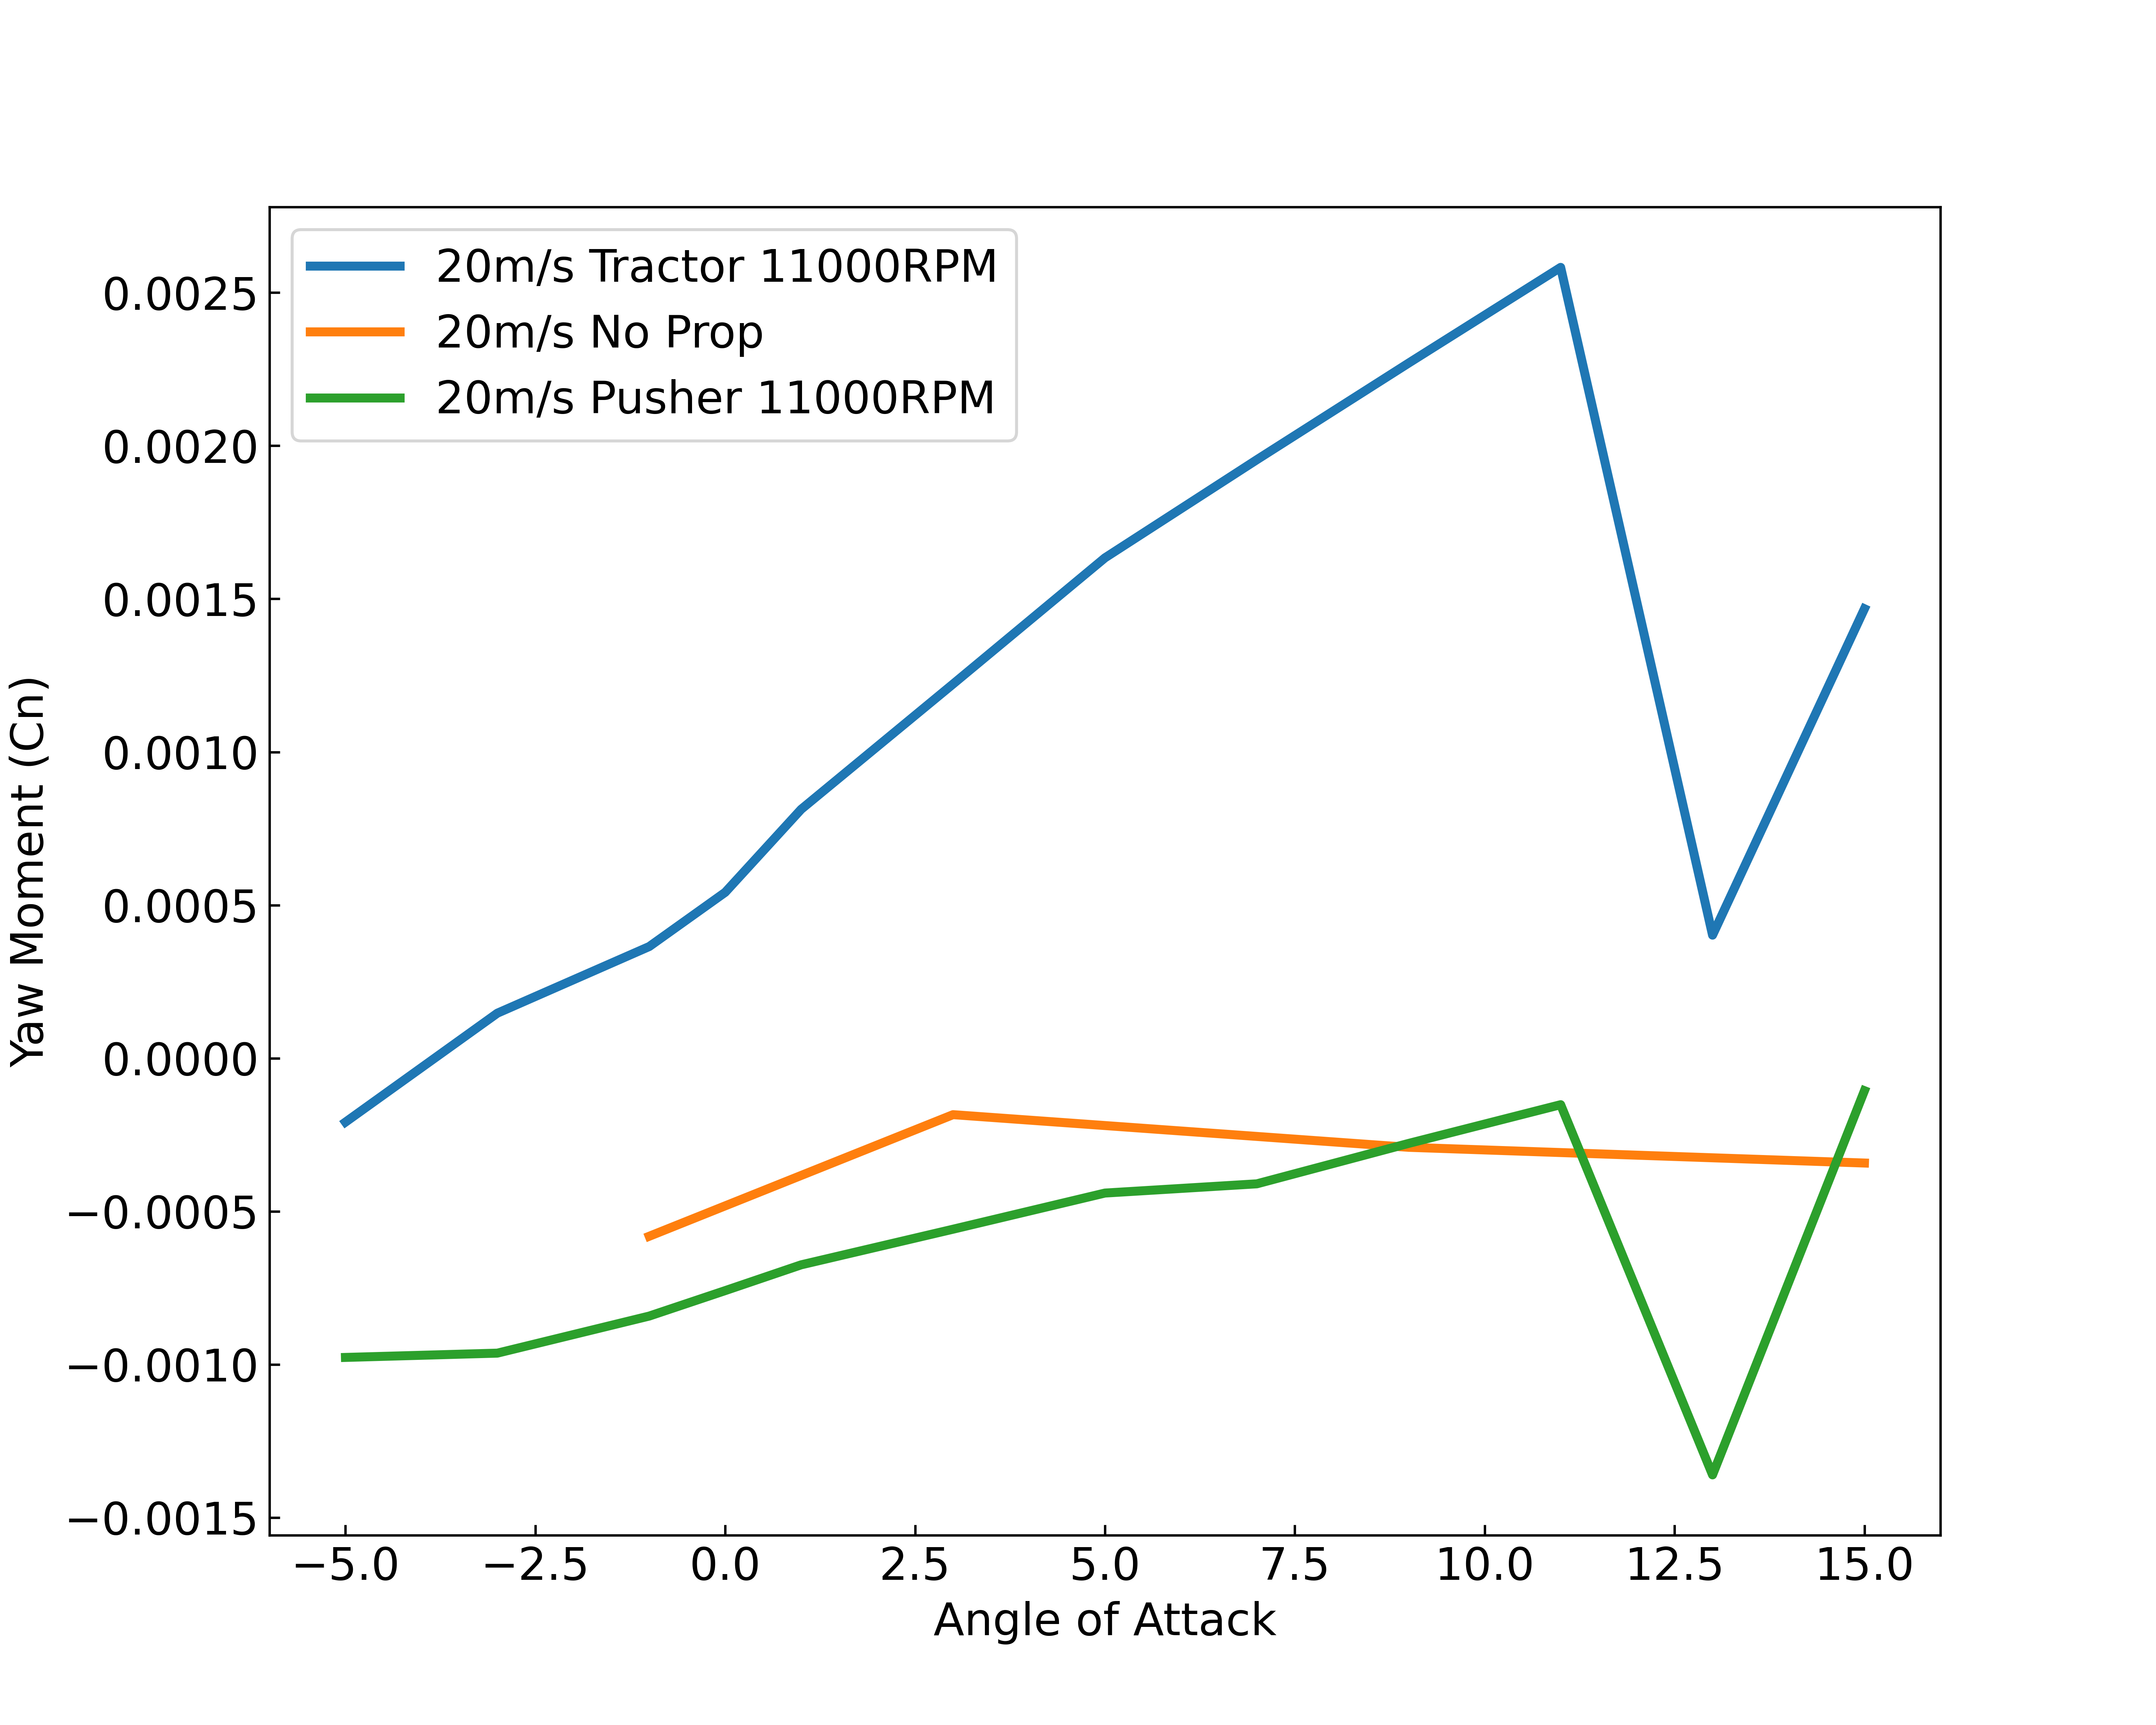
\includegraphics[width=\textwidth]{05_Results/Figs/Cn/20ms_11000RPM_Cn.png}
        \caption{Yawing Moment Coefficient at 20m/s airspeed and 11000RPM motor speed}
        \label{fig:Cn_20ms_11000}
    \end{subfigure}
\end{figure}




\subsection{Static Margin}
The static margin for all configurations shows that  For all airspeeds and propeller speeds tested the tractor configuration decreased the stability of the MAV with the exception of the 10m$s^{-1}$ at 6000RPM propeller speed. This is also seen more clearly in Table \ref{tab:staticMargin} as static margin decreases from -0.155 to -0.107 when comparing the no propeller and tractor configurations at 11000RPM and  10m$s^{-1}$. At 6000RPM propeller speed the tractor configuration became less stable when airspeed increased from 10m$s^{-1}$ to 20m$s^{-1}$, with the static margin decreasing from -0.116 to -0.106. This same trend was also seen for the pusher configuration at 6000RPM propeller speed, decreasing from -0.117 to -0.108. The opposite trend was seen when the propeller speed was increased to 11000RPM. The tractor and pusher configurations became more stable, increasing from -0.107 to -0.118 and from -0.156 to -0.173 respectively when  airspeed increased from 10m$s^{-1}$ to 20m$s^{-1}$. The no propeller configuration became more stable at all propeller speeds as the airspeed increased from 10m$s^{-1}$ to 20m$s^{-1}$.


\begin{tabular}{ |c|c|c|c| }
 \hline

 \hline
 Configuration & Airspeed (ms$^{-1}$ &  Propeller Speed (RPM) & Static Margin\\
 \hline
 Tractor & 10 & 6000 & -0.116 \\
 Tractor & 20 & 6000 & -0.106\\
No Propeller & 10 & 6000 & -0.100\\
  No Propeller & 20 & 6000 & -0.107 \\
 Pusher & 10 & 6000 & -0.117 \\
  Pusher & 20 & 6000 & -0.108 \\
  \hline
 Tractor & 10 & 11000 & -0.107 \\
 Tractor & 20 & 11000 & -0.118\\
 No Propeller & 10 & 11000 & -0.155\\
 No Propeller& 20 & 11000 & -0.159\\
 Pusher & 10 & 11000 & -0.156 \\
 Pusher & 20 & 11000 & -0.173 \\
 \hline
 \label{tab:staticMargin}
\end{tabular}



\begin{figure}[H]
    \centering
    \begin{subfigure}[b]{0.467\textwidth}
        \centering
        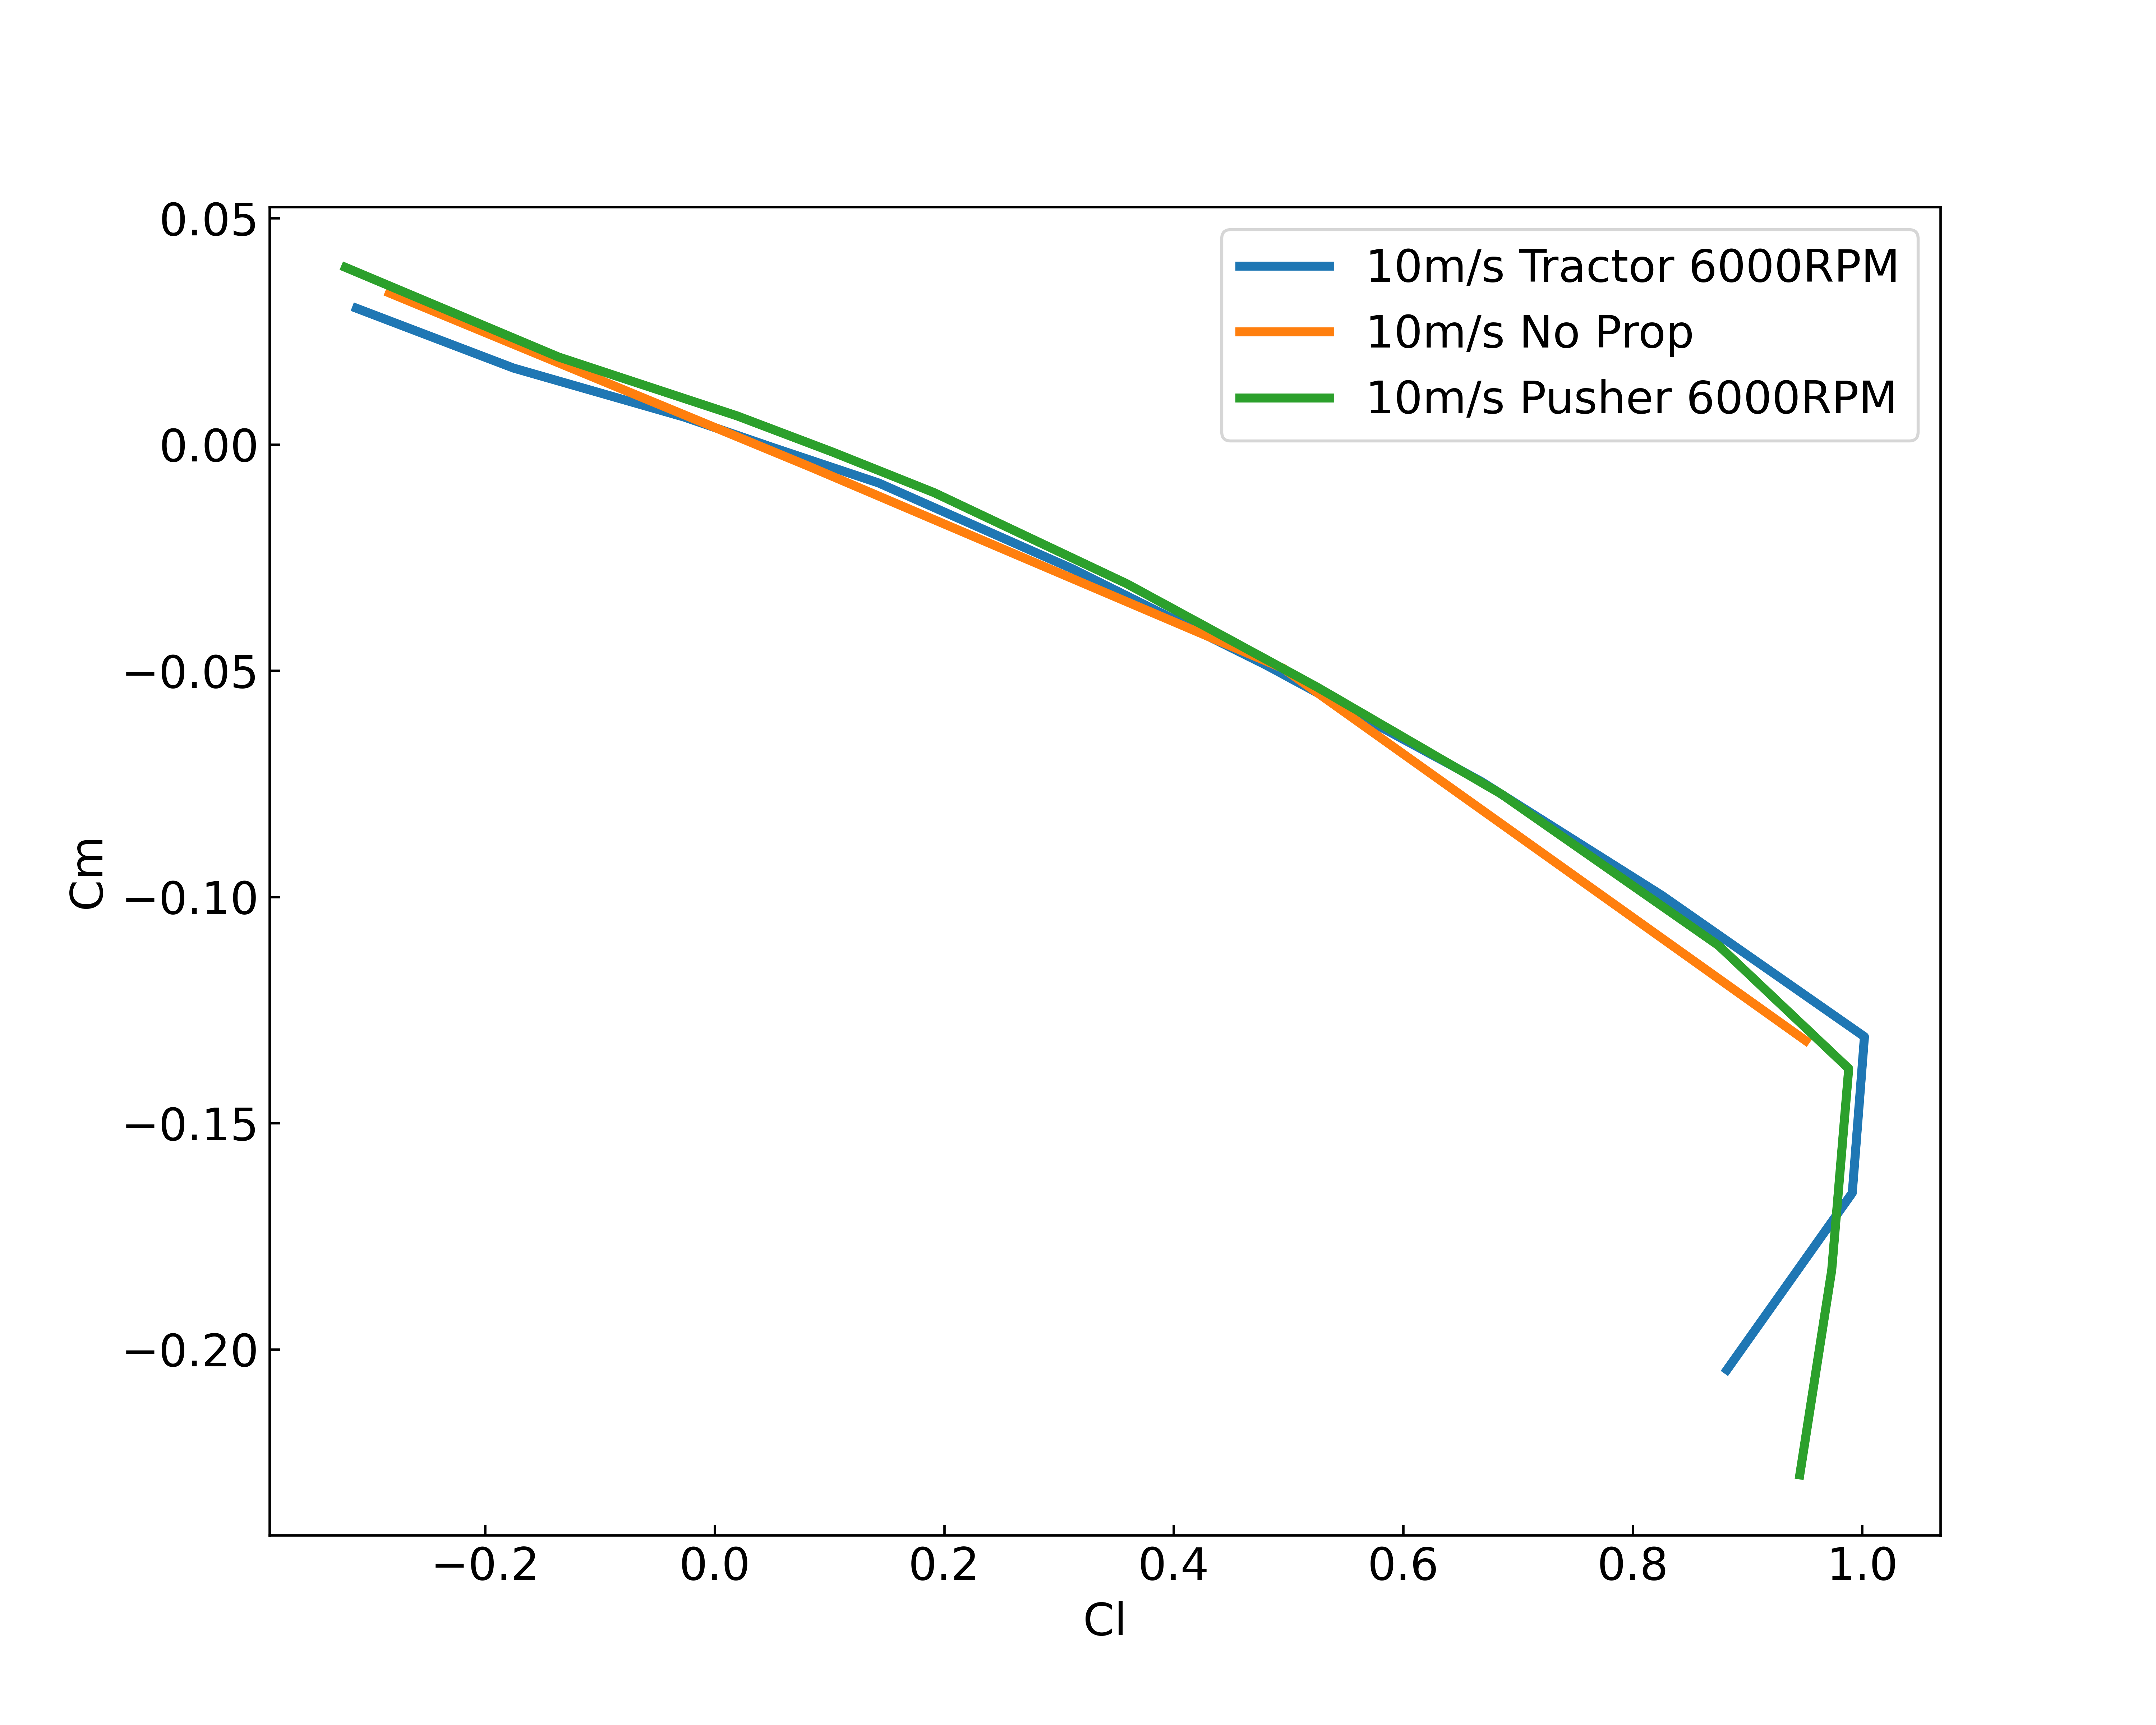
\includegraphics[width=\textwidth]{05_Results/Figs/ClCm/10ms_6000RPM_CmCl.png}
        \caption{Rolling Moment Coefficient at 10m/s airspeed and 6000RPM motor speed}
        \label{fig:CmCl_10ms_6000}
    \end{subfigure}
    \begin{subfigure}[b]{0.467\textwidth}
        \centering
        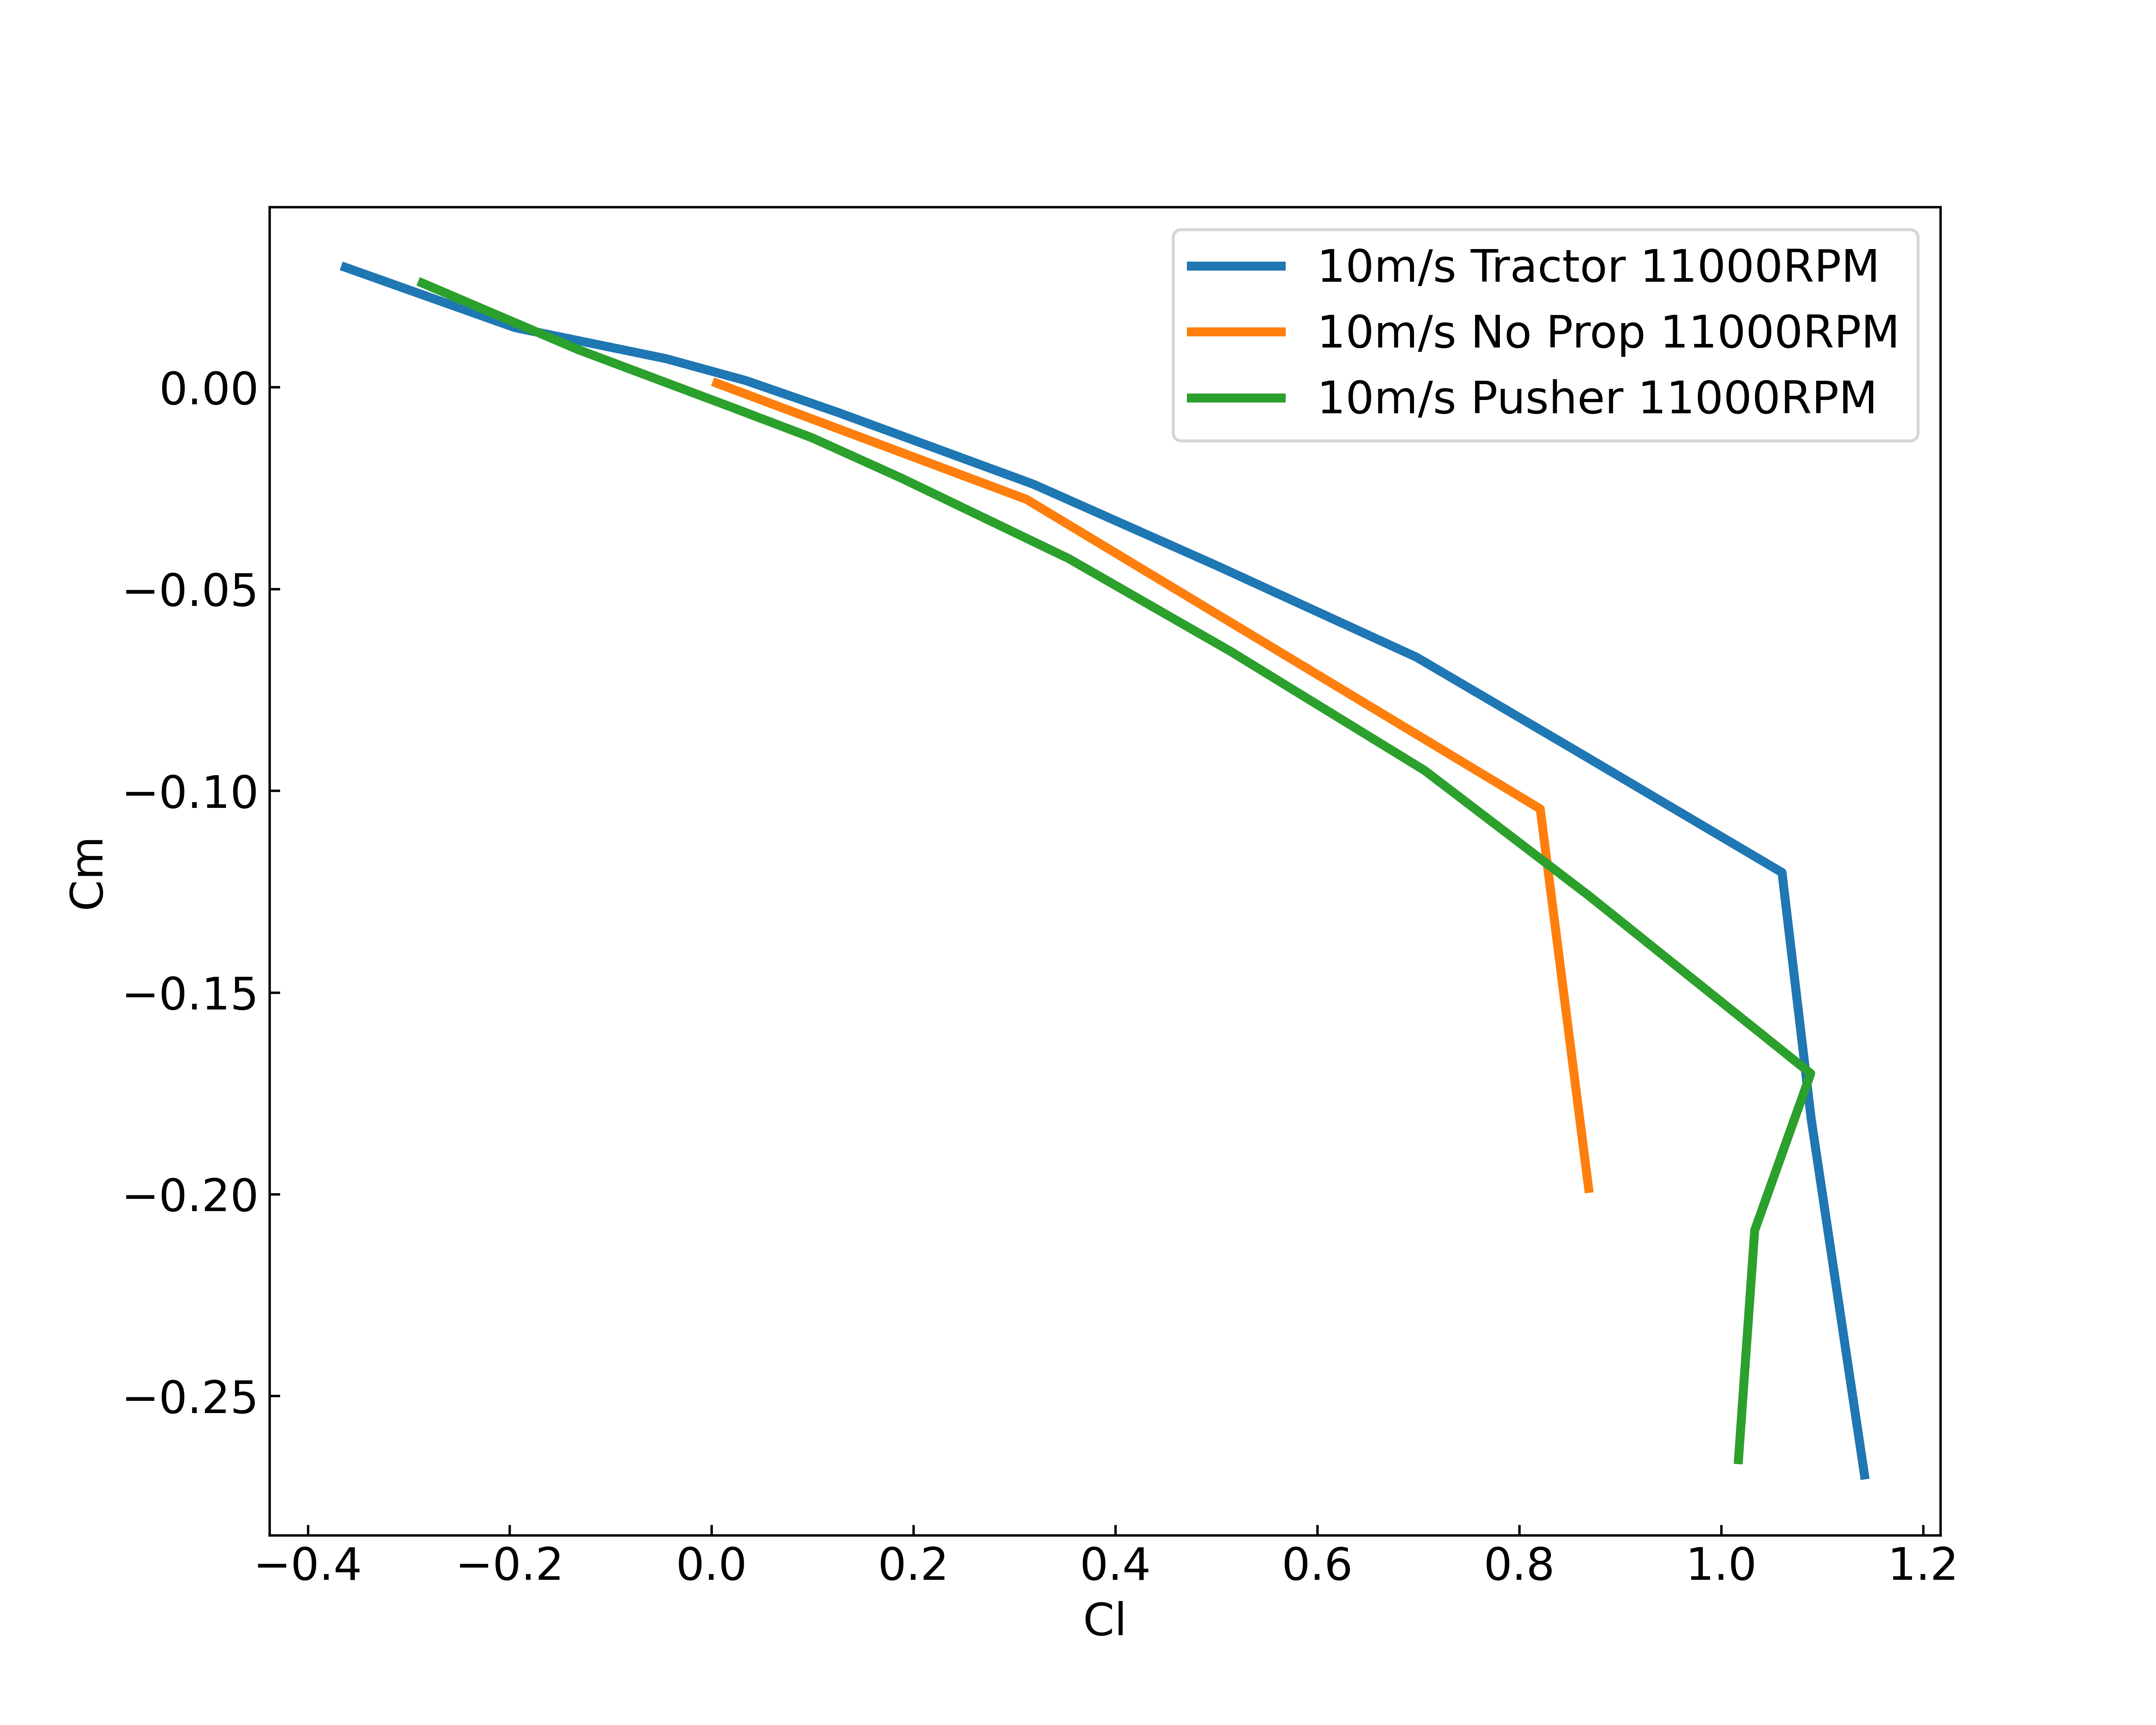
\includegraphics[width=\textwidth]{05_Results/Figs/ClCm/10ms_11000RPM_CmCl.png}
        \caption{Rolling Moment Coefficient at 10m/s airspeed and 11000RPM motor speed}
        \label{fig:CmCl_10ms_11000}
    \end{subfigure}
    \begin{subfigure}[b]{0.467\textwidth}
        \centering
        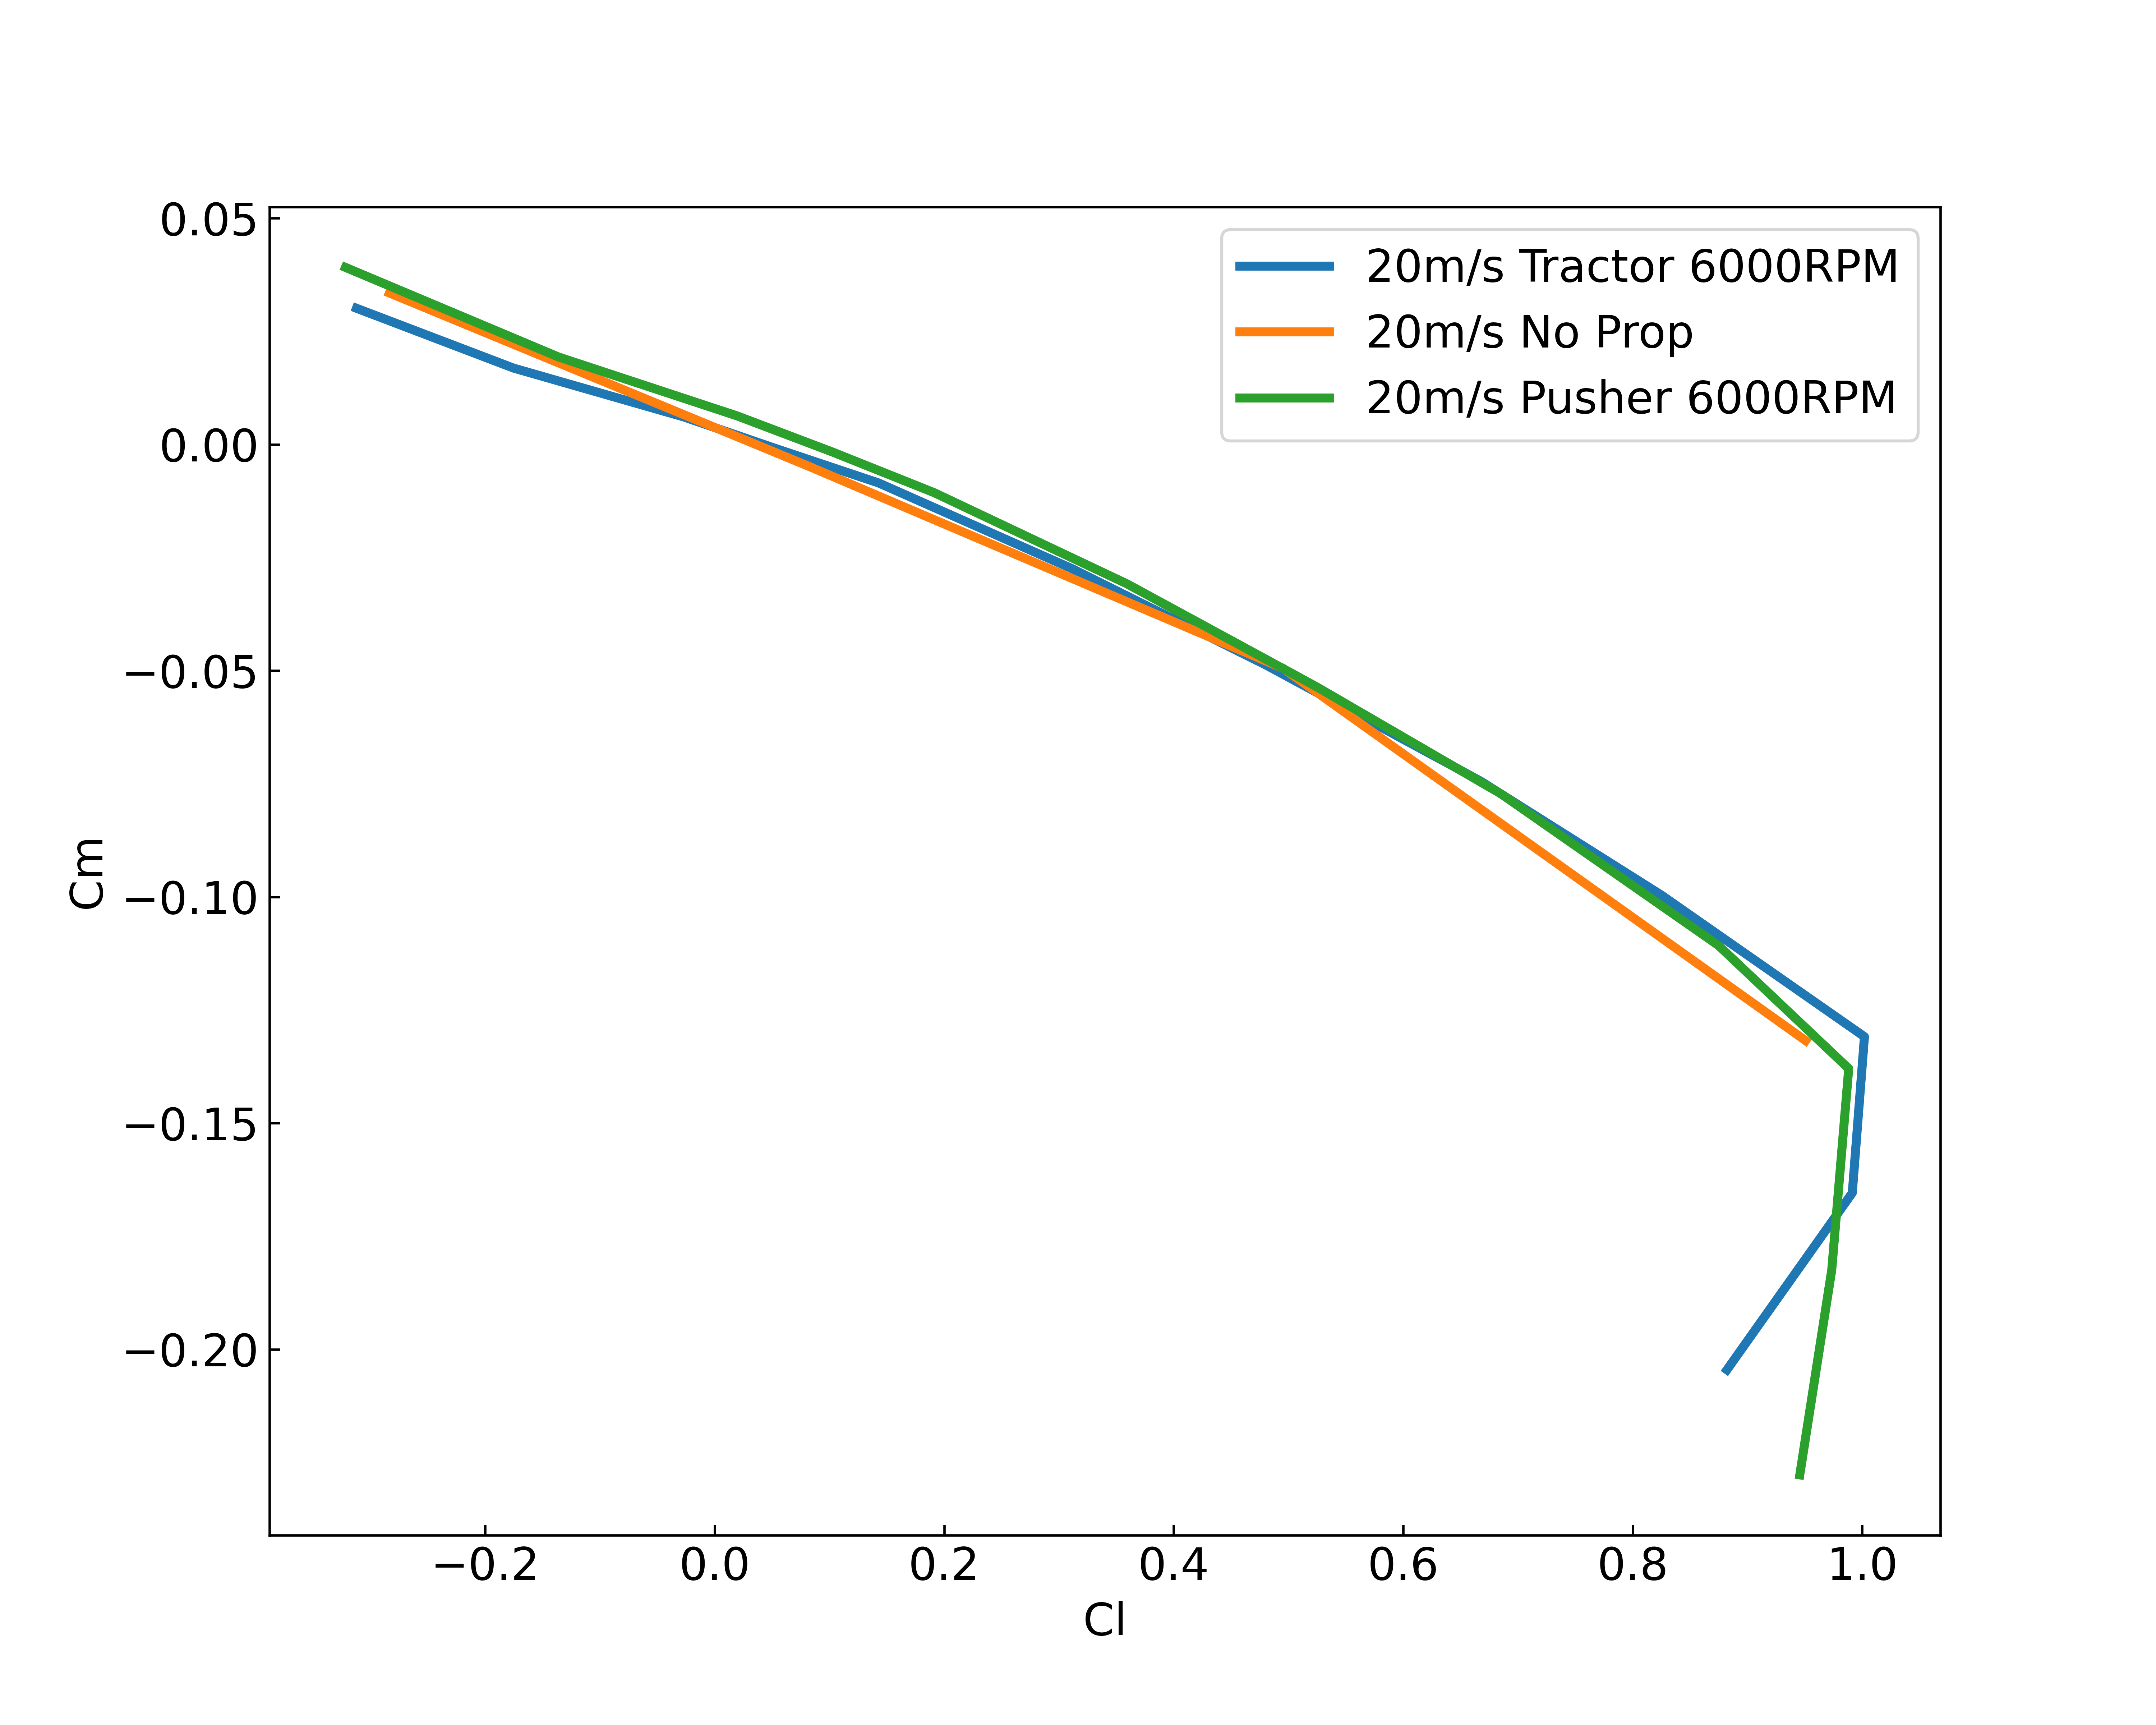
\includegraphics[width=\textwidth]{05_Results/Figs/ClCm/20ms_6000RPM_CmCl.png}
        \caption{Rolling Moment Coefficient at 20m/s airspeed and 6000RPM motor speed}
        \label{fig:CmCl_20ms_6000}
    \end{subfigure}
    \begin{subfigure}[b]{0.467\textwidth}
        \centering
        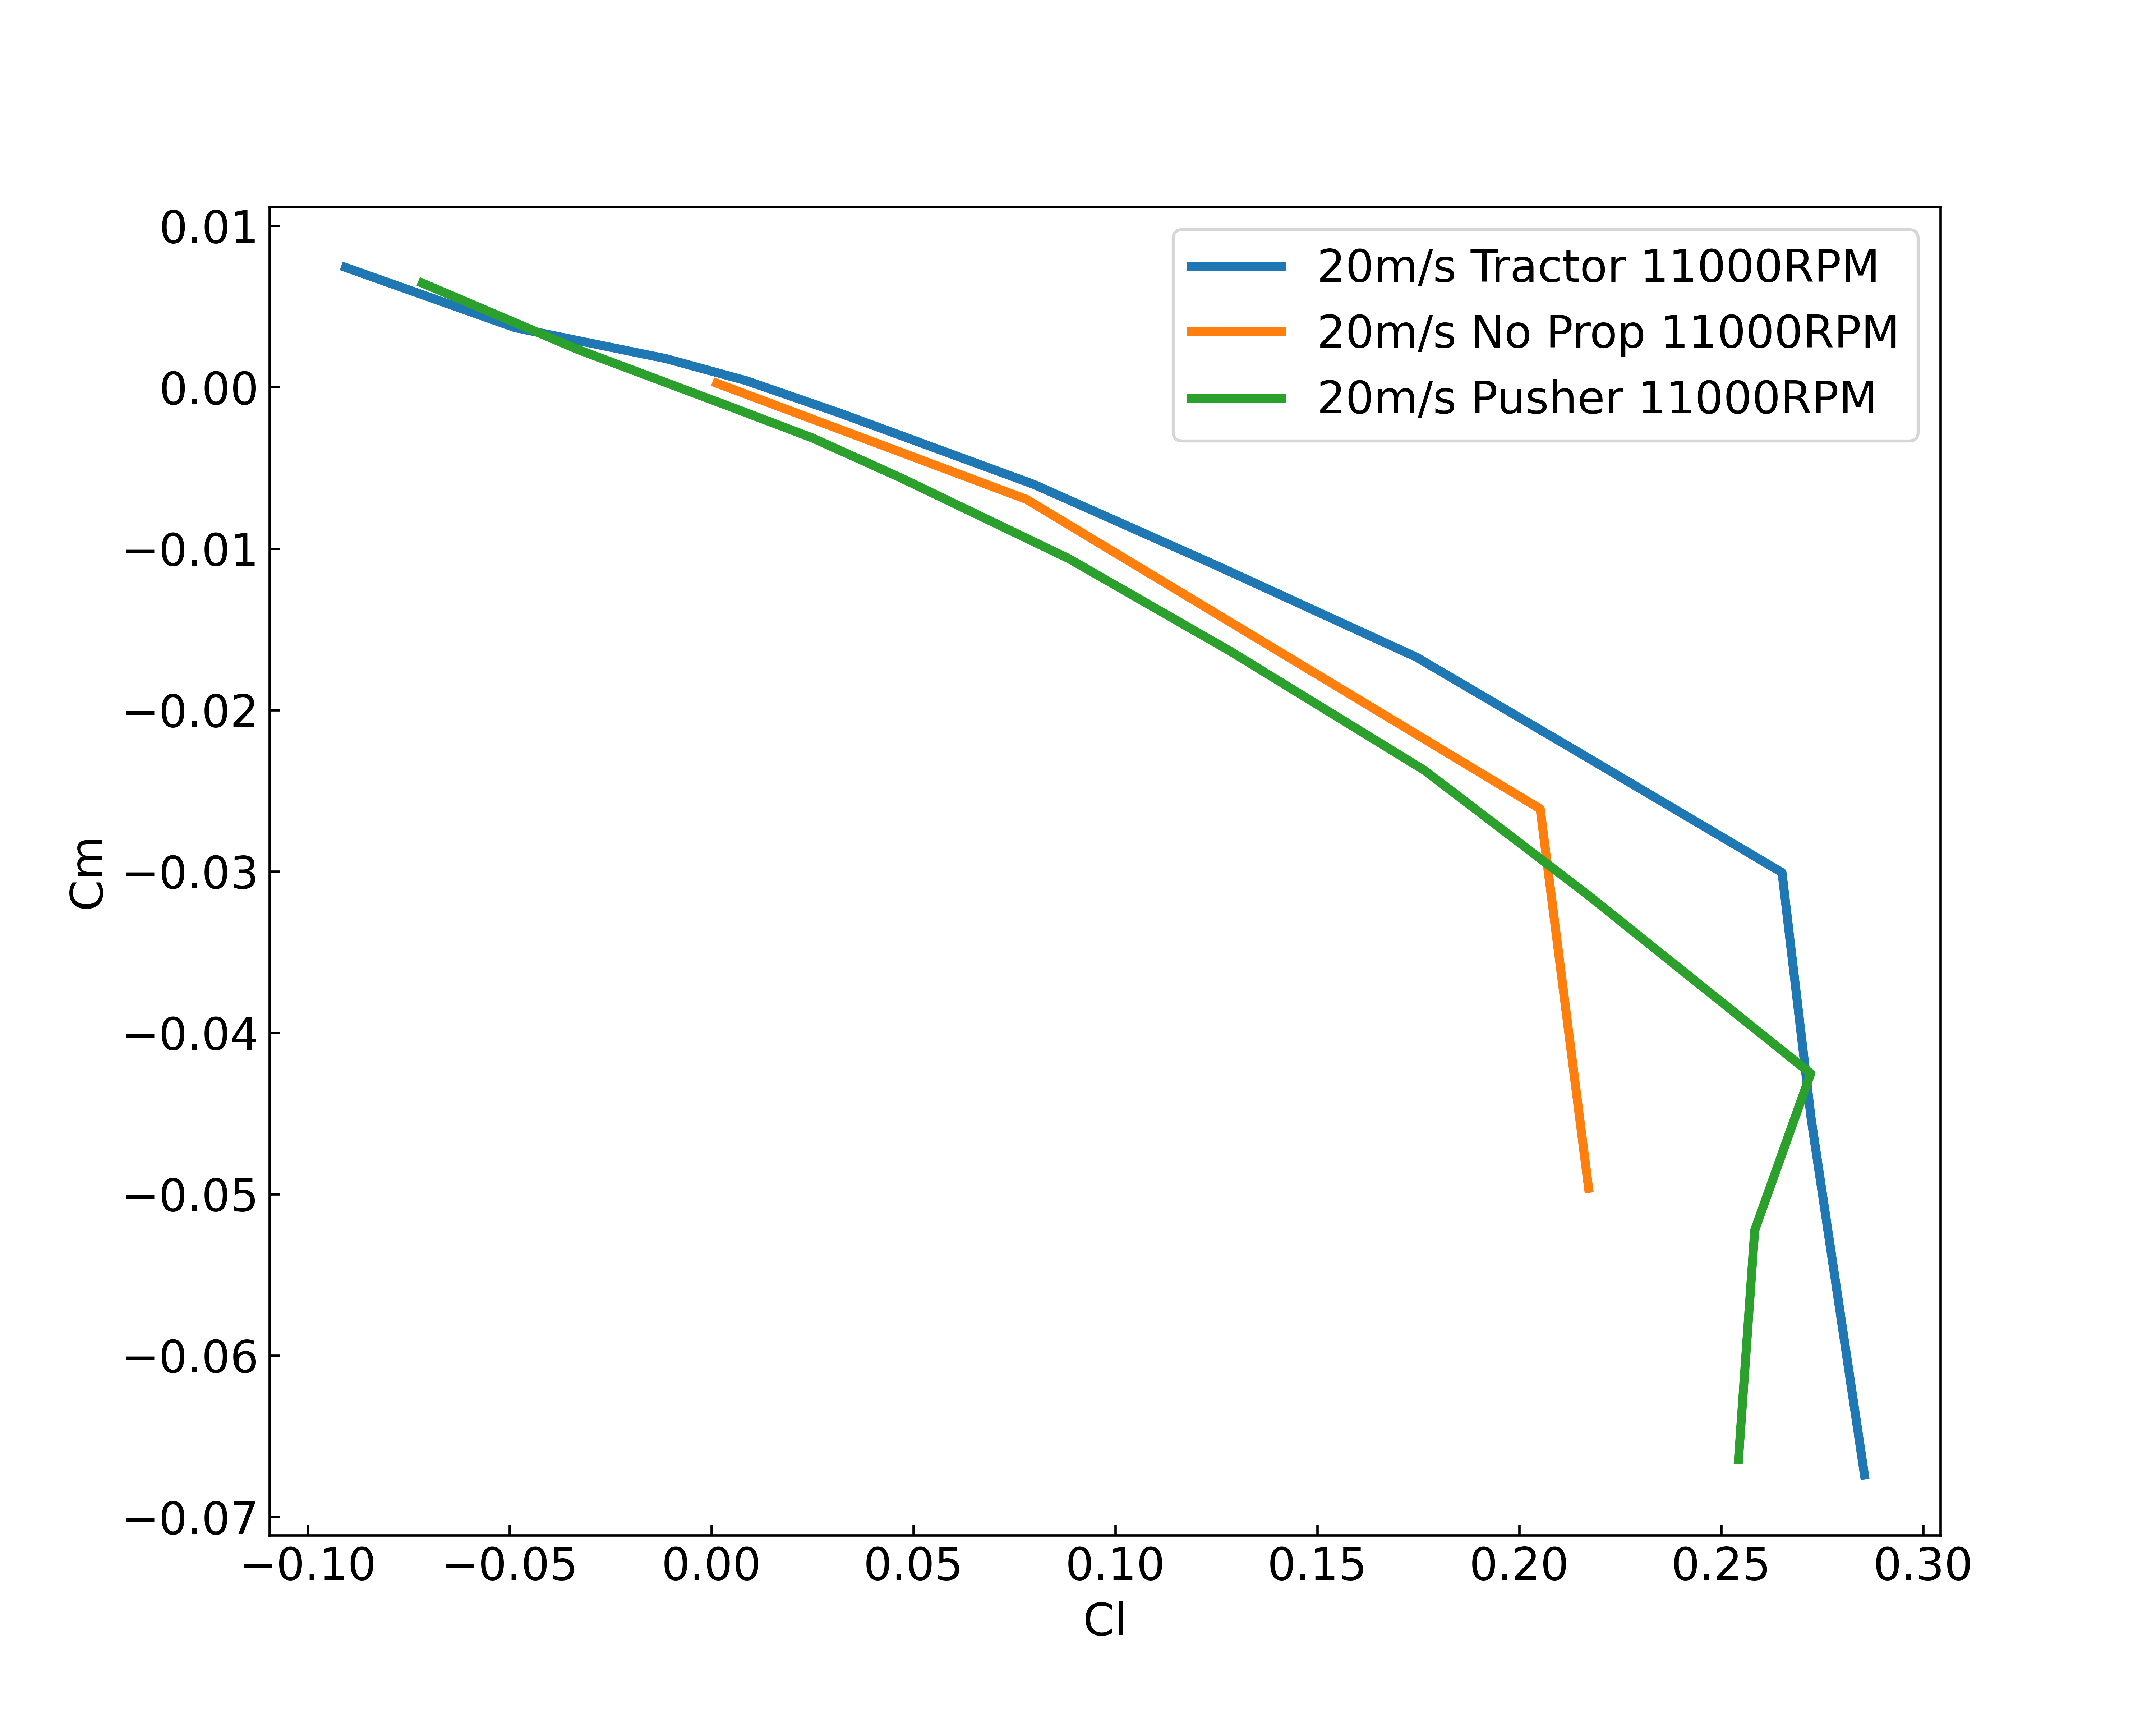
\includegraphics[width=\textwidth]{05_Results/Figs/ClCm/20ms_11000RPM_CmCl.png}
        \caption{Rolling Moment Coefficient at 20m/s airspeed and 11000RPM motor speed}
        \label{fig:CmCl_20ms_11000}
    \end{subfigure}
\end{figure}


\section{VAP 3.5 Validation}
Low speed aerodynamics generally see complex flow distributions and phenomena as dicussed in Sections \ref{sec:Reynolds} and \ref{sec:Reynolds2}. In order to evaluate the usage of VAP 3.5 for the wind tunnel tests conducted, a wing validation and model validation was performed with comparison to the GenMAV model which has been previously evaluated with the Athena Vortex Lattice (AVL) method in order to estimate the stability derivatives and moments of the GenMAV. 

\subsection{Wing Validation}
A wing validation against Fluent CFD results is given in Figures \ref{fig:wing0300} to Figure \ref{fig:001000b} \cite{}. This data was taken at a Reynolds number of 2.32 $\times 10^{5}$ at a freestream velocity of 20$m/s$ and density 1.225$kg/m^3$. 

\begin{figure}[H]
     \centering
     \begin{subfigure}[b]{0.45\textwidth}
         \centering
         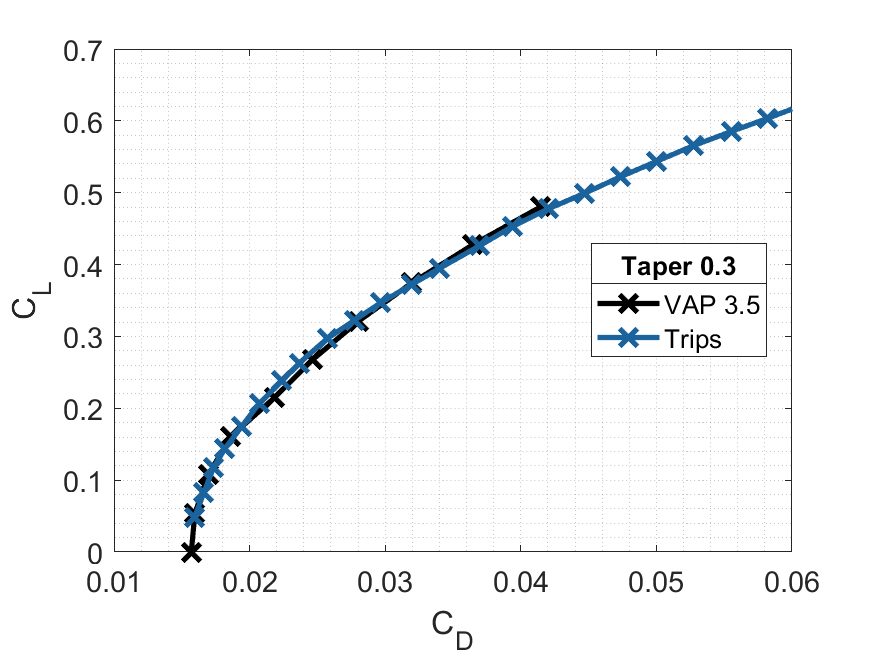
\includegraphics[width=\textwidth]{05_Results/Figs/VAP/genMAV/taper3a.png}
         \caption{}
         \label{fig:wing0300}

     \end{subfigure}
     \hfill
     \begin{subfigure}[b]{0.45\textwidth}
         \centering
         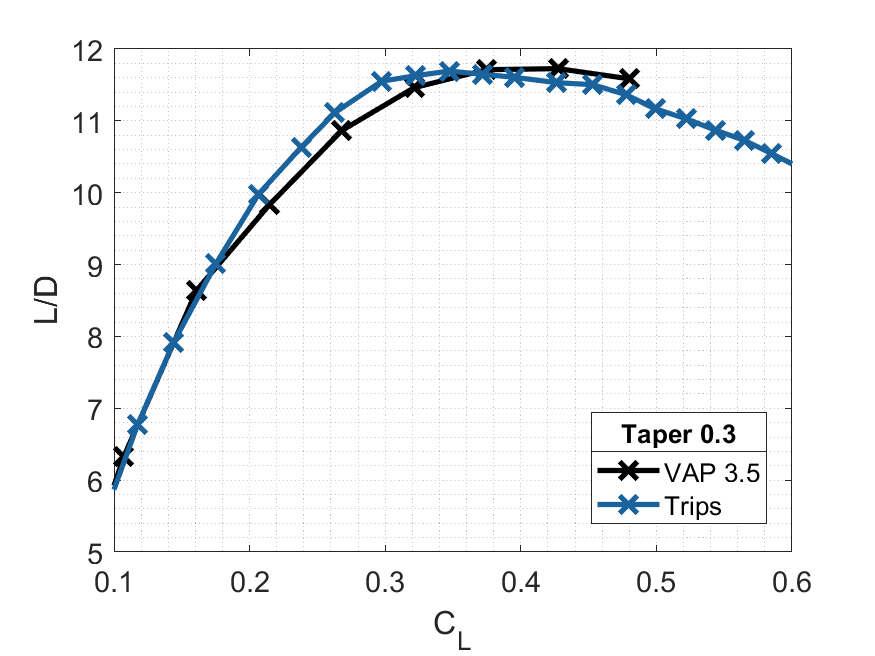
\includegraphics[width=\textwidth]{05_Results/Figs/VAP/genMAV/taper3b.png}
         \caption{}
         \label{fig:wing0300b}
      
     \end{subfigure}
     \hfill

        
\end{figure}


\begin{figure}[H]
     \centering
     \begin{subfigure}[b]{0.45\textwidth}
         \centering
         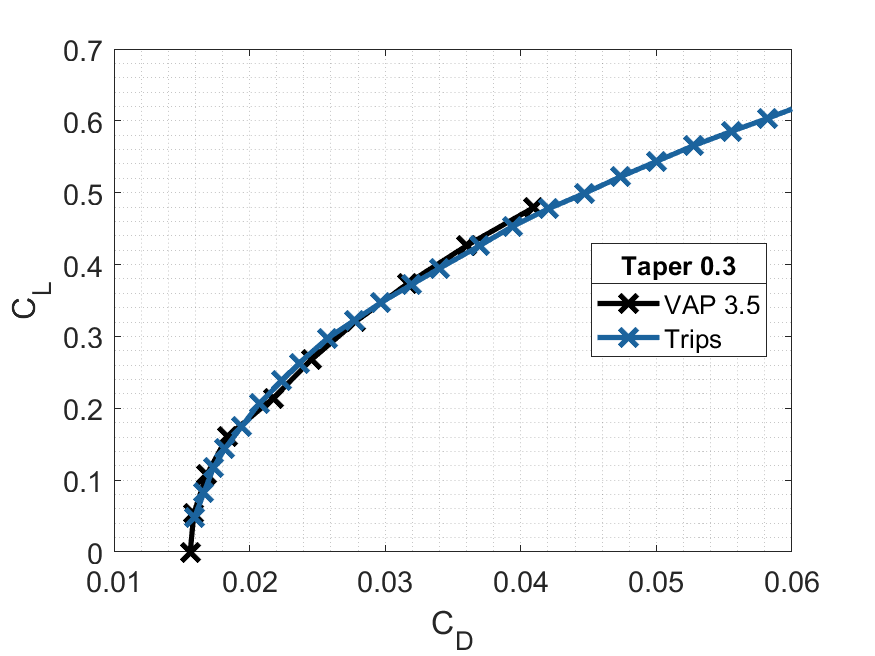
\includegraphics[width=\textwidth]{05_Results/Figs/VAP/genMAV/taper5a.png}

     \end{subfigure}
     \hfill
     \begin{subfigure}[b]{0.45\textwidth}
         \centering
         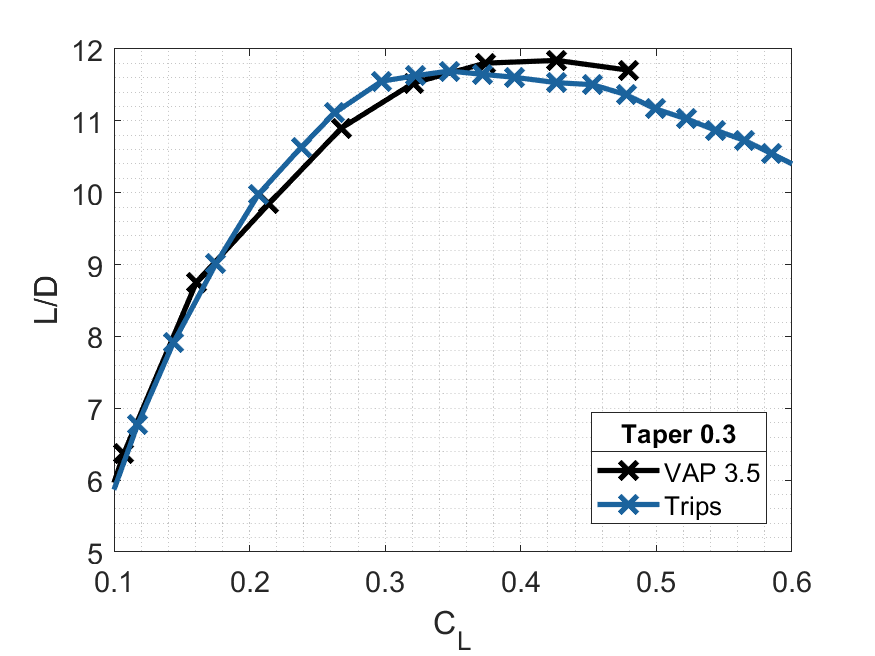
\includegraphics[width=\textwidth]{05_Results/Figs/VAP/genMAV/taper5b.png}
      
     \end{subfigure}
     \hfill

        
\end{figure}


\begin{figure}[H]
     \centering
     \begin{subfigure}[b]{0.45\textwidth}
         \centering
         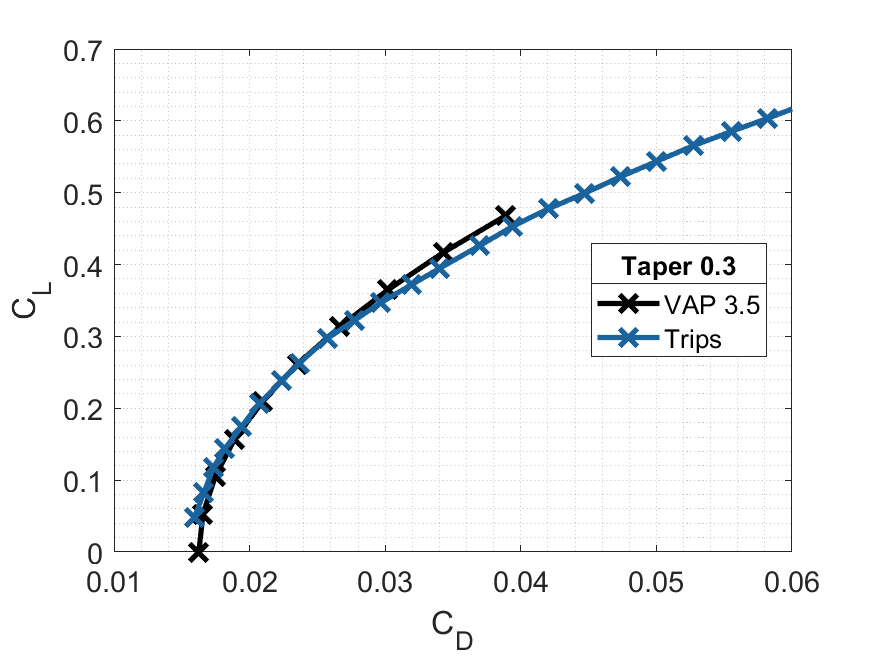
\includegraphics[width=\textwidth]{05_Results/Figs/VAP/genMAV/taper10a.png}

     \end{subfigure}
     \hfill
     \begin{subfigure}[b]{0.45\textwidth}
         \centering
         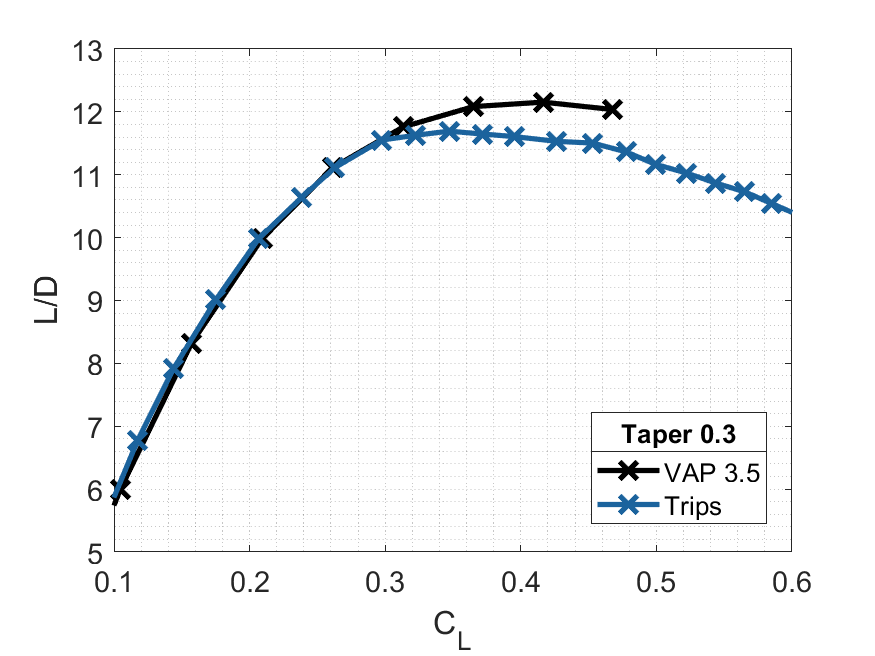
\includegraphics[width=\textwidth]{05_Results/Figs/VAP/genMAV/taper10b.png}
         \caption{}
         
      \label{fig:001000b}
     \end{subfigure}
     \hfill

        
\end{figure}


\subsection{GenMAV model validation}


\begin{figure}[H]
     \centering
     \begin{subfigure}[b]{0.45\textwidth}
          \centering
        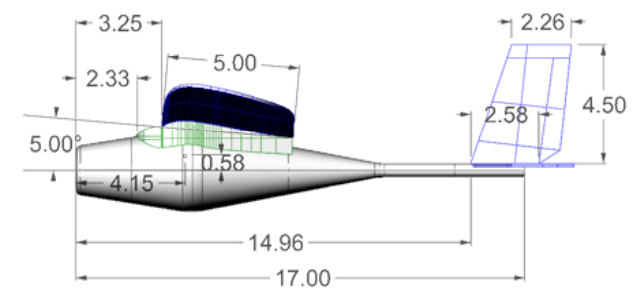
\includegraphics[width=\textwidth]{05_Results/Figs/VAP/genMAV/dimensions.png}
            \label{fig:genMAVDimensions}

     \end{subfigure}
     \hfill
     \begin{subfigure}[b]{0.45\textwidth}
                \centering
            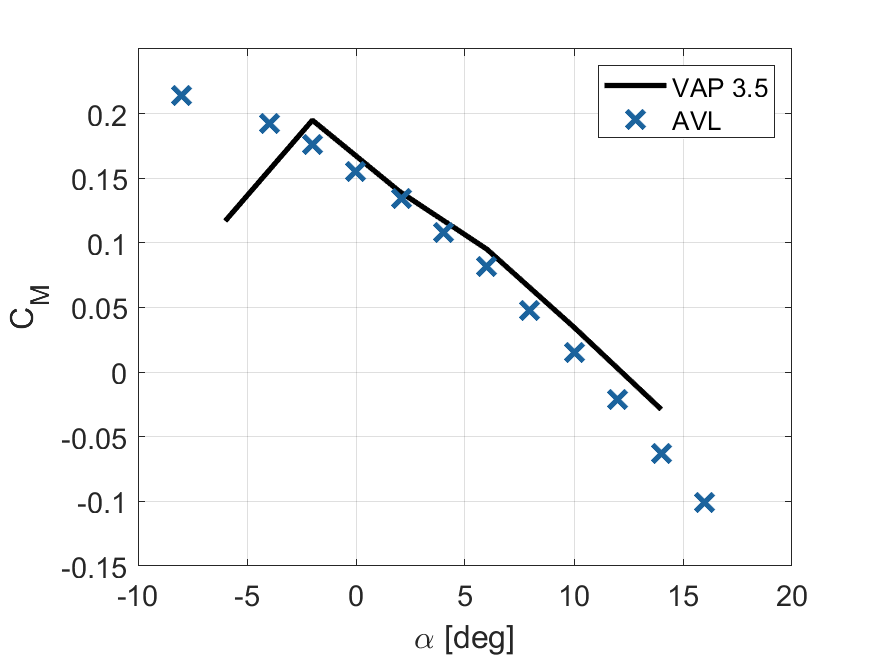
\includegraphics[width=\textwidth]{05_Results/Figs/VAP/genMAV/GenMAVModelValidation1.png}
             \label{fig:genMAV_Cm}
              \caption{}
     \end{subfigure}
     \hfill

        
\end{figure}


\begin{figure}[H]
     \centering
     \begin{subfigure}[b]{0.45\textwidth}
            \centering
         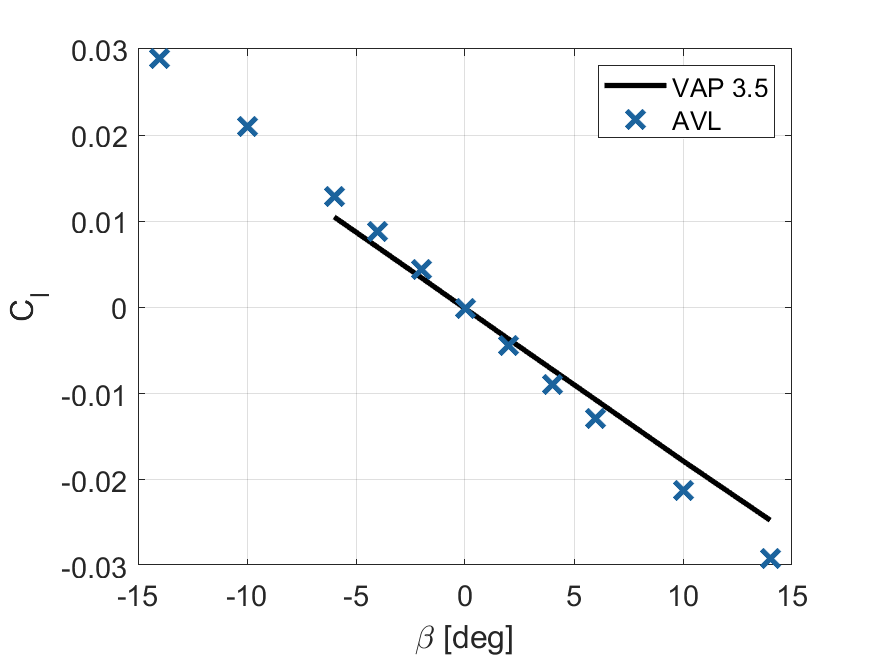
\includegraphics[width=\textwidth]{05_Results/Figs/VAP/genMAV/GenMAVModelValidation2.png}
         \label{fig:genMAV_Cl_roll}
         \caption{}

     \end{subfigure}
     \hfill
     \begin{subfigure}[b]{0.45\textwidth}
               \centering
         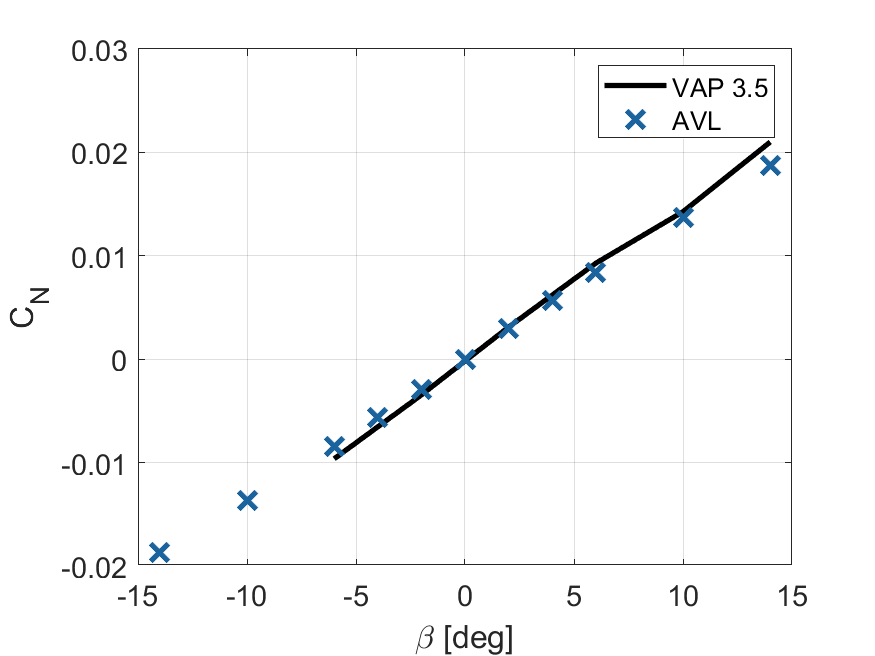
\includegraphics[width=\textwidth]{05_Results/Figs/VAP/genMAV/GenMAVModelValidation3.png}
         \label{fig:genMAV_Cn}
         \caption{}
     \end{subfigure}
     \hfill
\end{figure}



\begin{figure}[H]
    \centering
    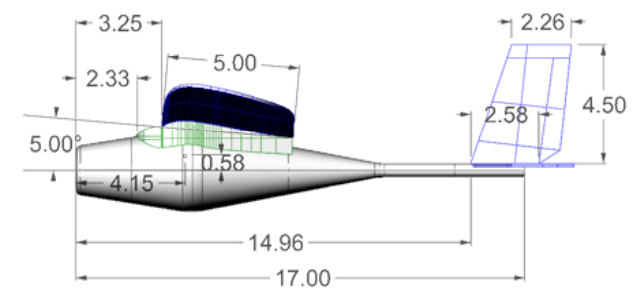
\includegraphics[width=0.5\textwidth]{05_Results/Figs/VAP/genMAV/dimensions.png}
    \label{fig:genMAVDimensions}
\end{figure}

\begin{figure}[H]
         \centering
         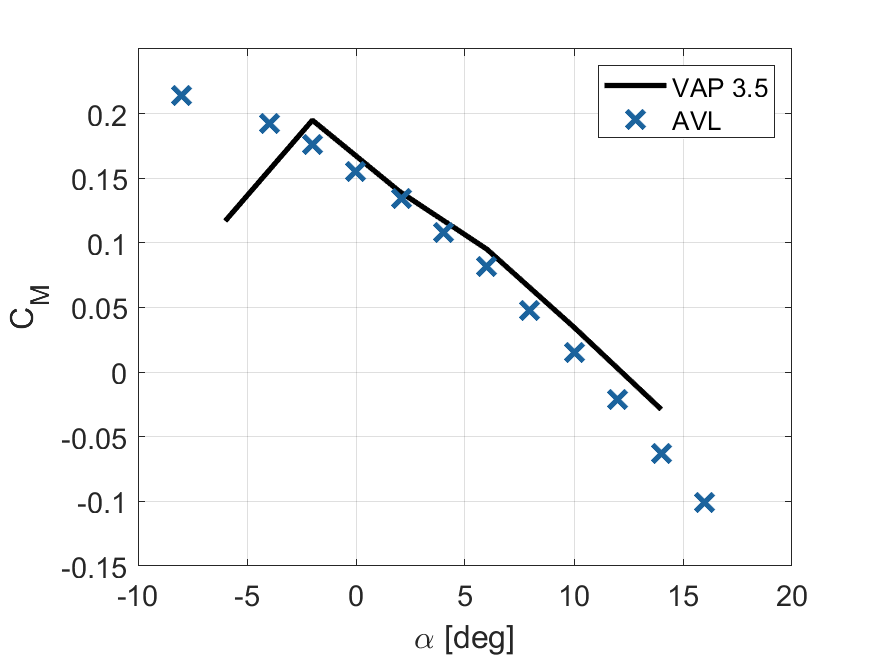
\includegraphics[width=0.5\textwidth]{05_Results/Figs/VAP/genMAV/GenMAVModelValidation1.png}
         \label{fig:genMAV_Cm}
         \caption{}
\end{figure}

% \begin{figure}[H]
       
% \end{figure}

% \begin{figure}
       
% \end{figure}

\subsection{Validation of Wind Tunnel Results with VAP 3.5}
side forces and moments still in testing for VAP 3.5

\subsubsection{No Propeller Configuration}


\begin{figure}[H]
    \centering
    \begin{subfigure}[b]{0.467\textwidth}
        \centering
        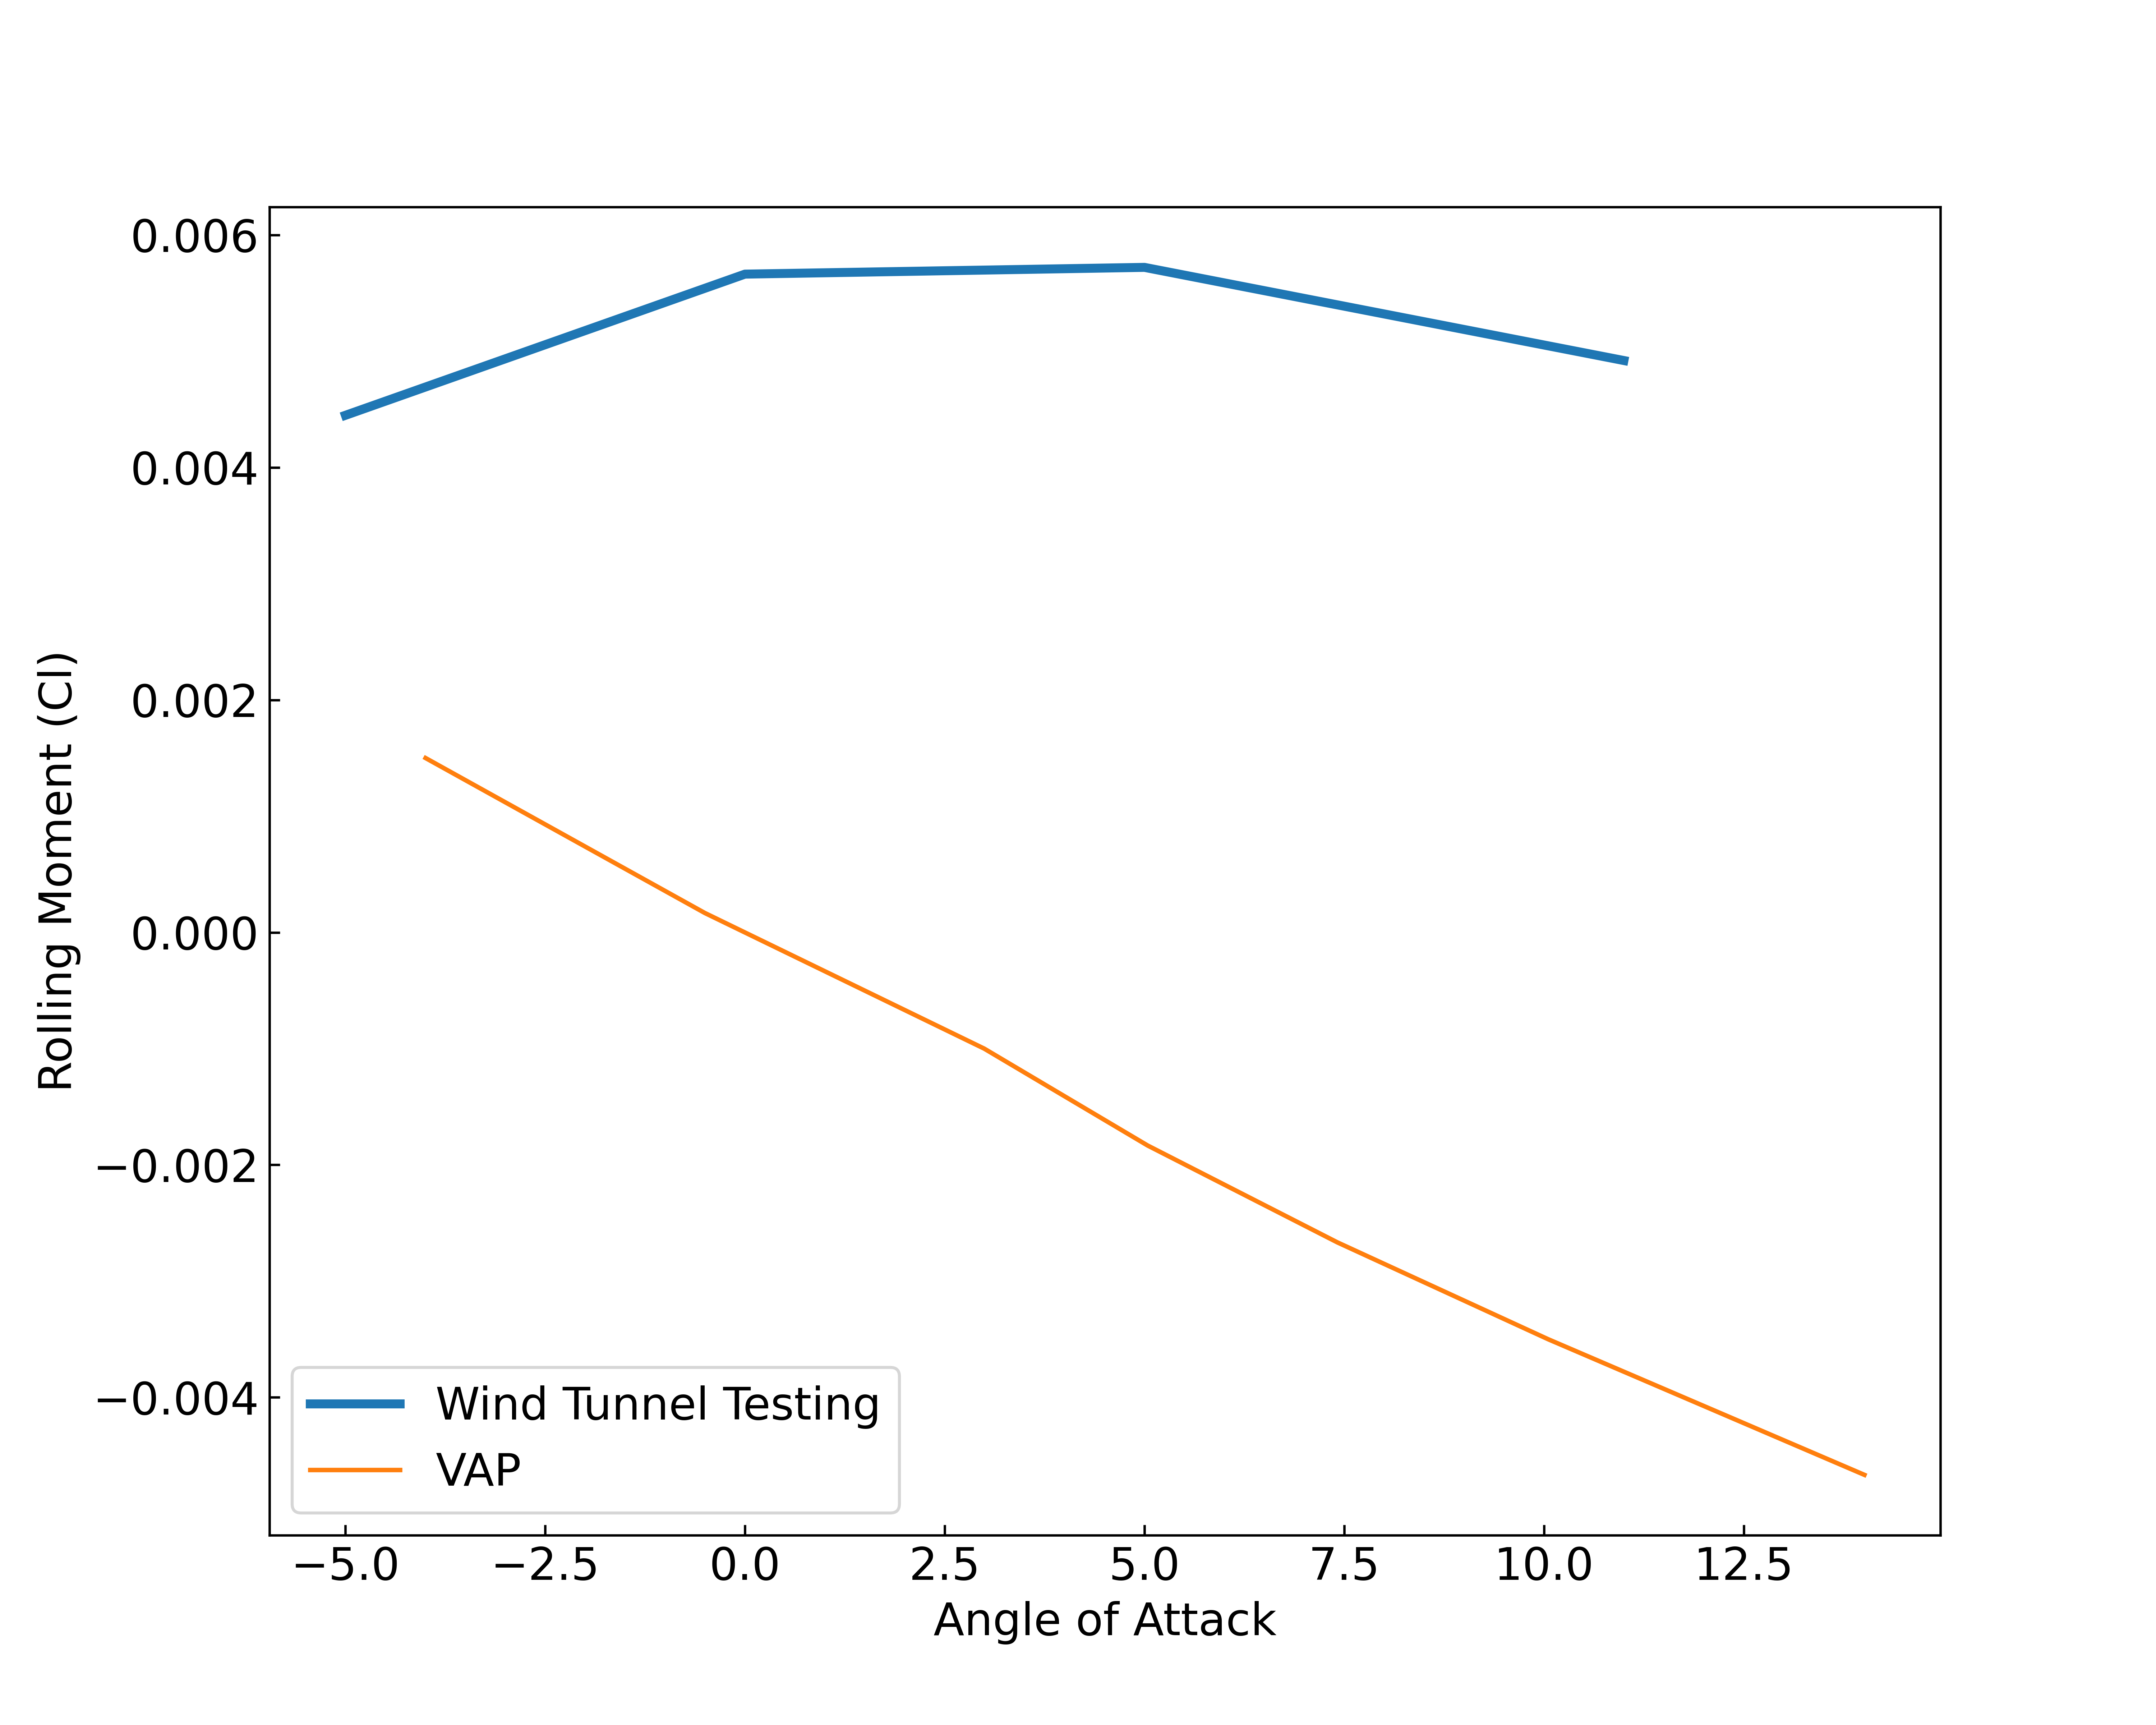
\includegraphics[width=\textwidth]{05_Results/VAP/noProp/Cl/10ms_6000RPM_Cl.png}
        \caption{Rolling Moment Coefficient at 10m/s airspeed and 6000RPM motor speed}
        \label{fig:VAP_NoProp_Cl_10ms_6000}
    \end{subfigure}
    \begin{subfigure}[b]{0.467\textwidth}
        \centering
        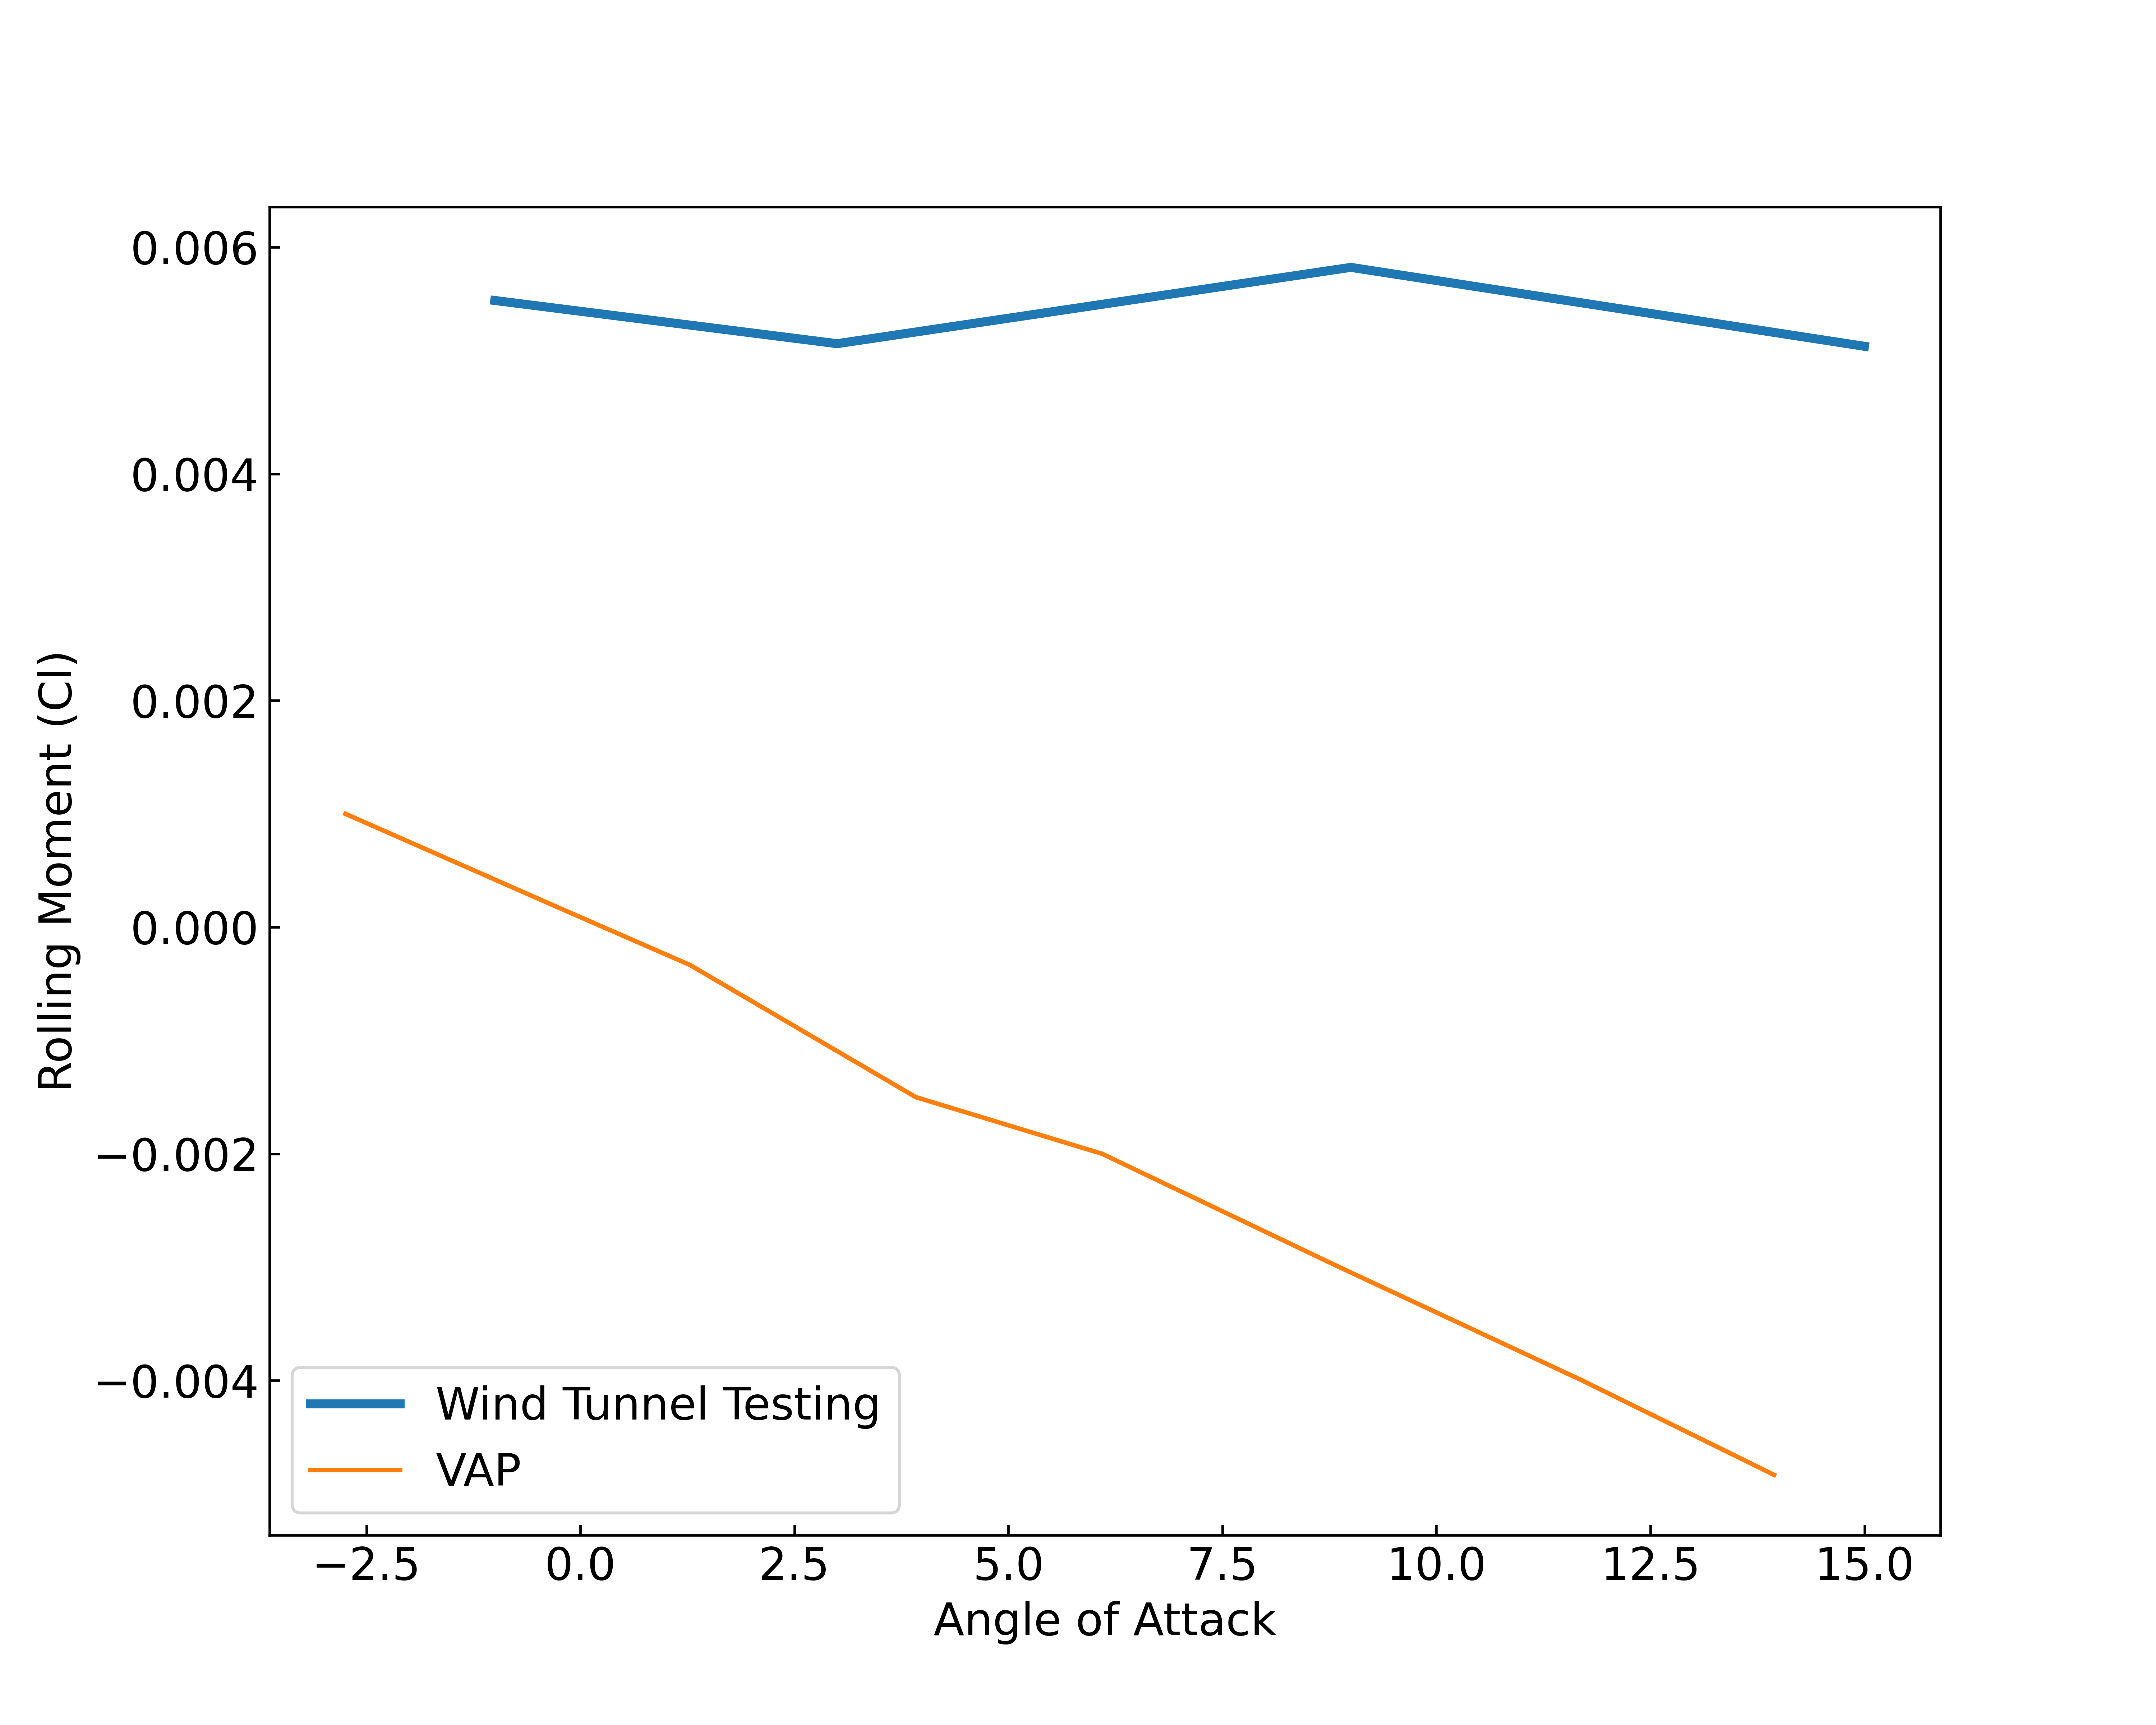
\includegraphics[width=\textwidth]{05_Results/VAP/noProp/Cl/10ms_11000RPM_Cl.png}
        \caption{Rolling Moment Coefficient at 10m/s airspeed and 11000RPM motor speed}
        \label{fig:VAP_NoProp_Cl_10ms_11000}
    \end{subfigure}
    \begin{subfigure}[b]{0.467\textwidth}
        \centering
        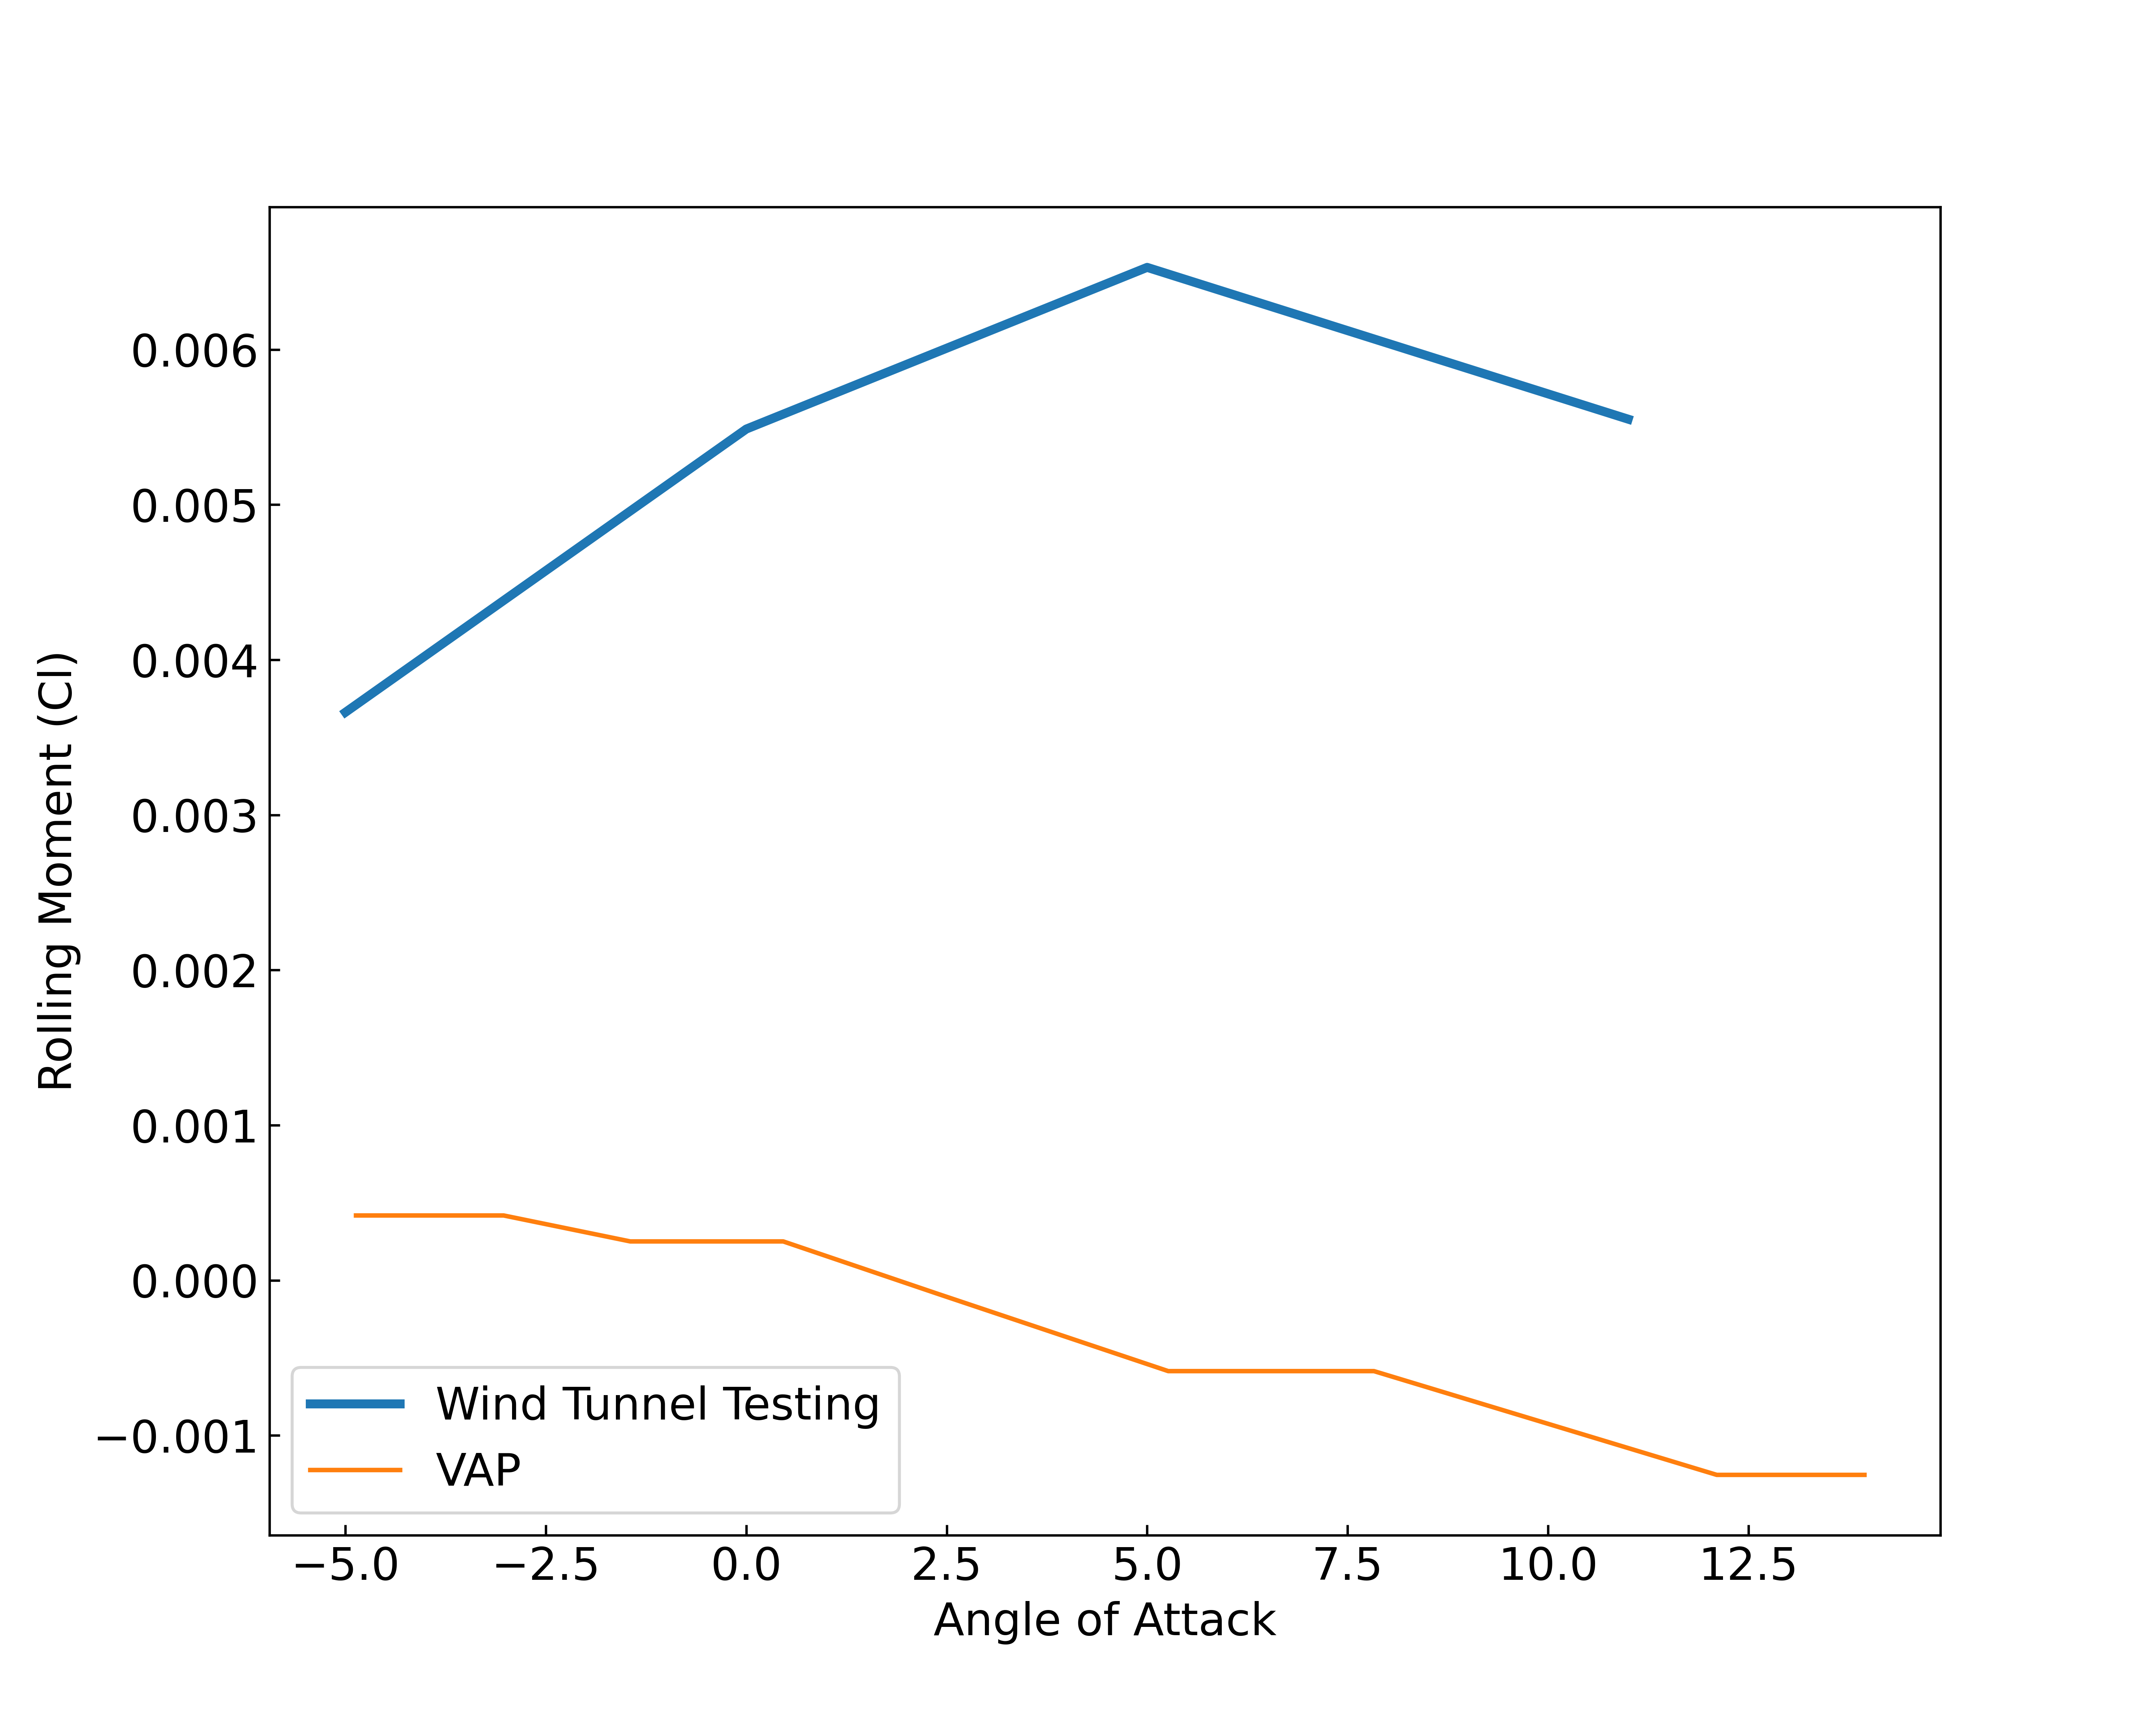
\includegraphics[width=\textwidth]{05_Results/VAP/noProp/Cl/20ms_6000RPM_Cl.png}
        \caption{Rolling Moment Coefficient at 20m/s airspeed and 6000RPM motor speed}
        \label{fig:VAP_NoProp_Cl_20ms_6000}
    \end{subfigure}
    \begin{subfigure}[b]{0.467\textwidth}
        \centering
        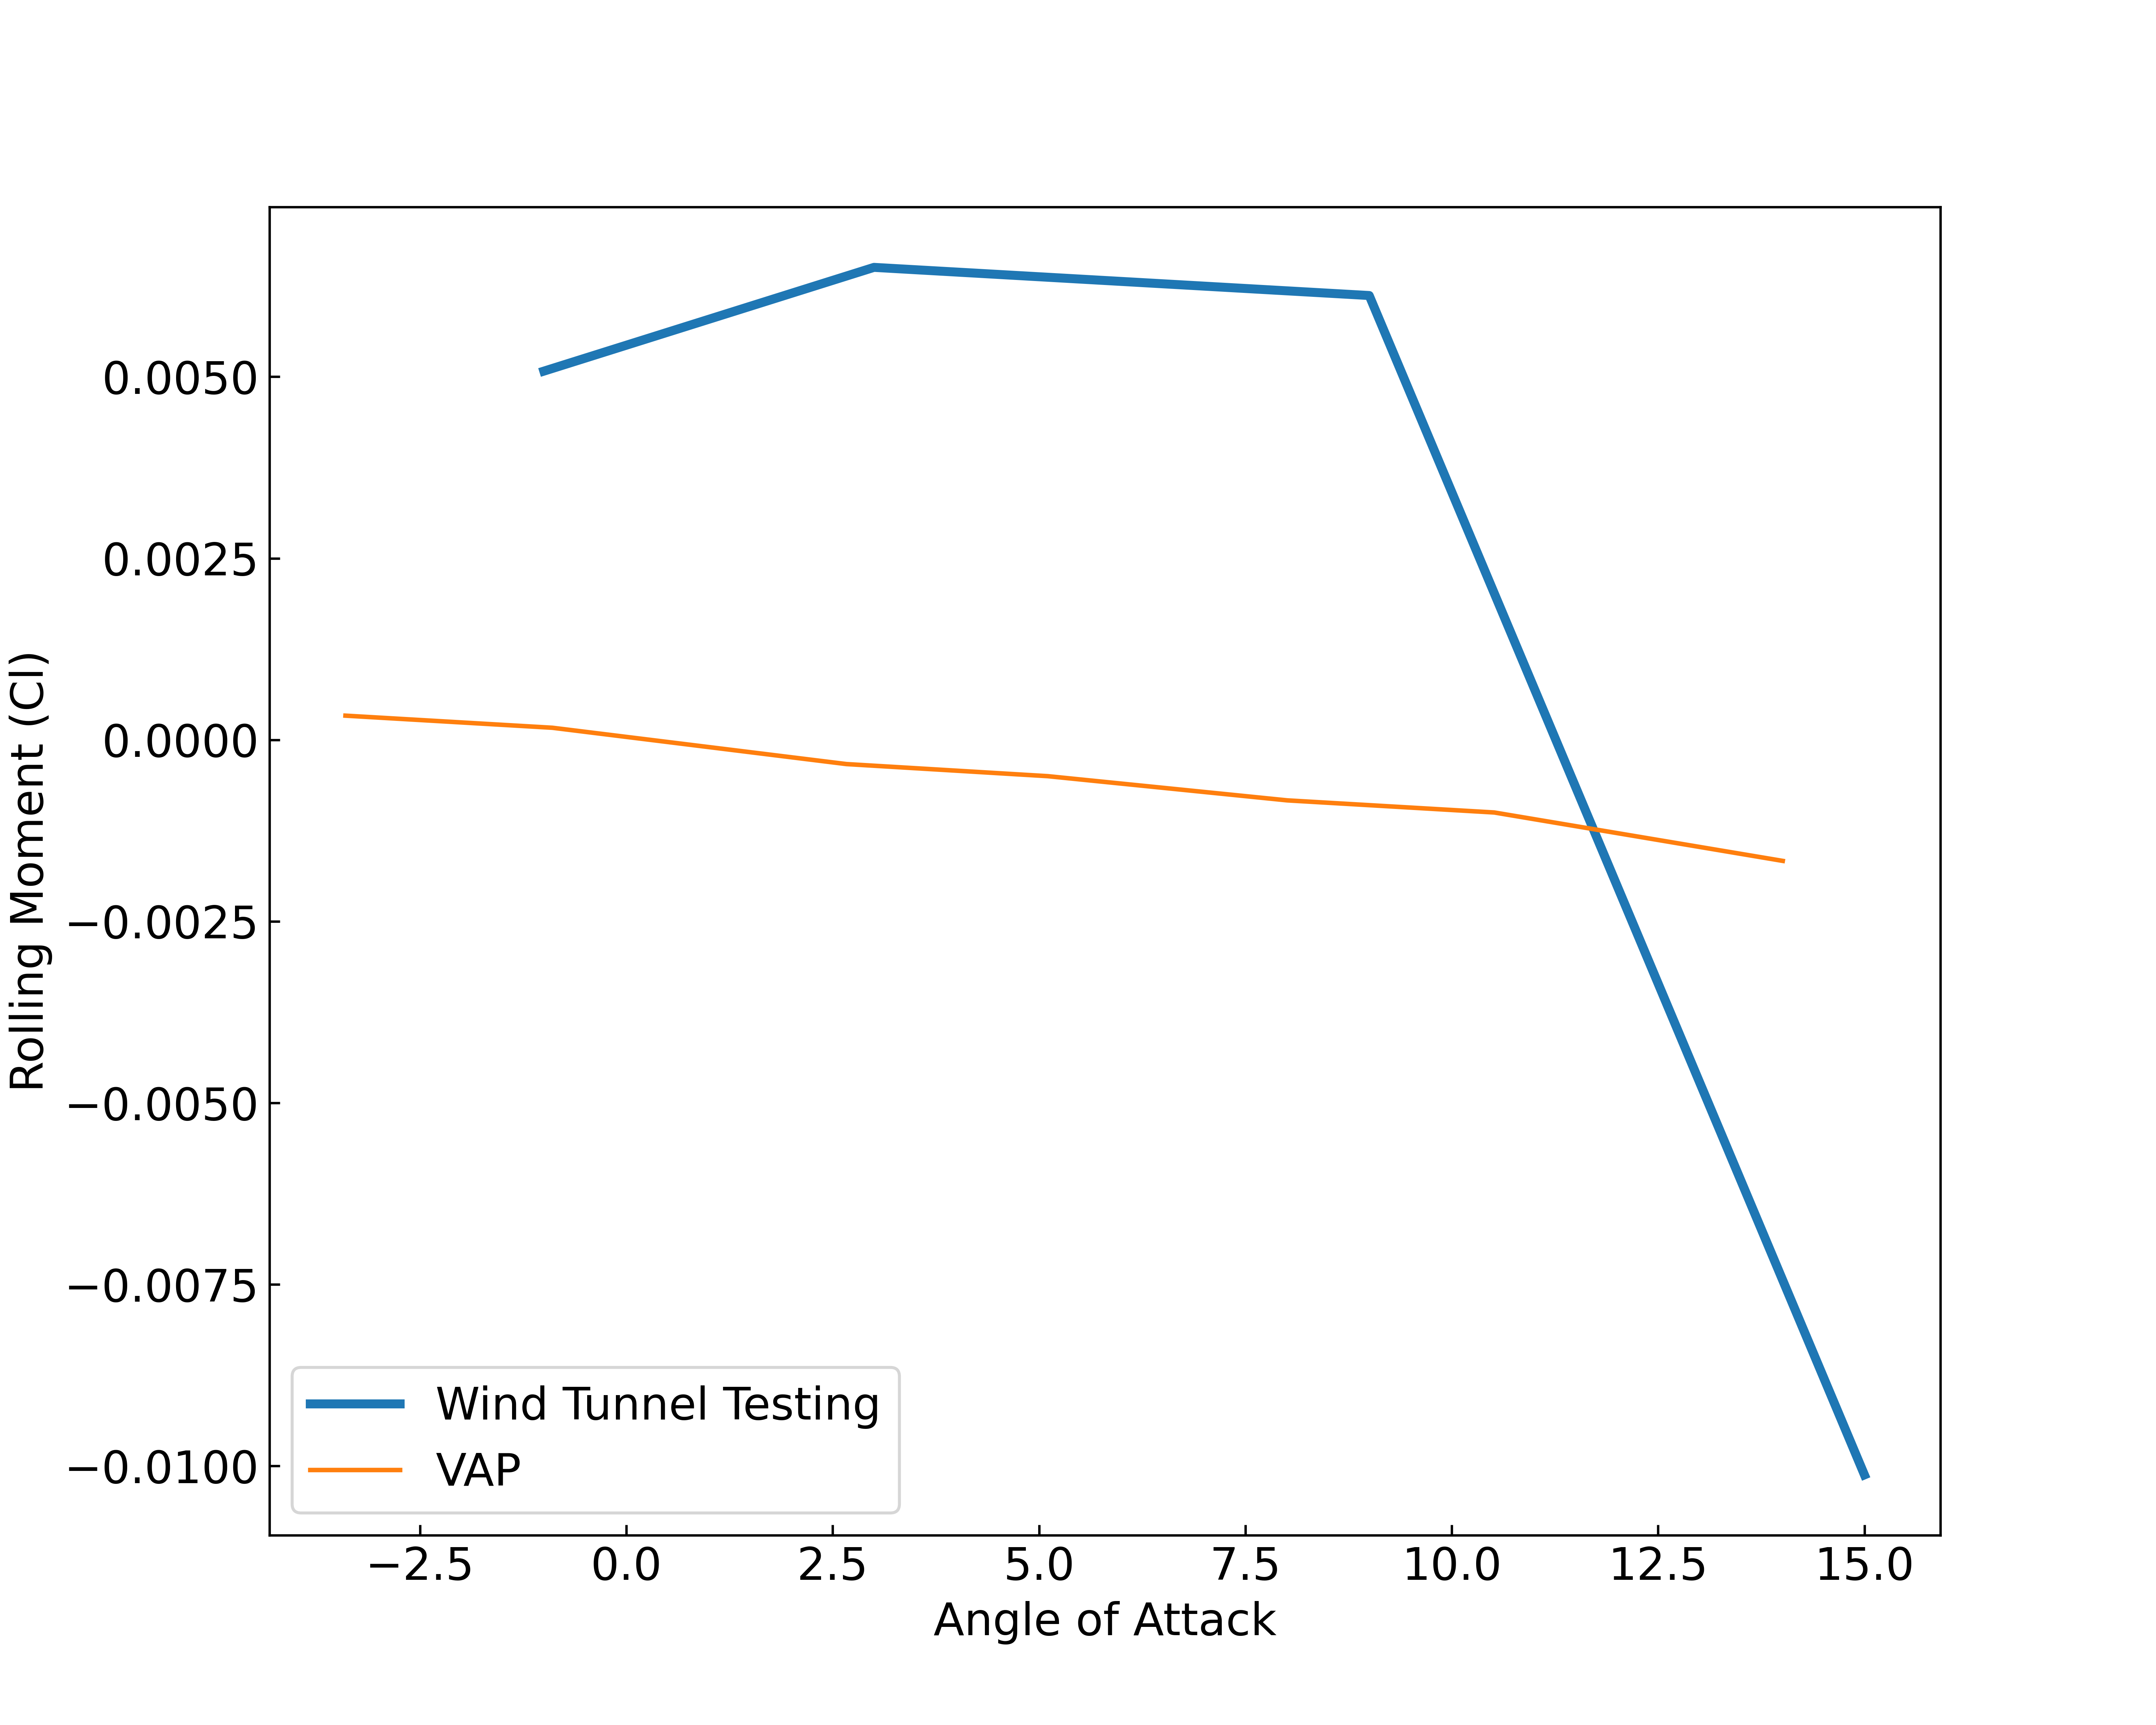
\includegraphics[width=\textwidth]{05_Results/VAP/noProp/Cl/20ms_11000RPM_Cl.png}
        \caption{Rolling Moment Coefficient at 20m/s airspeed and 11000RPM motor speed}
        \label{fig:VAP_NoProp_Cl_20ms_11000}
    \end{subfigure}
\end{figure}


\begin{figure}[H]
    \centering
    \begin{subfigure}[b]{0.467\textwidth}
        \centering
        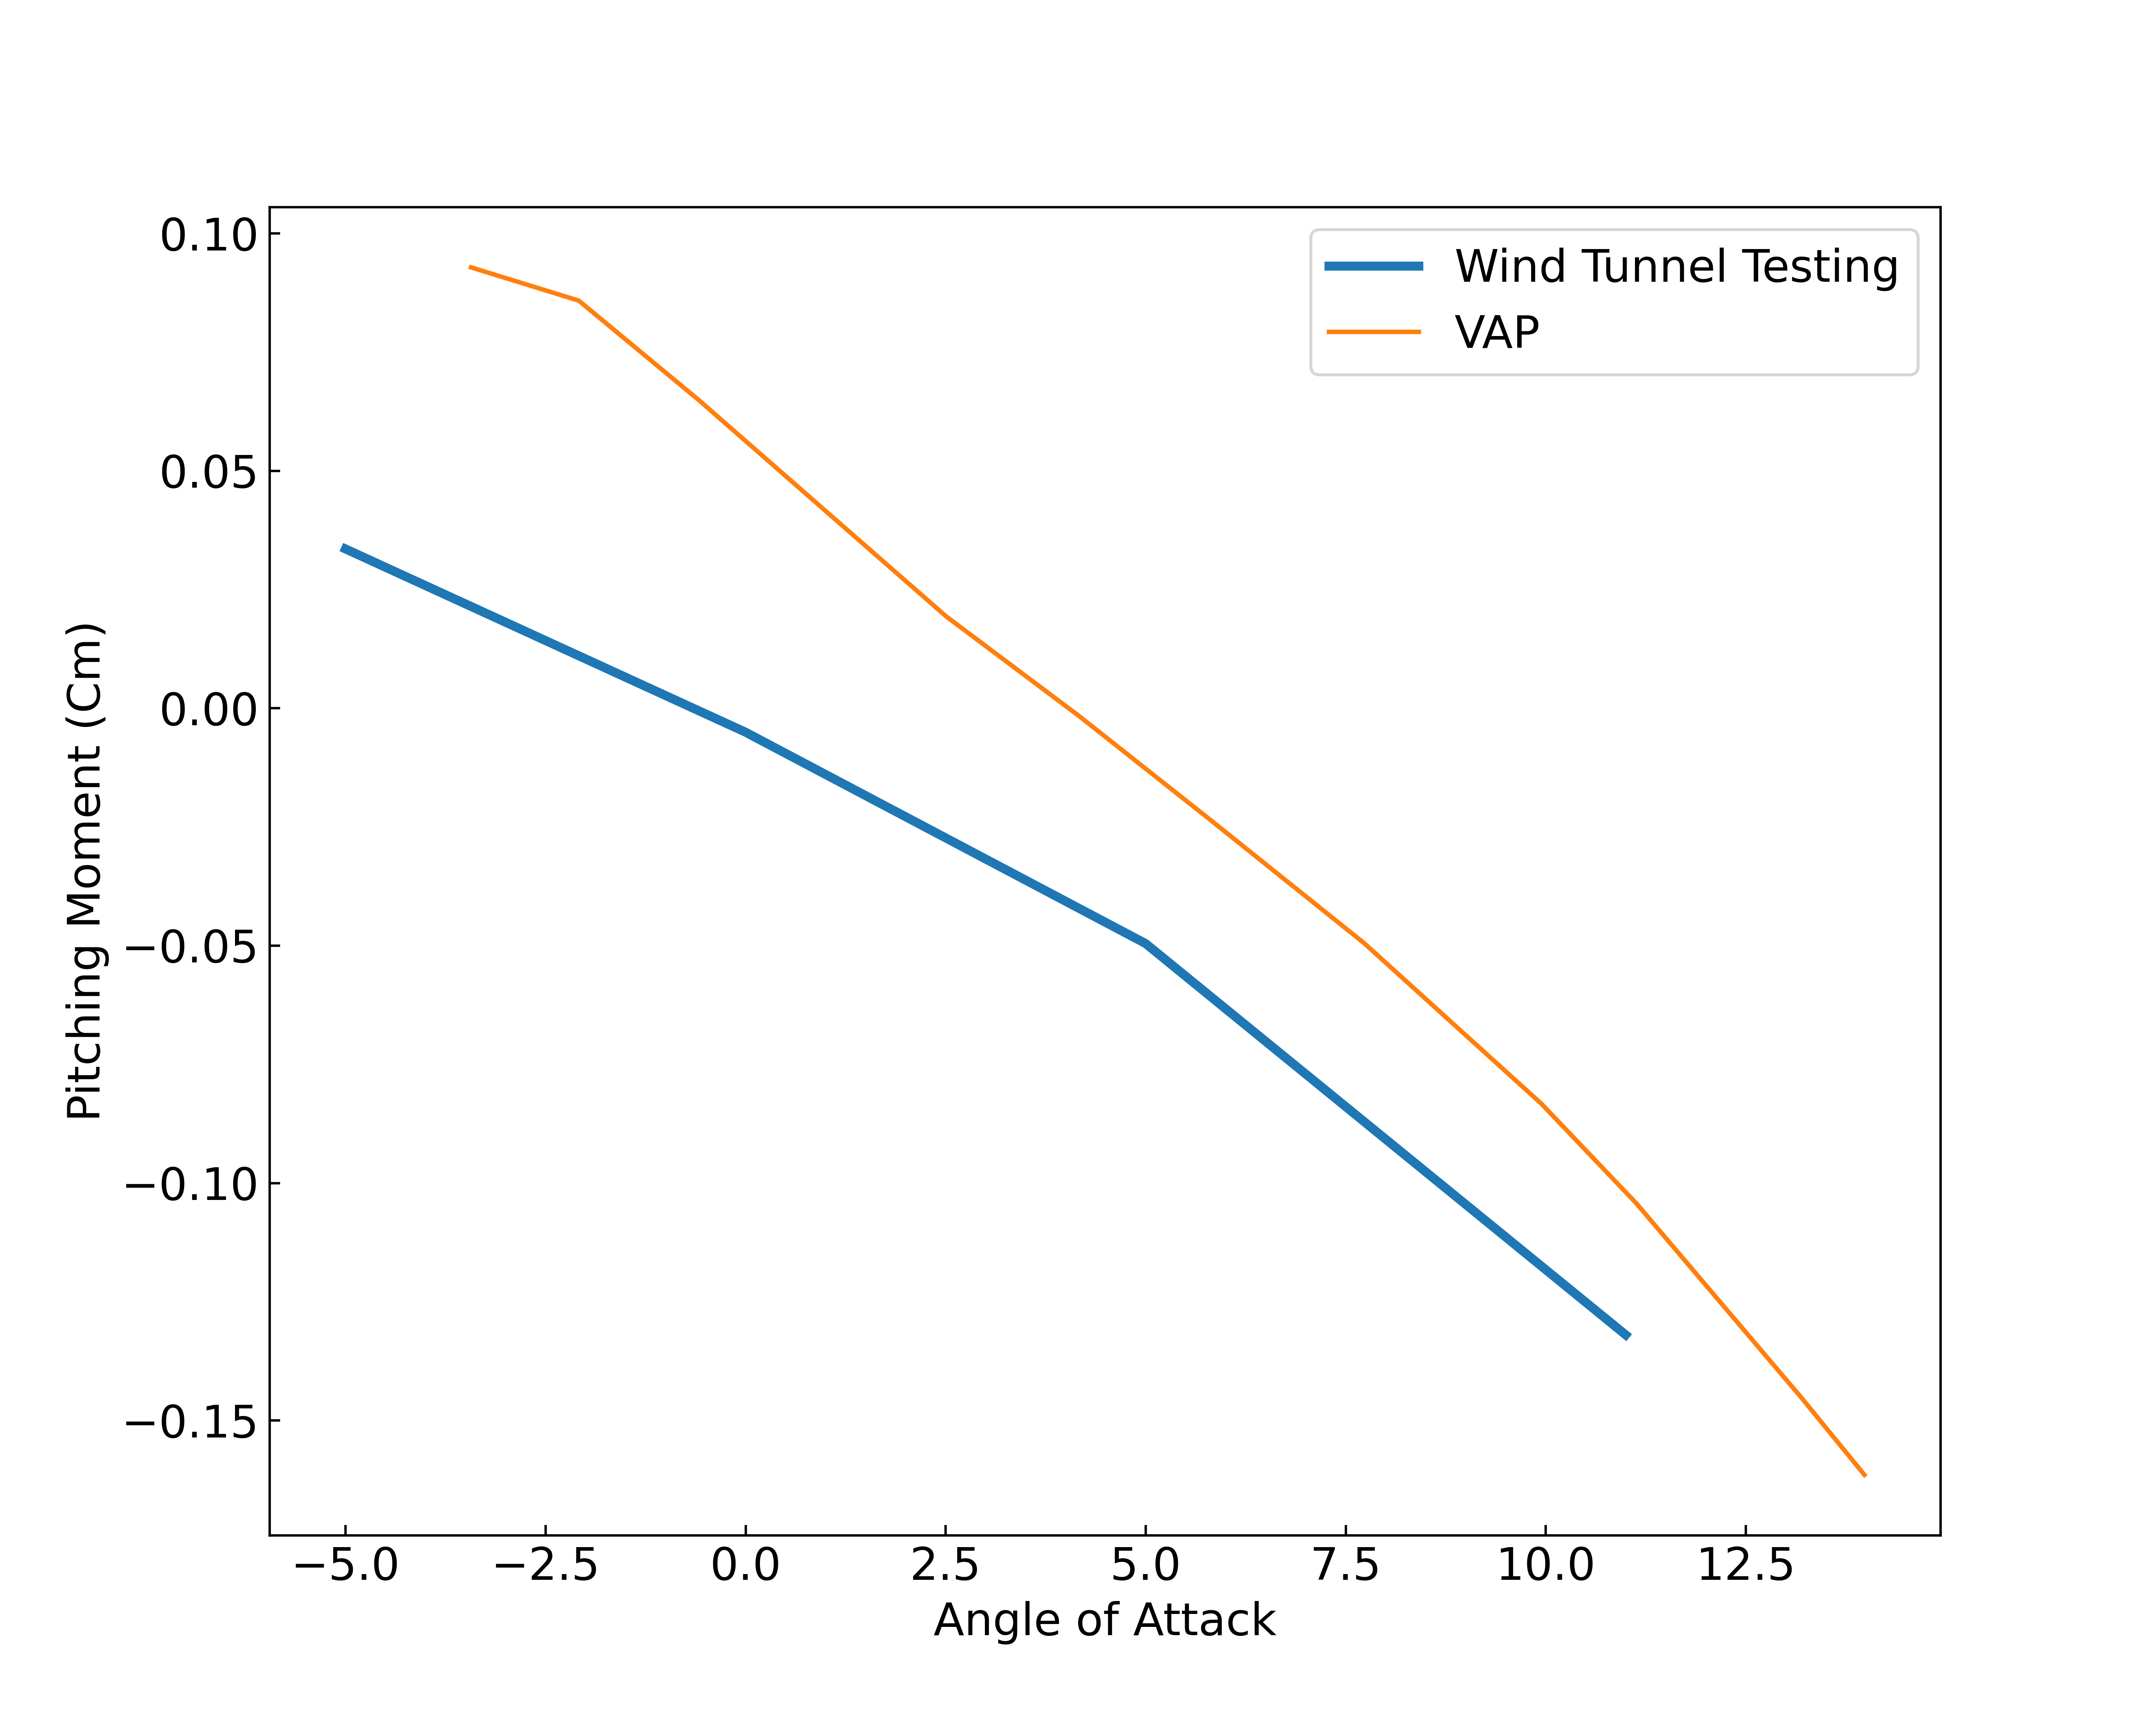
\includegraphics[width=\textwidth]{05_Results/VAP/noProp/Cm/10ms_6000RPM_Cm.png}
        \caption{Pitching Moment Coefficient at 10m/s airspeed and 6000RPM motor speed}
        \label{fig:VAP_NoProp_Cm_10ms_6000}
    \end{subfigure}
    \begin{subfigure}[b]{0.467\textwidth}
        \centering
        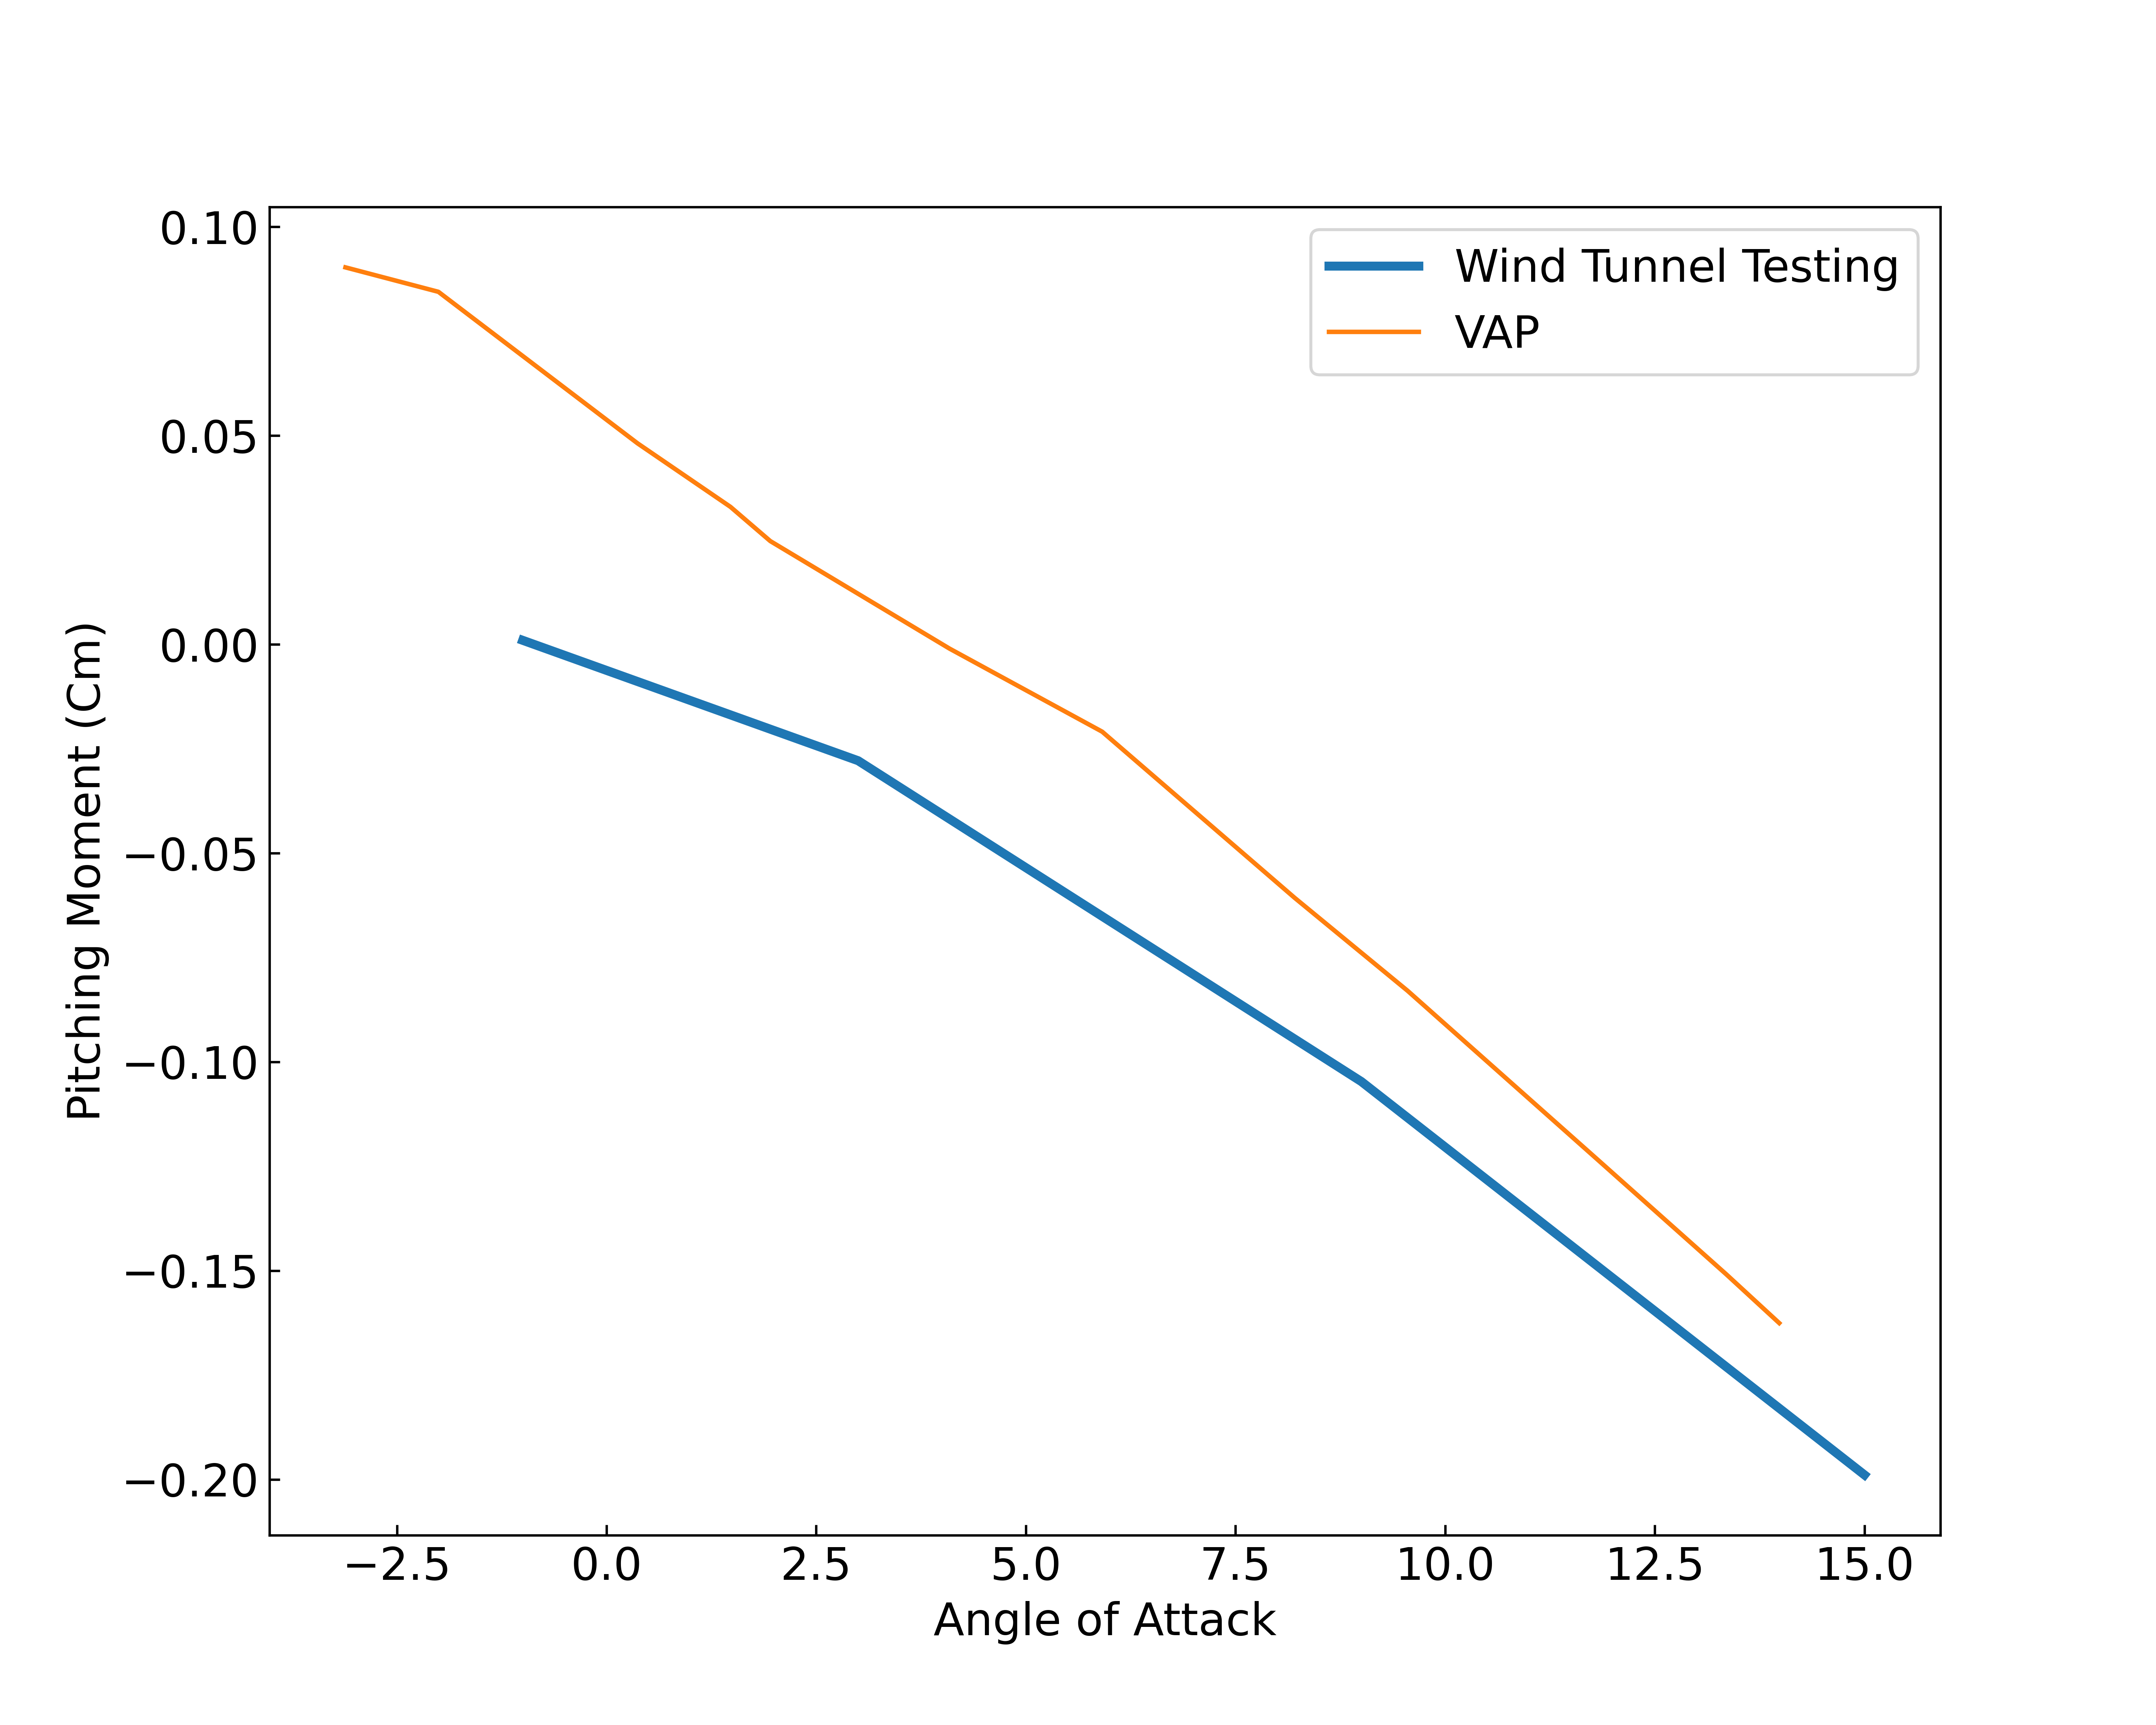
\includegraphics[width=\textwidth]{05_Results/VAP/noProp/Cm/10ms_11000RPM_Cm.png}
        \caption{Pitching Moment Coefficient at 10m/s airspeed and 11000RPM motor speed}
        \label{fig:VAP_NoProp_Cm_10ms_11000}
    \end{subfigure}
    \begin{subfigure}[b]{0.467\textwidth}
        \centering
        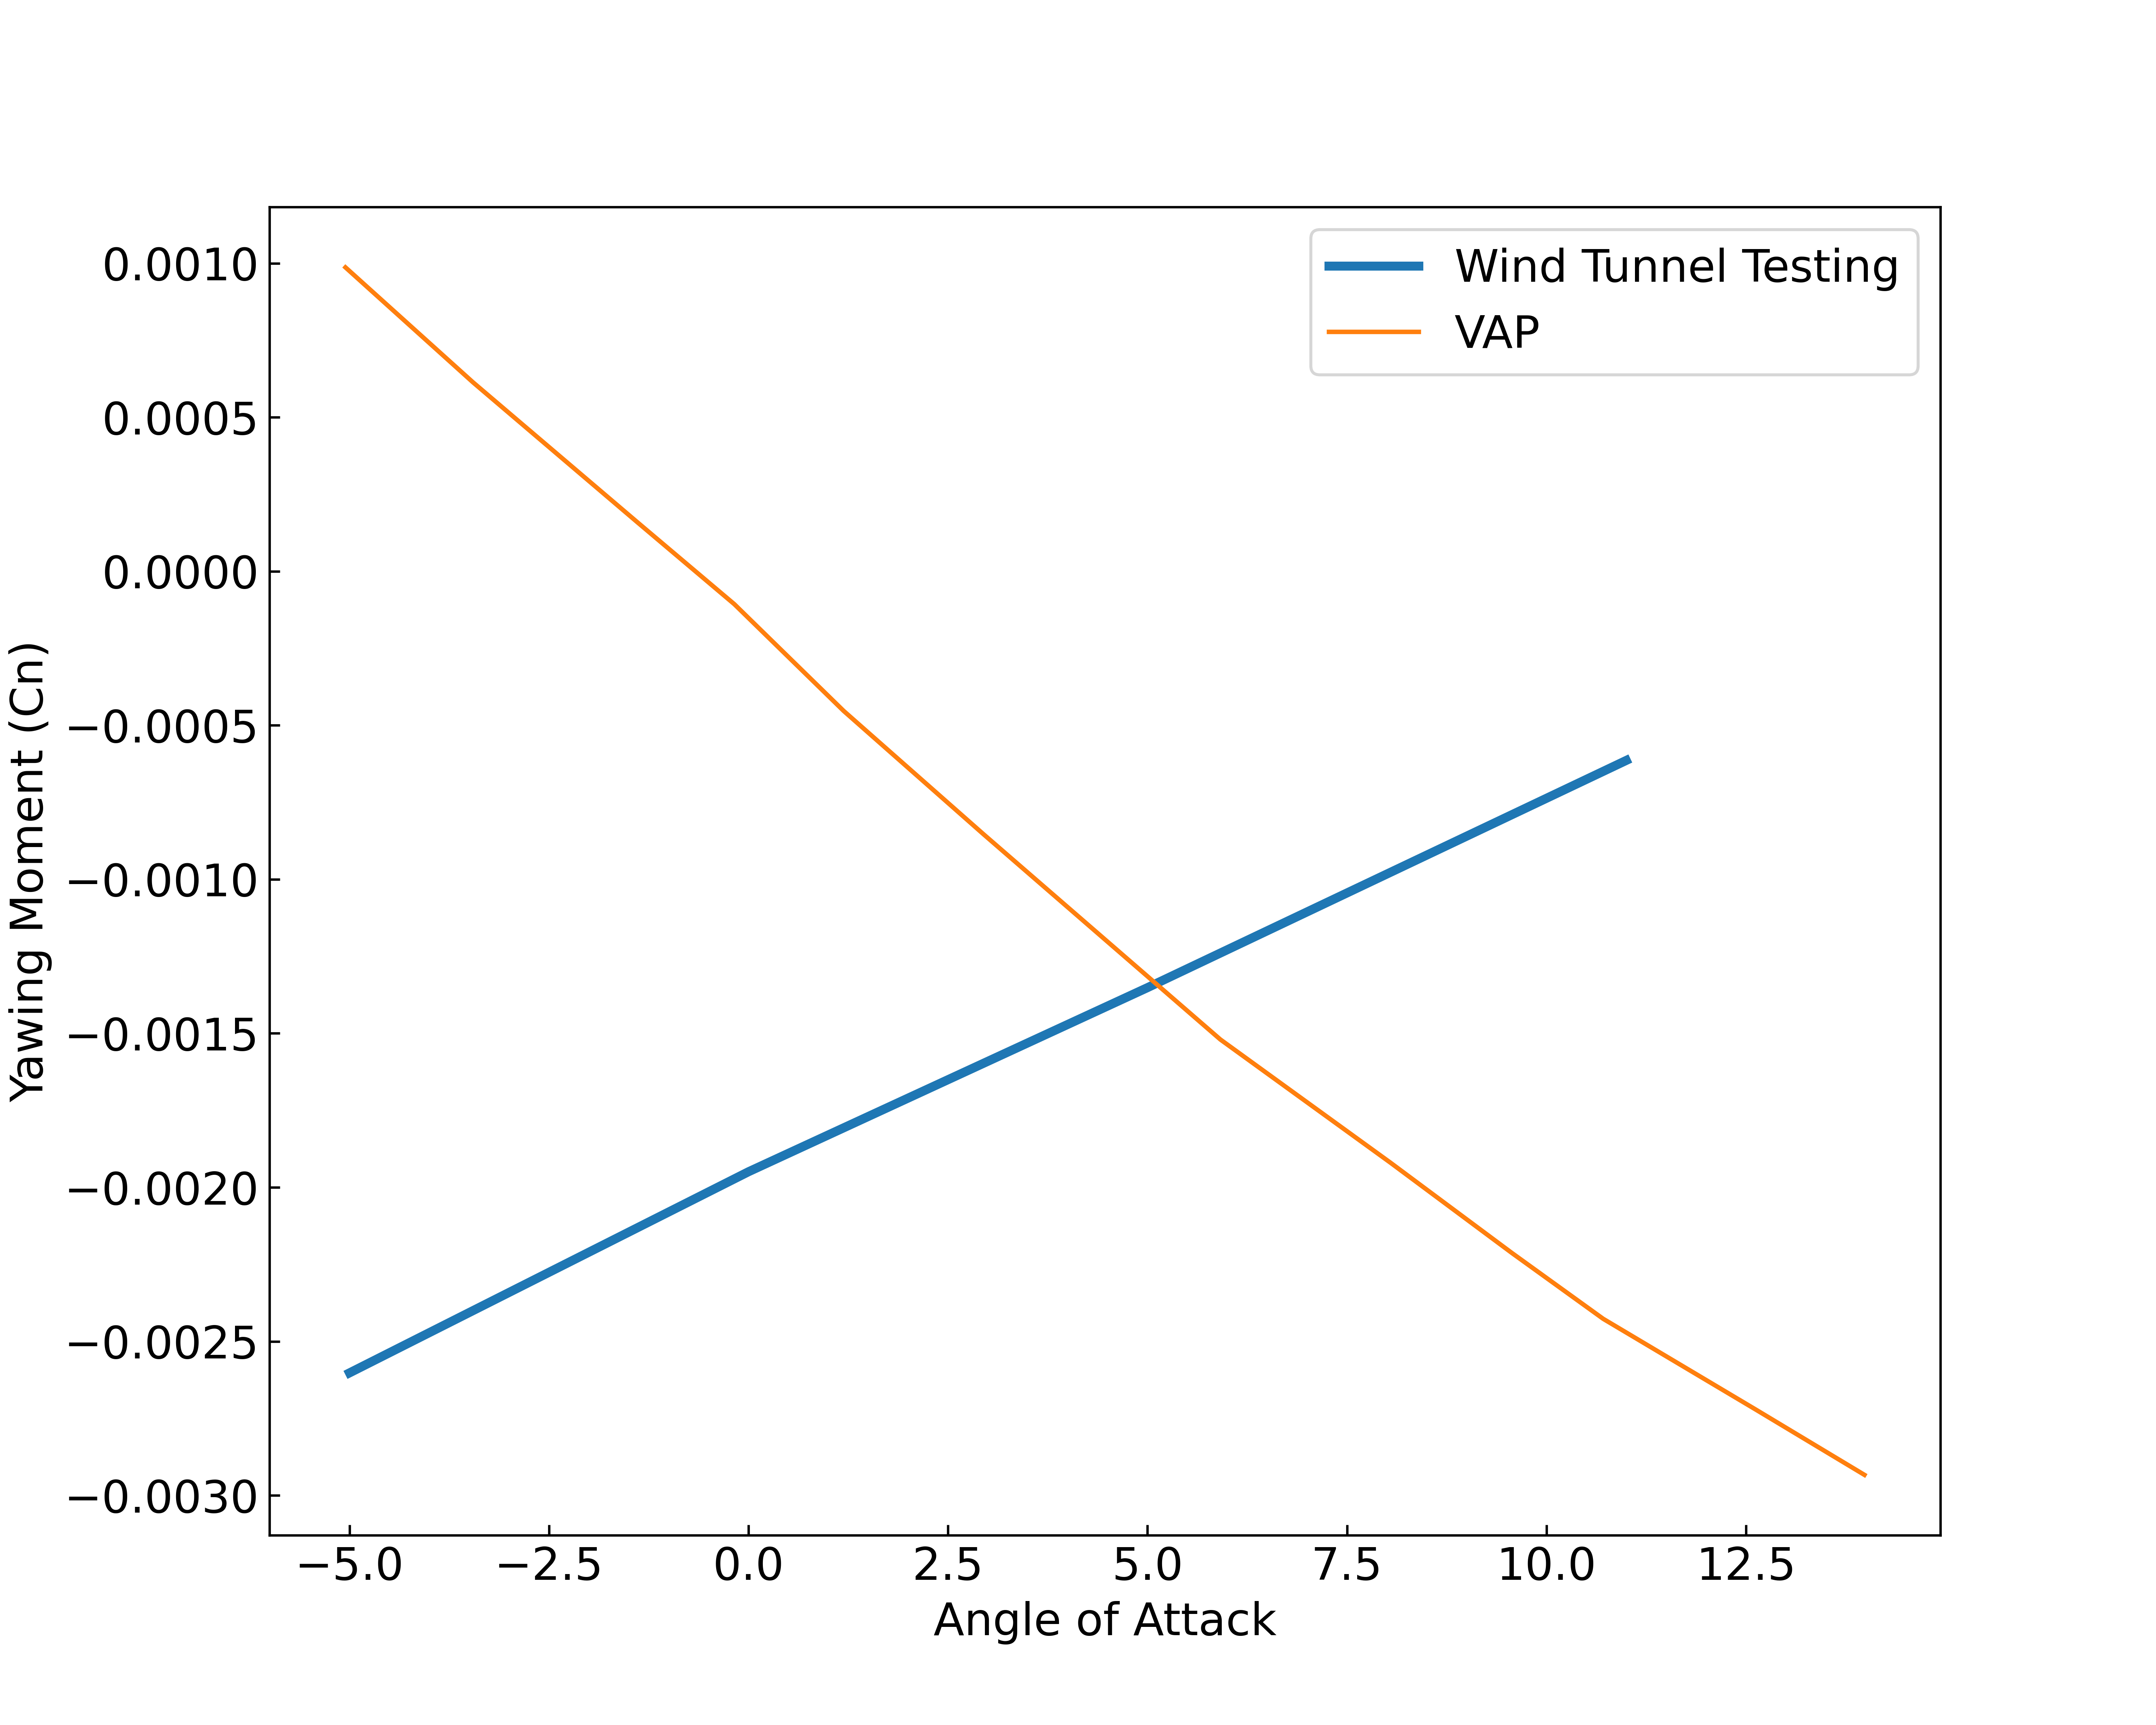
\includegraphics[width=\textwidth]{05_Results/VAP/noProp/Cn/20ms_6000RPM_Cn.png}
        \caption{Pitching Moment Coefficient at 20m/s airspeed and 6000RPM motor speed}
        \label{fig:VAP_NoProp_Cm_20ms_6000}
    \end{subfigure}
    \begin{subfigure}[b]{0.467\textwidth}
        \centering
        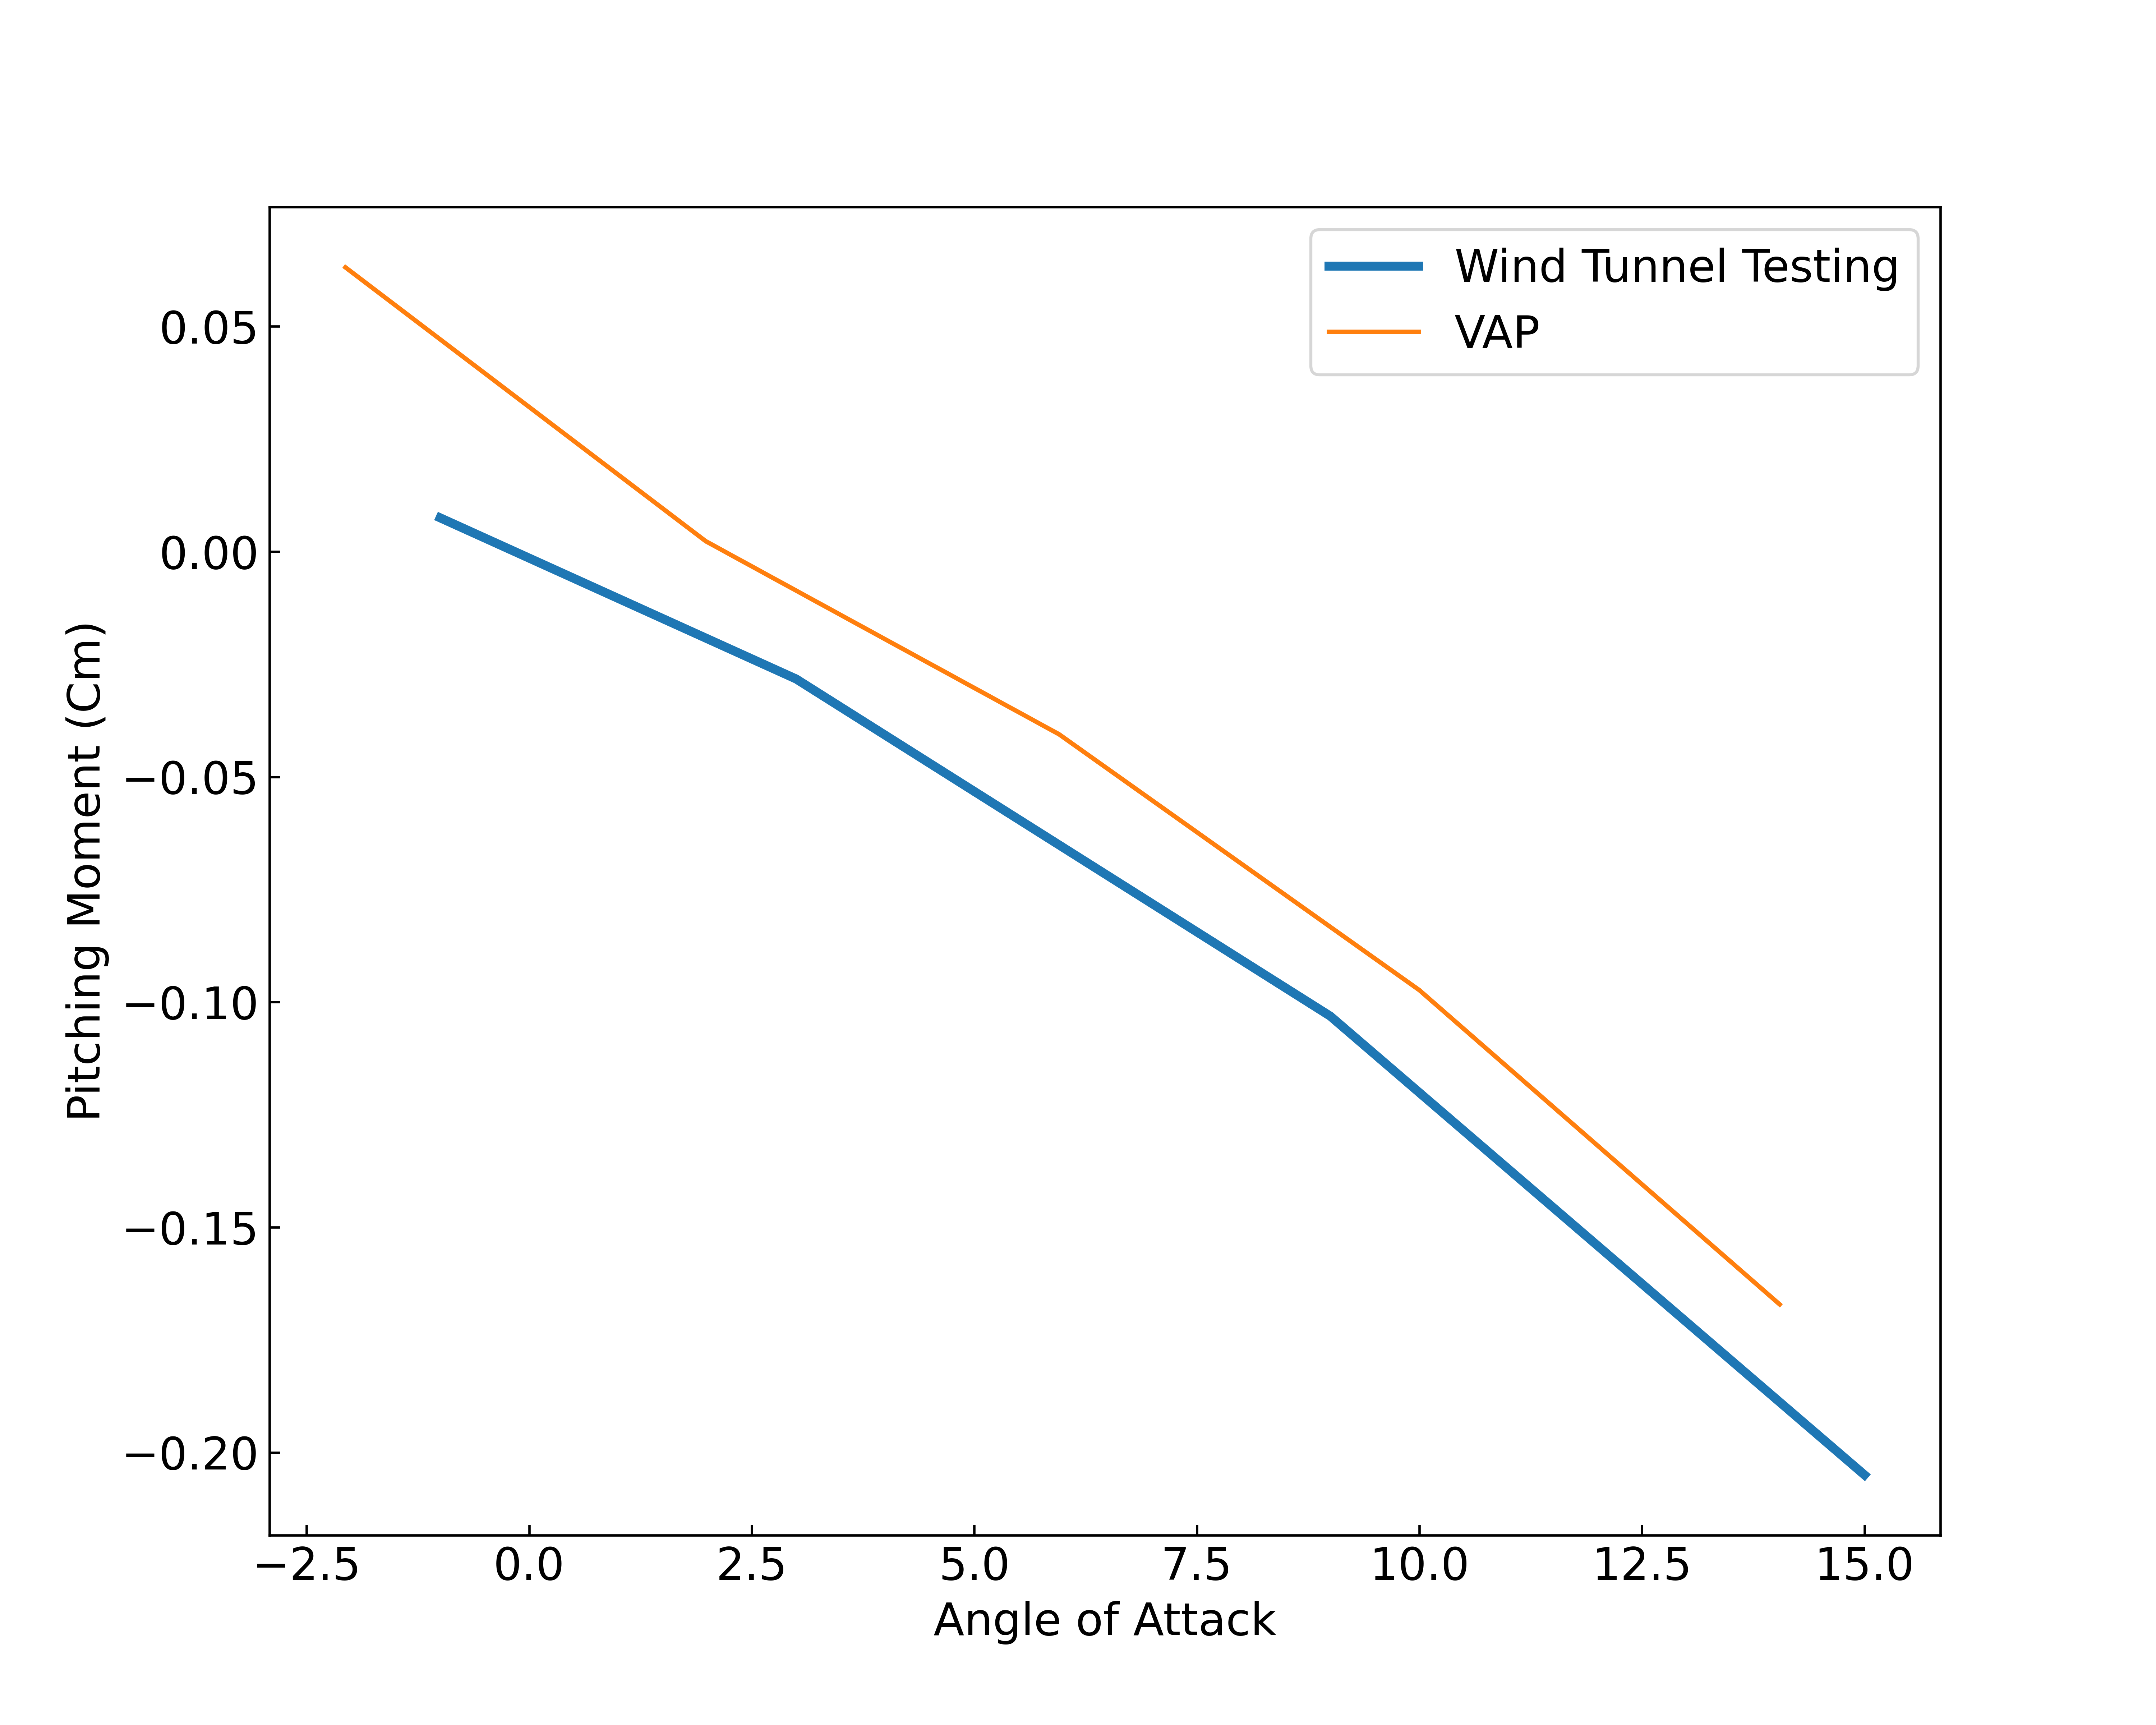
\includegraphics[width=\textwidth]{05_Results/VAP/noProp/Cm/20ms_11000RPM_Cm.png}
        \caption{Pitching Moment Coefficient at 20m/s airspeed and 11000RPM motor speed}
        \label{fig:VAP_NoProp_Cm_20ms_11000}
    \end{subfigure}
\end{figure}



\begin{figure}[H]
    \centering
    \begin{subfigure}[b]{0.467\textwidth}
        \centering
        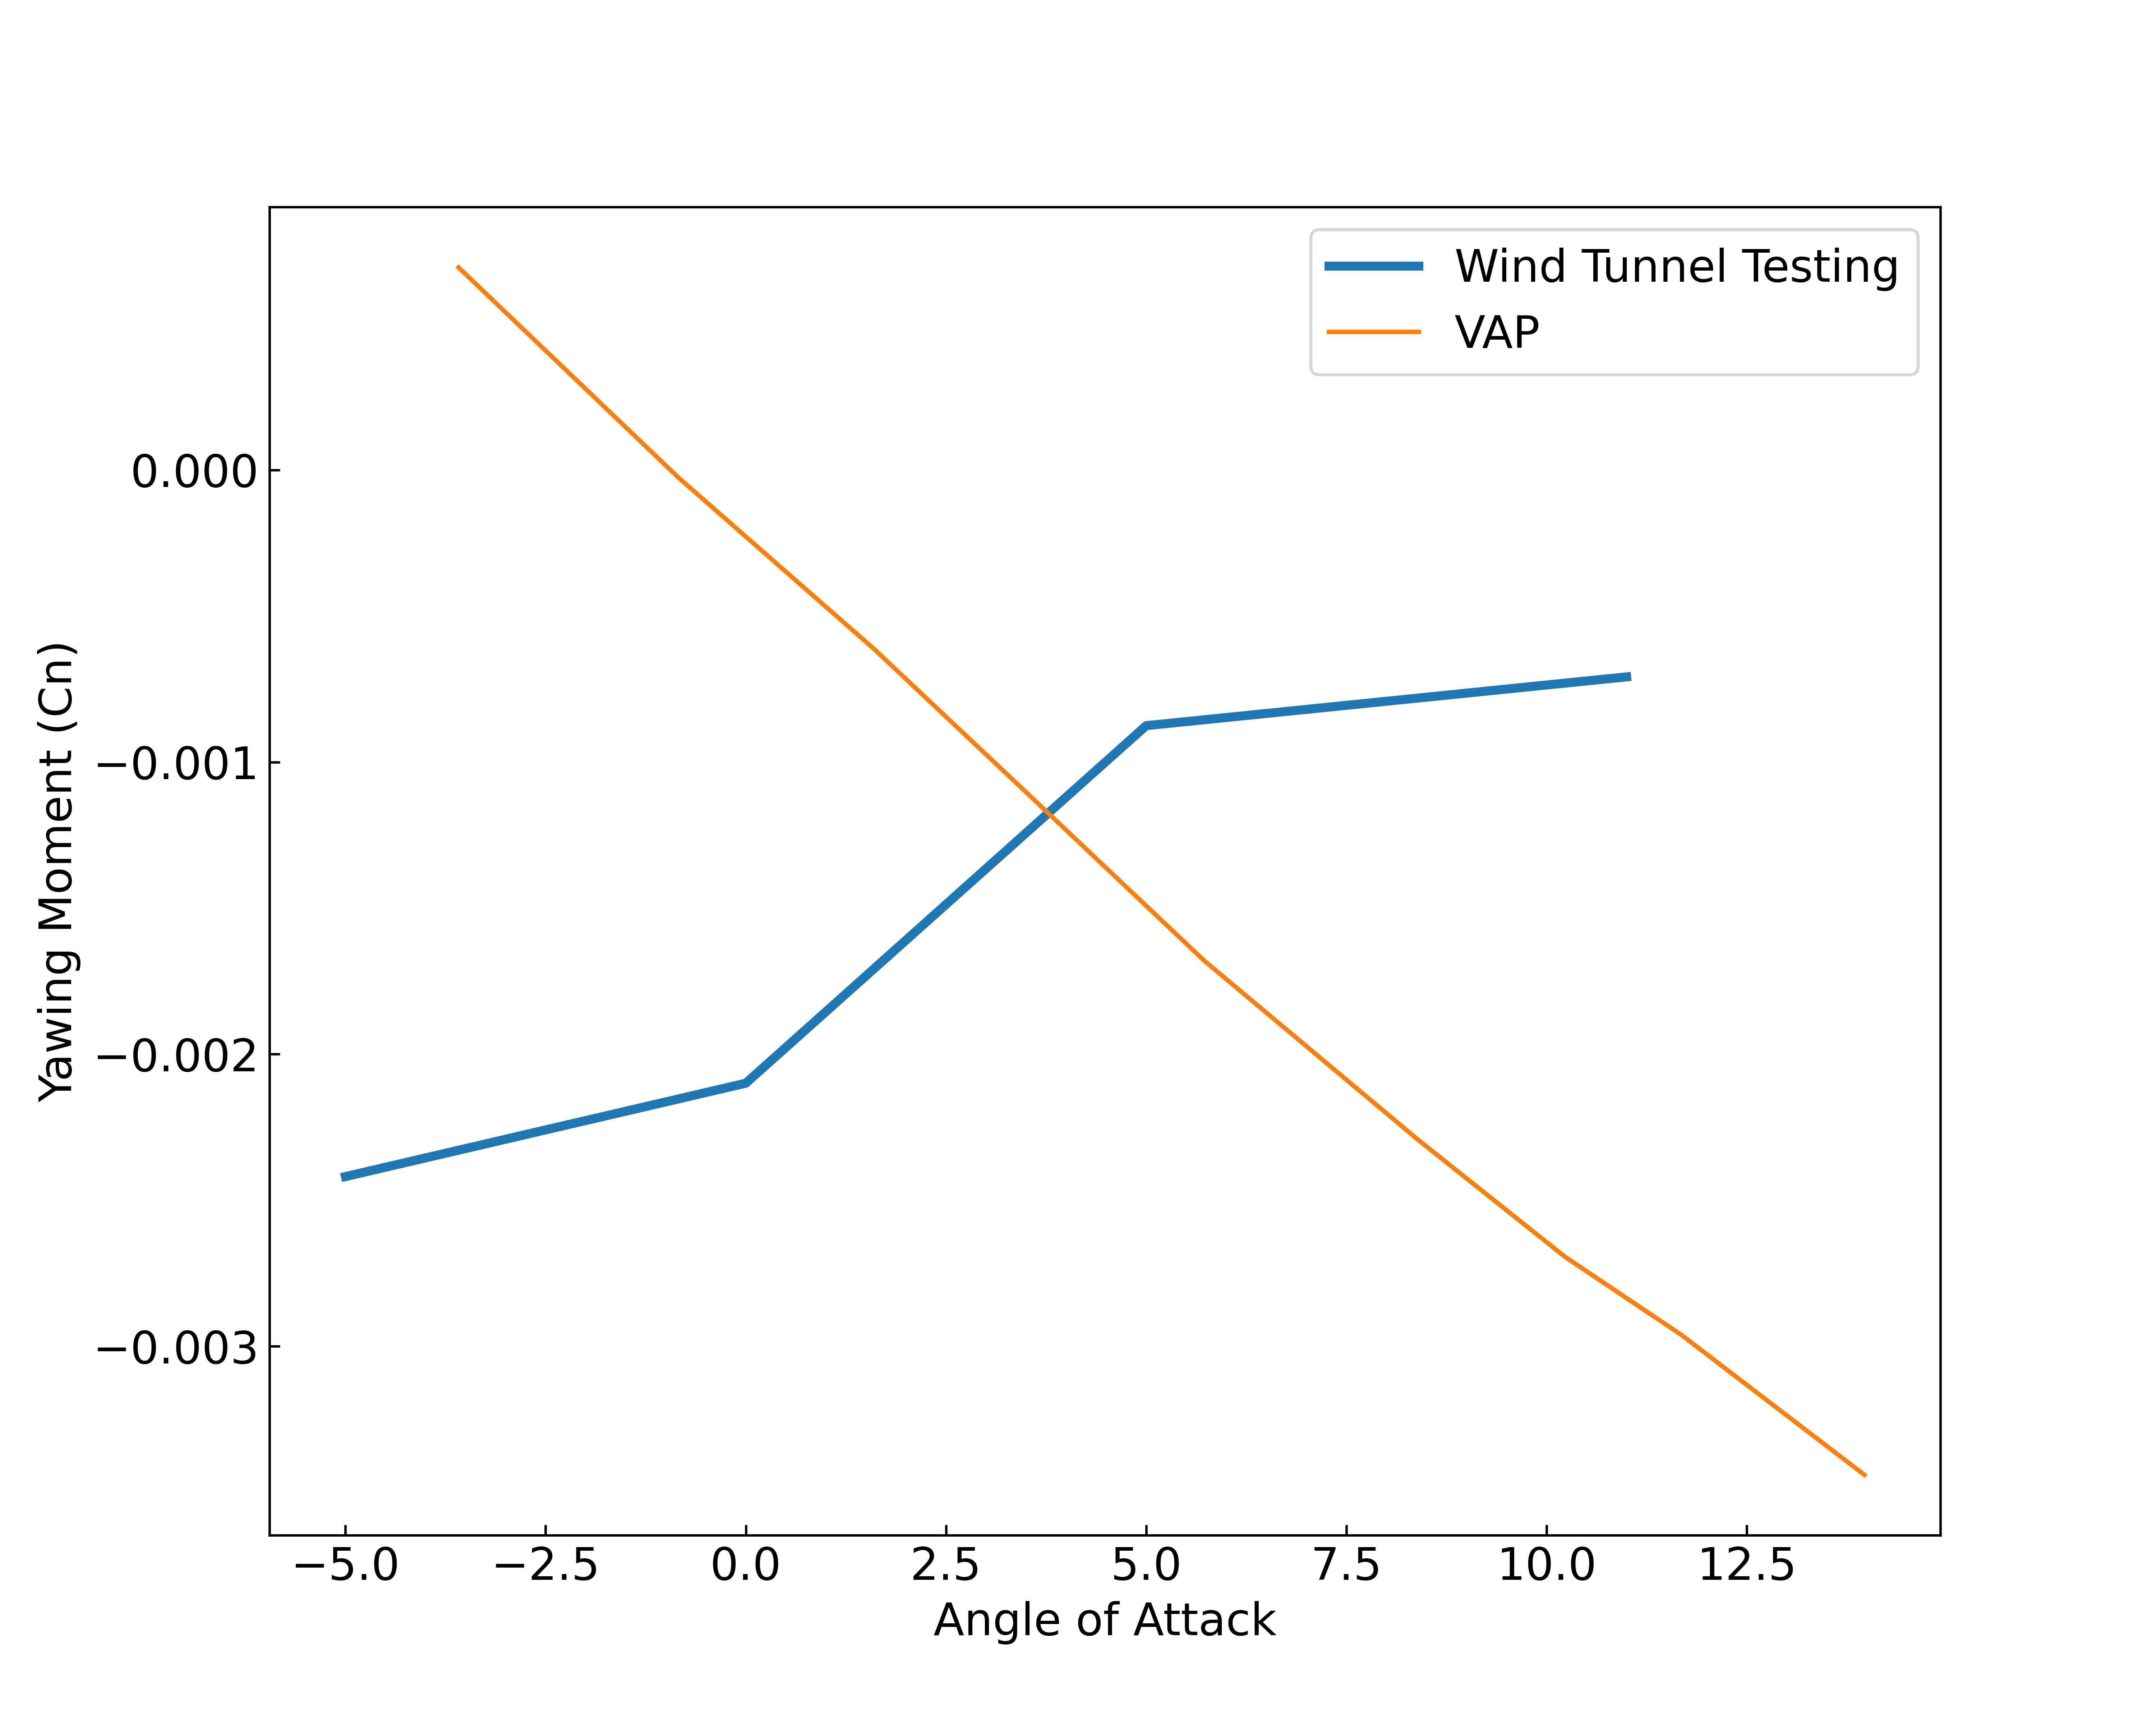
\includegraphics[width=\textwidth]{05_Results/VAP/noProp/Cn/10ms_6000RPM_Cn.png}
        \caption{Yawing Moment Coefficient at 10m/s airspeed and 6000RPM motor speed}
        \label{fig:VAP_noProp_Cm_10ms_6000}
    \end{subfigure}
    \begin{subfigure}[b]{0.467\textwidth}
        \centering
        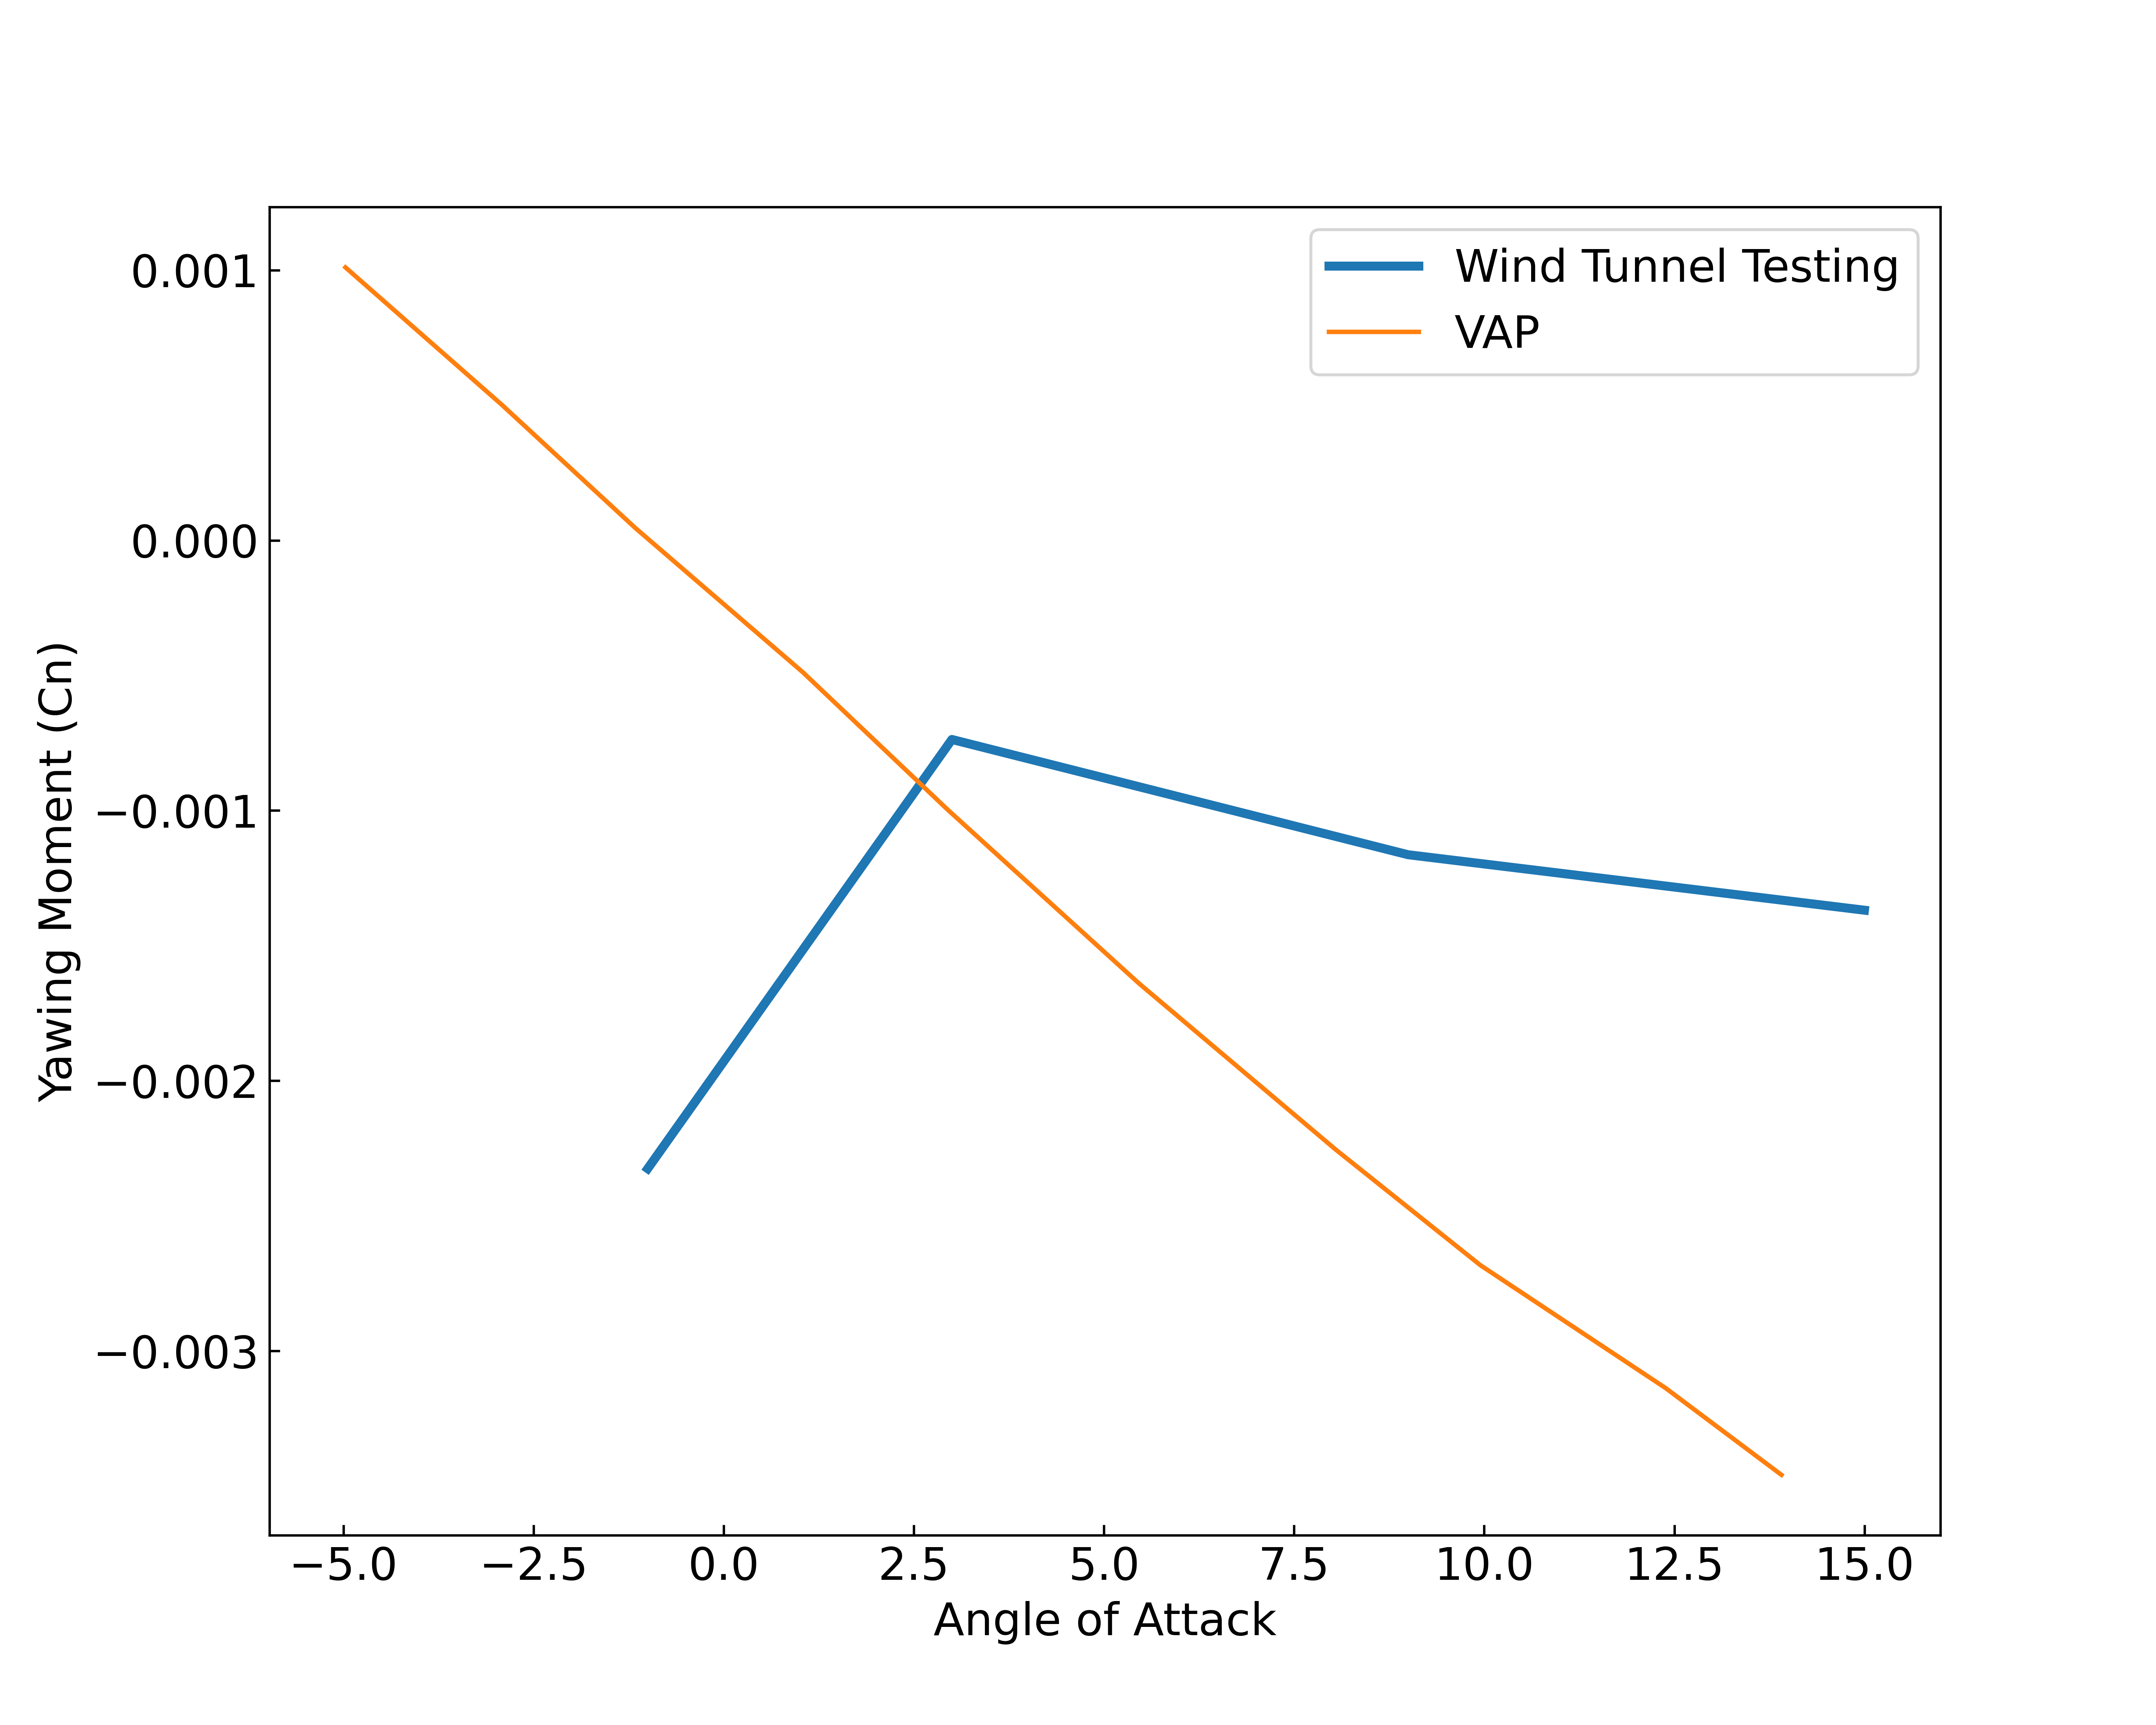
\includegraphics[width=\textwidth]{05_Results/VAP/noProp/Cn/10ms_11000RPM_Cn.png}
        \caption{Yawing Moment Coefficient at 10m/s airspeed and 11000RPM motor speed}
        \label{fig:VAP_noProp_Cm_10ms_11000}
    \end{subfigure}
    \begin{subfigure}[b]{0.467\textwidth}
        \centering
        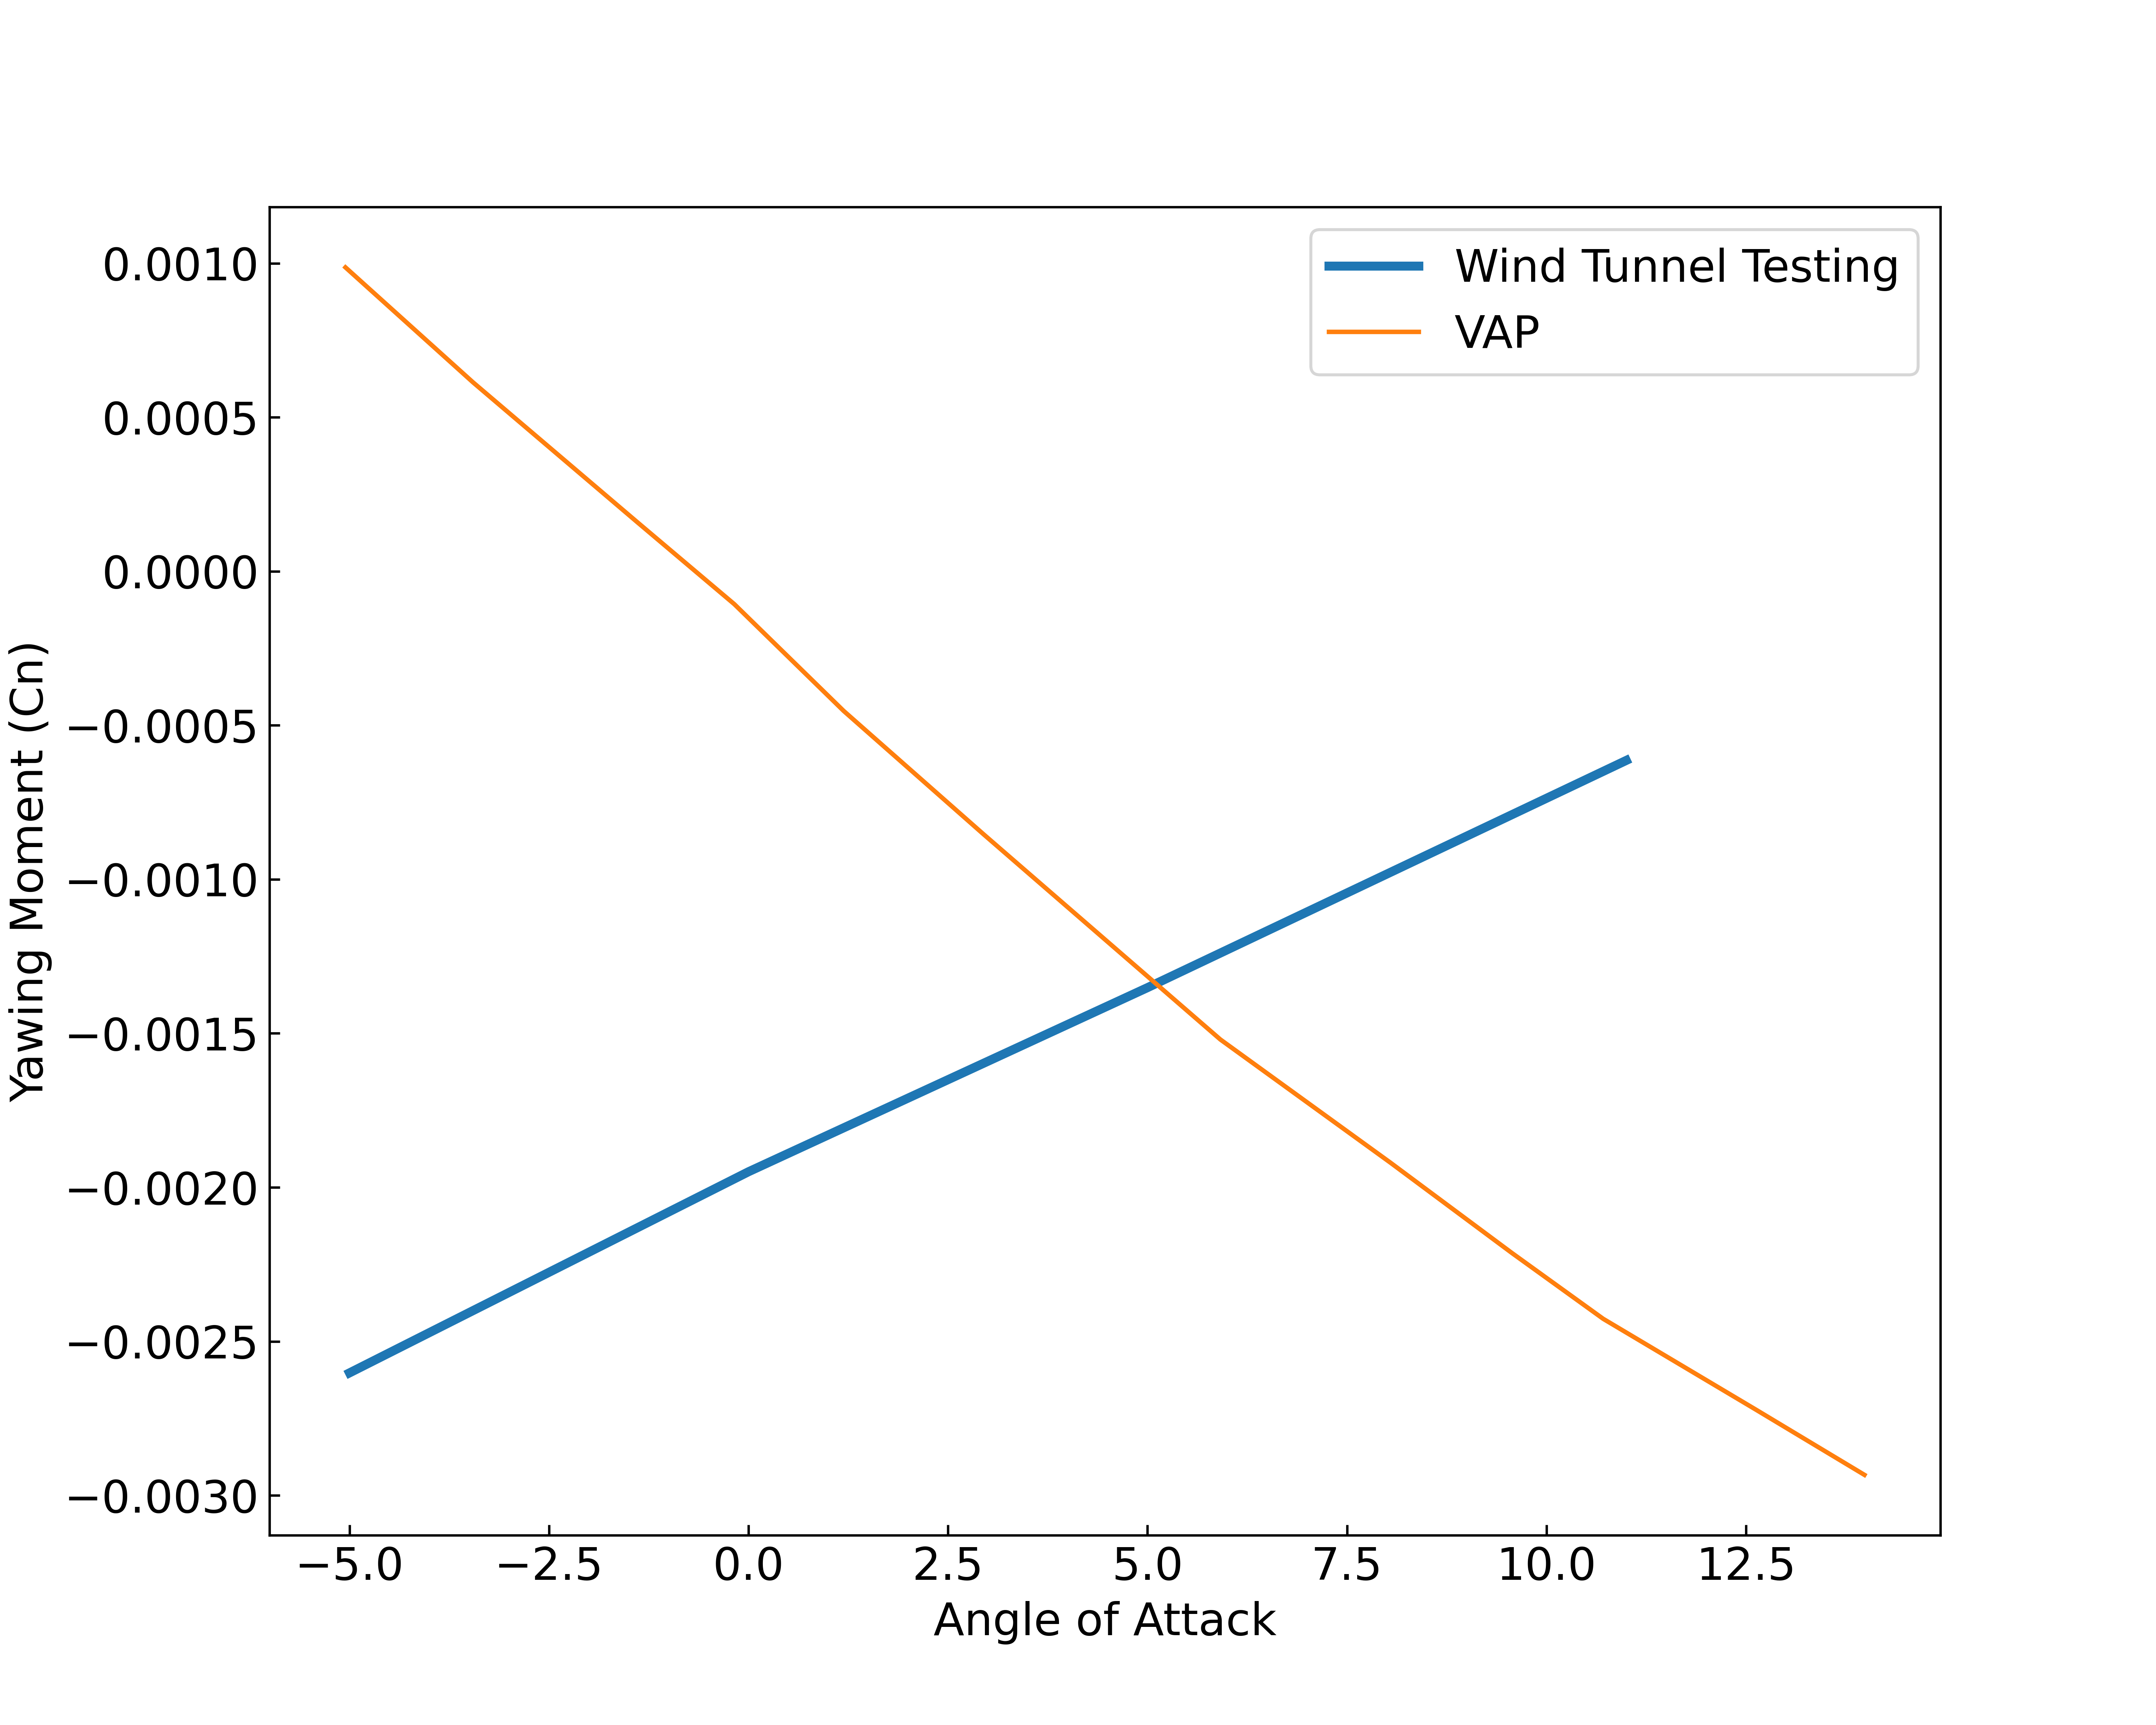
\includegraphics[width=\textwidth]{05_Results/VAP/noProp/Cn/20ms_6000RPM_Cn.png}
        \caption{Yawing Moment Coefficient at 20m/s airspeed and 6000RPM motor speed}
        \label{fig:VAP_noProp_Cm_20ms_6000}
    \end{subfigure}
    \begin{subfigure}[b]{0.467\textwidth}
        \centering
        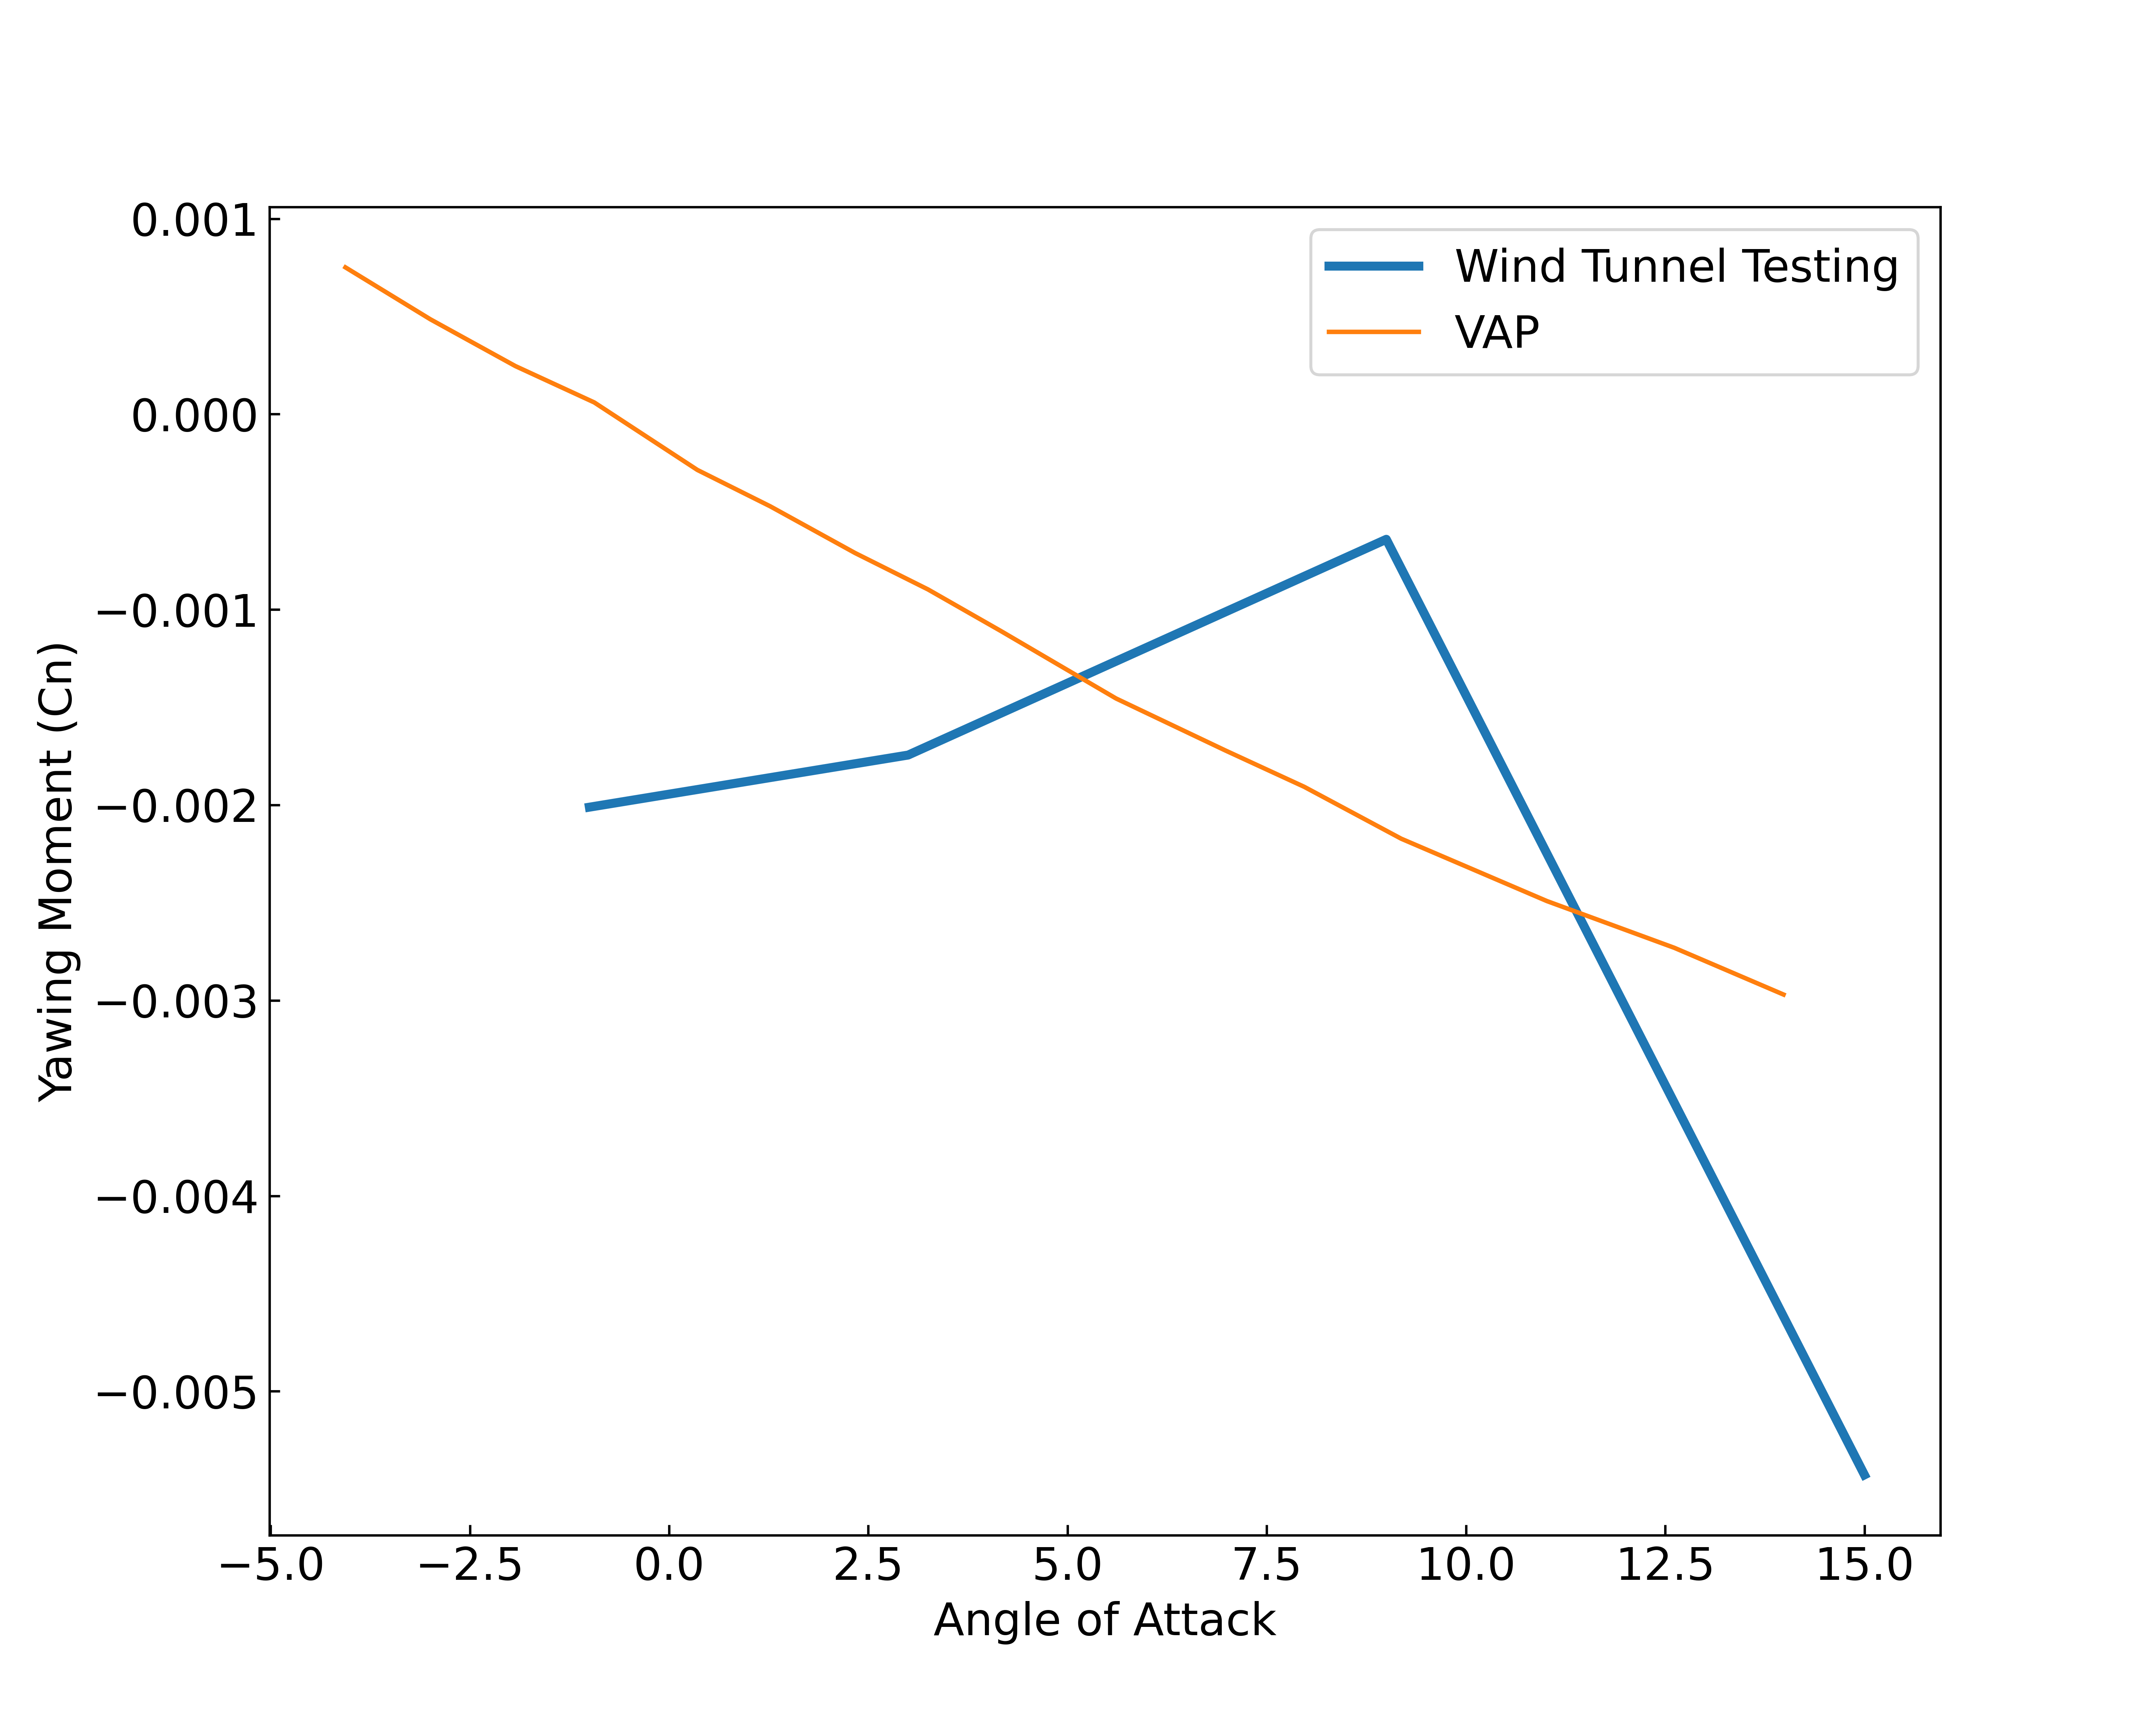
\includegraphics[width=\textwidth]{05_Results/VAP/noProp/Cn/20ms_11000RPM_Cn.png}
        \caption{Yawing Moment Coefficient at 20m/s airspeed and 11000RPM motor speed}
        \label{fig:VAP_noProp_Cm_20ms_11000}
    \end{subfigure}
\end{figure}



\subsubsection{Tractor Configuration}



\begin{figure}[H]
    \centering
    \begin{subfigure}[b]{0.467\textwidth}
        \centering
        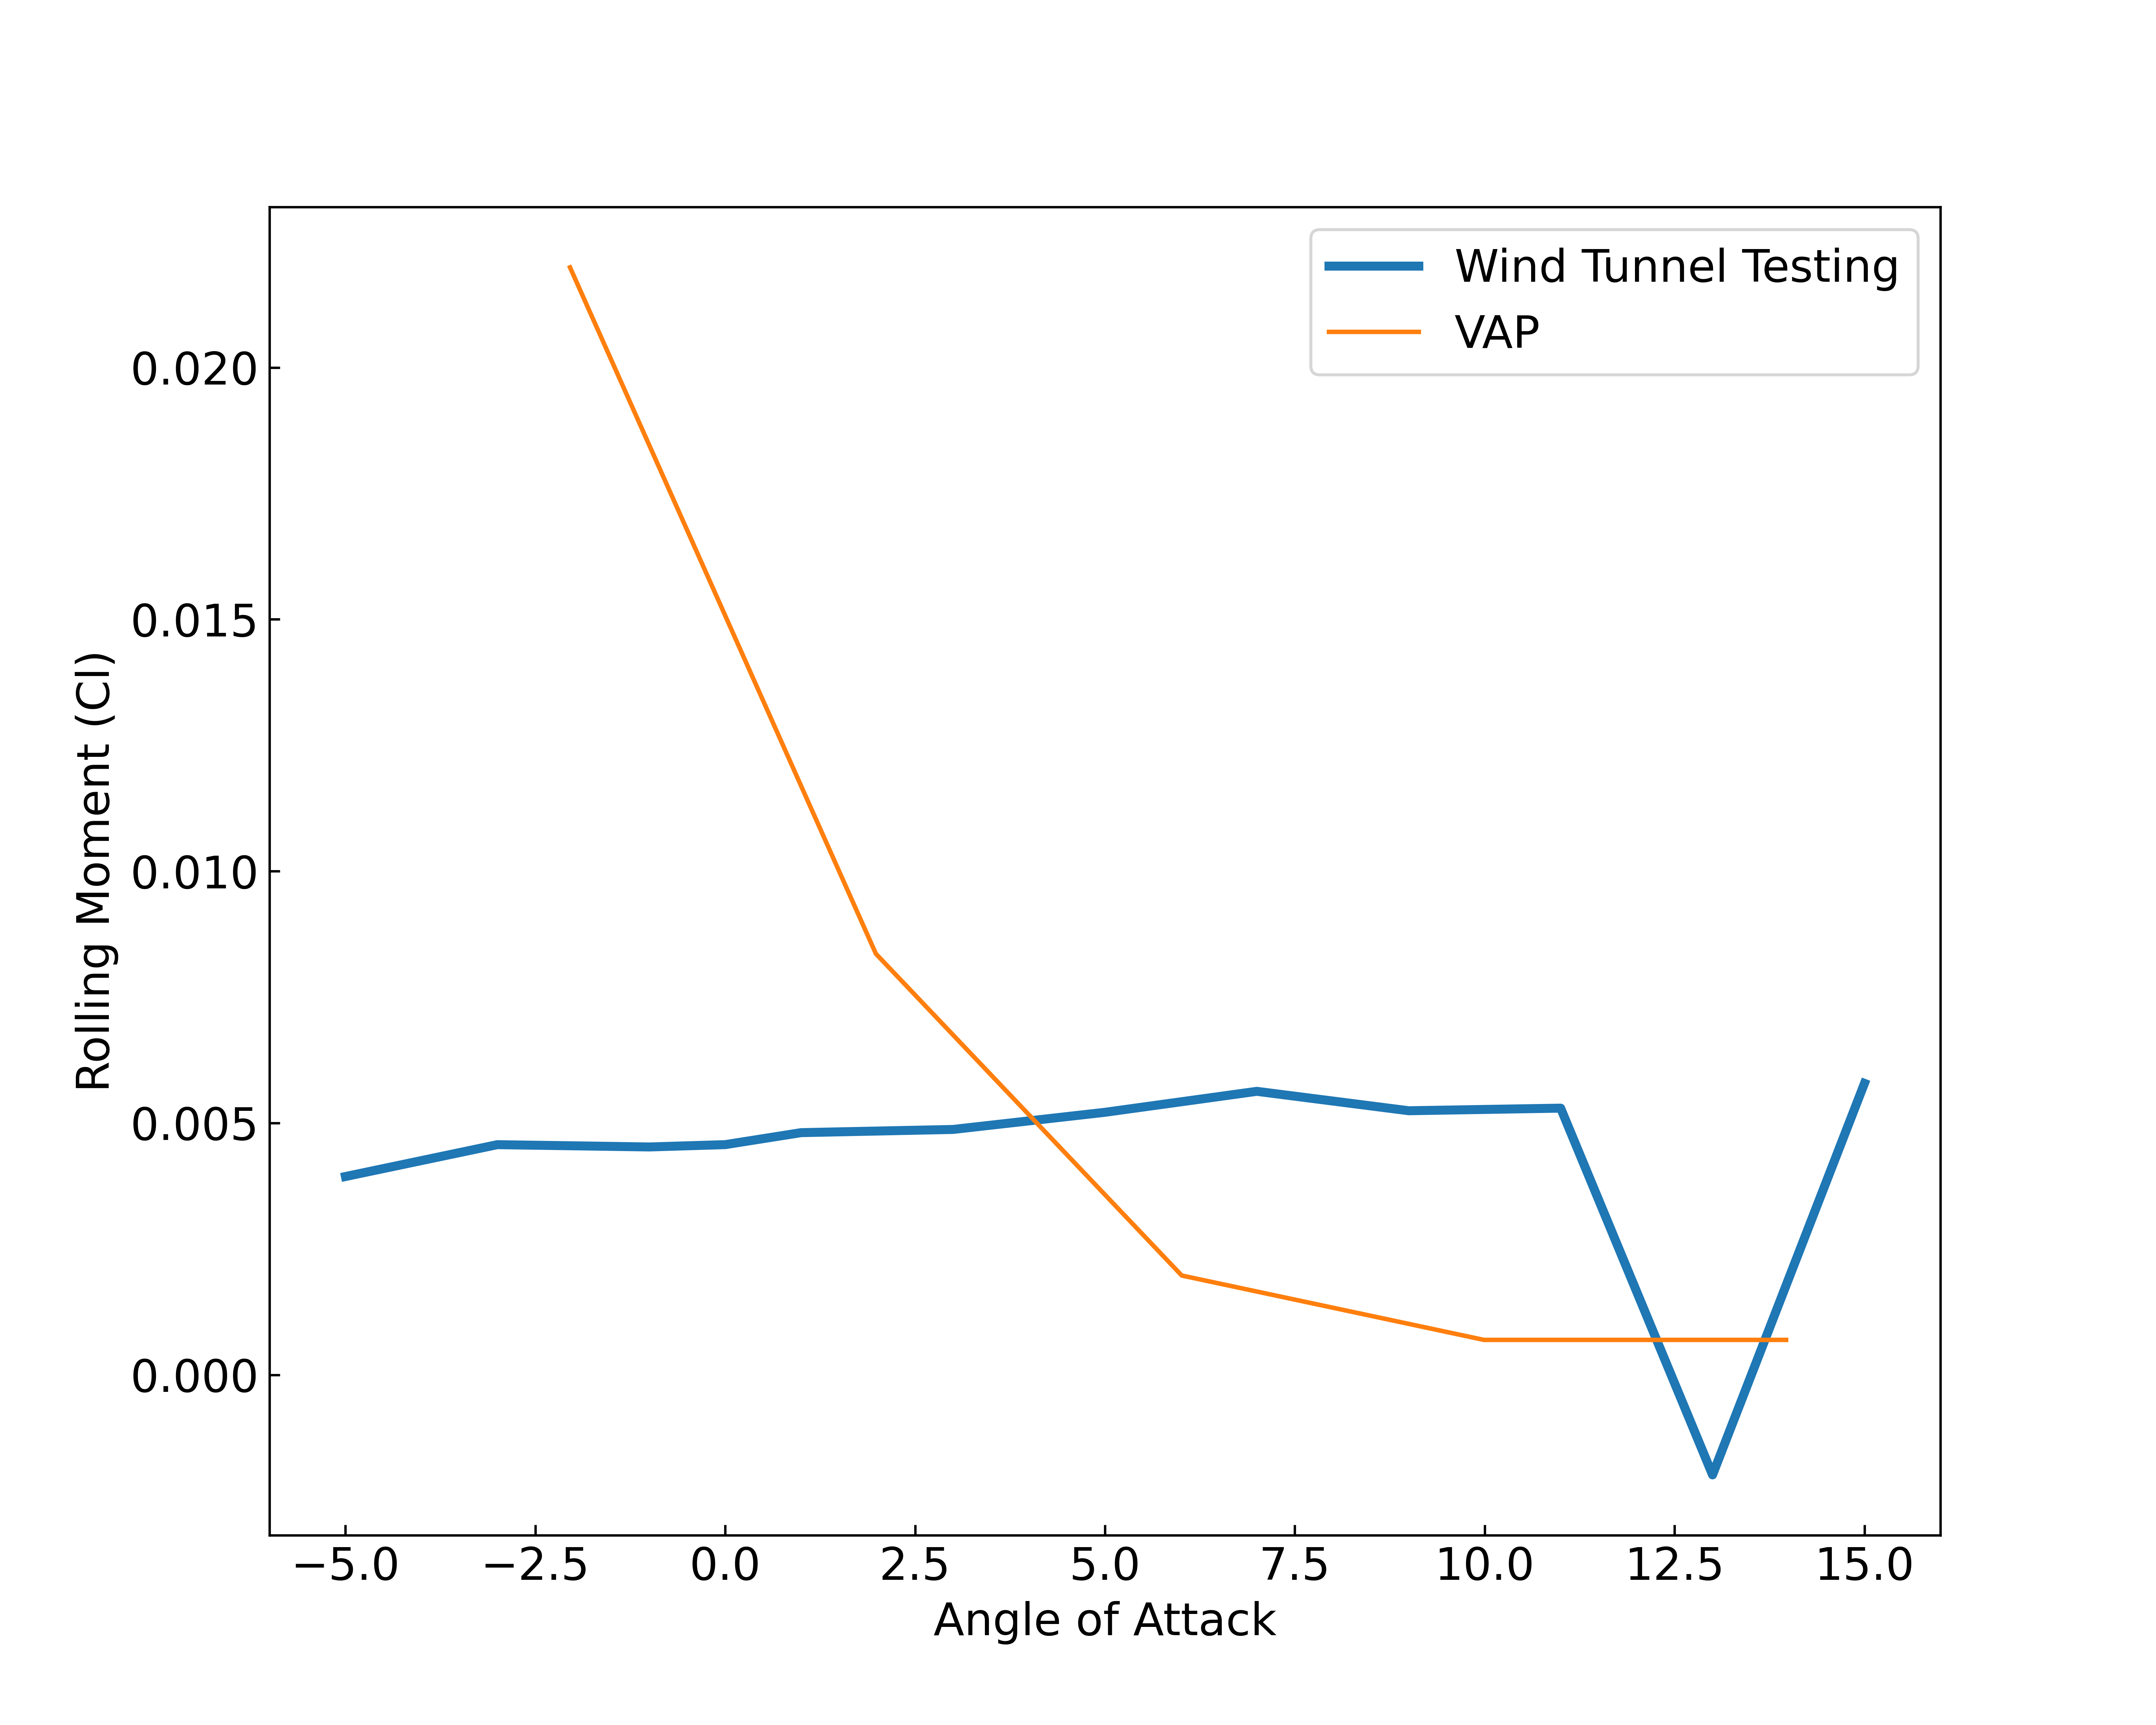
\includegraphics[width=\textwidth]{05_Results/VAP/tractor/Cl/10ms_6000RPM_Cl.png}
        \caption{Rolling Moment Coefficient at 10m/s airspeed and 6000RPM motor speed}
        \label{fig:VAP_Cl_10ms_6000}
    \end{subfigure}
    \begin{subfigure}[b]{0.467\textwidth}
        \centering
        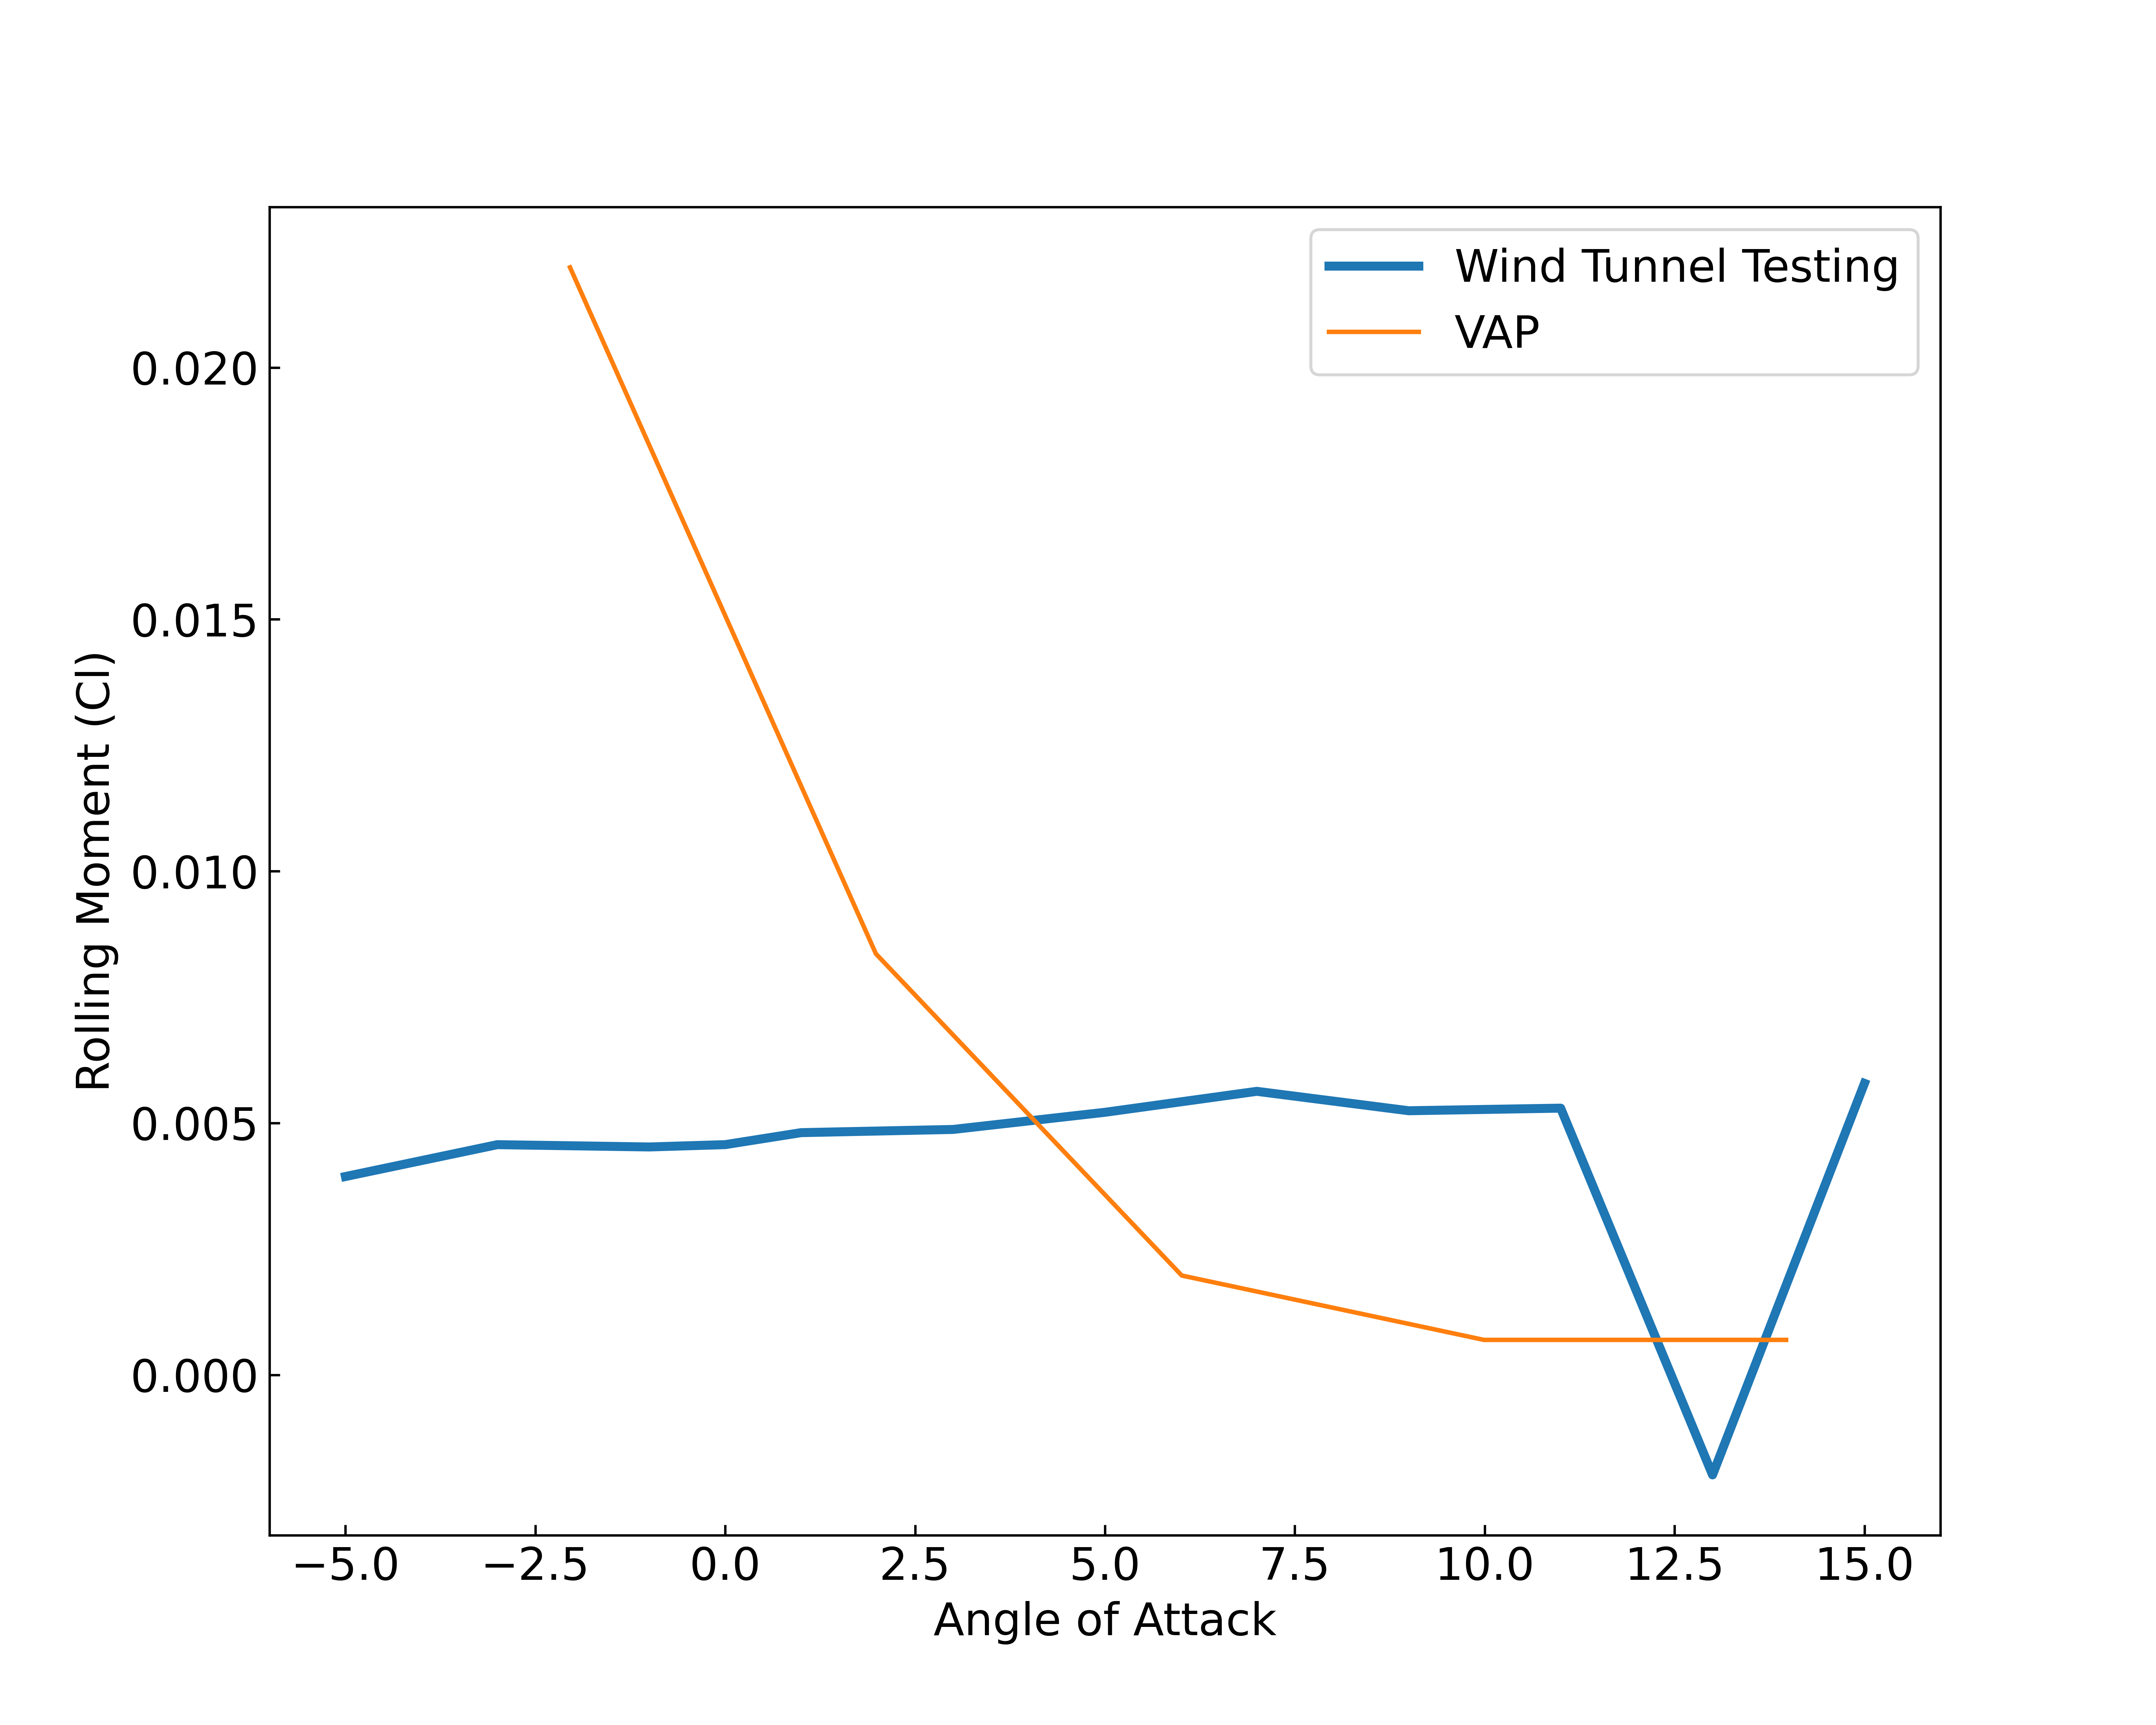
\includegraphics[width=\textwidth]{05_Results/VAP/tractor/Cl/10ms_6000RPM_Cl.png}
        \caption{Rolling Moment Coefficient at 10m/s airspeed and 11000RPM motor speed}
        \label{fig:Missing2}
    \end{subfigure}
    \begin{subfigure}[b]{0.467\textwidth}
        \centering
        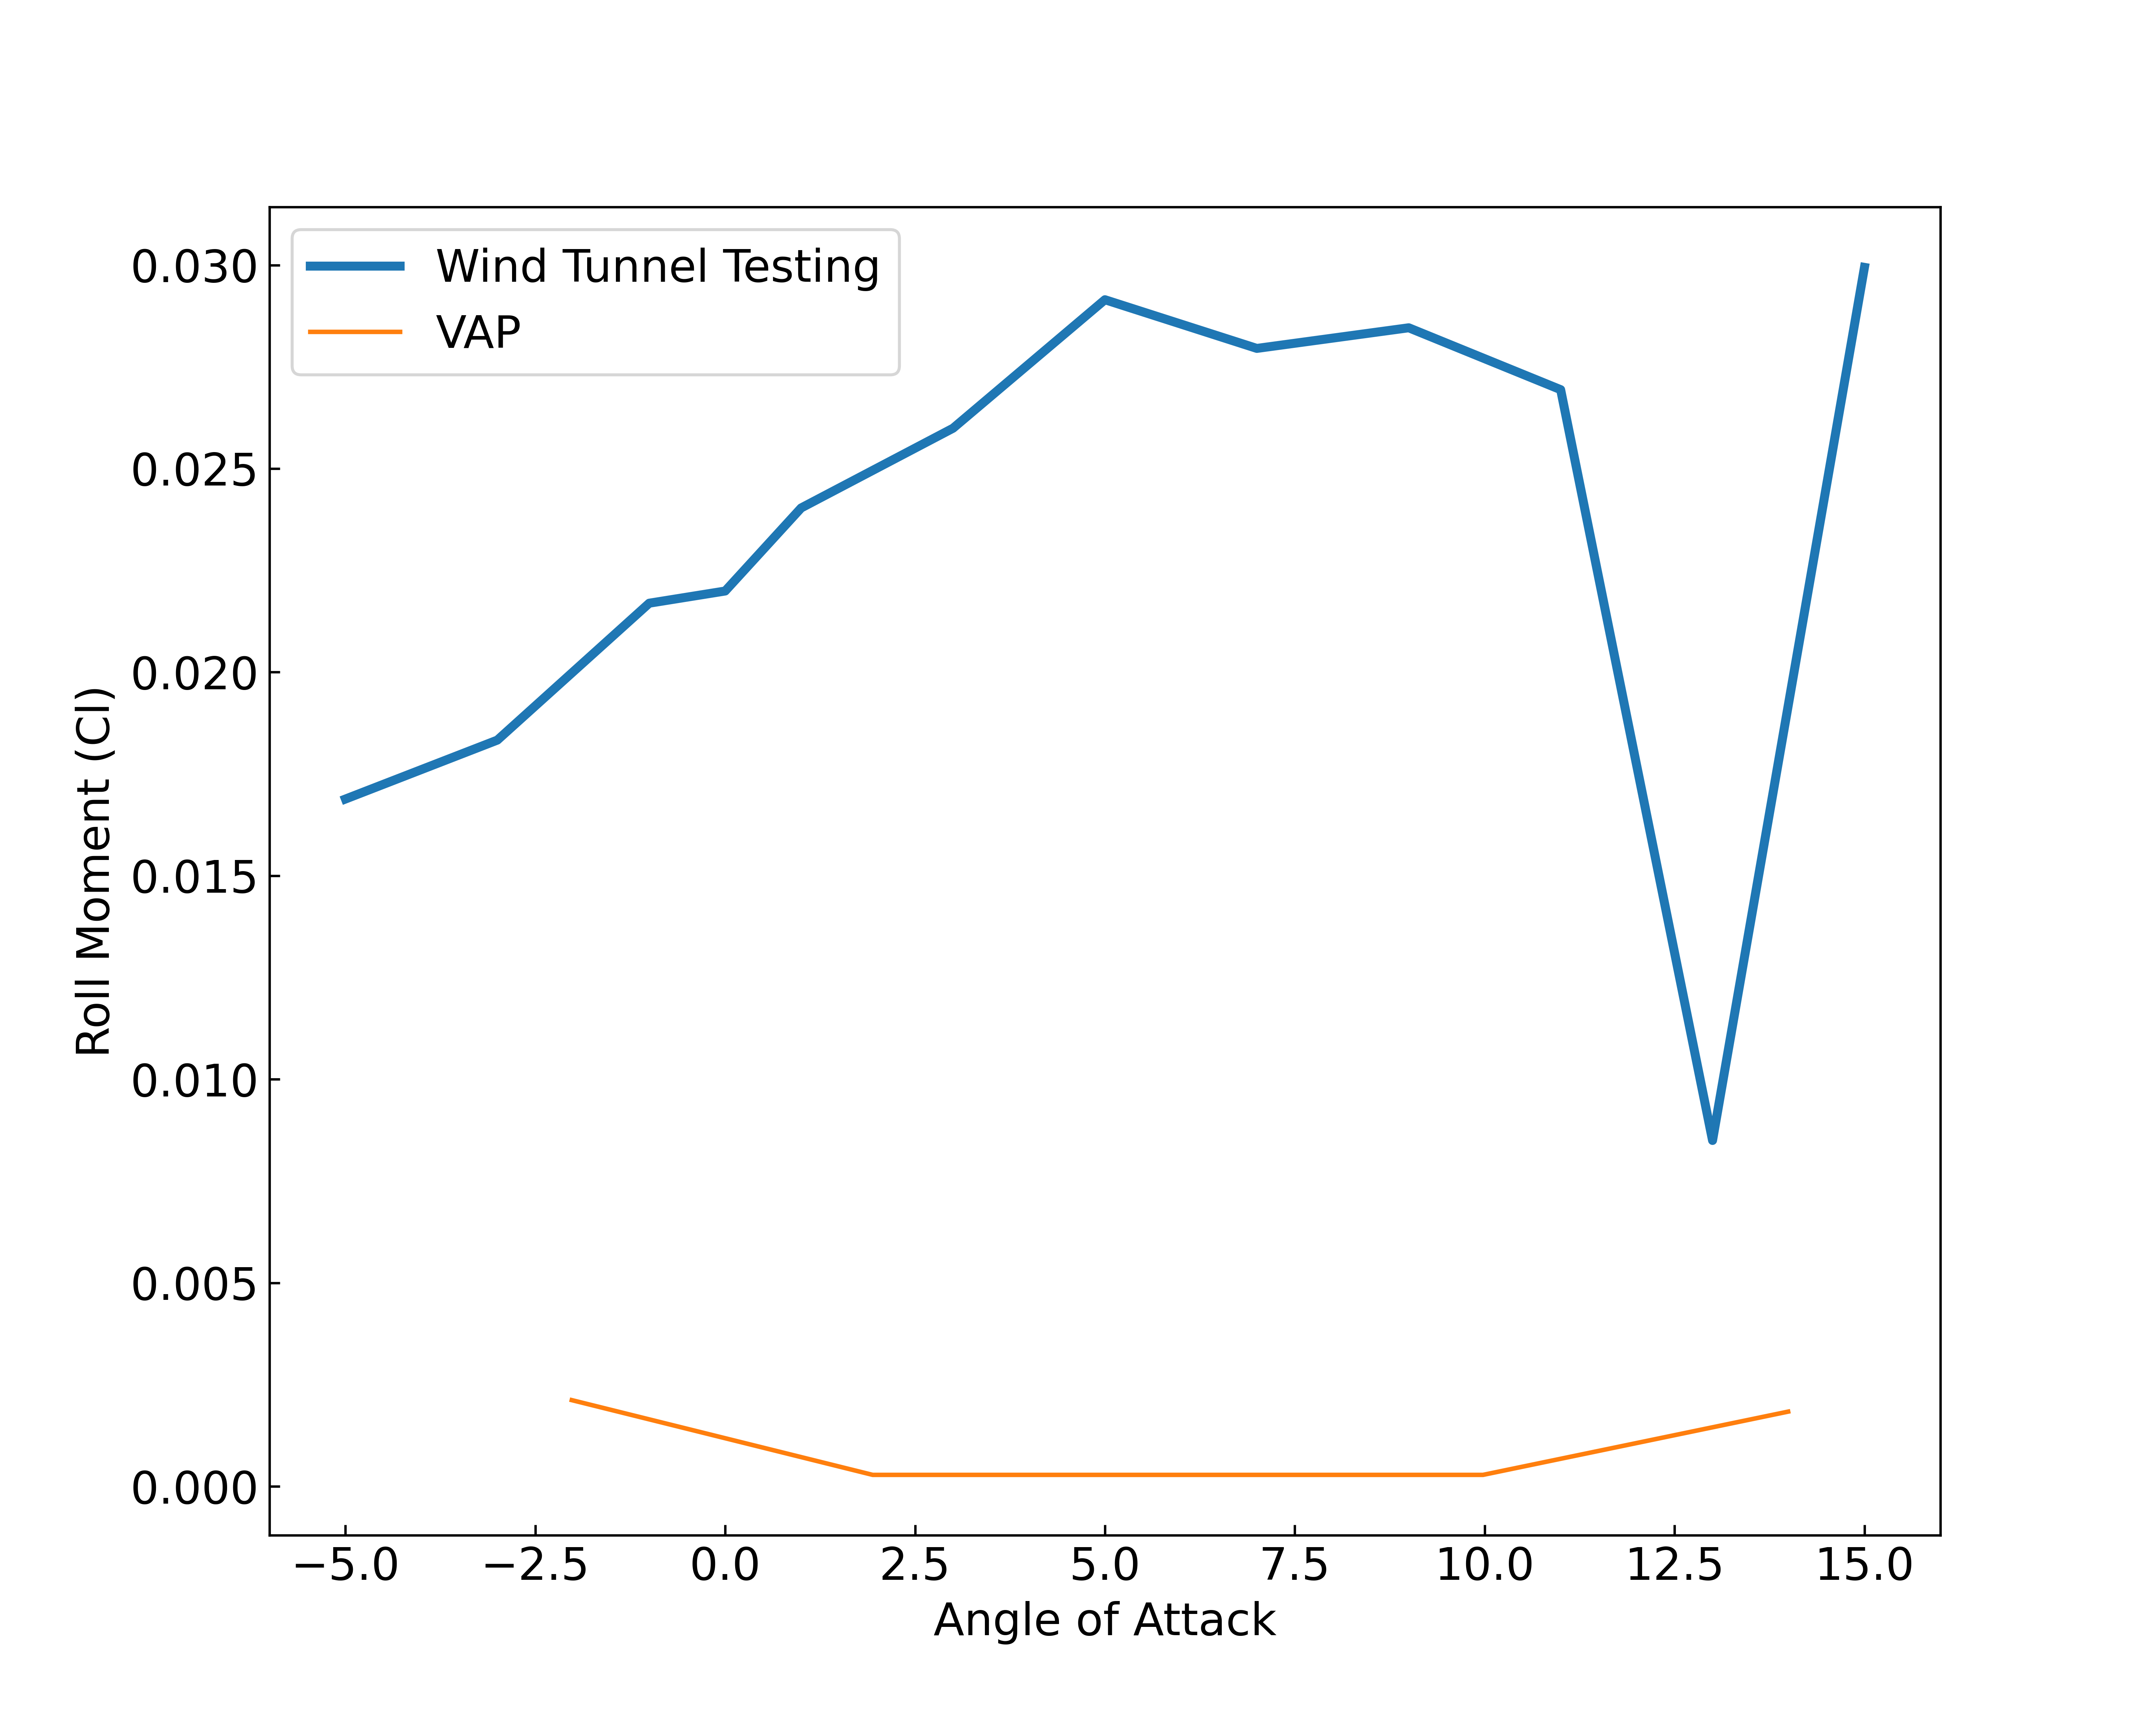
\includegraphics[width=\textwidth]{05_Results/VAP/tractor/Cl/20ms_6000RPM_Cl.png}
        \caption{Rolling Moment Coefficient at 20m/s airspeed and 6000RPM motor speed}
        \label{fig:VAP_Cl_20ms_6000}
    \end{subfigure}
    \begin{subfigure}[b]{0.467\textwidth}
        \centering
        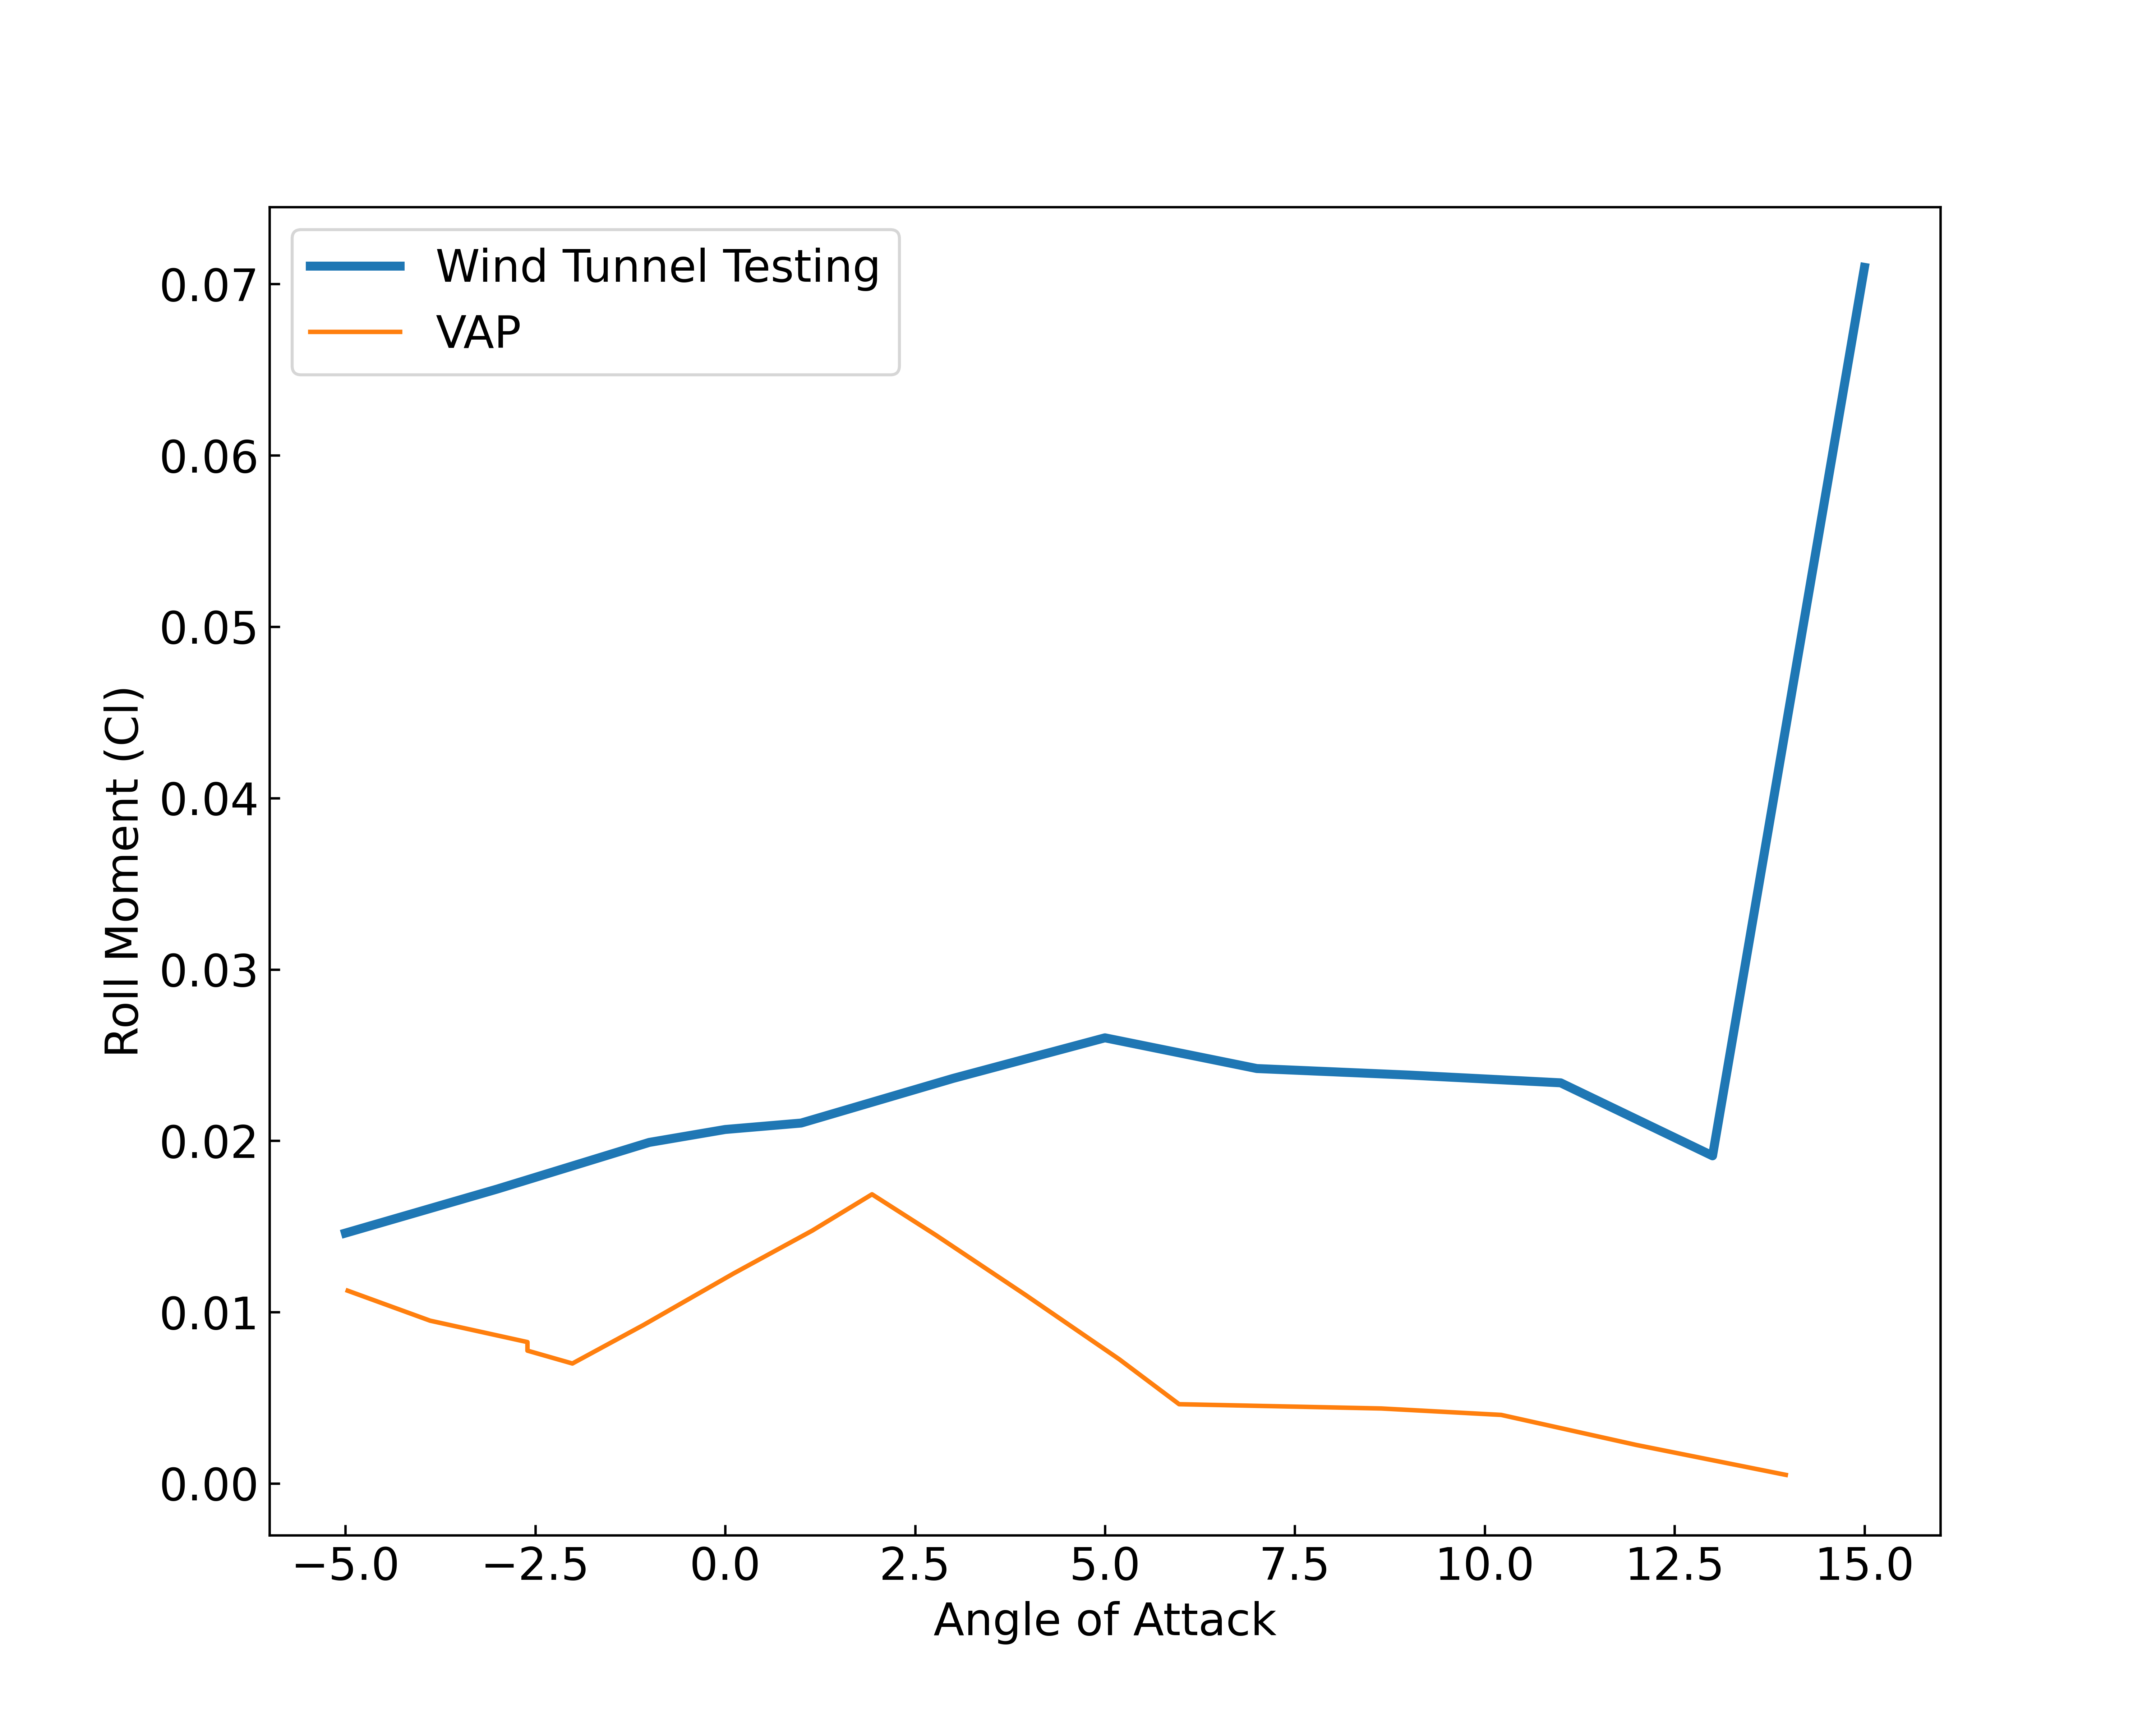
\includegraphics[width=\textwidth]{05_Results/VAP/tractor/Cl/20ms_11000RPM_Cl.png}
        \caption{Rolling Moment Coefficient at 20m/s airspeed and 11000RPM motor speed}
        \label{fig:VAP_Cl_20ms_11000}
    \end{subfigure}
\end{figure}


\begin{figure}[H]
    \centering
    \begin{subfigure}[b]{0.467\textwidth}
        \centering
        \includegraphics[width=\textwidth]{05_Results/VAP/tractor/Cm/10ms_6000RPM_Cm.png}
        \caption{Pitching Moment Coefficient at 10m/s airspeed and 6000RPM motor speed}
        \label{fig:VAP_Cm_10ms_6000}
    \end{subfigure}
    \begin{subfigure}[b]{0.467\textwidth}
        \centering
        \includegraphics[width=\textwidth]{05_Results/VAP/tractor/Cm/10ms_11000RPM_Cm.png}
        \caption{Pitching Moment Coefficient at 10m/s airspeed and 11000RPM motor speed}
        \label{fig:VAP_Cm_10ms_11000}
    \end{subfigure}
    \begin{subfigure}[b]{0.467\textwidth}
        \centering
        \includegraphics[width=\textwidth]{05_Results/VAP/tractor/Cm/20ms_6000RPM_Cm.png}
        \caption{Pitching Moment Coefficient at 20m/s airspeed and 6000RPM motor speed}
        \label{fig:VAP_Cm_20ms_6000}
    \end{subfigure}
    \begin{subfigure}[b]{0.467\textwidth}
        \centering
        \includegraphics[width=\textwidth]{05_Results/VAP/tractor/Cm/20ms_11000RPM_Cm.png}
        \caption{Pitching Moment Coefficient at 20m/s airspeed and 11000RPM motor speed}
        \label{fig:VAP_Cm_20ms_11000}
    \end{subfigure}
\end{figure}



\begin{figure}[H]
    \centering
    \begin{subfigure}[b]{0.467\textwidth}
        \centering
        \includegraphics[width=\textwidth]{05_Results/VAP/tractor/Cn/10ms_11000RPM_Cn.png}
        \caption{Yawing Moment Coefficient at 10m/s airspeed and 6000RPM motor speed}
        \label{fig:missing}
    \end{subfigure}
    \begin{subfigure}[b]{0.467\textwidth}
        \centering
        \includegraphics[width=\textwidth]{05_Results/VAP/tractor/Cn/10ms_11000RPM_Cn.png}
        \caption{Yawing Moment Coefficient at 10m/s airspeed and 11000RPM motor speed}
        \label{fig:VAP_tractor_10ms_11000}
    \end{subfigure}
    \begin{subfigure}[b]{0.467\textwidth}
        \centering
        \includegraphics[width=\textwidth]{05_Results/VAP/tractor/Cn/20ms_6000RPM_Cn.png}
        \caption{Yawing Moment Coefficient at 20m/s airspeed and 6000RPM motor speed}
        \label{fig:VAP_Cn_20ms_6000}
    \end{subfigure}
    \begin{subfigure}[b]{0.467\textwidth}
        \centering
        \includegraphics[width=\textwidth]{05_Results/VAP/tractor/Cn/20ms_11000RPM_Cn.png}
        \caption{Yawing Moment Coefficient at 20m/s airspeed and 11000RPM motor speed}
        \label{fig:VAP_Cn_20ms_11000}
    \end{subfigure}
\end{figure}


\subsubsection{Pusher Configuration}
\begin{figure}[H]
    \centering
    \begin{subfigure}[b]{0.467\textwidth}
      \centering
        \includegraphics[width=\textwidth]{05_Results/Figs/VAP/fullyDevelopedWake.png}
        \caption{}
        \label{fig:TractorCofigurationWake}
         \end{subfigure}
          \begin{subfigure}[b]{0.467\textwidth}
      \centering
        \includegraphics[width=\textwidth]{05_Results/Figs/VAP/fullyDevelopedWake2.png}
        \caption{}
        \label{fig:TractorCofigurationWake2}
         \end{subfigure}
\end{figure}


\begin{figure}[H]
    \centering
    \begin{subfigure}[b]{0.467\textwidth}
        \centering
        \includegraphics[width=\textwidth]{05_Results/VAP/pusher/Cl/10ms_6000RPM_Cl.png}
        \caption{Rolling Moment Coefficient at 10m/s airspeed and 6000RPM motor speed}
        \label{fig:VAP_pusher_Cl_10ms_6000}
    \end{subfigure}
    \begin{subfigure}[b]{0.467\textwidth}
        \centering
        \includegraphics[width=\textwidth]{05_Results/VAP/pusher/Cl/10ms_11000RPM_Cl.png}
        \caption{Rolling Moment Coefficient at 10m/s airspeed and 11000RPM motor speed}
        \label{fig:VAP_pusher_Cl_10ms_11000}
    \end{subfigure}
    \begin{subfigure}[b]{0.467\textwidth}
        \centering
        \includegraphics[width=\textwidth]{05_Results/VAP/pusher/Cl/20ms_6000RPM_Cl.png}
        \caption{Rolling Moment Coefficient at 20m/s airspeed and 6000RPM motor speed}
        \label{fig:VAP_psuher_Cl_20ms_6000}
    \end{subfigure}
    \begin{subfigure}[b]{0.467\textwidth}
        \centering
        \includegraphics[width=\textwidth]{05_Results/VAP/pusher/Cl/20ms_11000RPM_Cl.png}
        \caption{Rolling Moment Coefficient at 20m/s airspeed and 11000RPM motor speed}
        \label{fig:VAP_pusher_Cl_20ms_11000}
    \end{subfigure}
\end{figure}


\begin{figure}[H]
    \centering
    \begin{subfigure}[b]{0.467\textwidth}
        \centering
        \includegraphics[width=\textwidth]{05_Results/VAP/pusher/Cm/10ms_6000RPM_Cm.png}
        \caption{Pitching Moment Coefficient at 10m/s airspeed and 6000RPM motor speed}
        \label{fig:VAP_pusher_Cm_10ms_6000}
    \end{subfigure}
    \begin{subfigure}[b]{0.467\textwidth}
        \centering
        \includegraphics[width=\textwidth]{05_Results/VAP/pusher/Cm/10ms_11000RPM_Cm.png}
        \caption{Pitching Moment Coefficient at 10m/s airspeed and 11000RPM motor speed}
        \label{fig:VAP_pusher_Cm_10ms_11000}
    \end{subfigure}
    \begin{subfigure}[b]{0.467\textwidth}
        \centering
        \includegraphics[width=\textwidth]{05_Results/VAP/pusher/Cm/20ms_6000RPM_Cm.png}
        \caption{Pitching Moment Coefficient at 20m/s airspeed and 6000RPM motor speed}
        \label{fig:VAP_pusher_Cm_20ms_6000}
    \end{subfigure}
    \begin{subfigure}[b]{0.467\textwidth}
        \centering
        \includegraphics[width=\textwidth]{05_Results/VAP/pusher/Cm/20ms_11000RPM_Cm.png}
        \caption{Pitching Moment Coefficient at 20m/s airspeed and 11000RPM motor speed}
        \label{fig:VAP_pusher_Cm_20ms_11000}
    \end{subfigure}
\end{figure}



\begin{figure}[H]
    \centering
    \begin{subfigure}[b]{0.467\textwidth}
        \centering
        \includegraphics[width=\textwidth]{05_Results/VAP/pusher/Cn/10ms_6000RPM_Cn.png}
        \caption{Yawing Moment Coefficient at 10m/s airspeed and 6000RPM motor speed}
        \label{fig:VAP_pusher_Cn_10ms_6000}
    \end{subfigure}
    \begin{subfigure}[b]{0.467\textwidth}
        \centering
        \includegraphics[width=\textwidth]{05_Results/VAP/pusher/Cn/10ms_11000RPM_Cn.png}
        \caption{Yawing Moment Coefficient at 10m/s airspeed and 11000RPM motor speed}
        \label{fig:VAP_pusherr_Cn_10ms_11000}
    \end{subfigure}
    \begin{subfigure}[b]{0.467\textwidth}
        \centering
        \includegraphics[width=\textwidth]{05_Results/VAP/pusher/Cn/20ms_6000RPM_Cn.png}
        \caption{Yawing Moment Coefficient at 20m/s airspeed and 6000RPM motor speed}
        \label{fig:VAP_pusher_Cn_20ms_6000}
    \end{subfigure}
    \begin{subfigure}[b]{0.467\textwidth}
        \centering
        \includegraphics[width=\textwidth]{05_Results/VAP/pusher/Cn/20ms_11000RPM_Cn.png}
        \caption{Yawing Moment Coefficient at 20m/s airspeed and 11000RPM motor speed}
        \label{fig:VAP_pusher_Cn_20ms_11000}
    \end{subfigure}
\end{figure}


\section{Discussion}